\documentclass[sigconf, review]{acmart}


\usepackage{enumitem}
\setlist[description]{leftmargin=\parindent,labelindent=\parindent}

\usepackage{xcolor}
%\usepackage{amsmath}
\usepackage{listingsutf8}
\usepackage{hyperref}
\usepackage{graphicx}
\usepackage{tabularx}
\usepackage{xspace}
\usepackage{textcomp}
\usepackage{wasysym,stmaryrd}
\usepackage{mathpartir}
\usepackage{url}
%\usepackage{upgreek}
\usepackage{xparse}
\usepackage{booktabs}
\usepackage[utf8]{inputenc}
\usepackage[T1]{fontenc}
%\usepackage{stix}
\usepackage{placeins} % for \FloatBarrier

\usepackage{algorithm}
\usepackage{algpseudocode}

\usepackage[export]{adjustbox}

%\usepackage{algorithm}
%\usepackage{algpseudocode}

\usepackage{enumitem}

\usepackage{wrapfig}
\usepackage{fancyvrb}

\usepackage{caption}

\usepackage{makecell}

\usepackage{varwidth}
\DeclareCaptionFormat{nastyCaption}{%
  % #1: label (e.g. "Table 1")
  % #2: separator (e.g. ": ")
  % #3: caption text
  \begin{varwidth}{\linewidth}%
    \centering
    #1#2#3%
  \end{varwidth}%
}

\setlist[description]{leftmargin=\parindent,labelindent=\parindent}

\usepackage{subcaption}

\makeatletter
\newif\ifFV@bgcolor
\newbox\FV@bgbox
\define@key{FV}{bgcolor}{\FV@bgcolortrue\def\FV@bgcolor{#1}}

\def\FV@BeginVBox{%
  \leavevmode\ifFV@bgcolor\setbox\FV@bgbox=\fi
  \hbox\ifx\FV@boxwidth\relax\else to\FV@boxwidth\fi\bgroup
  \ifcase\FV@baseline\vbox\or\vtop\or$\vcenter\fi\bgroup}
\def\FV@EndVBox{\egroup\ifmmode$\fi\hfil\egroup
  \ifFV@bgcolor\colorbox{\FV@bgcolor}{\box\FV@bgbox}\fi}
\makeatother

\newcommand{\shat}{\^{s}}

%JavaScript 
\definecolor{SkyBlue}{rgb}{0.20,0.39,0.64}
\definecolor{Plum}{rgb}{0.46,0.31,0.48}
\definecolor{Chocolate}{rgb}{0.75,0.49,0.07}
\definecolor{Aluminium5}{rgb}{0.33,0.34,0.32}
\definecolor{DarkGreen}{rgb}{0.2,0.5,0.2}
\definecolor{ltblue}{rgb}{0,0.4,0.4}
\definecolor{dkblue}{rgb}{0,0.2,0.7}
\definecolor{dkgreen}{rgb}{0,0.4,0}
\definecolor{dkviolet}{rgb}{0.3,0,0.5}
\definecolor{dkred}{rgb}{0.6,0,0}
\definecolor{talkred}{rgb}{0.69,.20,0.22}
\definecolor{talkblue}{rgb}{0.04,0.40,0.80}
\definecolor{talkgreen}{rgb}{0.34,.81,0.10}
\definecolor{oldtalkblue}{rgb}{0.22,.20,0.69}
\definecolor{greenish}{rgb}{.0,.65,.0}
\definecolor{mygray}{gray}{0.9}

\lstset{
	showstringspaces=false
}

\lstdefinelanguage{JavaScript}{
  morekeywords=[1]{typeof, new, true, false, catch,
    function, return, null, catch, switch, var,
    if, in, while, do, else, case, break, continue},
  morekeywords=[2]{class, export, boolean, throw, implements, import, this},
  numbers=left,
  numbersep=4pt,
  numberstyle=\tiny\color{dkblue},
  columns=fullflexible,
  sensitive=false,
  comment=[l]{//},
  captionpos=b,   
  morecomment=[s]{/*}{*/},
  morestring=[b]',
  morestring=[b]",
  basicstyle=\scriptsize\texttt,
  identifierstyle=\ttfamily\color{Aluminium5},
  keywordstyle=[1]\ttfamily\color{Plum},
  keywordstyle=[2]\ttfamily\color{SkyBlue},
  stringstyle=\ttfamily\color{DarkGreen},
  commentstyle=\ttfamily, 
%  commandchars=\$\{\}
}[keywords,comments,strings]

\lstdefinelanguage{Scheme}{
  morekeywords=[1]{define, define-syntax, define-macro, lambda, define-stream, stream-lambda},
  morekeywords=[2]{begin, call-with-current-continuation, call/cc,
    call-with-input-file, call-with-output-file, case, cond,
    do, else, for-each, if,
    let*, let, let-syntax, letrec, letrec-syntax,
    let-values, let*-values,
    and, or, not, delay, force,
    quasiquote, quote, unquote, unquote-splicing,
    map, fold, syntax, syntax-rules, eval, environment, query },
  morekeywords=[3]{import, export},
  alsodigit=!\$\%&*+-./:<=>?@^_~,
  sensitive=true,
  morecomment=[l]{;},
  morecomment=[s]{\#|}{|\#},
  morestring=[b]",
  basicstyle=\scriptsize\ttfamily,
  keywordstyle=\bf\ttfamily\color[rgb]{0,.3,.7},
  commentstyle=\color[rgb]{0.133,0.545,0.133},
  stringstyle={\color[rgb]{0.75,0.49,0.07}},
  upquote=true,
  breaklines=true,
  breakatwhitespace=true,
  literate=*{`}{{`}}{1}
}

\def\schemeinline{\lstinline[language=Scheme, basicstyle=\small\ttfamily]}

\lstnewenvironment{lstjs}{\lstset{language=JavaScript,basicstyle=\fontsize{8}{8}\ttfamily,escapeinside={~}{~}}}{}
\def\jsinline{\lstinline[language=JavaScript, basicstyle=\small]}


% The Acronyms of the project and some other stuff
\newcommand{\jsil}{JSIL\xspace}
\newcommand{\jsverify}{JSVerify\xspace}
\newcommand{\JSComp}{JS-2-JSIL\xspace}
\newcommand{\jsilverify}{JSILVerify\xspace}


% Tikz 
\usepackage{tikz}
\usetikzlibrary{calc,positioning,arrows,shapes,decorations.pathmorphing}
\usetikzlibrary{arrows,positioning} 
\tikzset{
    %Define standard arrow tip
    >=stealth',
    % Define arrow style
    pil/.style={
           ->,
           shorten <=2pt,
           shorten >=2pt,}
}

\newcommand{\runpic}{\includegraphics[width=0.06\picwidth]{running.pdf}}
\newcommand{\tickpic}{\resizebox{0.06\picwidth}{!}{\(\color{greenish} \checkmark \)}}
\tikzset{
  box/.style = {rectangle, draw=black,align=center,font=\scriptsize},
  sbox/.style = {rectangle,draw=black,align=left,font=\scriptsize,text width=1.7cm},
  p/.style = {-latex},
  dp/.style = {latex-latex},
  sz/.style n args={2}{minimum width=#2, minimum height=#1},
  m/.style = {midway,inner sep=0pt,fill=white},
  ll/.style = {font=\scriptsize,anchor=south west}
}



% Polishing...
\newcommand{\polish}[1]{{\color{red}#1}}


\usepackage{cosette_macros}


% macros_js as for Jose Santos
%\usepackage{macros_js}
%\usepackage{gdshojs}

\newcommand{\cosette}{Cosette\xspace}
\newcommand{\rosette}{Rosette\xspace}

\newcommand{\myparagraph}[1]{\smallskip\noindent {\bf #1.}\hspace{1pt}}
\newcommand{\myparagraphq}[1]{\smallskip\noindent {\bf #1?}\hspace{1pt}}

% COMMENTS

\newcommand{\pginline}[1]{ {\color{purple} *** PG : #1 ***} }
\newcommand{\pgmaxinline}[1]{ {\color{purple} *** PG : #1 ***} }
\newcommand{\pmaxinline}[1]{ {\color{blue} *** PM : #1 ***} }
\newcommand{\pinline}[1]{ {\color{blue} *** PM : #1 ***} }
\newcommand{\jfsinline}[1]{ {\color{green} *** JFS : #1 ***} }
\newcommand{\jdinline}[1]{ {\color{green} *** JD : #1 ***} }

\newif\ifComments
\Commentstrue

\newcommand{\pg}[1]{%
\ifComments
\begin{center}
\fbox{\begin{minipage}{0.4\textwidth} \color{red}
{\rm PG: \small #1}
\end{minipage}}
\end{center}
\fi}

\newcommand{\pmax}[1]{%
\ifComments
\begin{center}
\fbox{\begin{minipage}{0.4\textwidth} \color{blue}
{\rm PM: \small #1}
\end{minipage}}
\end{center}
\fi}

\newcommand{\jfs}[1]{%
\ifComments
\begin{center}
\fbox{\begin{minipage}{0.4\textwidth} \color{SkyBlue}
{\rm JFS: \small #1}
\end{minipage}}
\end{center}
\fi}

\newcommand{\jd}[1]{%
\ifComments
\begin{center}
\fbox{\begin{minipage}{0.4\textwidth} \color{purple}
{\rm JD: \small #1}
\end{minipage}}
\end{center}
\fi}

\begin{abstract}
We present \cosette, a framework for trustworthy, compositional symbolic execution of JavaScript programs.
Its aim  is to
  provide \emph{general-purpose} symbolic analysis and {\em assist} 
  developers in the testing of their code: the developer writes symbolic tests for which \cosette provides concrete counter-models.
We create \cosette following a new, general methodology for designing compositional program analyses for dynamic languages.
We prove that the symbolic execution underpinning \cosette is sound
and does not generate false positives. We establish additional trust
by  using the theory to precisely guide the implementation and
by thorough testing.  
We apply Cosette to whole-program symbolic testing of real-world JavaScript libraries and compositional debugging of separation logic specifications of JavaScript programs. 

%Moreover, its compositionality allows us to use \cosette to find bugs in specifications of JS programs that are not detectable by standard symbolic execution techniques.
%\pmaxinline{Now compositionality.}
%
%We evaluate \cosette on challenging examples that showcase JS-specific features, as well as on real-world Node.js libraries, in which we detect several bugs. %These examples involve JavaScript-specific features, such as prototype inheritance, function closures, the for-in statement, and dynamic dispatch. 
%We highlight the range of \cosette by using it to debug %non-trivial 
%separation logic specifications of JS programs. 
%
%It works by compiling JavaScript programs to \jsil using \JSComp, a well-tested, standard-compliant compiler from JavaScript to \jsil, and then symbolically executing the obtained \jsil code using a novel symbolic interpreter for \jsil. We prove that the \jsil symbolic interpreter is \emph{sound} and that it does not generate false positives.
%
%\bigskip
%We present \cosette, a symbolic execution tool for JavaScript (ECMAScript 5, ES5), which precisely follows the language standard. At the core of \cosette is a sound symbolic interpreter for \jsil, an intermediate language well-suited for verification and analysis. This interpreter is written in \underline{Rosette}, %~\cite{Rosette2,Rosette1}, 
%a symbolic virtual machine that enables the design of new solver-aided languages. 
%\cosette works by first compiling JavaScript programs to \jsil using \underline{\JSComp}, %~\cite{javert}, 
%a well-tested, standard-compliant compiler from JavaScript to \jsil, and then symbolically executing the compiled \jsil code in the \jsil symbolic interpreter. 
%We study two complementary uses of \cosette. 
%First, we show how \cosette can be used for symbolic testing of JavaScript programs by finding concrete executions that trigger assertion and test failures. 
%We highlight the range of \cosette by giving examples using strings, regular expressions, and the notorious \jsinline|eval| statement.
%Second, building on \cosette, we develop a tool for debugging separation logic specifications by compiling them to symbolic tests in order to find 
%witnesses for bugs in both specification and code.
%
%\bigskip
%We present \cosette, a framework for bounded symbolic execution of JavaScript (JS) code (ECMAScript 5, ES5). 
%\cosette is the first symbolic execution tool for JS that models the language semantics precisely.  
%It works by first compiling JS programs to \jsil using \JSComp, a well-tested, standard-compliant compiler from 
%JS to \jsil, and then symbolically executing the obtained \jsil code using a novel symbolic interpreter for \jsil. 
%We prove that the \jsil symbolic interpreter is \emph{sound} and that it does not to generate false positives. 
%%every time the tool reports a bug, it provides a concrete model that triggers that bug. 
%
%We demonstrate how \cosette can be used for the symbolic testing of JS programs by 
%finding concrete executions that trigger assertion and test failures. We highlight the range of \cosette 
%by giving examples involving JS-specific features, such as: prototype-based inheritance, 
%the for-in statement, and JS arrays. Finally, we thoroughly evaluate \cosette against a 
%representative fragment of test262 adapted to include symbolic~values.
%
\end{abstract}

\title[\cosette:~Symbolic Execution for JavaScript]{\cosette:~Symbolic Execution for JavaScript}       

\author[J. Fragoso Santos, P. Maksimovi\'c, T. Grohens, J. Dolby, P. Gardner]{Jos\'e Fragoso Santos$^1$, Petar Maksimovi\'c$^1$, Th\'eotime
  Grohens$^2$, Julian Dolby$^3$, Philippa Gardner$^1$}
\affiliation{$^1\ $Imperial College London, $^2\ $ENS Paris, $^3\ $IBM Research}


\begin{document}
%

\maketitle 

%\pgmaxinline{Addresses in title are a bit weird.}

\section{Introduction}
\label{sec:intro}

%\pg{This is what we should answer by the introduction: 
%What's the problem with the current state of the art?
%What is our solution?
%Why is the problem we're solving hard?
%How do we solve the challenges?
%Why do we do better than existing work?
%What are the lessons learnt from the paper?}

%\pmax{Many messages, let's not forget any:
%\begin{itemize}
%\item Methodology for analysis of languages with no frame property
%\item Trustworthiness
%\item Compositionality
%\item Proper description of what we do and not do (soundiness, with or without the term itself) (no eval, for-in with a chosen enumeration)
%\item more...?
%\end{itemize}
%}
%
%%%symbolic execution is...
%

%%JS and symbolic execution, a gap 

%\pgmaxinline{Maybe can summarise the bug patterns, I jsut lifted from related work.}

JavaScript (JS)  is the most widespread dynamic language, used by 95.1\% of websites~\cite{JS948percent}.
Due to its dynamic, complex nature, it is known to be a difficult target for symbolic analysis. 
Recent symbolic execution tools for JavaScript~\cite{saxena:sp:2010,wittern:icse:2018,li:fse:2014} have made significant progress. 
%They focus on specific bug patterns for finding, for example, security vulnerabilities related to the misuse of strings~\cite{saxena:sp:2010}, malformed Web API requests~\cite{wittern:icse:2018}, and bugs arising from the DOM API~\cite{li:fse:2014}. 
They are fully automatic, aim at code in the large, and primarily
focus on scalability and coverage issues.  However, these tools do have some
limitations. They only target specific bug
patterns rather than general-purpose symbolic execution, and depend on
whole-program analysis.

Whole-program analysis is not sufficient for JavaScript applications, 
which are commonly run in highly dynamic execution
environments: for example, client-side programs dynamically load and
execute third-party code as a matter of course. One also needs to be
able to analyse incomplete code in a compositional manner.
Designing compositional analyses for dynamic languages such as JavaScript, 
however, is non-trivial. This is because, unlike static languages
such as C, C++ and Java, dynamic languages do not observe the
\emph{frame property}~\cite{reynolds:lics:2002}, essential for
compositionality. Intuitively, the frame property means that the
output of a program cannot change if the state in which it is run is
extended. In JavaScript, it is possible to introduce bugs by 
extending the state in which a program is run. To our knowledge, 
there has been no previous work on compositional symbolic execution
for JavaScript.

%Unlike static languages such as C, C++ and Java, JavaScript does 
%not observe the \emph{frame property}~\cite{reynolds:lics:2002}. 
%Intuitively, the frame property means that the output of a program 
%cannot change if the state in which is run is extended. 
%In JavaScript, it is possible to introduce bugs by extending the 
%state in which a program is run.

%Also, they do not come with formal correctness guarantees.

%% another gap

%test specs - stepping stone for fully compositional symbolic execution for JavaScript

%\polish{In order to provide such a tool, one has to be able to analyse incomplete code in a compositional manner.} 
%Such compositional analysis is especially important for JavaScript
%applications, which are commonly run in highly dynamic execution
%environments: for example, client-side programs dynamically load and
%execute third-party code as a matter of course. 


%%what we do and what are our contributions

%\pgmaxinline{This next paragraph is very clunky, but says the main
%  points, it needs to be kerpow, in one paragraph this is summary of
% what we've done.}




  We introduce \cosette, a framework for trusted, compositional 
  symbolic execution of JavaScript
  (ECMAScript 5 Strict~\cite{ecma}). 
  %\footnote{It is straightforward to extend this work to the 
  %non-strict mode of the language. Later extensions and 
  %revisions contain ECMAScript 5 as a common core.}).  
  Its aim  is to
  provide \emph{general-purpose} symbolic analysis and {\em assist} 
  developers in the testing of their code.
  We present a new, general methodology for developing {\em compositional} 
  analyses for languages that do not satisfy the frame property, 
  and apply it to the design of the symbolic execution of Cosette. 
  %
  In contrast to existing tools, the symbolic analysis of \cosette 
  is fully formalised in a way that guides the implementation and is
  also {\em trusted}, in that it  follows the JavaScript
  semantics and does not produce false positive bug reports.
%  We design Cosette so that it can be {\em trusted}, with proper integration
%  between the semantics and tool development. This integration is not
%  present in other symbolic execution tools for JavaScript, since the
%  goal is usually to focus on specific bug-finding patterns rather
%  than general-purpose symbolic execution. 
  We apply Cosette to whole-program symbolic testing of 
  real-world JavaScript libraries and compositional debugging of separation 
  logic specifications of JavaScript programs. We illustrate these use cases 
  with a running example in \S\ref{sec:overview}.

\begin{wrapfigure}{R}{0.23\textwidth}
\vspace*{-0.3cm}
\hspace*{-0.63cm}
\centering
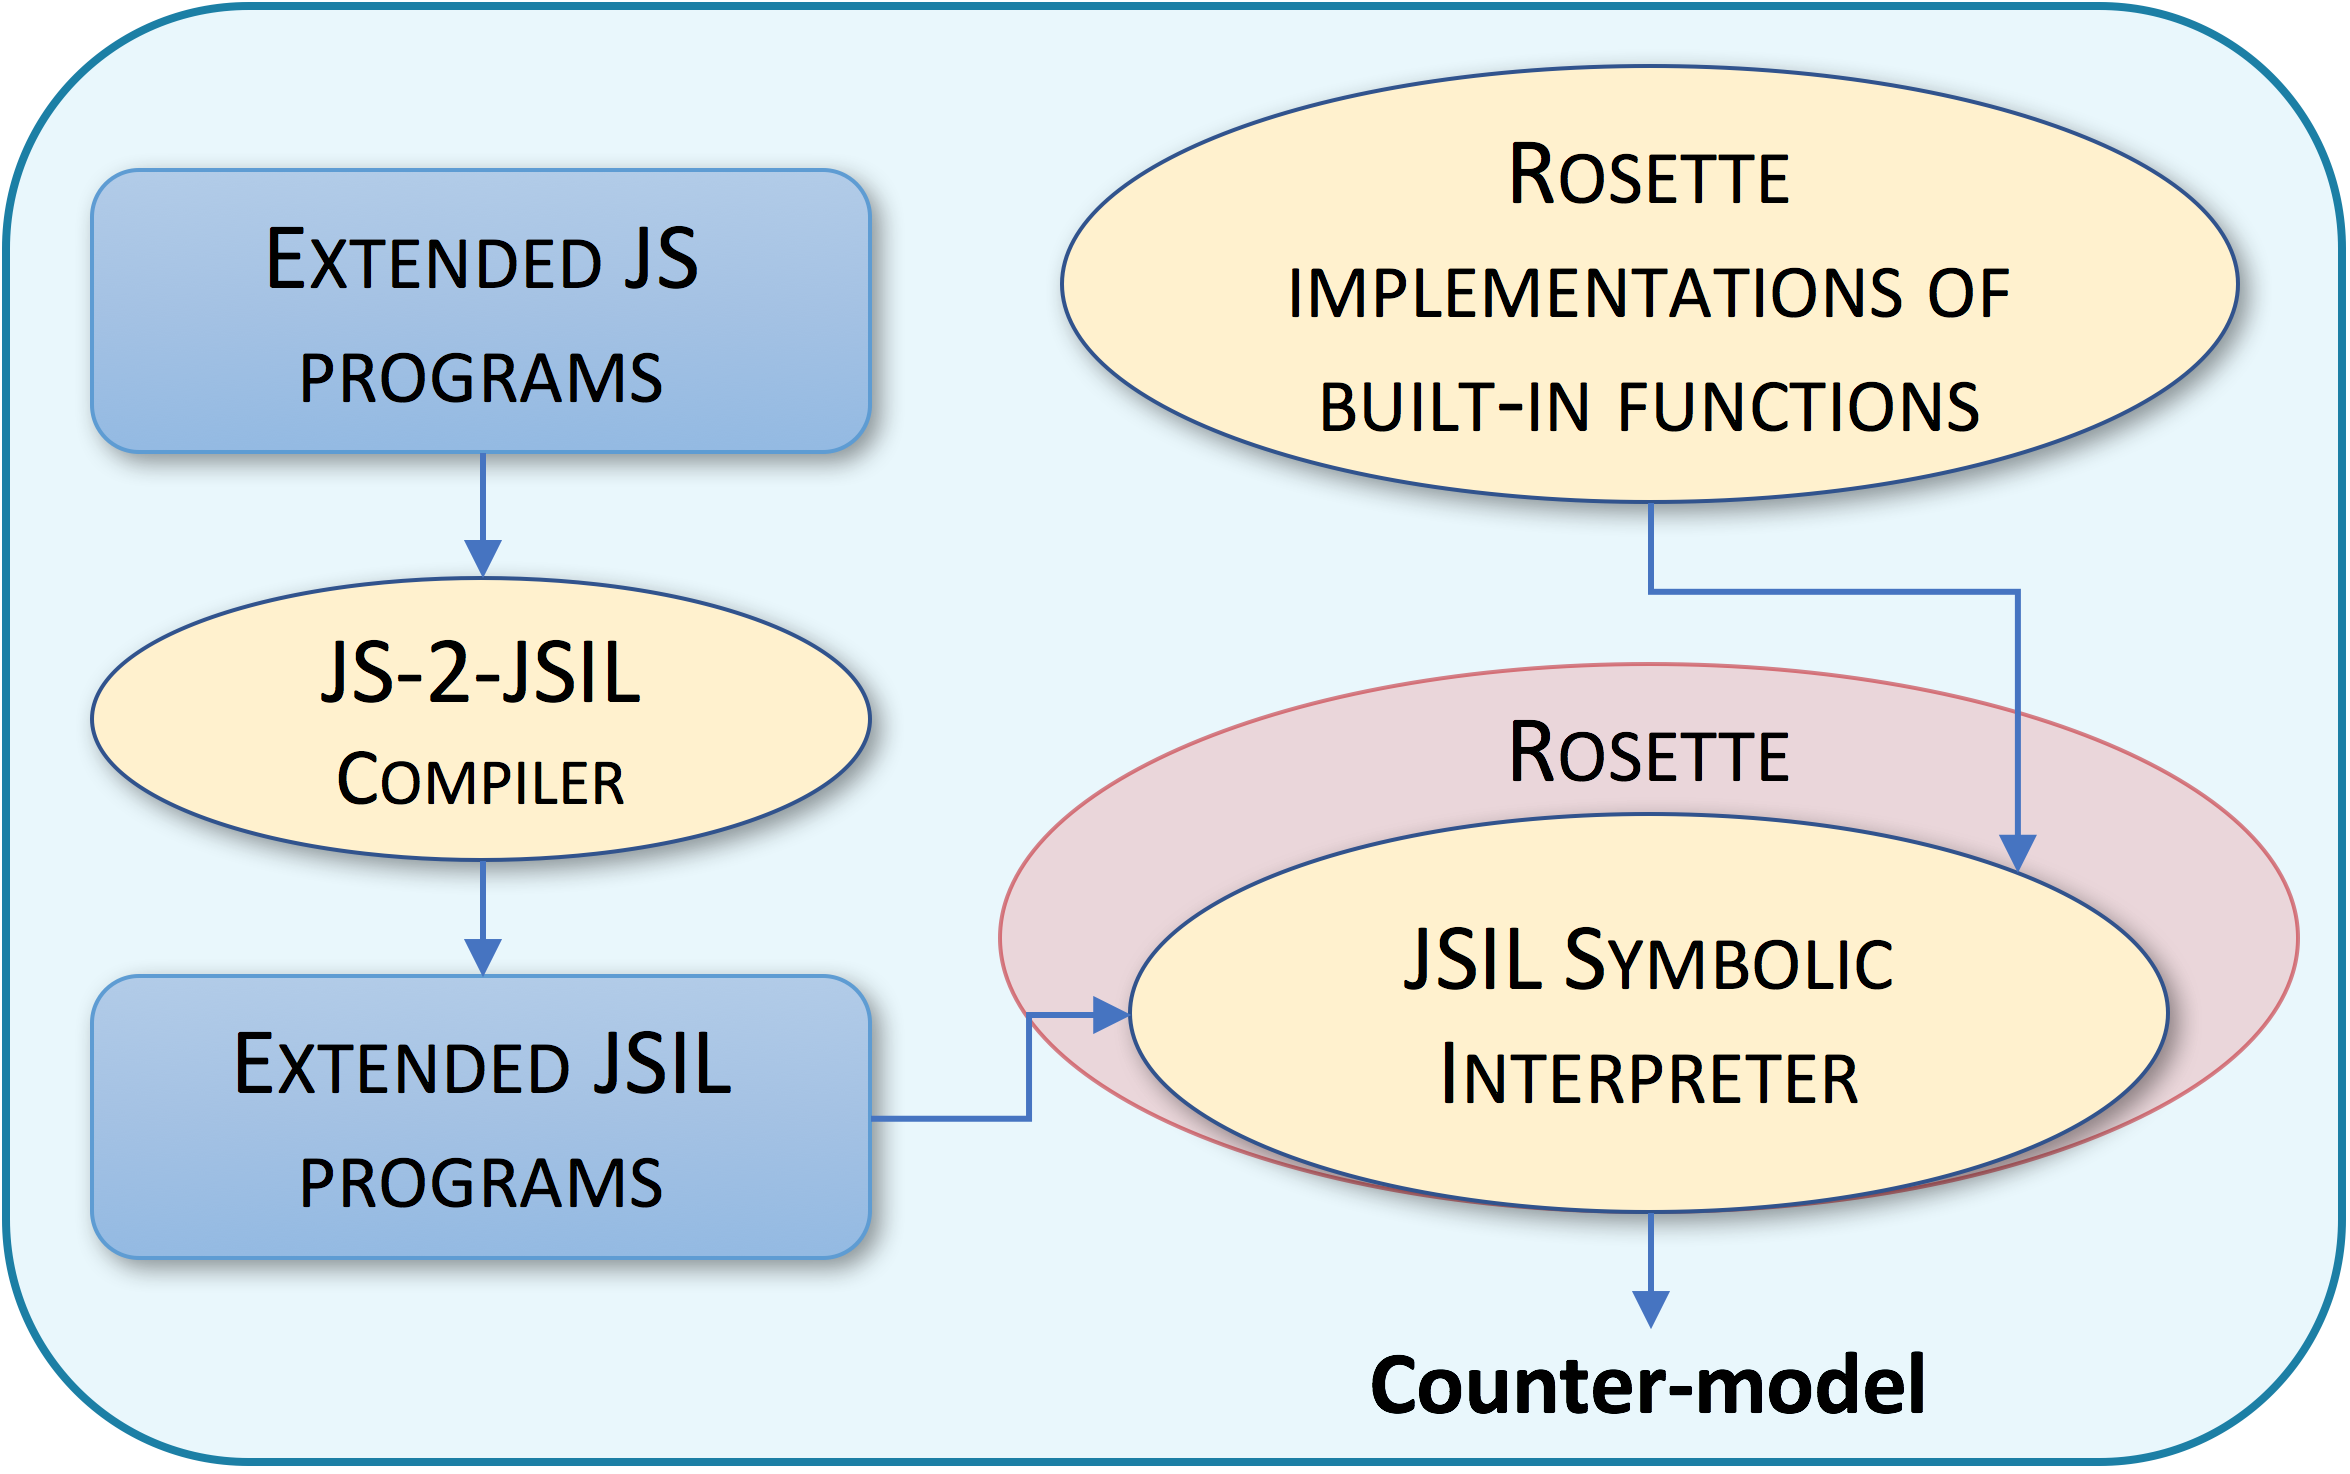
\includegraphics[width=0.26\textwidth]{figures/jilette_blue.png}
\vspace*{-0.55cm}
\label{fig:jilette:diagram}
\end{wrapfigure}

The architecture of \cosette is shown on the right. We extend JavaScript with constructs for creating and reasoning about symbolic values. Using \JSComp~\cite{javert}, a trusted compiler from JS to the \jsil intermediate language, we compile the extended JS program to an extended \jsil program. The core of \cosette is a new symbolic interpreter for
\jsil,  written in 
Rosette~\cite{Rosette2,Rosette1}, a framework for creating
symbolic interpreters. The 
JSIL symbolic interpreter either outputs a concrete counter-model for the given assertions, or guarantees correctness up to a given bound for unfolding loops and recursive~predicates. %\pmaxinline{This is the first time we mention `bound'.}


%comprises a
%simple extension of \JSComp~\cite{javert}, a trusted compiler from 
%JavaScript to the \jsil intermediate language, to account for symbolic values and
%assertions, and a new symbolic interpreter for JSIL, implemented using
%Rosette~\cite{Rosette2,Rosette1}.  
%The JSIL symbolic interpreter 
%either outputs a concrete counter-model for the given assertions, or
%guarantees correctness up to a given bound for unfolding loops and
%predicates.  %\pmaxinline{This is the first time
%                                %we mention `bound'.}
                  
%\pmax{Now, get rid of JS-2-JSIL. Lifting}  
            
Our new, general methodology underpinning the compositional JSIL symbolic
interpreter consists of three stages: \dtag{1}~we design an JSIL
instrumented semantics that exhibits the frame property by explicitly
keeping track of object properties that we know are {\em not present}; 
\dtag{2}~we define
the JSIL symbolic semantics by lifting the JSIL instrumented
semantics; and \dtag{3}~we link the JSIL symbolic semantics to the
JSIL concrete  semantics by describing the frames that can be safely
added to the initial state.
%
%Much like JavaScript, \jsil does not exhibit the frame property~\cite{reynolds:lics:2002}, raising the issue of how to guarantee that the results of the analysis still hold when extending the initial state of the analysed program with a given arbitrary frame.
The key innovation is to have the instrumented semantics as a proper
interim stage in the design of the symbolic execution, obtaining more modular
reasoning and substantially simpler proofs. We present this methodology  in~\S\ref{sec:jsil:symb:exec}. 








%We extend the syntax of JavaScript with constructs
%for creating and reasoning about symbolic values, which allow the
%developer to easily write assertions about the behaviour of their
%program. Using \JSComp, we compile the extended JS program to an
%extended \jsil program. The core of \cosette is a symbolic interpreter
%for \jsil, 



%%how do we do it


%Cosette depends on a new methodology, presented here, for designing compositional
%program analyses for languages that do not exhibit the frame property.
%
%For Cosette, the methodology is applied to JSIL, which like JavaScript
%does not satisfy the frame property. 




%\pgmaxinline{In section 3, just mention methodology, then immediately get on to
%  the abstract semantics, which is the key additional technical point
%  that I'm not mentioning in the introduction. Basically, most of para
%1 is out because given here.} 








%in that it comes with formal correctness guarantees and a \polish{result stating the precise conditions under which symbolic execution gives soundness}. 


An essential goal for us was to establish trust in Cosette. In
\S\ref{sex:formal:guarantees}, we give a {\em bounded soundness
  result} for the \jsil symbolic semantics and prove that \cosette
never produces false positive bug reports. These theoretical results,
combined with the correctness of the \JSComp compiler~\cite{javert}
and the fact that the memory models of JavaScript and \jsil are the
same by design, enable us to lift the results of analyses done on
compiled \jsil code back to the original JavaScript code
(cf.~\S\ref{subsec:liftmejs1}, \S\ref{subsec:liftmejs2}). We must also
establish trust in the Cosette implementation. 
We  implement the \jsil  instrumented interpreter following the \jsil 
instrumented semantics of \S\ref{subsec:instrumented} to the letter.
We test the combination of the 
JS-2-JSIL compiler and the \jsil instrumented  interpreter using Test262, 
the official ECMAScript test suite~\cite{test262}. Out of the
10469 tests for ES5 Strict, we identify 8330 tests appropriate
for our coverage, of which we pass 100\%.
Finally, we ensure that the \jsil symbolic interpreter obtained by the 
Rosette lifting of the \jsil instrumented interpreter is consistent 
with the symbolic semantics of \S\ref{subsec:symb:semantics}
by systematically constructing symbolic unit tests for each \jsil command,
assuming the premises and asserting the conclusion of the 
appropriate rule of the symbolic~semantics. 


%We also created a number of symbolic tests specifically to demonstrate that Cosette can reason about essential JavaScript features, such as prototype inheritance, function closures, arrays, strings, as well as the substantially more challenging for-in statement and dynamic dispatch.


%\pgmaxinline{Not finished trust, next bits might be useful.} 

%The main issue with most bug-finding tools is not that they are not sound, but that they are not \emph{trustworthy}: the extent of their soundness and precision is not formally characterised. They are usually not justified with respect to the semantics of the targeted language, often relying on unstated simplifying assumptions, if not explicitly departing from the semantics. Consequently, the fact that a bug-finding tool cannot find a bug carries no guarantees whatsoever with respect to the correctness of the input program. We trust these tools because they appear to work empirically. 

%The current approaches~\cite{.} normally do not give a formal account of the analysis and/or simplify the language semantics. Our approach to designing \cosette is grounded on adherence to the standard and establishing trust. 




%We move the analysis to \jsil, an intermediate representation for logic-based analysis of JavaScript, which comes with a trusted compiler, \JSComp~\cite{javert}.
%, which has been extensively tested against the official test suite, Test262.\footnote{\url{https://github.com/tc39/test262}} 
%and produces \jsil code that corresponds line-by-line to the
%standard. 





%In \S\ref{sec:jsil:symb:exec}, we give a novel abstract semantics for \jsil, which we instantiate to obtain the concrete and symbolic semantics, connected via a {\em bounded soundness result}. Moreover, we prove that \cosette is precise, meaning that it never produces false positive bug reports. 
%These theoretical results, combined with the correctness of \JSComp and the fact that the memory models of JavaScript and \jsil are the same by design, 
%allow us to  provably lift the results of analyses done on compiled
%\jsil code back up to JavaScript (\S\ref{sec:lifting}). %To our
                                %knowledge, this is the first
                                %formalisation of a symbolic execution
                                %used for JavaScript analysis, and is
                                %the first symbolic execution for
                                %JavaScript that precisely follows the
                                %semantics of the language.


%\pgmaxinline{The bit on trustworthyness in section 5 can be shortened. Readers need to be reminded what was said in intro,  that's all. I do think there should be a proper evaluation of  Cosette coverage in evaluation. We can do whole-program analysis up  to the coverage point.}


%\pgmaxinline{This next bit can be shortened, to dovetail with section 2 which is also on application. For each applciation, update the evaluation to match what you do in 5} 





We apply Cosette to whole-program symbolic testing. 
A general developer can use \cosette for symbolic testing of
their code by having symbolic inputs instead of concrete
inputs and stating the constraints that the output needs to satisfy as
simple, intuitive first-order assertions over these inputs. If
a test fails, \cosette provides the concrete input that causes it to
fail, exposing bugs in the tested code. In \S\ref{sec:evaluation}, 
we evaluate \cosette on two real-world JavaScript data structure libraries,
where, using fewer tests, we achieve better coverage (100\%) than
the concrete unit test suites shipped with the libraries, and
discover unexpected bugs in both libraries.


%: Buckets.js [? ] with 65k downloads on
%npm~\cite{.}, and queue-pri [? ]. We found a significant bug in both
%libraries, and obtained 100\% coverage with fewer symbolic tests.
%
%and provide a detailed evaluation in~\S\ref{sec:evaluation}



%In \S\ref{sec:evaluation}, we evaluate \cosette on challenging
%real-world examples that showcase JS-specific features, as well as on real-world Node.js libraries, in which we discover several~bugs. 


We also apply Cosette to specification-driven bug-finding. 
%\pmaxinline{Feeling stuck here.} 
%Due to the complexity of JavaScript semantics, 
Full functional correctness 
specifications of JavaScript programs are highly intricate, with only
a few tools (mainly, \javert~\cite{javert} and KJS~\cite{Park:2015,stefanescu:oopsla:2016}) supporting such expressivity. 
%They target the specialist developer wanting rich, mechanically verified specifications of critical JavaScript code.
When these tools cannot prove that a given function satisfies
a specification, the specialist developer needs to
understand in detail a complicated proof trace to discover the error. 
% (\javert), or act with essentially no feedback~(KJS). 
In \S\ref{subsec:sdbf}, we show how
\cosette can be used as an auxiliary mechanism for debugging
separation logic specifications of JavaScript programs in \javert.
This application of Cosette is possible due 
to its compositionality.
Our approach, described in detail in \S\ref{sec:specs}, consists of
translating the separation logic specifications into symbolic tests
and running these tests using \cosette.  Then, if a symbolic test
generated from a given specification fails, we can be sure that the
code to be verified does not satisfy its specification.  More
importantly, \cosette then generates a concrete witness that
invalidates the specification. This information greatly simplifies the
debugging of both specifications and code.

%%how we do it


%\pgmaxinline{Next para probably in conclusions, it's all about next
%  steps.} 
%
%
%Because it is trustworthy, \cosette can be used both as a basis for building other more specific analysis 
%\polish{(I can talk about the analysis that Peter Thieman wants to write)} and 
%as a testing oracle for other symbolic execution tools for JavaScript that purposely 
%ignore some corner cases of the language semantics. 
%\polish{No previous symbolic execution tool for JavaScript came with the frame resilience result. 
%None of them can be used to test JS specs.}



%
%Symbolic testing provides an analysis of whole program behaviour. It
%works well for static languages such as C and Java which satisfy the
%{\em frame property}. Intuitively, the frame property states that, if
%a program produces an output when run in a given state, then it will
%produce the same output when run in an extended state. With the frame
%property, testing a C or Java program with respect to a symbolic state
%guarantees that the program will behave in the same way when the state
%is extended arbitrarily.  Symbolic testing works less well for dynamic
%languages such as JavaScript which do not satisfy the frame property.
%Without the frame property, testing a JavaScript program with respect
%to an initial symbolic state does not guarantee that the program will
%behave in the same way when the state is extended.  Such whole-program
%analysis is therefore not the best fit for JavaScript applications,
%which are commonly run in highly dynamic execution environments
% where the state can be extended  arbitrarily. 
%
%
%
%%%what is our solution: compositionality
%
%
% We introduce {\em compositional} symbolic testing for JavaScript
% programs by working with partial instrumented symbolic heaps.
% Compositionality is acheived by providing instrumentation that
% explicitly keeping track of properties that must {\em not be present}
% in a given partial heap in order for the program to behave correctly.
% The operational semantics of JavaScript over such instrumented heaps does satisfy the frame
% property.  
%
%,,,,,
%
%
%
%
%
%
%
%instrumentation needed for frame. 
%
%spec-driven bug finding and compositional symbolic testing. 
%
%
%%%trustworthiness
%
%
%
%
%%%%%%evaluation of the tool
%
%We are doing compositional symbolic execution  for JavaScript 
%applications to whole-program symbolic testing, specification-driven
%bug finding and whatever else you've talking about 
%
%
%Moreover, the compositionality of \cosette allows us to catch bugs that are not reachable by standard symbolic execution tools.
%We illustrate the capabilities of \cosette on an array of examples, which include tests from the Test262 test suite and real-world Node.js libraries, and which make use of JavaScript-specific features, such as prototype inheritance, function closures, the for-in statement, and dynamic dispatch. \pmaxinline{Revisit after evaluation.}
%
%
%



%---------------THE OLD INTRO-----------------------

%\pmax{What is the reader supposed to learn?}






%In current program analysis research, there exists a gap between bug-finding techniques and verification techniques. Bug-finding discovers concrete executions that cause a given program to behave incorrectly, emphasising precision, that is, the absence of false positives. Verification produces proofs that a given program \emph{always} behaves correctly, emphasising soundness, which mandates adherence to the language standard and  exploration of all possible paths.
%
%Achieving soundness, however, is difficult and often costly, resulting in prohibitive scalability issues. In fact, most modern analysis applications, including bug-finding tools, have various intended and/or unintended sources of unsoundness~\cite{soundyPaper}.
%
%\polish{There is a growing consensus among experts that soundness is,
%in fact, not a necessity for most modern analysis
%applications~\cite{.}. Instead, the property they advocate and
%observe in the  majority of tools is \emph{soundiness}---maintaining
%soundness as much as possible, but without detrimental effects to
%precision and/or scalability.}


%Additionally, its compositionality allows us to catch a broader class of bugs than the current symbolic execution tools and also allows us to state the conditions under which the soundiness of \cosette becomes soundness, that is, when the absence of found bugs implies verification.

%However, compositionality is not trivial to achieve when the targeted programming language does not exhibit the frame property, as is the case for most dynamic languages including JavaScript.




%JavaScript is the most widespread dynamic language: it is the de facto language for client-side Web applications, used by 94.8\% of websites\footnote{\url{https://w3techs.com/technologies/details/cp-javascript/all/all}}; it is used for server-side scripting via Node.js; and it is even run on small embedded devices with limited memory. 
%It is the most active language in both GitHub and StackOverflow.\footnote{\url{http://githut.info}; \url{https://exploratory.io/viz/Hidetaka-Ko/94368d12800a?cb=1469037012628}}
%Due to its dynamic nature and complex semantics, JavaScript remains a difficult target for symbolic analysis and logic-based verification. 

%\pmax{Now, sth about the state-of-the-art}

% TO RELATED WORK
%Currently, several symbolic analysis tools for JavaScript are available, such as \pmaxinline{list them, cite them - are we doing static or dynamic also?}. \pmaxinline{Say something positive, don't know what, mention bug-finding}. However, there exists a gap that needs to be addressed. The symbolic analysis engines of these tools are not formalised and do not come with correctness guarantees \pmaxinline{check, especially Jalangi}. Their analyses are also not compositional \pmaxinline{We don't know what this means yet, also check, but possibly omit}. Moreover, each of these tools is tailored for catching a specific category of bugs, rather than targeting bug-finding in general \pmaxinline{give evidence - also, why do we care?}.



%We evaluate \cosette on an array of examples, including tests from the official JavaScript Test262 test suite and real-world Node.js libraries. These examples involve JavaScript-specific features, such as prototype inheritance, function closures, the for-in statement, and dynamic dispatch. We highlight the range of \cosette by using it to find bugs in a number of non-trivial separation logic specifications of JavaScript programs.



%In \S\ref{???}, we give an abstract semantics of \jsil, which we instantiate to obtain the concrete %, instrumented (discussed shortly), 
%and symbolic semantics, connected via a {\em soundness result}. Moreover, we prove that, when used for symbolic testing (discussed shortly), \cosette never produces false counter-models. 
%These theoretical results, combined with the correctness of \JSComp, allows us to lift the results of analyses done on compiled \jsil code back up to JavaScript. 

%To our knowledge, this is the first formalisation of a symbolic execution used for JavaScript analysis, and is the first symbolic execution that precisely follows the semantics of the language.
 



%
%Current symbolic execution tools for JavaScript~\cite{???} are not compositional. They assume access to the entire program, meaning that the results they obtain when analysing functions in isolation cannot be reused, as they would not account for the interaction between the function and all of its possible frames.
%
%In contrast, the symbolic execution of \cosette is compositional. This has several important benefits.
%
%First, it allows us to use function specifications instead of symbolically executing function bodies at each call site, speeding up execution time. This benefit is independent of the analysed language.
%
%Next, it allows us to catch frame bugs, which are not reachable by non-compositional symbolic execution tools. This benefit is specific to dynamic languages.
%
%Finally, it allows us to state a verification result for \cosette, precisely capturing the conditions under which our symbolic execution is sound.
%
%, meaning that once a program is analysed successfully, once can choose to re-use the results of the analysis when analysing code that calls it, also yielding a more scalable analysis.
 

%The second component that \cosette uses is \JSComp~\cite{javert}, 
%a well-tested, standard-compliant compiler from JavaScript to \jsil. We extend
%\JSComp with support for the non-strict mode of ES5, as well as
%regular expressions and the entire \jsinline|String| built-in library.
%\JSComp allows us to lift the \jsil symbolic execution to JavaScript by first compiling JavaScript code to \jsil code, and
%then symbolically executing the compiled code in the 
%\jsil symbolic interpreter. This process, described in \S\ref{symb:exec:comp},
%involves extending JavaScript syntax and the \JSComp compiler to support symbolic values and 
%constructs for reasoning about them. These constructs are intuitive
%and allow the general developer to easily write assertions about the behaviour
%of their program. 
%Moreover, we adjust the \jsil symbolic interpreter so that the abstraction level 
%of the generated \jsil code precisely matches the abstraction level of Rosette, 
% maximising the use of Rosette's native reasoning capabilities.

%dynamic languages: they feature extensible objects, dynamic property access, and dynamic function calls. In terms of separation logic, they do not have the frame property~\cite{???}. What this effectively means is that is possible to introduce bugs into a JS/\jsil program by only extending the state for which it behaved correctly. We refer to such bugs as {\em frame bugs}.  This benefit is independent of the analysed language. Second, it allows us to catch frame bugs, which are not reachable by non-compositional symbolic execution tools. This benefit is specific to dynamic languages. We achieve compositionality by keeping track of properties that we know are {\em not present} in a given object. This we describe in detail in \S\ref{???}. To our knowledge, \cosette is the first compositional symbolic execution tool for dynamic languages.



%\myparagraph{Overview} 
%In \S\ref{sec:overview}, we illustrate how \cosette can be used for symbolic testing and specification-directed debugging of JS code. In~\S\ref{sec:jsil:symb:exec}, we present our methodology for the design of program analyses for dynamic languages and give a detailed account of our symbolic execution for \jsil. Our experimental evaluation of \cosette is given in . Finally, in \S\ref{sec:rwc}, we discuss related work and give conclusions.


%\pmax{Say more clearly what the novelty is. Say in a very pretty way the connection between seplogic and non-seplogic, verification and symbolic execution, etc.}

%We highlight two relevant use cases for \cosette. First, we show how \cosette can be used as \dtag{i}~a tool for running symbolic tests for JavaScript programs; and \dtag{ii} a debugging tool for separation logic specifications of JavaScript programs.

%\myparagraph{Architecture}
%The core of \cosette consists of a symbolic interpreter for
%\jsil~\cite{javert}, a simple intermediate goto language. 
%We obtain this symbolic interpreter \emph{for free}, 
%by implementing a concrete \jsil interpreter in Rosette~\cite{Rosette2,Rosette1},~a 
%symbolic virtual machine that facilitates generation of solver-aided languages.
%We design the concrete interpreter so that all of Rosette's natively supported solver-aided features, such as advanced string and regular-expression reasoning, 
%are lifted to the \jsil symbolic interpreter. 
%In~\S\ref{sec:jsil:symb:exec}, we give a formalisation of the \jsil concrete and symbolic executions, linking them together with a {\em soundness result}. We also provide insights on how to correctly design the concrete \jsil interpreter in Rosette.

%The second component that \cosette uses is \JSComp~\cite{javert}, 
%a well-tested, standard-compliant compiler from JavaScript to \jsil. We extend
%\JSComp with support for the non-strict mode of ES5, as well as
%regular expressions and the entire \jsinline|String| built-in library.
%\JSComp allows us to lift the \jsil symbolic execution to JavaScript by first compiling JavaScript code to \jsil code, and
%then symbolically executing the compiled code in the 
%\jsil symbolic interpreter. This process, described in \S\ref{symb:exec:comp},
%involves extending JavaScript syntax and the \JSComp compiler to support symbolic values and 
%constructs for reasoning about them. These constructs are intuitive
%and allow the general developer to easily write assertions about the behaviour
%of their program. 
%Moreover, we adjust the \jsil symbolic interpreter so that the abstraction level 
%of the generated \jsil code precisely matches the abstraction level of Rosette, 
% maximising the use of Rosette's native reasoning capabilities.

%\myparagraph{Application: Symbolic Testing} A commonly used 
%approach to obtaining trust in JavaScript code is running it against 
%adhoc test batteries---verifying that given concrete inputs, the code produces the expected
%output. The main drawback of this approach is that tests, in general,
%cannot guarantee exhaustiveness. % we also cant guarantee exhaustiveness 
%In \S\ref{symbolic:testing}, we show how to use \cosette
%for symbolic testing of JavaScript code: instead of 
%tests with concrete 
%inputs, the developer uses symbolic inputs and states the 
%constraints that the output needs to satisfy as simple, intuitive 
%first-order assertions over these inputs. 
%Furthermore, if a test fails, \cosette provides the concrete inputs that cause it 
%to fail, exposing bugs in the tested code. 
%We highlight the capabilities of \cosette through examples that showcase
%challenging reasoning on strings, regular expressions, and the \jsinline|eval|
%statement.

%\myparagraph{Application: Debugging Separation Logic Specifications}
%Due to the complexity of JavaScript semantics, functional correctness 
%specifications of JS programs are highly intricate. 
%There are only a few tools (for example, \javert \cite{javert} and KJS \cite{Park:2015,stefanescu-park-yuwen-li-rosu-2016-oopsla}) that support such expressivity. They target the specialist developer wanting rich, 
%mechanically verified specifications of critical JavaScript code.
%However, when these 
%tools cannot prove that a given function satisfies a specification, to discover the error, 
%the developer needs to understand in detail a complicated proof trace (\javert), or even act with almost no feedback~(KJS). 
%
%In \S\ref{sec:specs}, we show how \cosette can be used as an auxiliary mechanism for debugging 
%separation logic specifications of JavaScript programs in \javert. 
%Our approach consists of: translating the separation logic specifications 
%into symbolic tests 
%and running these tests using \cosette. 
%Then, if a symbolic test generated from a given specification fails, we can 
%be sure that the code to be verified does not satisfy its specification. 
%More importantly, \cosette then generates a concrete witness that 
%invalidates the specification. This information greatly simplifies the debugging of 
%both specifications and code. 

%Jilette has the following benefits: 
%
%\dtag{1} it is \emph{useful}, in that it has tangible applications:
%	it can report bugs in JavaScript programs, producing concrete witnesses that trigger these  bugs; 
%	%
%	it can be used as a helper tool for developers of logic-based functional correctness specifications of JavaScript code; 
%	%
%	and it has support for advanced string reasoning, critical for reasoning about commonly used JavaScript code;
%
%\dtag{2} it is \emph{accessible}, in that it can easily be used by a general JavaScript developer: 
%	the annotation burden of \cosette is minimal; 
%	%
%	and the assertion language is simple and intuitive;
%\dtag{3} it is \emph{trustworthy}, in that its components come with correctness guarantees: 
%	the correctness of the \JSComp compiler ensures full adherence to the real semantics of JavaScript;
%	%
%	the soundness result for the symbolic execution used in \cosette guarantees absence of false positives;
%	and \polish{sentence about unification;}
%and \dtag{4} it is \emph{extensible}, in that its coverage can easily be extended in a modular way, allowing support for: 
%	built-in libraries not covered by \JSComp; 
%	%
%	and widely used runtime libraries that are not part of the standard, such as the DOM.

%\pmax{What's the story?
%\begin{enumerate}
%\setlength{\itemsep}{0.5em}
%\item 
%	{\bfseries Slogan}: Symbolic execution for JavaScript that precisely follows the language standard. \\ 
%	{\bfseries Goal}: Symbolic testing, bug-finding, concrete counter-models. \\
%	{\bfseries Novelty}: The precision wrt semantics, formal correctness guarantees. \\ 
%	{\bfseries Benefits}: Trustworthy, sound analysis. \\
%	{\bfseries Limitations}: No loop invariants, bounded. No eval.
%
%\item 
%	{\bfseries Slogan}: Compositional execution for dynamic languages in general, and JavaScript in particular. \\ 
%	{\bfseries Novelty}: Compositionality. \\ 
%	{\bfseries Benefits}: summaries, frame-related bugs.   
%	
%\item 
%	{\bfseries Application}: Symbolic testing of JavaScript programs. \\
%	{\bfseries Novelty}: None? \\ 
%	{\bfseries Evaluation}: Tests for the symbolic execution rules; JS programs using prototype inheritance, arrays, function closures, for-in, dynamic dispatch, etc.; test262 tests; node.js libraries for data structures
%	
%\item 
%	{\bfseries Application}: Debugging of separation logic specifications. \\ 
%	{\bfseries Novelty}: Counter-models for separation logic assertions. \\
%	{\bfseries Evaluation}: JaVerT specifications of this and that.
%\end{enumerate}}




%
%\myparagraphq{Why \cosette} 
%\cosette is \emph{useful}: it has tangible applications. 
%It can report bugs in JavaScript programs, producing concrete witnesses triggering the bugs. It can also be used as a helper tool for developers of logic-based functional correctness specifications of JavaScript code.
%\cosette is \emph{approachable}: it can easily be used by a general JavaScript developer. The annotation burden of \cosette is minimal and the assertion language is simple and intuitive. \polish{Sweet spot?}
%\cosette is \emph{trustworthy}: its components come with correctness guarantees. 
%The correctness of the \JSComp compiler ensures full adherence to the real semantics of JavaScript. The \cosette symbolic execution engine is based on a sound symbolic
%analysis for \jsil, guaranteeing the absence of false positives. \polish{Sentence about unification.}
%Finally, \cosette is \emph{extensible}: its coverage can easily be extended in a modular way. This gives us the mechanism for supporting built-in libraries not covered by \JSComp, or adding support for standard-external runtime libraries, such as the DOM.




%\newpage
%
%\myparagraph{What's in the paper}
%
%\bigskip
%\polish{TO GO IN SOMEWHERE \\
%
%Clarify ES5 Strict
%
%JaVerT targets the specialist
%developer wanting rich, mechanically verified specifications of critical JavaScript code.
%Functional correctness, yes, and it works, but paid for by a heavy annotation burden.
%}



%We show how  to use Jilette for writing symbolic tests for client side 
%JavaScript code calling Web APIs. In particular, we demonstrate how to 
%checking the conformance of Web API requests with their specified signatures. 
%The existing solutions for this problem are still imprecise due to the 
%dynamicity of JavaScript combined with the difficulty of reasoning about
%operations on symbolic strings \cite{Idontknow}. Jilette is an excellent fit for
%this task as it leverages on Rosette's back-end
%constraint solver, Z3, which supports reasoning on symbolic strings
%and regular expressions, whereas JS-2-JSIL successfully
%contains the complexity of JavaScript itself.

\section{Using \cosette}\label{sec:overview}
%!TEX root = ../main.tex

We illustrate how \cosette can be used both for whole-program and compositional symbolic testing of JavaScript programs. We demonstrate how \cosette  explicitly exposes the resilience of JavaScript programs to the environment, not considered by standard symbolic execution tools, but essential for compositional analysis.

 \begin{figure*}[t]
 \centering
 %
 \begin{subfigure}[b]{0.33\textwidth}
 {\lstset{language=JavaScript,basicstyle=\fontsize{7}{7}\ttfamily,escapeinside={~}{~}}
 \begin{lstlisting}
function Map () { this._contents = {} }

Map.prototype.get = function (k) {
  var c = this._contents;
  if (this.validKey(k)) {
    return (c.hasOwnProperty(k) ? c[k] : null)
  } else throw new Error("Invalid Key");
}

Map.prototype.put = function (k, v) {
  if (this.validKey(k)) {  
    this._contents[k] = v   
  } else throw new Error("Invalid Key");
} 

Map.prototype.validKey = function (k) { ... }
\end{lstlisting}}
\vspace*{-0.2cm}
\caption{Library implementation}
\label{fig:2a}
\end{subfigure}
%
 \begin{subfigure}[b]{0.33\textwidth}
 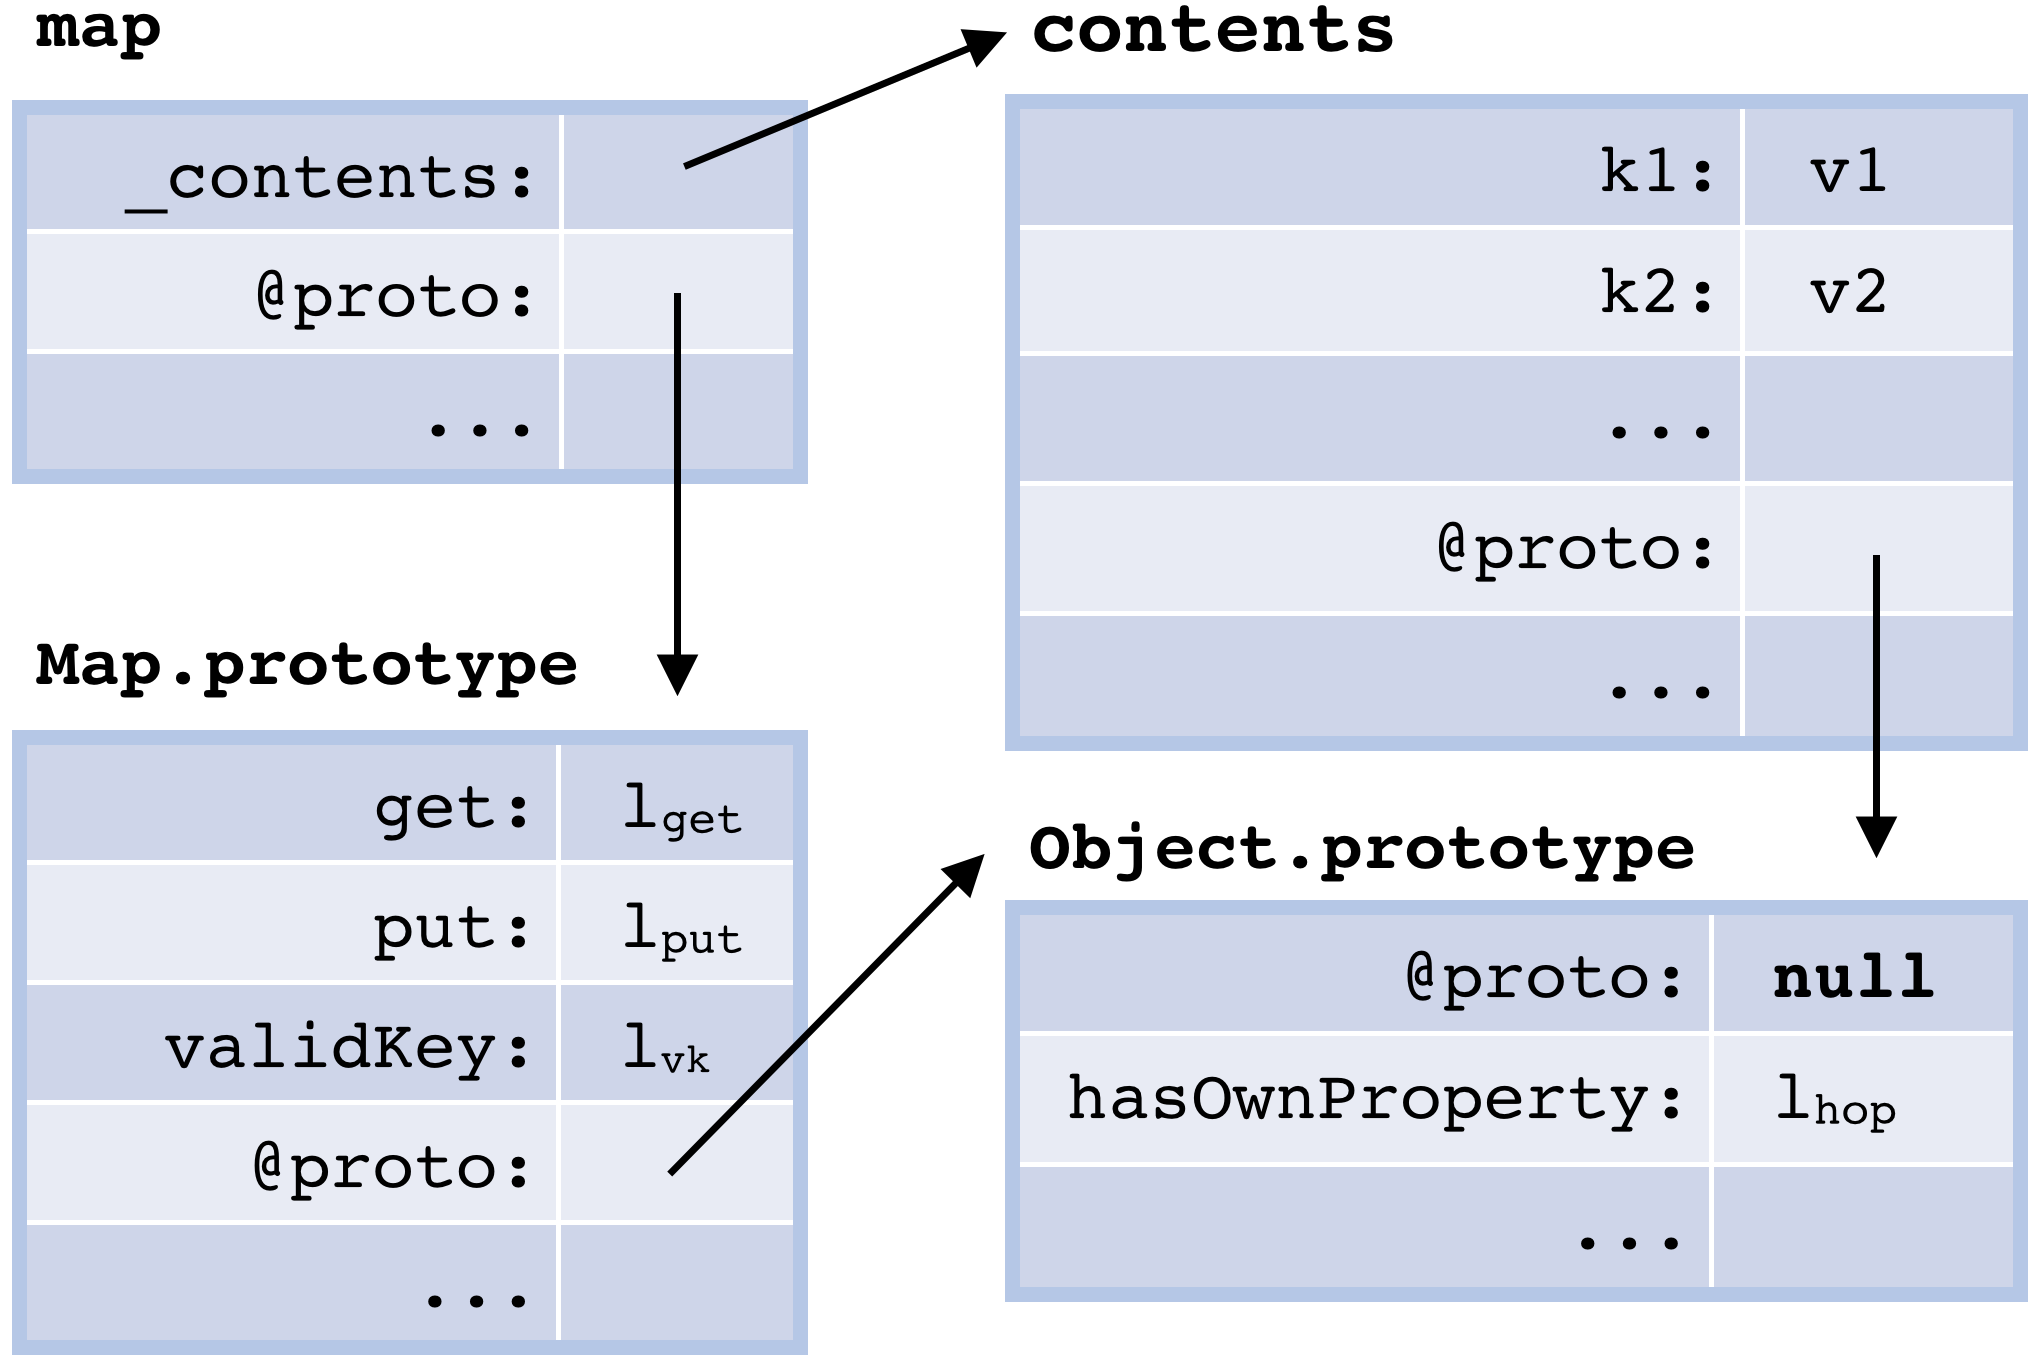
\includegraphics[width=0.93\textwidth]{figures/mapDiagram.png}
 \vspace*{0.5cm}
 \caption{General library heap}
 \label{fig:2b}
 \end{subfigure}
 %
 \begin{subfigure}[b]{0.3\textwidth}
 \centering 
 {\lstset{xleftmargin=.17\textwidth,language=JavaScript,basicstyle=\fontsize{7}{7}\ttfamily,escapeinside={~}{~}}
\begin{lstlisting}
var k = symb_string();
var v = symb_number();
assume(validKey(k));
var m = new Map(); m.put(k, v); 
var result = m.get(k);
assert(result = v)
\end{lstlisting}}
\vspace*{0.1cm}
 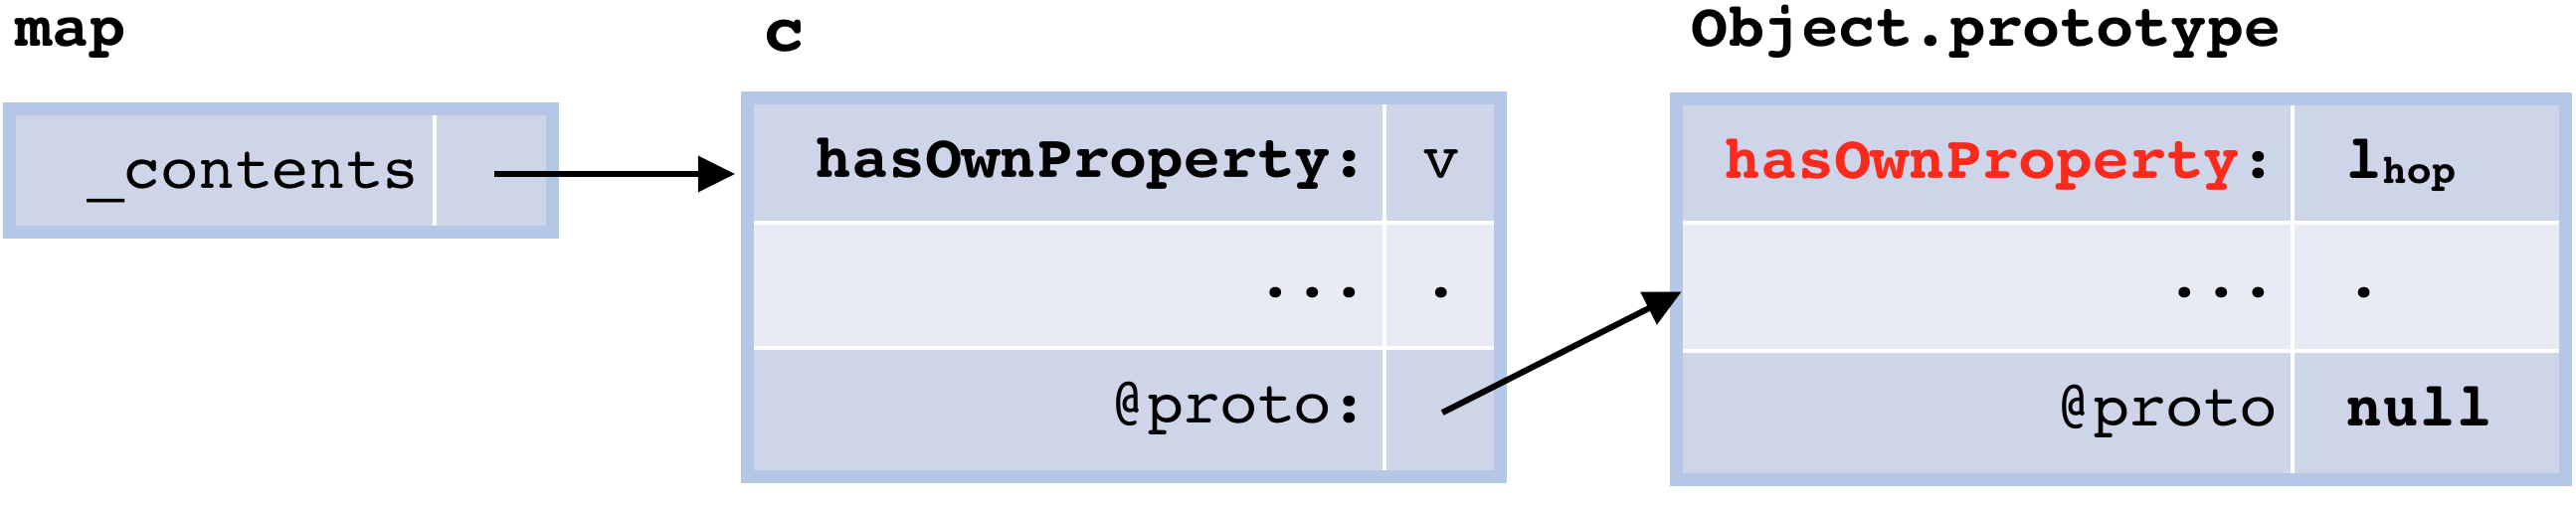
\includegraphics[width=0.78\textwidth]{figures/heapfail.png}
 \captionsetup{format=nastyCaption}
\caption{Simple symbolic test (above); \\the \jsinline|"hasOwnProperty"| bug (below)}
\label{fig:2c}
\end{subfigure}
\vspace*{-0.25cm}
\caption{Running example: JavaScript key-value map library}
\label{fig:two}
 \vspace*{-0.4cm}
\end{figure*}

Our running example is a \emph{key-value map} implementation, given in Figure~\ref{fig:2a}. It contains four functions: 
\jsinline|Map|, for constructing an empty map;
\jsinline|get|, for retrieving the value associated with a given key;
\jsinline|put|, for inserting/updating key-value pairs; and \jsinline|validKey|, for deciding whether or not a key is valid.
The map library implements a \emph{key-value map} as an object with property \jsinline|_contents|, denoting the object storing the map contents.  
The named properties of \jsinline|_contents| and their value attributes correspond to the map keys and values, respectively.
The functions \jsinline|get|, \jsinline|put|, and \jsinline|validKey| are shared between all map 
objects and are, therefore, defined in \jsinline|Map.prototype|, which is the prototype\footnote{In JavaScript, inheritance is modelled through \emph{prototype chains}. On property lookup, $\mathtt{o.p}$, we first check if the property $\mathtt{p}$ is present in the object $\mathtt{o}$, in which case its value is returned. Otherwise, we  check if $\mathtt{p}$ is present in the prototype of $\mathtt{o}$, and so  forth.} of all objects created using \jsinline|Map| as a constructor (i.e.,~using~\jsinline|new Map()|). 
The \jsinline|get| function returns the value associated with a given key in the map, or \jsinline|null| if the key is not in the map. 
Note that, in order to check that the given key is in the map, \jsinline|get| uses the built-in function \jsinline|hasOwnProperty|, which lives in \jsinline|Object.prototype|, the prototype of all objects.
The \jsinline|put| function updates the map if the supplied key is valid, and otherwise throws an error. 
The \jsinline|validKey| function describes the conditions under which a given key is valid. 

In Figure \ref{fig:2b}, we show a general heap of key-value maps. There is the \jsinline|map| object, with its \jsinline|_contents| property pointing to the \jsinline|contents| object and its prototype being \jsinline|Map.prototype|. There is the \jsinline|contents| object, which holds the key-value pairs, and whose prototype is \jsinline|Object.prototype|. There is the \jsinline|Map.prototype| object, which holds the \jsinline|get|, \jsinline|put|, and \jsinline|validKey| functions,\footnote{In JavaScript, functions are modelled as objects in the heap. As their structure does not add to this example, we only show the locations of the appropriate objects.} and whose prototype is also \jsinline|Object.prototype|. Finally, there is \jsinline|Object.prototype|, which holds the \jsinline|hasOwnProperty| function that is called by \jsinline|Map.prototype.get|.

%Observe that a naive implementation of the function \jsinline|validKey| may result in potential bugs. In particular, one can insert a key-value pair with \jsinline|"hasOwnProperty"| as a key into the map. By doing this, \jsinline|"hasOwnProperty"| in the prototype chain of \jsinline|_contents| is overridden and subsequent calls to \jsinline|get| will fail. 

%\myparagraph{Prototype chains and $\mathtt{Object.prototype}$}
%In order to better understand the implementation of the map library as well as its possible bugs, 
%one must first understand the \emph{prototype-based inheritance} mechanism of JavaScript. 
%Every JavaScript object has a prototype, which (for presentation purposes) we assume to 
%be stored  in an internal property \jsinline|@proto|. In order to determine the value of a property
%\jsinline|p| of an object \jsinline|o|, the semantics first checks if \jsinline|o| has a 
%property named \jsinline|p|, in which case the property look-up yields its value. Otherwise, the 
%semantics checks if \jsinline|p| belongs to the properties of the prototype of \jsinline|o| and so 
%forth. Hence, in the example, when looking up the value of the property \jsinline|hasOwnProperty|
%of the object \jsinline|contents|, one gets the value associated with the property  \jsinline|hasOwnProperty|
%of its prototype.
%The sequence of objects that can be accessed from a given object through the inspection 
%of the respective prototypes is called a \emph{prototype chain}.
%Prototype chains typically finish with the object \jsinline|Object.prototype| from which JavaScript 
%programs can access a number of built-in functions, which are part of the language runtime environment and are used for inspecting and manipulating objects.
%An example of such a function is \jsinline|hasOwnProperty(p)|, which checks whether or not the object 
%on which it is invoked has the property \jsinline|p| (e.g. {\small \jsinline|map.hasOwnProperty("_contents")|}
%evaluates to \jsinline|true| when evaluated in the heap shown in Fig.~\ref{map:example}-(right), 
%because the object \jsinline|map| has a property named~\jsinline|"_contents"|). 

\lstnewenvironment{lstjsex}{\lstset{language=JavaScript,basicstyle=\fontsize{8}{8}\ttfamily,escapeinside={~}{~}, numbers=none}}{}

\vspace*{-0.2cm}
\subsection{Whole-program Symbolic Testing}
\label{subsec:st}

Developers are used to writing unit tests for their code---verifying that, given some concrete inputs, the code produces the expected outputs. Using \cosette, they can write unit tests with \emph{symbolic} inputs and outputs, systematically testing a broad range of behaviours with a single symbolic test. For example, one meaningful unit test for the \jsinline|put| function consists of inserting a valid key-value pair \jsinline|(k, v)| into a map and then verifying that the pair has been inserted correctly. In Cosette, this test can be written as in Figure~\ref{fig:2c}. First, we declare \jsinline|k| to be a symbolic string and \jsinline|v| to be an symbolic number, using \cosette's constructs for creating symbolic variables. Next, we assume that \jsinline|k| is a valid key. Next, we create a new map, put the (symbolic) key-value pair \jsinline|(k, v)| into the map and then retrieve the value corresponding to the key~\jsinline|k|. Finally, we assert that the retrieved value is equal to the one we had previously put.

% 
When running \cosette on this test, if the \jsinline|validKey(k)| function was implemented incorrectly,\footnote{For instance, $\mathtt{validKey(k)}$ may only require that $\mathtt{k}$ is a string, which is a reasonable implementation, in the sense that it disallows JavaScript's implicit coercions.}
we will obtain the counter-model \jsinline|k = "hasOwnProperty"|. To understand this error, recall the heap and the implementation of \jsinline|get| from Figure~\ref{fig:two}. We can see that, if we were to put the key \jsinline|"hasOwnProperty"| into the contents object of a map, then the lookup of \jsinline|c.hasOwnProperty| done by \jsinline|get| will not reach \jsinline|Object.prototype| as intended, resolving instead to the \jsinline|hasOwnProperty| property of the \jsinline|contents| object (Figure~\ref{fig:2c}, below).

This example highlights how \cosette does not require specialist knowledge and can 
be used as a testing tool by a general JavaScript developer. The annotations amount to the creation of 
symbolic variables and the writing of assumptions and assertions, remaining minimal and intuitive, in contrast with the standard annotation burden of verification tools.

\vspace*{-0.2cm}
\subsection{Specification-driven Bug-finding}
\label{subsec:sdbf}

%\pmax{
%\begin{itemize}
%\item Compositionality = resilience to frame
%\item Summaries have to be resilient to frame
%\item BUT there are also NONES, and this is what is new
%\item Now guide through
%\item POINT - resilient to ALL frames, for whole-program analysis we are resilient only to one frame - we do get to create it, but it's only one after all
%\item Then, we can have more general specs, but needn't necessarily
%\end{itemize}
%}

As well as for whole-program analysis, \cosette can be used for compositional symbolic analysis of JavaScript functions in isolation, where the user specifies the functions in terms of their pre- and post-conditions. These specifications may account for only the parts of the heap required for running the function and can involve predicates, both recursive and non-recursive. We deal with recursive predicates by unfolding them to a  bound specified by the user.

Much like symbolic tests generalise concrete tests, specifications generalise symbolic tests. Given a JavaScript function, its specification, and the unfold depth for predicates, \cosette generates symbolic tests to verify that the function conforms to the specification up to that given depth. If this is not the case, \cosette will return a concrete counter-model that invalidates the specification. Unlike whole-program analysis tools, \cosette also tests if the given specification is compositional, that is, if it is resilient against all possible contexts in which the function can be run, and reports back to the user any found sources of non-compositionality.

\cosette supports the specification of symbolic states via simple separation logic assertions in the style of JaVerT~\cite{javert}. The developer has at their disposal a number of built-in predicates that capture the fundamental concepts of JavaScript (discussed throughout the text), and can define their own predicates as well. For instance, learning from the previous symbolic test, we could define the following predicate for describing valid keys:
\begin{Verbatim}[fontsize=\footnotesize,commandchars=\\\{\}]
    ValidKey(k) := types(k : Str) * (k <> "hasOwnProperty"),
\end{Verbatim}
\noindent meaning that \jsinline|k| is a valid key if it is a string that is not equal to \jsinline|"hasOwnProperty"|. From there, if we wanted to do a full functional correctness specification of the \jsinline|Map| library, we could, guided by the heap in Figure~\ref{fig:2b}, define the following two predicates:

% \textcolor{red}{(m, "get") -> None * (m, "put") -> None * (m, "validKey") -> None} * 
% * NoProps(c, keys)

\smallskip
\begin{Verbatim}[fontsize=\footnotesize,commandchars=\\\{\}]
 Map (m, mp, kvs) := JSObjectWithProto(m, mp) * 
   DataProp(m, "_contents", c) * JSObject(c) * KVPairs(c, kvs) * 
     \textcolor{red}{NoProp(m, "get")} * \textcolor{red}{NoProp(m, "put")} * \textcolor{red}{NoProp(m, "validKey")} * 
       \textcolor{blue}{NoProps(c, FProj(kvs))}
\end{Verbatim}
\begin{Verbatim}[fontsize=\footnotesize,commandchars=\\\{\}]
  KVPairs (c, kvs) := (kvs = \{ \}),
                      (kvs = \{(k, v)\} U kvs') * ValidKey(k) * 
                        DataProp(c, k, v) * KVPairs(c, kvs')
\end{Verbatim}

\smallskip
The \jsinline|Map| predicate states that a map object is a standard JavaScript object with a given prototype \jsinline|mp|, and that it has the property \jsinline|_contents|, which points to a  JavaScript object \jsinline|c|.
Using the \jsinline|KVPairs| predicate, % (explained shortly), 
it also states that \jsinline|c| holds the key-value pairs \jsinline|kvs|. 
%Finally, it obtains the set of keys \jsinline|keys| from the set of key-value pairs using the first projection predicate \jsinline|First|, and then, using the \jsinline|NoProps| predicate, states that all other properties are absent from \jsinline|c|.
The \jsinline|KVPairs(c, kvs)| predicate is defined recursively: \jsinline|kvs| is either empty or contains at least one key-value pair \jsinline|(k, v)|, 
in which case we state that the key \jsinline|k| must be valid, that object \jsinline|o| has  property \jsinline|k| with value \jsinline|v|, and proceed recursively.
The highlighted parts of \jsinline|Map| describe the compositionality requirements: in red, we state that map objects must not have the properties \jsinline|"get"|, \jsinline|"put"|, and \jsinline|"validKey"|; in blue, we state that the object~\jsinline|c| has no other properties except for the map keys.\footnote{$\mathtt{NoProp(o, p)}$  states that the object $\mathtt{o}$ does not have property $\mathtt{p}$; $\mathtt{NoProps(o, props)}$ states that the object $\mathtt{o}$ has no properties outside of those from the set $\mathtt{props}$; the $\mathtt{FProj}$ operator extracts the set of keys from the set of key-value pairs.}
%
%The uniqueness of keys is guaranteed by the \jsinline|DataProp| predicate of \jsinline|KVPairs| and the separating conjunction.
We also require a \jsinline|MapProto(mp)| predicate, describing that \jsinline|mp| is a valid map prototype, that is, that it defines the \jsinline|put|, \jsinline|get|, and \jsinline|validKey| methods. To avoid clutter, we keep its definition opaque.

\begin{wrapfigure}{R}{0.23\textwidth}
\vspace*{-0.3cm}
\hspace*{-0.8cm}
$
{\scriptsize
\begin{array}{c}
\left\{ {\begin{array}{c}
 \text{\texttt{Map(m, mp, kvs) * MapProto(mp) *}} \\
 \text{\texttt{ValidKey(k) * (k $\notin$ FProj(kvs)) *}} \\
 \text{\textcolor{blue}{\texttt{Writable(Object.prototype, k)}}}
\end{array}} \right\} \\
%
\text{\bfseries \texttt{m.put(k, v)}} \\[0.2mm]
%
\left\{ {\begin{array}{c}
 \text{\texttt{Map(m, kvs -u- (k, v)) * MapProto(mp) *}} \\
 \text{\textcolor{blue}{\texttt{Writable(Object.prototype, k)}}} \\
\end{array}} \right\}
\end{array}
} 
$
\vspace*{-0.4cm}
\end{wrapfigure}

On the right, we show one compositional specification of \jsinline|put(k, v)|. 
We assume a map object \jsinline|m|, with key-value pairs \jsinline|kvs| and prototype \jsinline|Map.Prototype|. We also assume that \jsinline|k| is a valid key not already in the map. For compositionality, highlighted in blue, we have to state that the property \jsinline|k| is not non-writable in \jsinline|Object.prototype|.\footnote{In JavaScript, object properties can be non-writable, meaning that their value cannot be changed. In this specification, we assume that the property exists and is writable. There is an analogous specification for $\mathtt{put}$, in which the property does not exist.}
In the end, the key-value pair has been inserted into the map, while the remaining part of the heap remains unchanged.

% for example, \jsinline|JSObject(o)| states that \jsinline|o| is a standard JavaScript object; \jsinline|JSObjectWithProto(o, op)| states that \jsinline|o| is a JavaScript object with prototype \jsinline|op|; and \jsinline|DataProp(o, p, v)| states that the property \jsinline|p| of~\jsinline|o| has value \jsinline|v|. One can also describe the absence of object properties: \jsinline|NoProp(o, p)| states that the object~\jsinline|o| does not have property \jsinline|p|, and \jsinline|NoProps(o, props)| states that the object \jsinline|o| has no other properties except those in the set \jsinline|props|. There also exist predicates for describing function objects, prototype chains, function closures, etc.,

%\smallskip
%\begin{minipage}{0.475\textwidth}
%\begin{displaymath} 
%{\scriptsize
%\begin{array}{c}
%\left\{ {\begin{array}{c}
% \text{\texttt{Map(m, mp, kvs -u- (k, v')) * MapProto(mp)}}
%\end{array}} \right\} \\
%%
%\text{\bfseries \texttt{m.put(k, v)}} \\[0.2mm]
%%
%\left\{ {\begin{array}{c}
% \text{\texttt{Map(m, kvs -u- (k, v)) * MapProto(mp)}}
%\end{array}} \right\}
%\end{array}
%} 
%\end{displaymath}
%\end{minipage}
%\quad
%\begin{minipage}{0.48\textwidth}
%%
%\begin{displaymath} 
%{\scriptsize
%\begin{array}{c}
%\left\{ {\begin{array}{c}
% \text{\texttt{Map(m, mp, kvs) * MapProto(mp) *}} \\
% \text{\texttt{ValidKey(k) * (k $\notin$ First(kvs))}}
%\end{array}} \right\} \\
%%
%\text{\bfseries \texttt{m.put(k, v)}} \\[0.2mm]
%%
%\left\{ {\begin{array}{c}
% \text{\texttt{Map(m, kvs -u- (k, v)) * MapProto(mp)}}
%\end{array}} \right\}
%\end{array}
%} 
%\end{displaymath}
%\end{minipage}

%\pmax{Explain specs a bit}

When symbolically testing the specifications of the \jsinline|Map| library functions, the \jsinline|"hasOwnProperty"| bug will not be triggered again, as \jsinline|ValidKey(k)| has been adjusted appropriately. However, if we were to forget the highlighted parts in the \jsinline|Map| definition and \jsinline|put| specification, we would encounter other issues, exposing the tension between compositionality and dynamic languages. 

\begin{wrapfigure}{R}{0.18\textwidth}
\vspace*{-0.4cm}
\hspace*{-0.6cm}
\centering
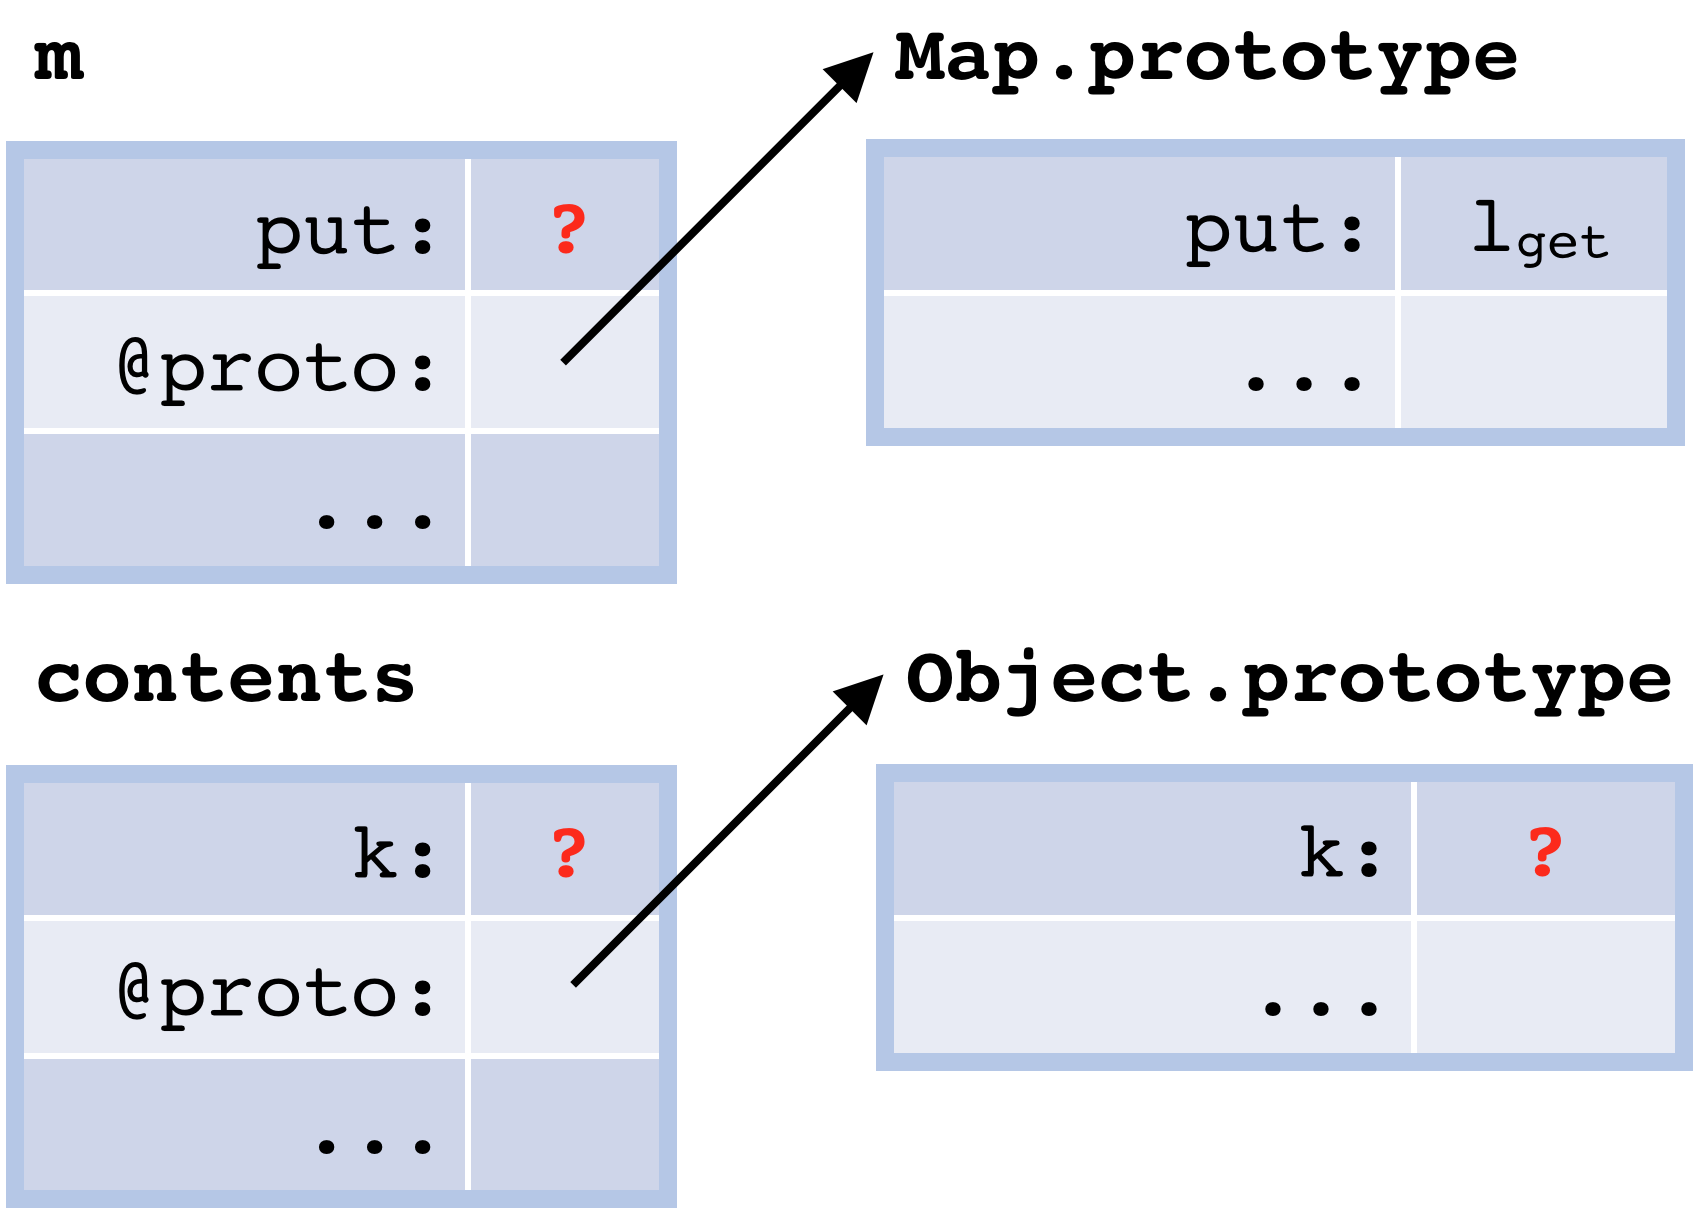
\includegraphics[width=0.21\textwidth]{figures/compositional.png}
\vspace*{-0.58cm}
\caption*{\hspace*{-0.58cm}{\small Figure 2. Compositionality}}
\vspace*{-0.4cm}
\end{wrapfigure}

\setcounter{figure}{2} 
First, if we omitted the part of the \jsinline|Map| predicate highlighted in red, \cosette would complain, when testing the \jsinline|put| function, that it has no information about the property \jsinline|"put"| of the map object~\jsinline|m| and cannot perform the lookup \jsinline|m.put| (Fig.~2, above). This means that the library code is not resilient to frames in which a map object \jsinline|m| has the property \jsinline|put|.
Analogous issues would arise for the \jsinline|"get"| and \jsinline|"validKey"| properties.% which also must be absent from all map objects. 

Second, if we omitted the parts highlighted in blue, upon execution of the line \jsinline|this._contents[k] = v| (Fig.~\ref{fig:2a}, line 12) \cosette would complain that it has no information about the property \jsinline|k| in the prototype chain of the contents object (Fig.~2, below). This is required as the semantics of JavaScript has to look up the value of the property \jsinline|k| of the contents object before performing the actual assignment, to check if the assignment is allowed (i.e.,~ that the property is non-writable). As \jsinline|k| is symbolic, what this means is that the library is not resilient to frames in which there are non-writable properties in \jsinline|Object.prototype|. A similar issue arises for the \jsinline|Map| constructor (Fig.~\ref{fig:2a}, line 1), which requires the property \jsinline|"_contents"| not to be non-writable in the prototype chains of map objects.

%Now, we can give the complete definition of the \jsinline|Map| predicate and the corrected, compositional specification of \jsinline|put(k, v)| when \jsinline|k| is a valid key that is not in the map, with the compositionality-related changes highlighted in red:
%
%\noindent
%\begin{minipage}{0.58\textwidth}
%\begin{Verbatim}[fontsize=\footnotesize,commandchars=\\\{\}]
%  Map (m, mp, kvs) := 
%    JSObjectWithProto(m, mp) * \textcolor{red}{NoProp(m, "get")} * 
%    \textcolor{red}{NoProp(m, "put")} * \textcolor{red}{NoProp(m, "validKey")} * 
%    DataProp(m, "_contents", c) * JSObject(c) *
%    KVPairs(c, kvs) * \textcolor{red}{First(kvs, keys)} * \textcolor{red}{NoProps(c, keys)}
%\end{Verbatim} 
%\end{minipage}
%\begin{minipage}{0.42\textwidth}
%%
%\begin{displaymath} 
%{\scriptsize
%\begin{array}{c}
%\left\{ {\begin{array}{c}
% \text{\texttt{Map(m, mp, kvs) * MapProto(mp) *}} \\
% \text{\texttt{ValidKey(k) * (k $\notin$ First(kvs)) *}} \\
% \text{\textcolor{red}{\texttt{Writable(Object.prototype, k)}}}
%\end{array}} \right\} \\
%%
%\text{\bfseries \texttt{m.put(k, v)}} \\[0.2mm]
%%
%\left\{ {\begin{array}{c}
% \text{\texttt{Map(m, kvs -u- (k, v)) * MapProto(mp) *}} \\
% \text{\textcolor{red}{\texttt{Writable(Object.prototype, k)}}} \\
%\end{array}} \right\}
%\end{array}
%} 
%\end{displaymath}
%\end{minipage}

What this example illustrates is that, in order to be compositional, specifications of programs written in dynamic languages have to explicitly state which parts of the heap must not be present. \cosette is able to detect and report compositionality-related issues, such as those presented above, which are highly likely to remain unnoticed in whole-program analysis, as there we always have complete information about the entire contents of the heap.

%\subsection{Compositional Symbolic Testing}
%
%%\begin{wrapfigure}{R}{0.45\textwidth}
%%\vspace*{-0.5cm}
%%\centering
%%\begin{lstjsex}
%%[ Map(m, mp) * MapProto(mp) * ValidKey(k) ]
%%    m.put(k, v); 
%%    var result = m.get(k);
%%[ Precondition * (result = v) ]
%%\end{lstjsex}
%%\vspace*{-0.4cm}
%%\caption{Revisited test for \jsinline|Map|}
%%\label{test:map:2}
%%\vspace*{-0.35cm}
%%\end{wrapfigure}
%
%A general developer can write concrete and symbolic tests for their code, but cannot be expected to write full functional correctness specifications in separation logic. Using \cosette, they can combine the best of both worlds by describing only the shape of their \polish{heap/memory/data structure} using separation logic and then testing the behaviour of the code using symbolic tests. Using this approach, one can not only find the same bugs as in whole-program symbolic testing, but also detect compositionality issues triggered by the tests. 



%Refer to Figure 2 - the developer knows the heap and can describe it easily. If they forget, . Ideally, this would be automatic.
%
%We illustrate the compositional symbolic execution of \cosette using the \jsinline|get(k)| function of the key-value map example. Below, we revisit the code of \jsinline|get| and describe the heap before and after \jsinline|get(k)| is called with a valid key that is in the map. In order to do this, the developer needs to know the structure of the heap (Figure~\ref{map:example}) and use the built-in predicates.
%
%\smallskip
%\begin{minipage}{0.52\textwidth}
% \begin{lstjs}
%Map.prototype.get = function (k) {
%  var c = this._contents;
%  if this.validKey(k) {
%    return (c.hasOwnProperty(k) ? 
%               c[k] : null)
%  } else throw new Error("Invalid Key");
%}
%\end{lstjs}
%\end{minipage}
%\begin{minipage}{0.47\textwidth}
%$
%{\scriptsize
%\begin{array}{c}
%\left\{{\begin{array}{c}
% \text{\texttt{JSObjectWithProto(this, mp) * MapProto(mp) * }} \\
% \text{\texttt{DataProp(m, "\_contents", c) * JSObject(c) * }} \\
% \text{\texttt{ValidKey(k) * \color{blue}{DataProp(c, k, v)}}}
%\end{array}}\right\} \\
%%
%\text{\bfseries \texttt{get(k)}} \\
%%
%\left\{ {\begin{array}{c}
% \text{\texttt{StartingState * (ret = v)}} 
%\end{array}} \right\}
%\end{array}
%}
%$
%\end{minipage}
%
%\smallskip
%To describe the starting state, we first note that the map object on which \jsinline|get| was called has prototype \jsinline|mp|, representing \jsinline|Map.prototype|.\footnote{Some stuff.} Next, we state that the map object itself has property \jsinline|"_contents"| pointing to a standard JavaScript object \jsinline|c|, that the key \jsinline|k| is valid, and that the object \jsinline|c| has the property \jsinline|k| with value \jsinline|v|. In the final state, we additionally know that the return value of the function should be equal to \jsinline|v|.
%
%
%
%
%
%\vspace*{5cm}
%catch how the spec is not compositional, reveal frame non-resilience shit
%
%It is meant to be run as a method call, the this, it is in the prototype. validKey is also meant to be in the prototype. Refer to figure 2. the this has the contents field, then that is an object, the key k is valid and then it may or may not have the k field.
%
%Now, frame bugs will pop up and you will see how the function is not resilient to the frame.
%
%you can catch these bugs in real-world tests
%
%...and if they want, they can write a more general abstraction of the entire data structure, which may be recursive or not, then ask for it to be unfolded to a given depth and create symbolic tests from that.
%
%
%
%\newpage
%In order for a specification of a program to be compositional, it must be resilient against all the possible frames, that is, all possible contexts in which the program can be run. This is in contrast to whole-program analysis, which considers only one frame at a time. 
%
%we demonstrate how \cosette explicitly exposes the resilience of JavaScript programs to the environment, not  considered by standard symbolic execution tools, but essential for compositional analysis. Therefore, this .
%
%For that, we revisit the \javert specification of key-value maps. This specification involves several predicates, shown below, which use JavaScript-specific abstractions that hide the internals of the language, such as \jsinline|JSObject(c)|, which states that \jsinline|c| is a standard JavaScript object, and \jsinline|DataProp(o, p, v)|, which states that the property \jsinline|p| of \jsinline|o| has value \jsinline|v|.
%
%% \textcolor{red}{(m, "get") -> None * (m, "put") -> None * (m, "validKey") -> None} * 
%
%\begin{Verbatim}[fontsize=\footnotesize,commandchars=\\\{\}]
%    Map (m, kvs) := DataProp(m, "_contents", c) * JSObject(c) * 
%                      KVPairs(c, kvs) * first(kvs, keys) * emptyFields(c, keys)
%\end{Verbatim}
% \begin{Verbatim}[fontsize=\footnotesize,commandchars=\\\{\}]
%KVPairs (o, kvs) := (kvs = \{ \}),
%                    (kvs = (k, v) -u- kvs') * ValidKey(k) * DataProp(o, k, v) * KVPairs(o, kvs')
%\end{Verbatim}
%\begin{Verbatim}[fontsize=\footnotesize,commandchars=\\\{\}]
%    ValidKey (k) := types(k : Str) * \textcolor{red}{(k <> "hasOwnProperty")}
%\end{Verbatim}
%
%
%Refer to Figure 2 - the developer knows the heap and can describe it easily. If they forget, . Ideally, this would be automatic.
%
%The \jsinline|Map| predicate captures the resource corresponding to a map object. 
%Concretely, it first states that the map object has the property \jsinline|_contents|, which points to a  JavaScript object \jsinline|c|.
%Next, using the \jsinline|KVPairs| predicate (explained shortly), it states that \jsinline|c| holds the key-value pairs \jsinline|kvs|. Finally, it obtains the set of keys \jsinline|keys| from the set of key-value pairs using the first projection predicate \jsinline|first|, and then, via the \jsinline|emptyFields| assertion, states that all other properties are absent from \jsinline|c|.
%
%The \jsinline|KVPairs(o, kvs)| predicate talks about key-value pairs of an object \jsinline|o|. 
%It is defined recursively on the structure of \jsinline|kvs| and it has two definitions, separated by a comma. 
%We have that \jsinline|kvs| is either empty or that it contains at least one key-value pair \jsinline|(k, v)|,\footnote{We write $\mathtt{-u-}$ for set union and omit the brackets around singleton sets.} 
%in which case we state that the key \jsinline|k| must be valid, that object \jsinline|o| has  property \jsinline|k| with value \jsinline|v|, and proceed recursively.
%The uniqueness of keys is guaranteed by the \jsinline|DataProp| predicate of \jsinline|KVPairs| and the separating conjunction.
%
%\begin{wrapfigure}{R}{0.3\textwidth}
%\vspace*{-0.45cm}
%\centering
%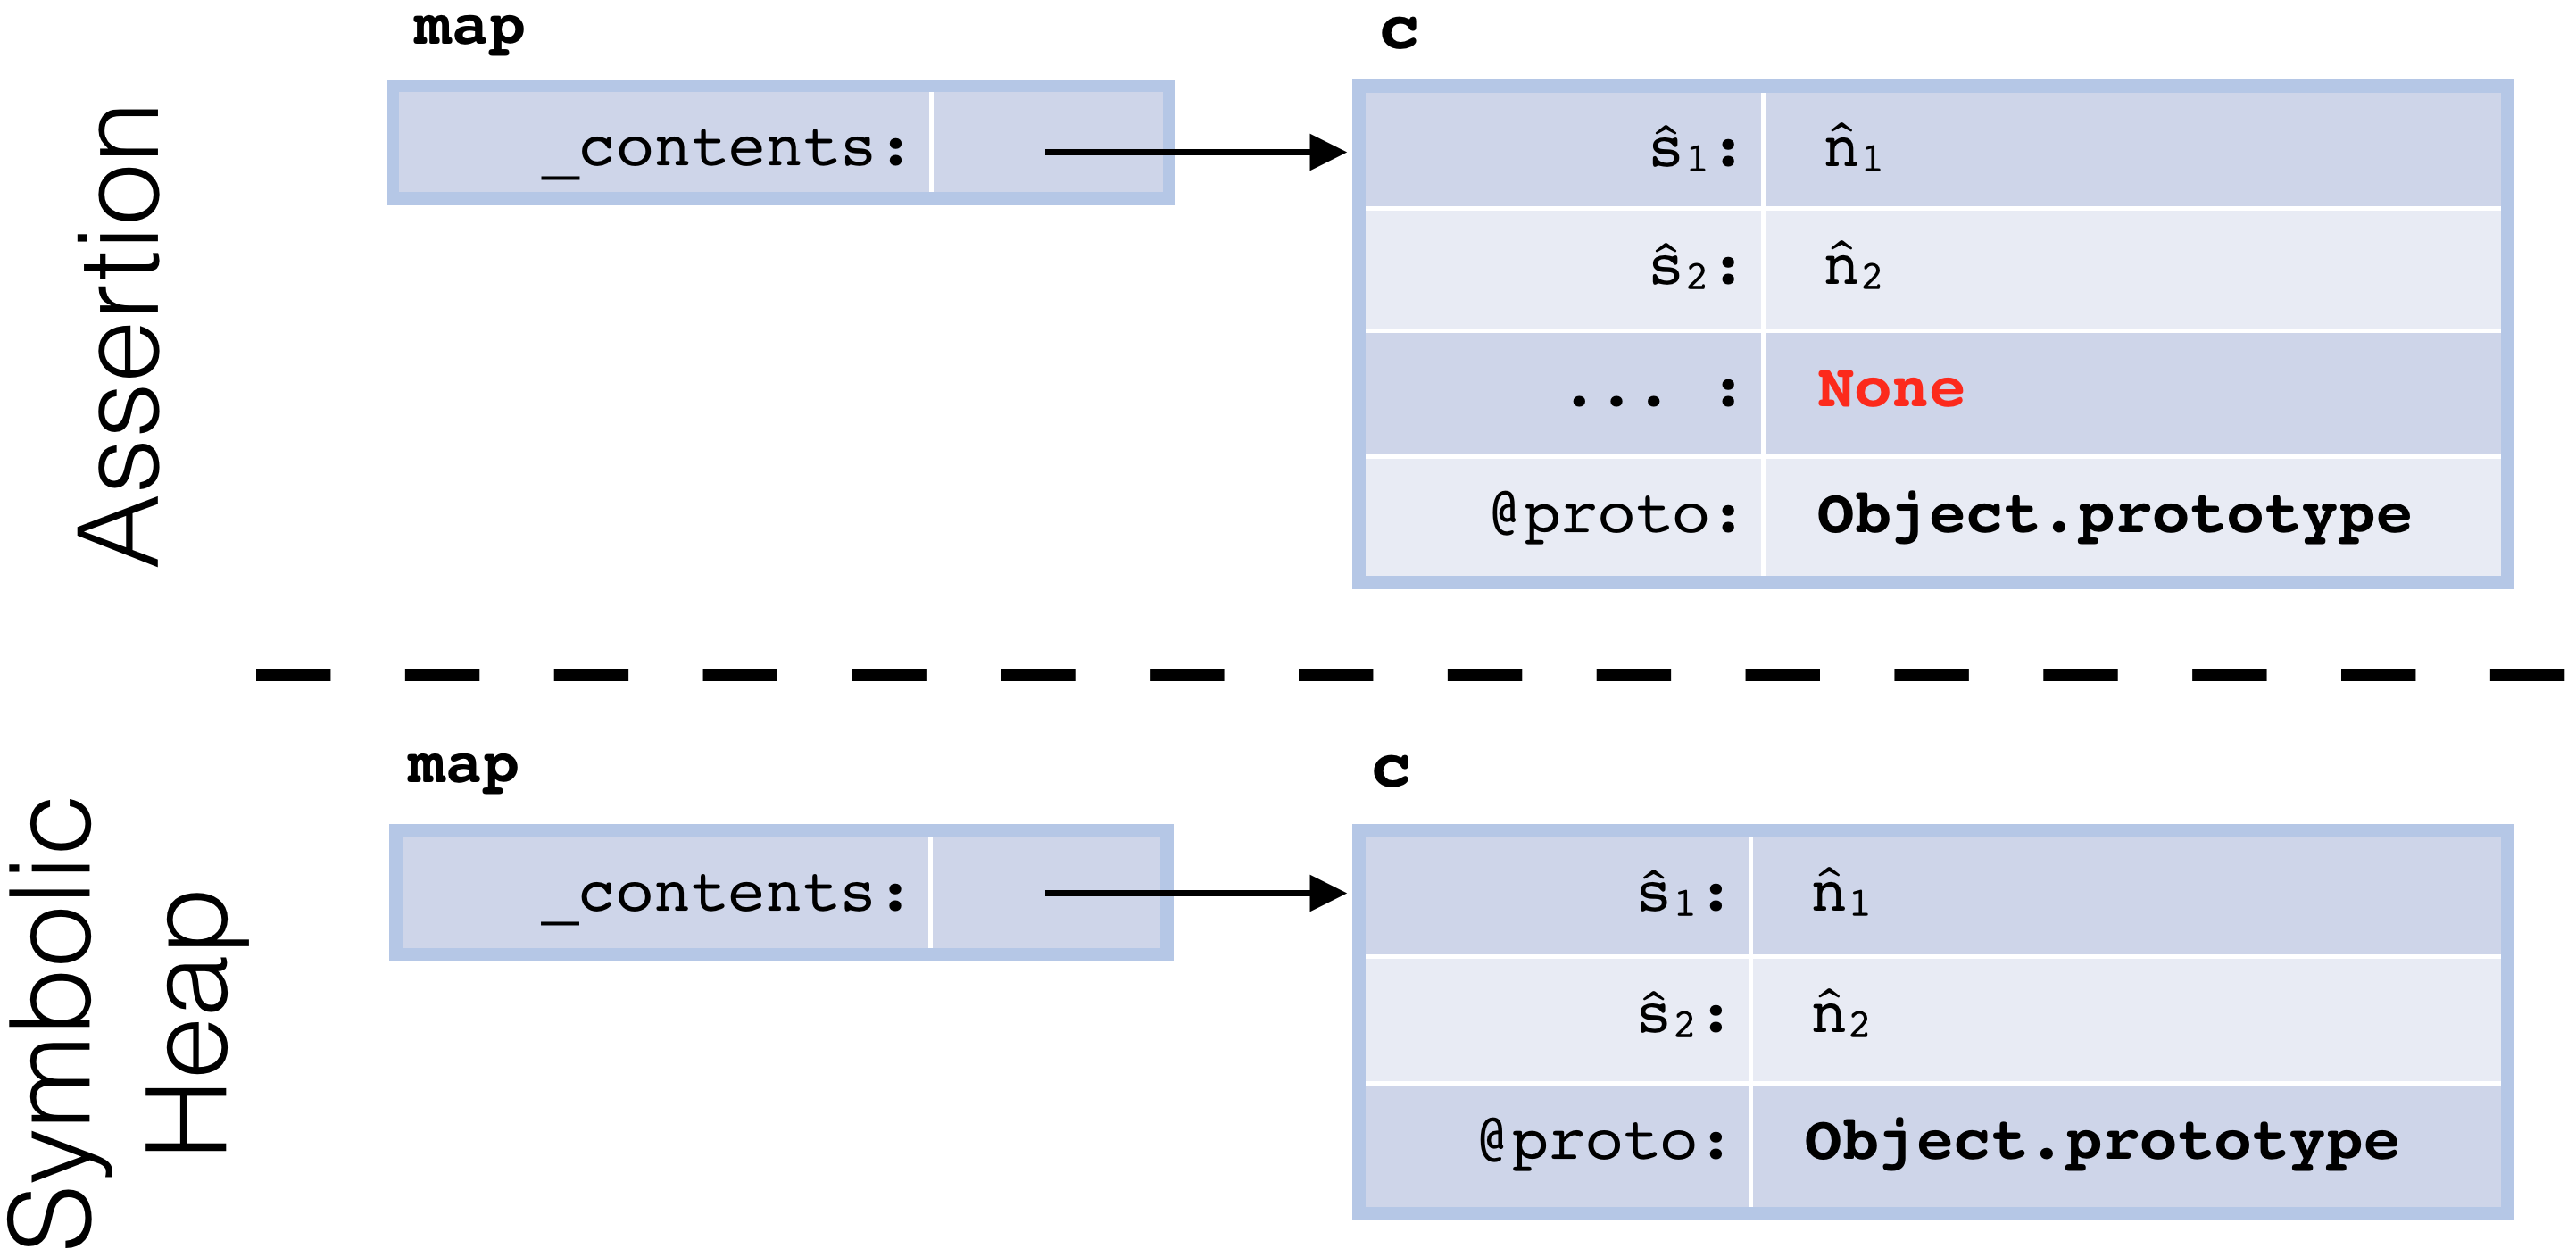
\includegraphics[width=0.29\textwidth]{figures/symbvsass.png}
%\vspace*{-0.3cm}
%\caption{Unfolded assertion {\scriptsize$\mathtt{Map(map, \{ (\hat{s}_1, \hat{n}_1), (\hat{s}_2, \hat{n}_2) \} )}$}}\label{fig:symb:state:versus:assertion}
%\label{fig:unfolded}
%\vspace*{-0.4cm}
%\end{wrapfigure}
%
%The \jsinline|ValidKey(k)| predicate captures the validity of a given key and holds \emph{iff} the corresponding JavaScript function \jsinline|validKey(k)| returns \jsinline|true|.
%In the definition of \jsinline|ValidKey|, we highlight in red a potential bug in the specification, already seen in the symbolic testing example.
%% source of errors on which we will focus shortly.
%
%To give a better intuition of how the \jsinline|Map| predicate works, we show the full unfolding of {\small$\mathtt{Map(map, \{ (k_1, v_1), (k_2, v_2) \} )}$} in Figure \ref{fig:symb:state:versus:assertion}. 
%
%\noindent
%\begin{minipage}{0.475\textwidth}
%\begin{displaymath} 
%{\scriptsize
%\hspace*{-0.2cm}
%\begin{array}{c}
%\left\{ {\begin{array}{c}
% \text{\texttt{Map(this, kvs -u- (k, v)) * ObjProtoF() *}} \\
% \text{\texttt{(this, "@proto") -> mp * MapProto(mp) * ...}}
%\end{array}} \right\} \\
%%
%\text{\bfseries \texttt{get(k)}} \\[0.2mm]
%%
%\left\{ {\begin{array}{c}
% \text{\texttt{Precondition * (ret = v)}} 
%\end{array}} \right\}
%\end{array}
%} 
%\end{displaymath}
%\end{minipage}
%\quad
%\begin{minipage}{0.48\textwidth}
%%
%\begin{displaymath} 
%{\scriptsize
%\begin{array}{c}
%\left\{ {\begin{array}{c}
% \text{\texttt{Map(this, kvs -u- (k, v')) * ObjProtoF() *}} \\
% \text{\texttt{(this, "@proto") -> mp * MapProto(mp) * ...}}
%\end{array}} \right\} \\
%%
%\text{\bfseries \texttt{put(k, v)}} \\[0.2mm]
%%
%\left\{ {\begin{array}{c}
% \text{\texttt{Map(this, kvs -u- (k, v)) * ObjProtoF() *}} \\
% \text{\texttt{(this, "@proto") -> mp * MapProto(mp) * ...}}
%\end{array}} \right\}
%\end{array}
%} 
%\end{displaymath}
%\end{minipage}
%
%\vspace{5pt}
%The predicate \jsinline|ObjProtoF()| describes the \jsinline|Object.prototype| object. It is needed because \jsinline|get| uses the \jsinline|hasOwnProperty| function, defined in \jsinline|Object.prototype|. 
%The predicate \jsinline|MapProto| specifies the resource of a valid map prototype: in particular, it defines the \jsinline|put|, \jsinline|get|, and \jsinline|validKey| methods.
%
%Given a JavaScript function, its separation logic specification, and the depth to which the unfold recursive predicates (non-recursive predicates are unfolded automatically), \cosette generates symbolic tests to verify that the function conforms to the specification up to that given depth.
%Now, if we forgot to state the part of the \jsinline|ValidKey(k)| predicate highlighted in red, that is, if we did not state that \jsinline|k <> "hasOwnProperty"|, the symbolic test generated for the specification of \jsinline|get| would fail for depth $\geq 1$, with the counter-model \jsinline|k = "hasOwnProperty"|, triggering the same bug previously described in the context of symbolic testing.

%\subsection{Catching \polish{procedure-local} bugs}
%
%The bug associated with the shadowing of the \jsinline|hasOwnProperty| property of \jsinline|Object.prototype| illustrates how a JavaScript library can be broken by only using its own functions. However, as JavaScript does not observe the frame property, there exists an additional class of bugs that can be triggered by the environment in which the library is run. These bugs expose how the library is not resilient against the possible frames and signal which properties of which objects must not be present in order for the library to behave correctly.
%
%To illustrate such bugs, recall the symbolic test from \S\ref{subsec:st}. This symbolic test creates an empty map on which it checks whether or not the behaviour of \jsinline|put| is correct. After catching the \jsinline|hasOwnProperty| bug, one might want to construct a more general test, starting from an arbitrary map. For this, one would need to use the \jsinline|Map| predicate from \S\ref{subsec:sdbf}:
%
%\begin{Verbatim}[fontsize=\footnotesize,commandchars=\\\{\}]
%         Map (m, kvs) := DataProp(m, "_contents", c) * JSObject(c) * 
%                           KVPairs(c, kvs) * first(kvs, keys) * emptyFields(c, keys)
%\end{Verbatim}
%
%\noindent as part of the initial state in which to run the symbolic test. Then, however, on execution of the test, when we reach the \jsinline|m.put(k, v)| command, we will get an error. The symbolic execution will not be able to determine if the property \jsinline|put|, which is supposed to be found in \jsinline|Map.prototype|, exists in the object~\jsinline|m| or not. This means that an environment can break the map library by putting into a map object the properties that are meant to be found in its prototype, and also that the specification of maps needs to be strengthened to forbid this explicitly:
%\begin{Verbatim}[fontsize=\footnotesize,commandchars=\\\{\}]
%   Map (m, kvs) := DataProp(m, "_contents", c) * JSObject(c) * 
%                     \textcolor{red}{((m, "get) -> none)} * \textcolor{red}{((m, "put") -> none)} * \textcolor{red}{((m, "validKey") -> none)} *
%                       KVPairs(c, kvs) * first(kvs, keys) * emptyFields(c, keys).
%\end{Verbatim}
%
%Bugs such as this will very rarely be caught by whole-program analyses, because there the entire state of the program is known and the test needs to be especially crafted with these bugs in mind. The reason that \cosette can catch them easily is because it is compositional and can run in partially described states.


\section{Symbolic Execution for \jsil}\label{sec:jsil:symb:exec}
%!TEX root = ../main.tex

We present our new methodology for designing compositional program analyses for dynamic languages and apply it to obtain a compositional symbolic execution engine for \jsil, an intermediate representation for JavaScript analysis~\cite{javert}.
%
%Much like JavaScript, \jsil does not exhibit the frame property~\cite{reynolds:lics:2002}, raising the issue of how to guarantee that the results of the analysis still hold when extending the initial state of the analysed program with a given arbitrary frame.
%
%The methodology has three steps: \dtag{1} designing an instrumented semantics of the language that exhibits the frame property, \dtag{2} designing the program  analysis on the instrumented semantics, and \dtag{3} linking the program analysis to the concrete semantics by describing the frames that can be safely added to the initial state.   
%
%The key innovation is to have the instrumented semantics as a proper interim stage in the design of the analysis, obtaining 
%more modular reasoning and substantially simpler proofs.
%
%For our symbolic analysis, 
We define a new, abstract semantics for \jsil,\footnote{We refer to the semantics as \emph{abstract} since it 
is parametric on a \jsil state signature. We are not doing abstract interpretation.} in the spirit %style % I think style is too strong because the citation is really abstract interpretation - it will be very confusing
 of~\cite{vanhorn:icfp:2010}, which we instantiate to obtain the concrete, instrumented, and symbolic semantics. 
This abstract semantics is the bedrock for both the formal development \emph{and} the implementation of the analysis. This approach has several benefits: it streamlines the formalism, avoiding redundancy; it makes the choices in the design of the instrumented and symbolic semantics explicit; and it leads to modular implementations, avoiding code duplication.
%
Full definitions and proofs are given in the~Appendix.

%In \S\ref{subsec:jsil:analysis:formalism}, we define an abstract semantics for 
%\jsil, which we then instantiate to obtain its concrete and symbolic semantics.
%In \S\ref{sex:formal:guarantees}, we present the formal guarantees of 
%our symbolic analysis, including: \dtag{i} a soundness result for the \jsil symbolic 
%execution, \dtag{ii} a guarantee of absence of false positives for bug-finding, \pmaxinline{Do we know what bug-finding is here?}
%\dtag{iii} a justification result for the lifting of analyses on compiled \jsil code back to JavaScript;
%and \dtag{iv} \polish{a verification result that precisely states the conditions 
%under which symbolic execution gives us verification guarantees.}
%Finally, in \S\ref{subsec:jsil:analysis:implementation}, we give a brief overview
%of our implementation. %in \rosette~\cite{Rosette1,Rosette2} NO NO NO! Burn the witch!

\vspace*{-0.2cm}
\subsection{\jsil Syntax and Abstract Semantics}\label{subsec:jsil:analysis:formalism}

\vspace*{-0.1cm}
\myparagraph{Syntax} \jsil is a simple goto language featuring top-level procedures and commands that operate on object heaps. It was purposefully designed to natively support the main dynamic features of JavaScript: extensible objects; dynamic property access; and dynamic procedure calls. The syntax of \jsil is shown below. 

\vspace{5pt}
\begin{display}{Syntax of the \jsil Language}{
\begin{tabular}{l}
	% $\jnumber \in \numbers$ \jspc  $\jbool \in \bools$ \jspc $\jstring \in \strings$  \jspc 
	% $\loc \in \locs$ \jspc $\jvar \in \jvars$ \jspc $\jtype \in \jtypes$ \\[0.1cm]
	 %
$\val \in \vals$ \defeq\ $\jnumber \! \mid \! \jbool \! \mid \! \jstring \! \mid \! {\small \jundefined} \! \mid \! {\small \jnull} \! \mid \! {\small \jempty} \! \mid \! \loc \! \mid \! \jtype \! \mid \!  \pid \! 
         \mid \! \jsillist{\val_i\!\!\mid_{i=0}^n} \! \mid \! \jsilset{\val_i \!\!\mid_{i=0}^n}$
   \\[0.1cm]
 %
  $\jsilexpr \in \exprs$ \defeq\ $\val \mid \jvar \mid \svar \mid \ominus\ \jsilexpr \mid \jsilexpr \binop{} \jsilexpr$
 \\[0.1cm]
%
$\bcmd \in \bcmds$ \defeq\ $\jsilskip \mid \jvar := \jsilexpr  \mid \jvar := \jsilnew() \mid \jvar := [\jsilexpr, \jsilexpr] \mid [\jsilexpr, \jsilexpr] := \jsilexpr $ \\
%
\hspace{0.02cm} $\mid \jsildelete(\jsilexpr, \jsilexpr) \mid \jvar := \hasfield(\jsilexpr, \jsilexpr) \mid \jvar := \getfields(\jsilexpr)$ \\[0.1cm]
% Commands
$\jcmd \in \cmds$ \defeq \ $ \bcmd \mid \goto \ i \mid  \ifgoto{\jsilexpr}{i}{j} \mid \jsilcall{\jvar}{\jsilexpr}{\jsilexpr_i\!\!\mid_{i=0}^n}{j}$ \\
\hspace{0.02cm} $ \mid \assume(\jsilexpr) \mid \jassert(\jsilexpr)$ \\[0.1cm]
%
$\proc \in \procs$ \defeq \ $\procedure{\pid}{\jvec{\jvar}}{\jvec{\jcmd}}$
\hspace{0.6cm}
$i, j \in \indexes$ $\semeq \mathbb{N} \cup \{ \retlab, \errlab \}$
 \end{tabular}}
\end{display}

\vspace{2pt}
\noindent \jsil \emph{values}, $\val \in \vals$, include numbers, booleans, strings, the special values $\jundefined$, $\jnull$, and $\jempty$, object locations~$\loc$, types~$\jtype$, procedure identifiers $\pid$, and lists and sets of values.
\jsil~\emph{expressions}, $\jsilexpr \in \exprs$, include \jsil values, \jsil program variables $\jvar$, various unary and binary operators, and symbolic variables $\svar$, introduced in this paper. Symbolic variables range over symbolic strings, numbers, booleans, and locations, denoted respectively by $\sstring$, $\snumber$, $\sbool$, and~$\sloc$.

%

\jsil \emph{basic commands} enable the manipulation of extensible objects and do not affect control flow. 
They include $\jsilskip$, variable assignment, object creation, property access, property assignment, property deletion, membership check, and property collection.
%, and a new command for symbolic variable creation. 
%
\jsil \emph{commands} include \jsil basic commands and control flow commands: conditional and unconditional gotos, dynamic procedure calls, and two new commands for symbolic reasoning, $\assume$ and $\jassert$.  %\footnote{\jsil also has a $\phi$-node assignment (cf.~\cite{javert}), supporting Static-Single-Assignment (SSA) \cite{SSA}. To avoid clutter, we omit it as it does not impact the reasoning.} 
The goto commands are intuitive: $\goto \ i$ jumps to the $i$-th command of the active procedure, and $\ifgoto{\jsilexpr}{i}{j}$ jumps to the $i$-th command if $\jsilexpr$ evaluates to $\jtrue$, and to the $j$-th otherwise. 
The dynamic procedure call $\jsilcall{\jvar}{\jsilexpr}{\jvec{\jsilexpr}}{j}$ evaluates  $\jsilexpr$ and $\jvec{\jsilexpr}$ to obtain the procedure identifier and arguments, respectively, executes the appropriate procedure with these arguments, and, in the end, assigns its return value to $\jvar$.
If the procedure raises an error, control is transferred to the $j$-th command; otherwise, it follows to the next command. 
%

A \jsil procedure is of the form $\procedure{\pid}{\jvec{\jvar}}{\jvec{\jcmd}}$, where $\pid$ is its identifier, $\jvec{\jvar}$ are its formal parameters, and its body ${\jvec{\jcmd}}$  is a sequence of \jsil commands. 
%\polish{When calling a procedure, any missing parameters are implicitly set to $\jundefined$.}
Procedures return via two dedicated indexes, $\retlab$ and $\errlab$, using two dedicated variables, $\retvar$ and $\errvar$. If a procedure reaches the $\retlab$ index, it returns normally with the return value denoted by $\retvar$; if it reaches $\errlab$, it returns an error, with the error value denoted by $\errvar$.
%
A \jsil program $\prog \in \progs$ is a set of top-level procedures, and its entry point is always the special procedure $\jsilmain$\hspace{-2pt}.


%
%\pmax{more modular, factor out. three for symbolic analysis}
\myparagraph{Abstract semantics} We design the abstract semantics to make the analysis, the proofs, and the implementations as modular as possible. At its core are the GetCell and GetDomain functions, which precisely pinpoint the way in which \jsil interacts with the heap, factoring out the common behaviour of \jsil basic commands. It also provides standard constructs for reasoning about symbolic values, whose concrete and instrumented semantics are trivial.

The abstract semantics is parametric on abstract states $\absstate \in \absstates$ and abstract values $\absval, \absprop, \absloc \in \absvals$. 
%For clarity, we use $\absprop$ and $\absloc$ to refer to abstract values denoting properties and locations, respectively.
%
Abstract states are assumed to have a store $\absstore: \jvars \partialmap \absvals$, mapping program variables $\jvar \in \jvars$ to abstract values. Stores are accessible via a store selector, $\absstate.\stosel$.
We use the special symbol $\none$ (read: none) to denote the absence of a property in an object, write $\setext{\absvals}{\none}$ for the set $\absvals \cup \{ \none \}$ and range over it using~$\iabsval$.
Abstract states expose the following functions and relations: 
\begin{description}
\setlength{\itemsep}{0.2em}
  \item[\jsil Expression Evaluation,] $\evalexpr{}(\absstore, \jsilexpr)$, which evaluates to the value of the \jsil expression $\jsilexpr$ under store $\absstore$. 

  %\item[Store Selector,] $\stosel : \absstates \rightarrow (\jvars \partialmap \absvals)$. The expression $\stosel(\absstate)$ evaluates to the store associated with a given  state $\absstate$. For clarity, we write $\absstate.\stosel$ instead of $\stosel(\absstate)$. 

  \item[Store Update,] $\stupdt{}(\absstate, \jvar, \absval)$, which denotes the state obtained from $\absstate$ 
             by updating the value of $\jvar$  to $\absval$ in $\absstate.\stosel$. 

  \item[Heap Allocation,] $\absalloc{}(\absstate)$, which evaluates to a pair consisting of a value denoting a fresh location and the new state that keeps track of that allocation. %
%             

   \item[Heap Update,] $\hpupdt{}(\absstate, \absloc, \absprop, \iabsval)$, denoting the state obtained from $\absstate$ by updating the value of property $\absprop$ of the object at location $\absloc$ to~$\iabsval$ or creating that property, in the
             case it does not exist.

  \item[GetCell,] $\absgetcellrule{}{\absstate, \jsilexpr_1, \jsilexpr_2}{\absstate', (\absloc, \absprop, \iabsval)}$, which retrieves the value associated with a given property of a given object. Formally, if $\absgetcellrule{}{\absstate, \jsilexpr_1, \jsilexpr_2}{\absstate', (\absloc, \absprop, \iabsval)}$ holds, 
          then: $\absloc$ denotes the location resulting from the evaluation of $\jsilexpr_1$, 
          $\absprop$~denotes the property name resulting from the evaluation of $\jsilexpr_2$, 
          $\iabsval$~denotes the value of the property $\absprop$ of the object at location $\absloc$, 
          and $\absstate'$ denotes a potential re-arrangement of $\absstate$ after property inspection (discussed in \S\ref{subsec:instrumented}). 
          %Observe the wide use of $\getcell$ in the abstract semantics of the basic commands (Figure~\ref{abs:sem:bcmds:fig}).
          %Also, $\getcell$ is non-deterministic and is, therefore, a relation.
            

               
             
  \item[GetDomain,] $\absgetdomainfun{}(\absstate, \jsilexpr)$, which denotes the 
           set of property names associated with the object at location resulting from the evaluation of $\jsilexpr$ 
           in $\absstate$. It is used in the \textsc{Property Collection} rule.
   
   %\item[Symbolic Value Creation,] $\absmakesymbolicrule{}{\jtype}$, which evaluates to a fresh  value of type $\jtype$.
   
   \item[Assumption,] $\absassume{}(\absstate, \jsilexpr)$, denoting the state obtained from $\absstate$ by stating that $\jsilexpr$ is assumed to evaluate to $\jtrue$. 
  
   \item[SAT Check,] $\abssat{}(\absstate, \jsilexpr)$, which evaluates to $\jtrue$ if the \jsil expression $\jsilexpr$ is satisfiable in the state~$\absstate$, and to $\jfalse$ otherwise.
             
\end{description}

\begin{figure}[t!]
{\scriptsize
\begin{mathpar}
  \inferrule[\textsc{Skip}]{}
	{ \absbsemrule{\absstate, \jsilskip}{\absstate}{}}  	
\qquad 
\inferrule[\textsc{Property Collection}]
  {
           \absval = \absgetdomainfun{}(\absstate, \jsilexpr)  
           \quad
           \absstate' =  \stupdt{}(\absstate, \jvar, \absval)
  }{\absbsemrule{\absstate, \jvar := \getfields(\jsilexpr)}{\absstate'}{}} 
\qquad 
\inferrule[\textsc{Assignment}]
  {
        \absstore = \absstate.\stosel
        \quad 
        \absval = \evalexpr{}(\absstore, \jsilexpr)
  }{\absbsemrule{\absstate, \jvar := \jsilexpr}{\stupdt{}(\absstate, \jvar, \absval)}{}} 
\\
\inferrule[\textsc{Object Creation}]
  { 
     (\loc, \absstate') = \absalloc{}(\absstate)   
      \qquad \absgetcellrule{}{\absstate', \loc, \protop}{\absstate'', -} \\\\ \absstate''' = \hpupdt{}(\absstate'', \loc, \protop, \jnull)
       }{\absbsemrule{\absstate, \jvar := \jsilnew()}{\stupdt{}(\absstate''', \jvar, \loc)}{}}
\qquad  
\inferrule[\textsc{Property Access}]
  { 
  	\absgetcellrule{}{\absstate, \jsilexpr_1, \jsilexpr_2}{\absstate', (-, -, \absval)}
  }{ \absbsemrule{\absstate, \jvar := [\jsilexpr_1, \jsilexpr_2]}{\stupdt{}(\absstate', \jvar, \absval)}{}}
%
\\
\inferrule[\textsc{Property Assignment}]
  {    
      \absgetcellrule{}{\absstate, \jsilexpr_1, \jsilexpr_2}{\absstate', (\absloc, \absprop, -)} 
      \\\\ \absstore = \absstate.\stosel \quad \absval = \evalexpr{}(\absstore, \jsilexpr_3)
  }{\absbsemrule{\absstate, [\jsilexpr_1, \jsilexpr_2] := \jsilexpr_3}{\hpupdt{}(\absstate', \absloc, \absprop, \absval)}{}} 
\qquad 
 \inferrule[\textsc{Property Deletion}]
  { 
        \absgetcellrule{}{\absstate, \jsilexpr_1, \jsilexpr_2}{\absstate', (\absloc, \absprop, \absval)}
  }{\absbsemrule{\absstate, \jsildelete(\jsilexpr_1, \jsilexpr_2)}{\hpupdt{}(\absstate', \absloc, \absprop, \none)}{}}
\\
\inferrule[\textsc{Member Check - True}]
  { 
     \absgetcellrule{}{\absstate, \jsilexpr_1, \jsilexpr_2}{\absstate', (-, -, \absval)}
     \\\\
    \absstate'' = \stupdt{}(\absstate', \jvar, \jtrue)
  }{\absbsemrule{\absstate, \jvar := \hasfield(\jsilexpr_1, \jsilexpr_2)}{\absstate''}{}}
 \qquad  
 \inferrule[\textsc{Member Check - False}]
  { 
     \absgetcellrule{}{\absstate, \jsilexpr_1, \jsilexpr_2}{\absstate', (-, -, \none)} 
     \\\\
    \absstate'' = \stupdt{}(\absstate', \jvar, \jfalse)
  }{\absbsemrule{\absstate, \jvar := \hasfield(\jsilexpr_1, \jsilexpr_2)}{\absstate''}{}}
%\inferrule[\textsc{Member Check - False}]
%  { 
%     \absgetcellrule{}{\absstate, \jsilexpr_1, \jsilexpr_2}{\absstate', (-, -, \none)} 
%     \\\\
%     \absstate'' =  \stupdt{}(\absstate', \jvar, \jfalse)
%  }{\absbsemrule{\absstate, \jvar := \hasfield(\jsilexpr_1, \jsilexpr_2)}{\absstate''}{}} \\
%  \inferrule[\textsc{Make Symbolic}]
%  { 
%     \absval = \absmakesymbolicrule{}{\absstate, \jtype}
%  }{\absbsemrule{\absstate, \jvar := \makesymbolic(\jtype)}{\stupdt{}(\absstate, \jvar, \absval)}{}}
\end{mathpar}}
\vspace*{-0.5cm}
 \captionsetup{format=nastyCaption}
\caption*{{\small Figure 3. Abstract semantics, basic commands: $\absbsemrule{\absstate, \bcmd}{\absstate'}{}$}}\label{abs:sem:bcmds:fig}
\vspace*{-0.4cm}
\end{figure}

%Assumption and the satisfiability check have trivial concrete semantic.

\noindent Transitions for basic commands have the form 
{\small $\absbsemrule{\absstate, \bcmd}{\absstate'}{}$}, meaning that the execution of the basic command 
$\bcmd$ in the state $\absstate$ results in the state $\absstate'$ (Fig.~3). 
%
To describe transitions of commands, we introduce \emph{execution modes}, $\mode$, and 
\emph{call stacks},~$\abscs$.  \jsil has two execution modes: 
$\top$, meaning the execution can proceed; and~$\bot$, meaning that the execution must stop due to an \emph{assert failure}. Call stacks are lists of tuples of the form $(\pid, \absstore, \jvar, i, j)$, where: 
$\pid$~is the identifier of the executing procedure;
$\absstore$~is the store of the procedure that called~$\pid$; 
$\jvar$~is the variable that will hold the return value of~$\pid$; %in~$\absstore$; 
and $i$ ($j$) is the index to which the control jumps when $\pid$ returns normally (with an error). 
%$i$ is the command index to which the control jumps when $\pid$ returns normally; 
%and $j$ is the command index to which the control jumps when $\pid$  returns an error. 
The \emph{initial call stack}, $\csmain$, is defined as {\small $[ (\jsilmain, \storeemp, \jsilout, 0, 0) ]$}, where ${\small\jsilout}$ holds the output of the entire program.  
Transitions for  commands have the form  {\small $\prog: \abssemrule{\absstate, \abscs, i}{\absstate', \abscs', j}{\mode}{\mode'}{}$}, 
meaning that, given a program~$\prog$, state~$\absstate$ and execution mode~$\mode$, the evaluation of the $i$-th command of the first procedure of %the call stack~
$\abscs$ generates 
the state~$\absstate'$, call stack $\abscs'$,  and the next command to be evaluated is the $j$-th command of the first procedure 
of~$\abscs'$, in execution mode~$\mode'$ (Fig.~4). 
For clarity, we keep the program implicit and write {\small $\ccmd{\abscs, i}$} to denote the $i$-th command of the first procedure of $\abscs$.

% We write $\ccmd{i}$ when $\prog$ and $\abscs$ are implicit.
%\vspace{-3pt}
\myparagraph{Notation} In the following, we denote a function with an empty domain by $\hemp$, and for a function $f : A \partialmap B$, we denote its domain extension/update by $f[a \mapsto b]$ %, denoting the heap $\heap$ extended with $\heap(\loc,\jstring) = \val$;
and the union of two functions with disjoint compatible domains by $f_1 \dunion f_2$. 

\begin{table*}[t!]
\centering 
{\scriptsize \begin{tabular}{@{}c@{}ccc@{}c@{}}\toprule
\multicolumn{3}{c}{{\it Concrete Execution: successful (left); failing (right)}} & &  \emph{Instrumented Execution}  \\
%\cmidrule{1-3} \cmidrule{5-5}
%\emph{Successful}  &  & \emph{Failing}  &   &       \\
\cmidrule{1-3} \cmidrule{5-5}
{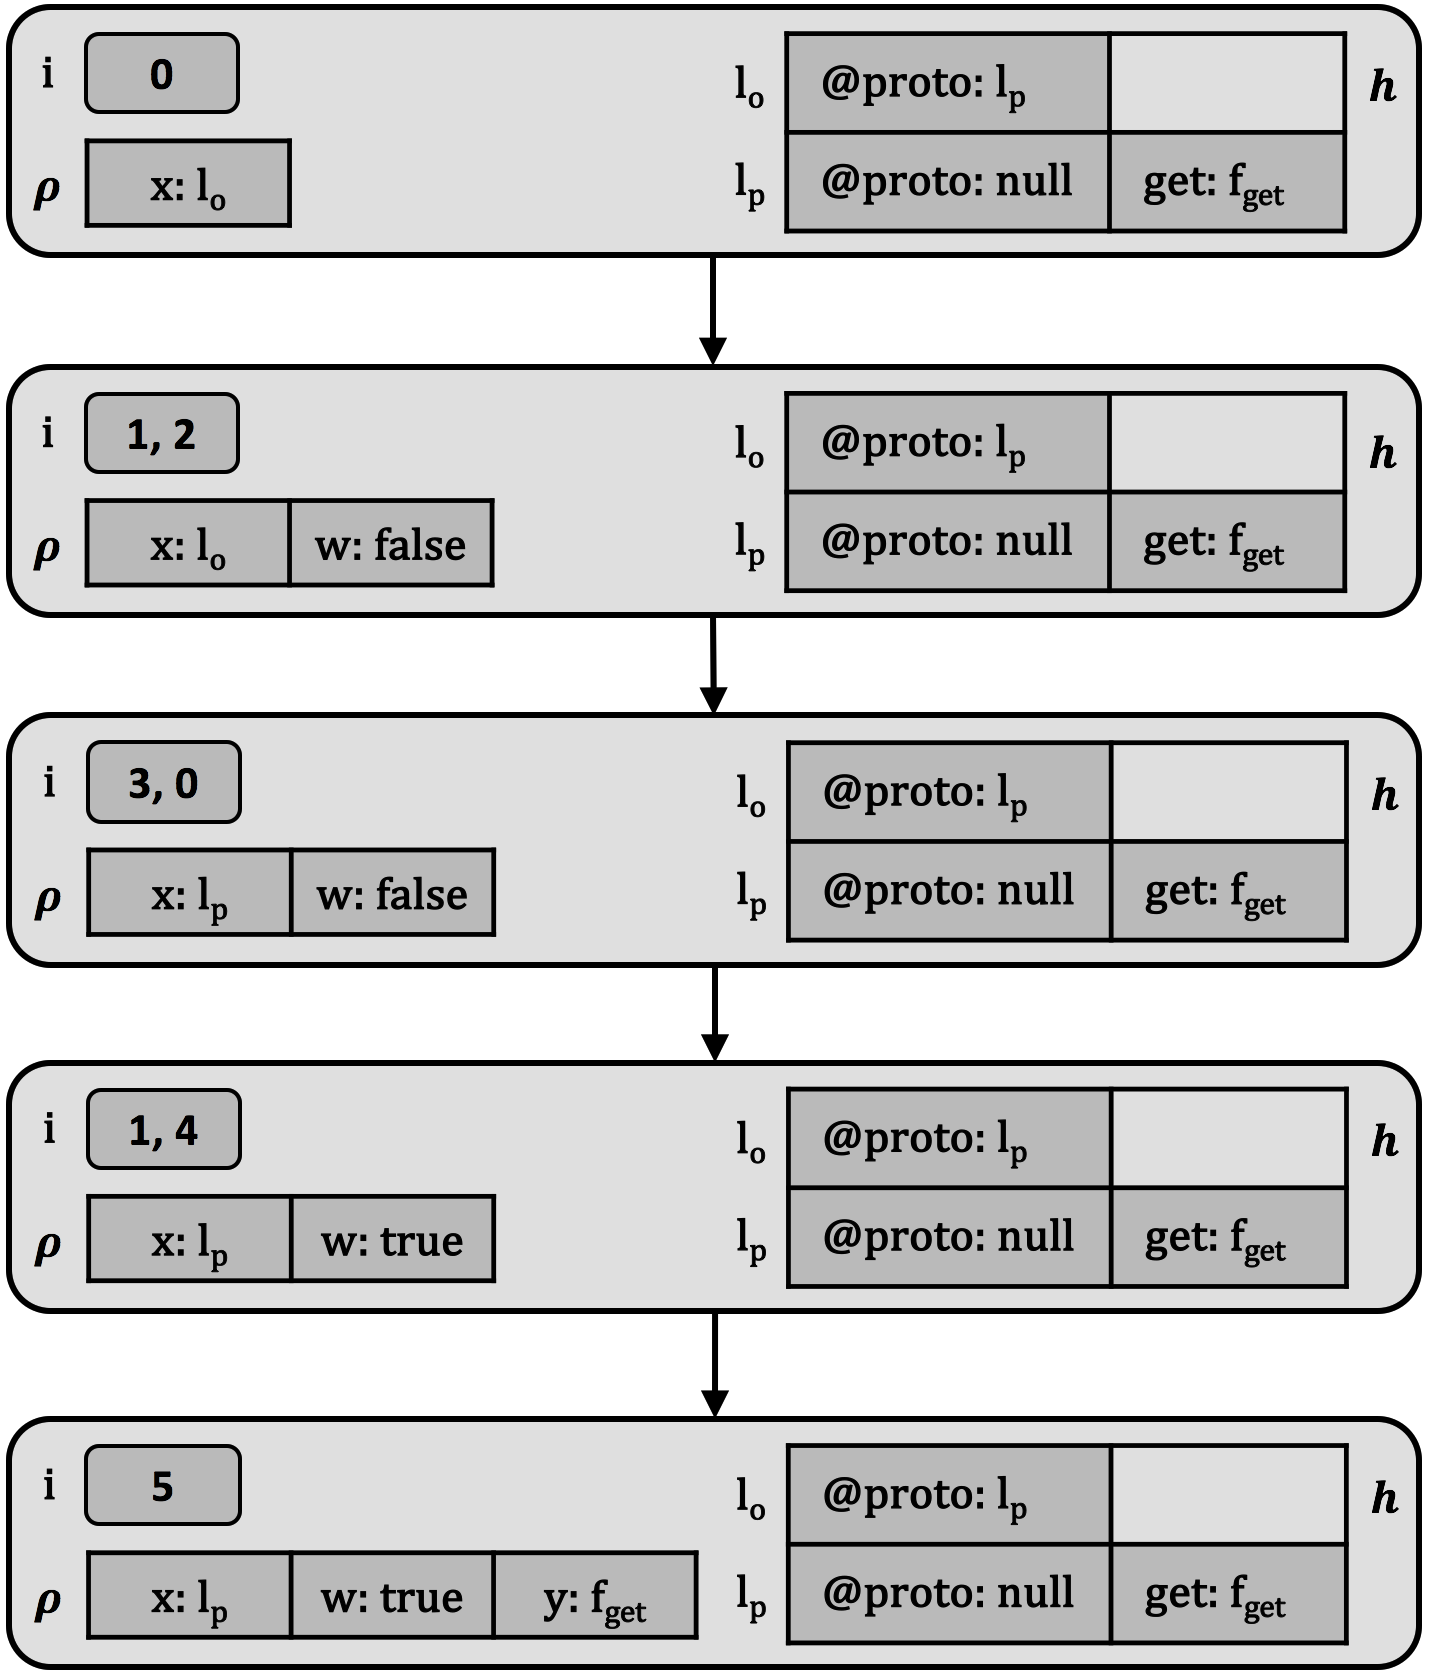
\includegraphics[width=0.305\textwidth,valign=T]{figures/conc_exec.png}} & & 
{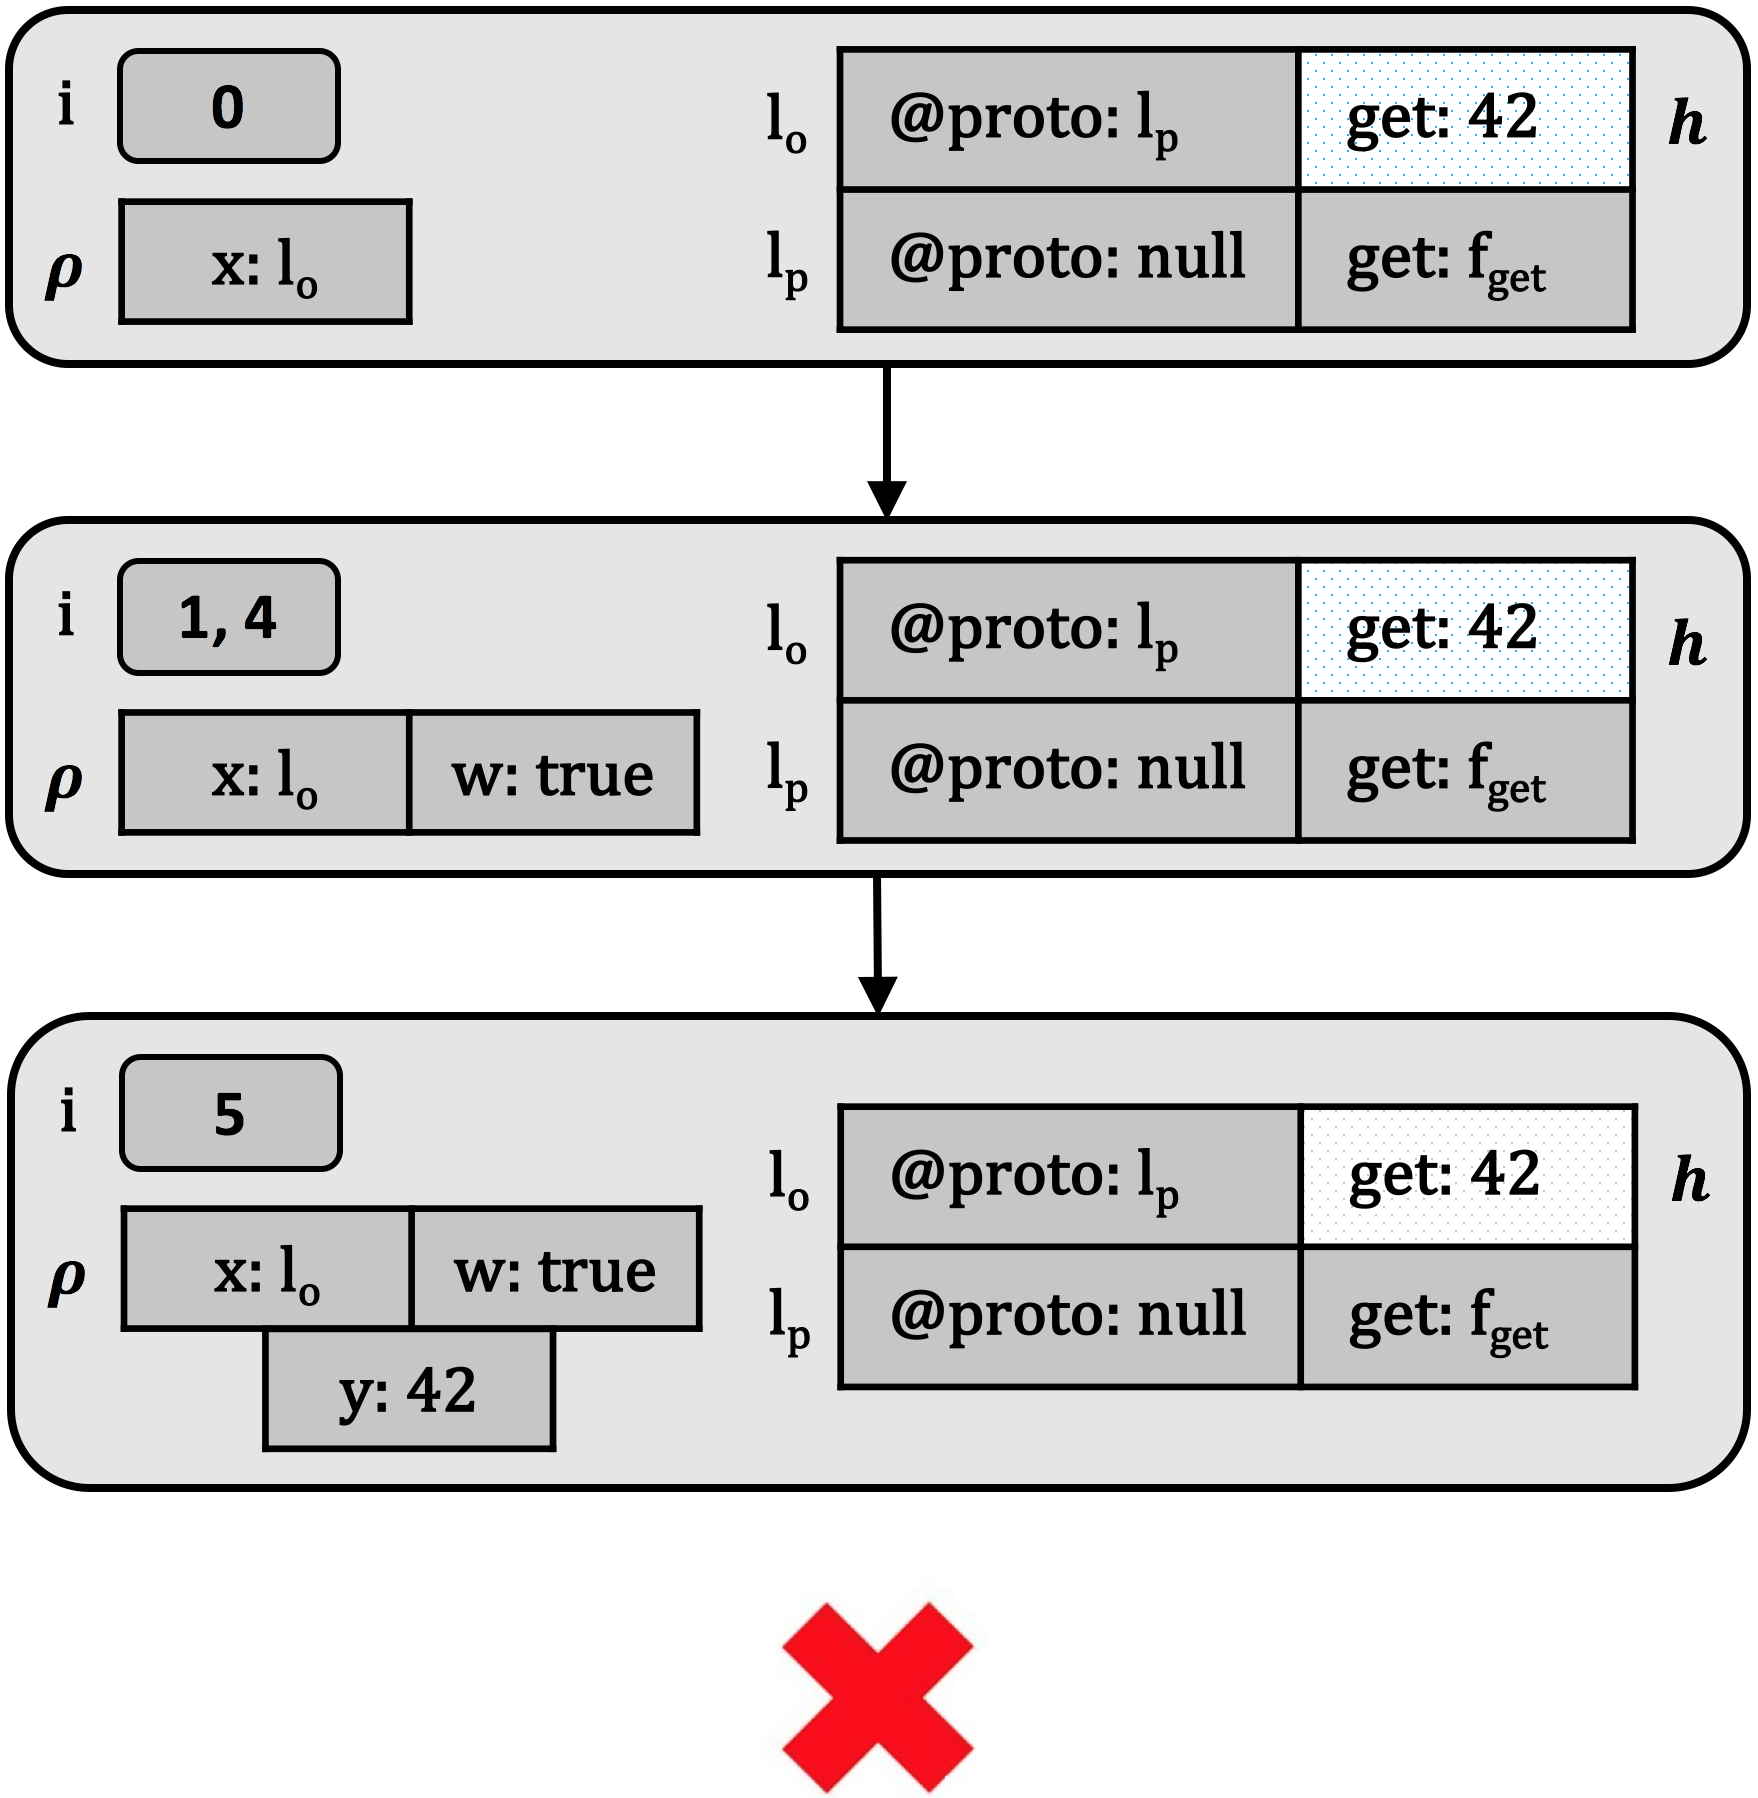
\includegraphics[width=0.265\textwidth,valign=T]{figures/conc_wrong_exec.png}} & & 
{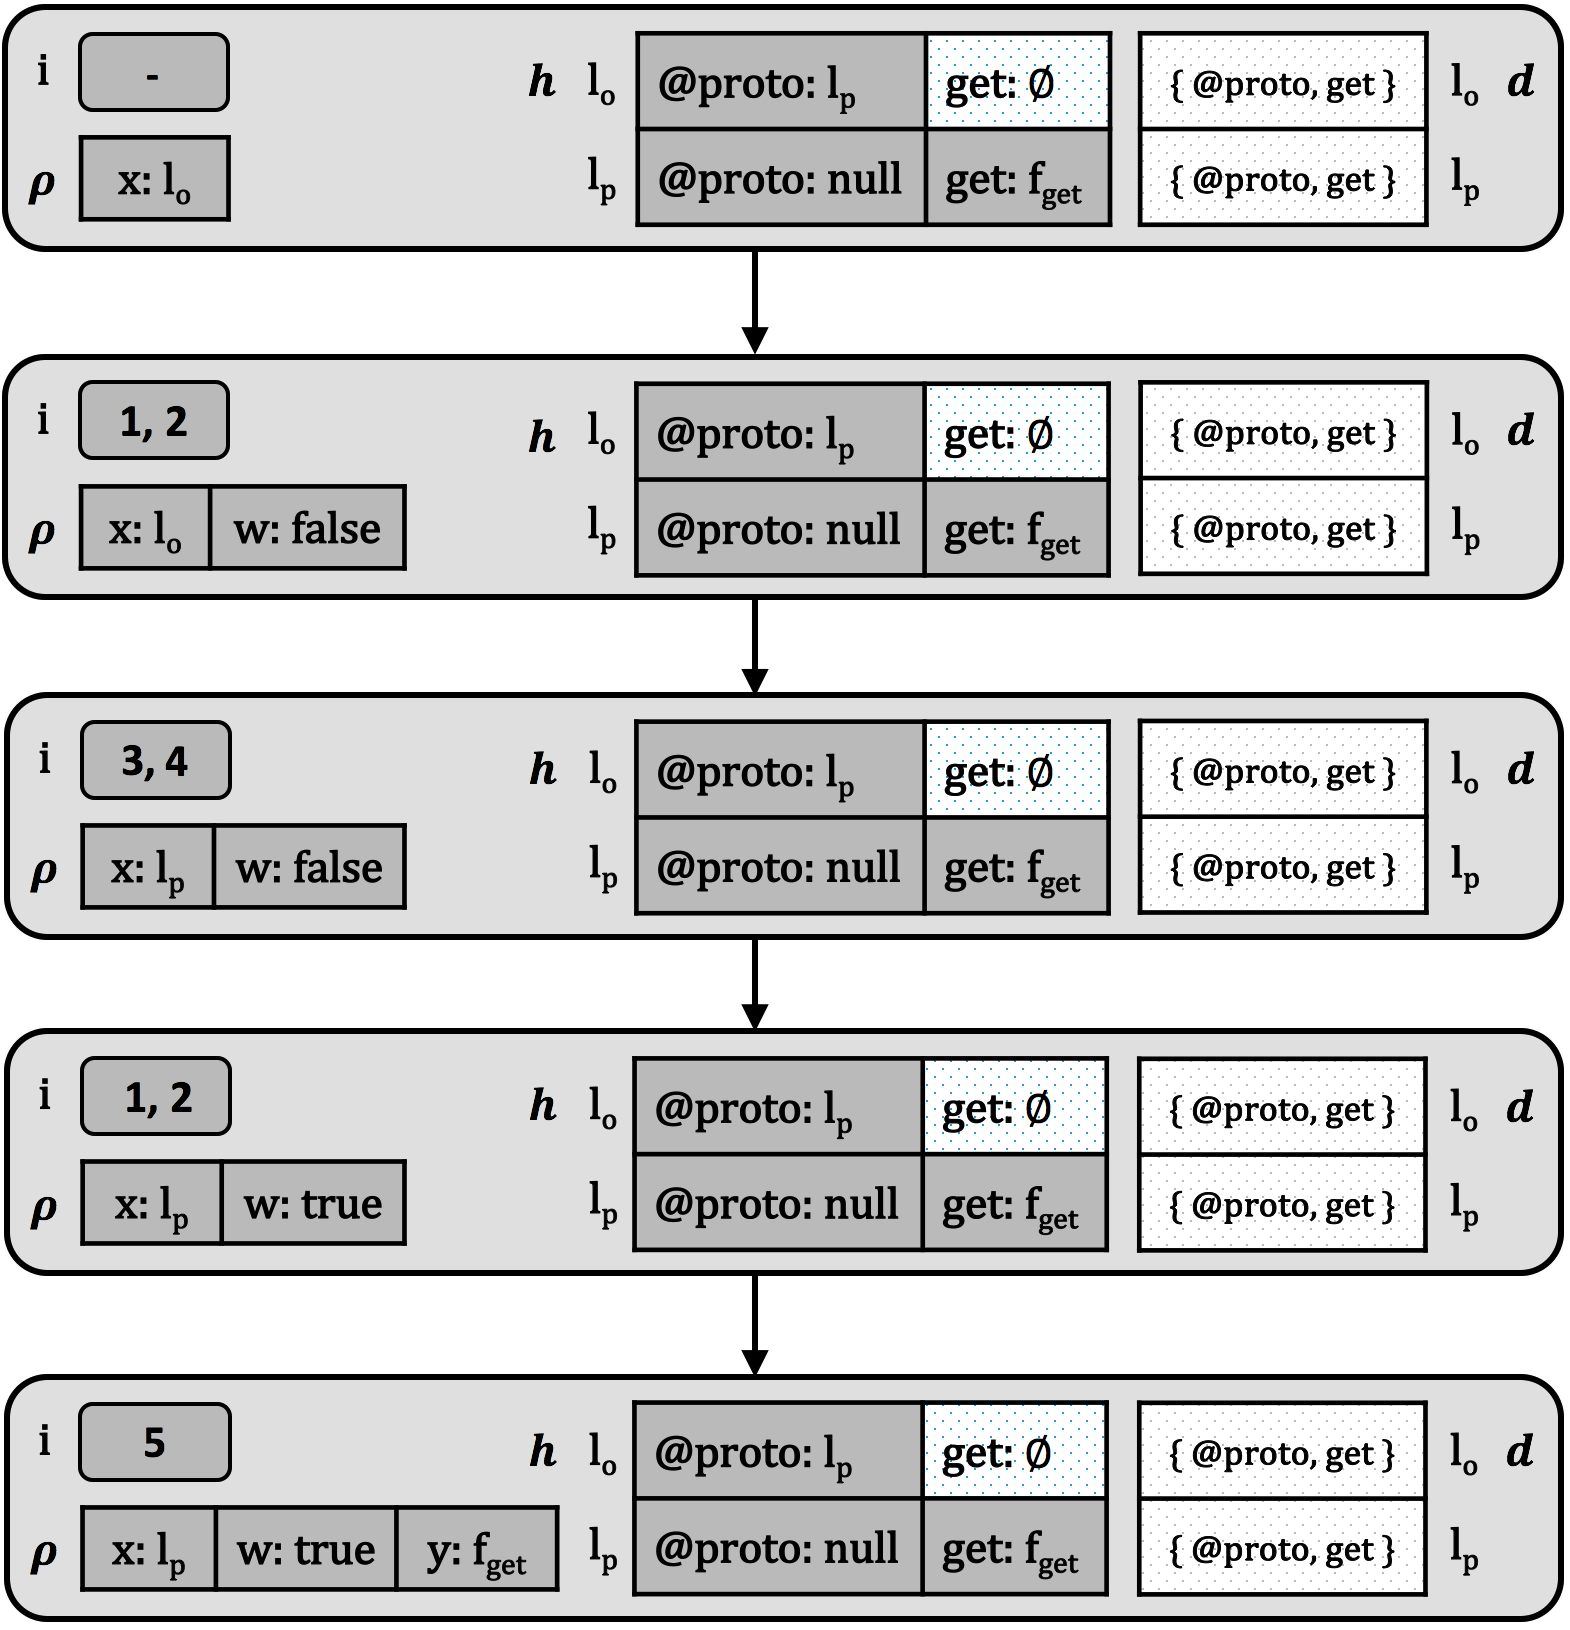
\includegraphics[width=0.347\textwidth,valign=T]{figures/inst_exec.png}}  \\  
\bottomrule
\end{tabular}}
\vspace{2pt}
\caption{Concrete vs. instrumented execution\label{example:symb:states:vs:assertions}}
\vspace*{-0.9cm}
\end{table*}

\begin{figure}[t!]
{\scriptsize
\begin{mathpar} 
\inferrule[\textsc{Basic Command}]
   { 
     \ccmd{\abscs, i} = \bcmd 
     \quad
     \absbsemrule{\absstate, \bcmd}{\absstate'}{} 
   }{\abssemrule{\absstate, \abscs, i}{\absstate', \abscs, i{+}1}{\top}{\top}{}}
   \and 
     \inferrule[\textsc{Goto}]
   { 
   \ccmd{\abscs, i} = \goto \, j \quad}
   {\abssemrule{\absstate, \abscs, i}{\absstate, \abscs, j}{\top}{\top}{}}
   \\
   %
  \inferrule[\textsc{Cond. Goto - True}]
   { \ccmd{\abscs, i} =  \ifgoto{\jsilexpr}{j}{k} 
     %\quad
     %   \absval = \evalexpr{}(\absstate.\stosel, \jsilexpr)
     %   \quad 
     %\absstate' = \absassume{}(\absstate, \jsilexpr) 
   }
   {\abssemrule{\absstate, \abscs, i}{\absassume{}(\absstate, \jsilexpr), \abscs, j}{\top}{\top}{}}
  %
  \qquad
  % 
  \inferrule[\textsc{Cond. Goto - False}]
   { \ccmd{\abscs, i} =  \ifgoto{\jsilexpr}{j}{k} 
      %\quad 
       % \absval = \evalexpr{}(\absstate.\stosel, \jsilexpr)
       % \quad 
      %\absstate' = \absassume{}(\absstate, \neg\jsilexpr) 
   }
   {\abssemrule{\absstate, \abscs, i}{\absassume{}(\absstate, \neg\jsilexpr), \abscs, k}{\top}{\top}{}}
  %
  \\
   %
   \inferrule[\textsc{Normal Return}]
   {
       \abscs = (-, \absstore', \jvar, i, -) :: \abscs'  
       \quad 
       \absstore = \absstate.\stosel
       \\\\
       \absstate' = \stupdt{}(\absstate[\stosel \mapsto \absstore'], \jvar, \absstore(\retvar))
   }  
   {\abssemrule{\absstate, \abscs, \retlab}{\absstate', \abscs', i}{\top}{\top}{}}
     %
   \qquad 
   %
      \inferrule[\textsc{Error Return}]
   { 
       \abscs = (-, \absstore', \jvar, -, j) :: \abscs'
       \quad 
       \absstore = \absstate.\stosel
       \\\\
        \absstate' = \stupdt{}(\absstate[\stosel \mapsto \absstore'], \jvar, \absstore(\errvar))
   }  
   {\abssemrule{\absstate, \abscs, \errlab}{\absstate', \abscs', j}{\top}{\top}{}}
      \\
    \inferrule[\textsc{Procedure Call}]
   { 
    \ccmd{\abscs, i} =   \jsilcall{\jvar}{\jsilexpr}{\jsilexpr_i \mid_{i = 0}^{n}}{j}
     \quad
     \absstore = \absstate.\stosel 
     \quad
    \evalexpr{}(\absstore, \jsilexpr) =  \pid' 
        \quad
     \args(\pid') = \jsillist{\jvar_1, ..., \jvar_{m}} 
      \\\\
      \absval_i = \evalexpr{}(\absstore, \jsilexpr_i) \mid_{i = 0}^{n} 
     \and
      \absval_i = \jundefined \mid_{i = n+1}^{m}  
      \and 
      \absstore' = [ \jvar_i \mapsto \absval_i \mid_{i = 0}^{m}]
   }
   {\abssemrule{\absstate, \abscs, i}{\absstate[\stosel \mapsto \absstore'],  (\pid', \absstore, \jvar, i{+}1, j) :: \abscs, 0}{\top}{\top}{}}
    \\
%
\inferrule[\textsc{Assume}]
  { 
      \ccmd{i}  = \assume(\jsilexpr) 
      \\\\ 
     \absstate' = \absassume{}(\absstate, \jsilexpr) 
  }{\abssemrule{\absstate, \abscs, i}{\absstate', \abscs, i{+}1}{\top}{\top}{}} 
\qquad
\inferrule[\textsc{Assert - True}]
  { 
      \ccmd{\abscs, i}  = \jassert(\jsilexpr)
      \\\\ 
      %\absstore = \absstate.\stosel
      %\quad
      %\absval = \evalexpr{}(\absstore, \jsilexpr)
      % \\\\
       \abssat{}(\absstate, \neg \jsilexpr) = \jfalse
  }{\abssemrule{\absstate, \abscs, i}{\absstate, \abscs, i{+}1}{\top}{\top}{}} 
\qquad 
\inferrule[\textsc{Assert - False}]
  { 
      \ccmd{\abscs, i}  = \jassert(\jsilexpr)
      \\\\ 
      %\absstore = \absstate.\stosel
      %\quad
      %  \absval = \evalexpr{}(\absstore, \jsilexpr)
      % \\\\
      \abssat{}(\absstate, \neg \jsilexpr) = \jtrue
  }{\abssemrule{\absstate, \abscs, i}{\absstate, \abscs, i}{\top}{\bot}{}} 
 \end{mathpar}}
 \vspace*{-0.52cm}
 \captionsetup{format=nastyCaption}
\caption*{{\small Figure 4. Abstract semantics, commands: $\abssemrule{\absstate, \abscs, i}{\absstate', \abscs', j}{\mode}{\mode'}{}$}}\label{abs:sem:cmds:fig}
\vspace*{-0.6cm}
\end{figure}

\vspace*{-0.2cm}
\subsection{\jsil Concrete Semantics}
\label{subsec:concr}
A \jsil concrete state $\jstate$ is a pair $(\heap, \store)$, consisting of a heap and a store. 
A heap, $\heap \in \heaps$, is a partial function mapping pairs of  object locations and property names (strings) to \jsil values.
A store, $\store \in \stores$, maps program variables to \jsil values. 
In the following, we denote a heap cell by $\hcell{\loc}{\jstring}{\val}$, meaning that $\heap(\loc, \jstring) = \val$.

We instantiate the abstract semantics for the concrete case by providing the appropriate definitions 
for the required abstractions.
%, noting that abstract values are instantiated to\jsil values extended with the property absence indicator $\none$.
We write $\absbsemrule{\jstate, \bcmd}{\jstate'}{\concrete}$ for the concrete semantic 
judgement for \jsil basic commands and $\abssemrule{\jstate, \cs, i}{\jstate', \cs', j}{\mode}{\mode'}{\concrete}$ 
for \jsil commands. 

The instantiation of the \jsil abstract semantics to the concrete case is straightforward: if an object \jsinline|l| has property \jsinline|p|, GetCell returns the associated value, and $\none$ otherwise; GetDomain returns the set of properties of a given object;
heap allocation returns a fresh object location without changing the state;
the rules for store update and positive heap update are standard; and 
the negative heap update removes the given property of a given object from the heap.
Note that the positive and negative heap update rules are not applicable at the same time, as $\val$ cannot be equal to $\none$. 

\smallskip
\begin{display}{Selected Concrete Semantics Rules}
\text{
{\scriptsize
\begin{mathpar} 
%  \inferrule[\textsc{Expression Evaluation}]
%  {}{\evalexpr{\concrete}(\store, \val) = \val \qquad 
%  	\evalexpr{\concrete}(\store, \jvar) = \store(\jvar) \qquad 
%	\evalexpr{\concrete}(\store, \ominus \jsilexpr) = \semop{\ominus} \ \evalexpr{c}(\store, \jsilexpr) \qquad
%	\evalexpr{\concrete}(\store, \jsilexpr_1 \oplus \jsilexpr_2) = \evalexpr{c}(\store, \jsilexpr_1) \ \semop{\oplus} \ \evalexpr{c}(\store, \jsilexpr_2)}
%  \\
    %
        \inferrule[\textsc{GetCell - Found}]
   { 
         \loc = \evalexpr{\concrete}(\store, \jsilexpr_1) 
        \quad 
         p = \evalexpr{\concrete}(\store, \jsilexpr_2) 
        \\\\
       \heap = - \, \uplus \, (\loc, p) \mapsto \val
       \quad 
       r = (\loc, p, \val)
        }{  \absgetcellrule{\concrete}{(\heap, \store), \jsilexpr_1, \jsilexpr_2}{(\heap, \store), r}}
        \qquad
    \inferrule[\textsc{GetCell - Not Found}]
   { 
         \loc = \evalexpr{\concrete}(\store, \jsilexpr_1) 
        \quad 
         p = \evalexpr{\concrete}(\store, \jsilexpr_2) 
        \\\\
       (\loc, p) \not\in \domain(\heap)
       \quad 
       r = (\loc, p, \none)
        }{  \absgetcellrule{\concrete}{(\heap, \store), \jsilexpr_1, \jsilexpr_2}{(\heap, \store), r}}
  %
  \\
  \inferrule[\textsc{GetDomain}]
   { 
       \loc = \evalexpr{\concrete}(\store, \jsilexpr) 
      \quad (\loc,-) \notin \domain (\heap') \\\\
       \heap = \heap' \, \uplus \, \big((\loc, p_i) \mapsto \val_i \big)\mid_{i = 0}^m  
       }{  \absgetdomainfun{\concrete}((\heap, \store), \jsilexpr) \semeq \jsilset{p_1, ..., p_m}}
  %
 %
 \quad 
    \inferrule[\textsc{Heap Alloc.}]
   { %\loc \text{ fresh } 
       \jstate = (\heap, -) \\\\
       %
       (\loc, -) \not\in \domain(\heap)
   }{
   \absalloc{c}(\absstate) =  (\loc, \jstate)}
   \quad
   \inferrule[\textsc{Store Update}]
   { 
         \store' = \store[\jvar \mapsto \val]
   }{  \stupdt{\concrete}((\heap, \store), \jvar, \val) =  (\heap, \store')}
   \\ 
       \inferrule[\textsc{Positive Heap Update}]
   { 
         \heap' = \heap[(\loc, p) \mapsto \val]
         %\quad 
      %  {\color{red} \val \neq \none}
   }{  \hpupdt{\concrete}((\heap, \store), \loc, p, \val) \semeq  (\heap', \store)}
 \qquad
       \inferrule[\textsc{Negative Heap Update}]
   { 
         \heap = \heap' \dunion (\loc, p) \mapsto -
   }{  \hpupdt{\concrete}((\heap, \store), \loc, p, \none) \semeq  (\heap', \store)}
%   \\\\
%      \inferrule[\textsc{Expr - SymbVar}]
%   {\svar \in \svars \text{ is of type } \jtype \\\\
%   \val \in \vals \text{ is of type } \jtype
%   }{\evalexpr{\concrete}(-, \svar) \semeq \val}
    
%  \inferrule[\textsc{Assume}]
%   {
%       \evalexpr{\concrete}(\jstate.\stosel, \jsilexpr) = \jtrue
%   }{  \absassume{\concrete}(\jstate, \jsilexpr) \semeq  \jstate }
%  	\and
%    \inferrule[\textsc{Check Sat}]
%   {
%        \jbool = \evalexpr{\concrete}(\jstate.\stosel, \jsilexpr) 
%   }{  \abssat{\concrete}(\jstate, \jsilexpr) \semeq \jbool}
  \end{mathpar}
  }}
 \end{display}

%The remaining rules can be seen in the Appendix.

%\jfs{
%\begin{itemize}
%   %\item mention the missing rules
%   \item explain the two getcell rules 
%   %\item explain the symbols that are not defined
%\end{itemize}
%}


\begin{wrapfigure}{R}{0.13\textwidth}
\vspace*{-0.2cm}
{\footnotesize
\hspace*{-0.47cm} $\mathtt{1\quad w := \hasfield(x, \litstring{get})}$ \\[-0.08cm]
\hspace*{-0.47cm} $\mathtt{2\quad \ifgoto{w}{5}{3}}$ \\[-0.08cm]
\hspace*{-0.47cm} $\mathtt{3\quad x := [x, \litstring{\protop}] }$ \\ [-0.08cm]
\hspace*{-0.47cm} $\mathtt{4\quad \ifgoto{x = \jnull}{\errlab}{1}}$ \\[-0.08cm]
\hspace*{-0.47cm} $\mathtt{5\quad y := [x, \litstring{get}]}$ \\[-0.08cm]
\hspace*{-0.47cm} $\mathtt{6\quad \jsilcall{z}{y}{}{\errlab}}$ 
}
\vspace*{-0.2cm}
%{\hspace*{-1cm}{\mbox{\caption{\jsil Example 1\label{jsil:example:frame}}}}}
\end{wrapfigure}



\smallskip
\myparagraph{Example: Frame}
The \jsil concrete semantics does not satisfy the frame property. 
We illustrate this with the program on the right, which 
looks for the property $\litstring{get}$ in the 
prototype chain of the object bound to $\mathtt{x}$, reads the value of that 
property, and calls the procedure whose identifier is bound to that value. 
The program terminates successfully when run from the state 
described in the top left corner of Table~\ref{example:symb:states:vs:assertions}. However, if we extend the initial state with the frame $(\loc_o, \litstring{get}) \mapsto 42$, 
as shown in the second column of Table~\ref{example:symb:states:vs:assertions}, the procedure 
call fails, as $42$ is not a procedure identifier. 

\vspace*{-0.2cm}
\subsection{\jsil Instrumented Semantics}\label{subsec:instrumented}


%Our instrumented semantics explicitly keeps track of properties that are not present in a given object, using ideas from~\cite{gardner:popl:2012,javert}.

Compositional analyses must reason about programs given partial state information.
This is particularly challenging for languages that do not observe the frame property.
We approach this problem by first designing an instrumented version of the language semantics that \emph{does} 
observe the frame property. 
%
To achieve this, the \jsil instrumented semantics keeps track of both the present \emph{and the absent} properties of a given object, 
using ideas from~\cite{gardner:popl:2012,javert}.

An instrumented state $\istate$ is a triple $(\iheap, \idom, \store)$ consisting of an instrumented heap, 
a domain table, and a store. 
%
An instrumented heap, $\iheap \in \iheaps : \locs \partialmap \strings \partialmap \setext{\vals}{\none}$, 
differs from a concrete heap in that it can map object properties to $\none$, explicitly declaring their absence. 
We refer to those cells as \emph{$\none$-cells} (read: none-cells). 
%
A domain table, $\idom : \locs \partialmap \vals$, maps object locations to sets of properties that the corresponding objects may have, whereas all other properties are \emph{known to be} absent. If $\idom(\loc)$ is defined and if $p \not\in \idom(\loc)$, then we know that the object at $\loc$ \emph{does not have} the property~$p$, and that that property \emph{cannot} be framed on. In contrast, any properties in $\idom(\loc)$ that are not in the heap can be safely framed on. Also, if we have that $(\loc, p) \in \domain(\iheap)$, then it holds that $p \in \idom(\loc)$.
On the other hand, if $\idom(\loc)$ is not defined, then all properties of the object at $\loc$ that are not in the heap \emph{can be} safely framed~on.

%We also know that all of the 
%properties of that object that are in the heap are also in $\idom(\loc)$.
%In this way, we implicitly keep track of an infinite number of absent properties.

We instantiate the abstract semantics to the instrumented case. 
We write $\absbsemrule{\istate, \bcmd}{\istate'}{\instrumented}$ for the instrumented semantic 
judgement for basic commands, and $\abssemrule{\istate, \cs, i}{\istate', \cs', j}{\mode}{\mode'}{\instrumented}$ 
for~commands. The omitted rules coincide with the concrete case. 

\begin{display}{Selected Instrumented Semantics Rules}
\text{
{\scriptsize
\begin{mathpar} 
     \inferrule[\textsc{Heap Update}]
   { 
         \istate = (\iheap, \idom, \store) 
         \quad
         \iheap' = \iheap[(\loc, p) \mapsto \ival]
   }{  \hpupdt{\instrumented}(\istate, (\loc, p), \ival) =  (\iheap', \idom, \store) }
   \and
      \inferrule[\textsc{GetCell - Found}]
   { 
        \istate = (\iheap, -, \store) 
        \quad
         \loc = \evalexpr{\concrete}(\store, \jsilexpr_1) 
      \\\\
         p = \evalexpr{\concrete}(\store, \jsilexpr_2) 
         \quad 
       \iheap = - \, \uplus \, (\loc, p) \mapsto \ival
        }{  \absgetcellrule{\instrumented}{\istate, \jsilexpr_1, \jsilexpr_2}{\istate, (\loc, p, \ival)}}
        \\
 % 
     \inferrule[\textsc{GetCell - Not Found}]
   { 
        \loc = \evalexpr{\concrete}(\store, \jsilexpr_1) 
        \quad 
         p = \evalexpr{\concrete}(\store, \jsilexpr_2) 
         \quad
         p \not\in \idom(\loc) 
         \quad
         \iheap' = \iheap \dunion (\loc, p) \mapsto \none
         \quad
         \idom' = \idom[\loc \mapsto \idom(\loc) \cup \jsilset{p}]
            }{  \absgetcellrule{\instrumented}{(\iheap, \idom, \store), \jsilexpr_1, \jsilexpr_2}{(\iheap', \idom', \store), (\loc, p, \none)}}
  %
  \\
  \inferrule[\textsc{GetDomain}]
   { 
       \loc = \evalexpr{\concrete}(\store, \jsilexpr) 
      \and
       \iheap = \iheap' \, \uplus \, \big((\loc, p_i) \mapsto - \big)\mid_{i = 0}^m  
        \and
        %
          (\loc,-) \notin \domain (\iheap')  
        \\\\
          \jsilset{p_1, ..., p_m} = \idom(\loc)
          \and
        \forall_{0 \leq i \leq n} \, \val_i \neq \none 
         \and 
           \forall_{n < i \leq m} \, \val_i = \none 
   }{  \absgetdomainfun{\instrumented}((\iheap, \idom, \store), \jsilexpr) \semeq \jsilset{p_1, ..., p_n}}
 %
 % 
 \end{mathpar}}}
 \end{display}
 
 
\setcounter{figure}{4}   
\begin{figure*}[!t]
\centering
\begin{tabular}{c||c}
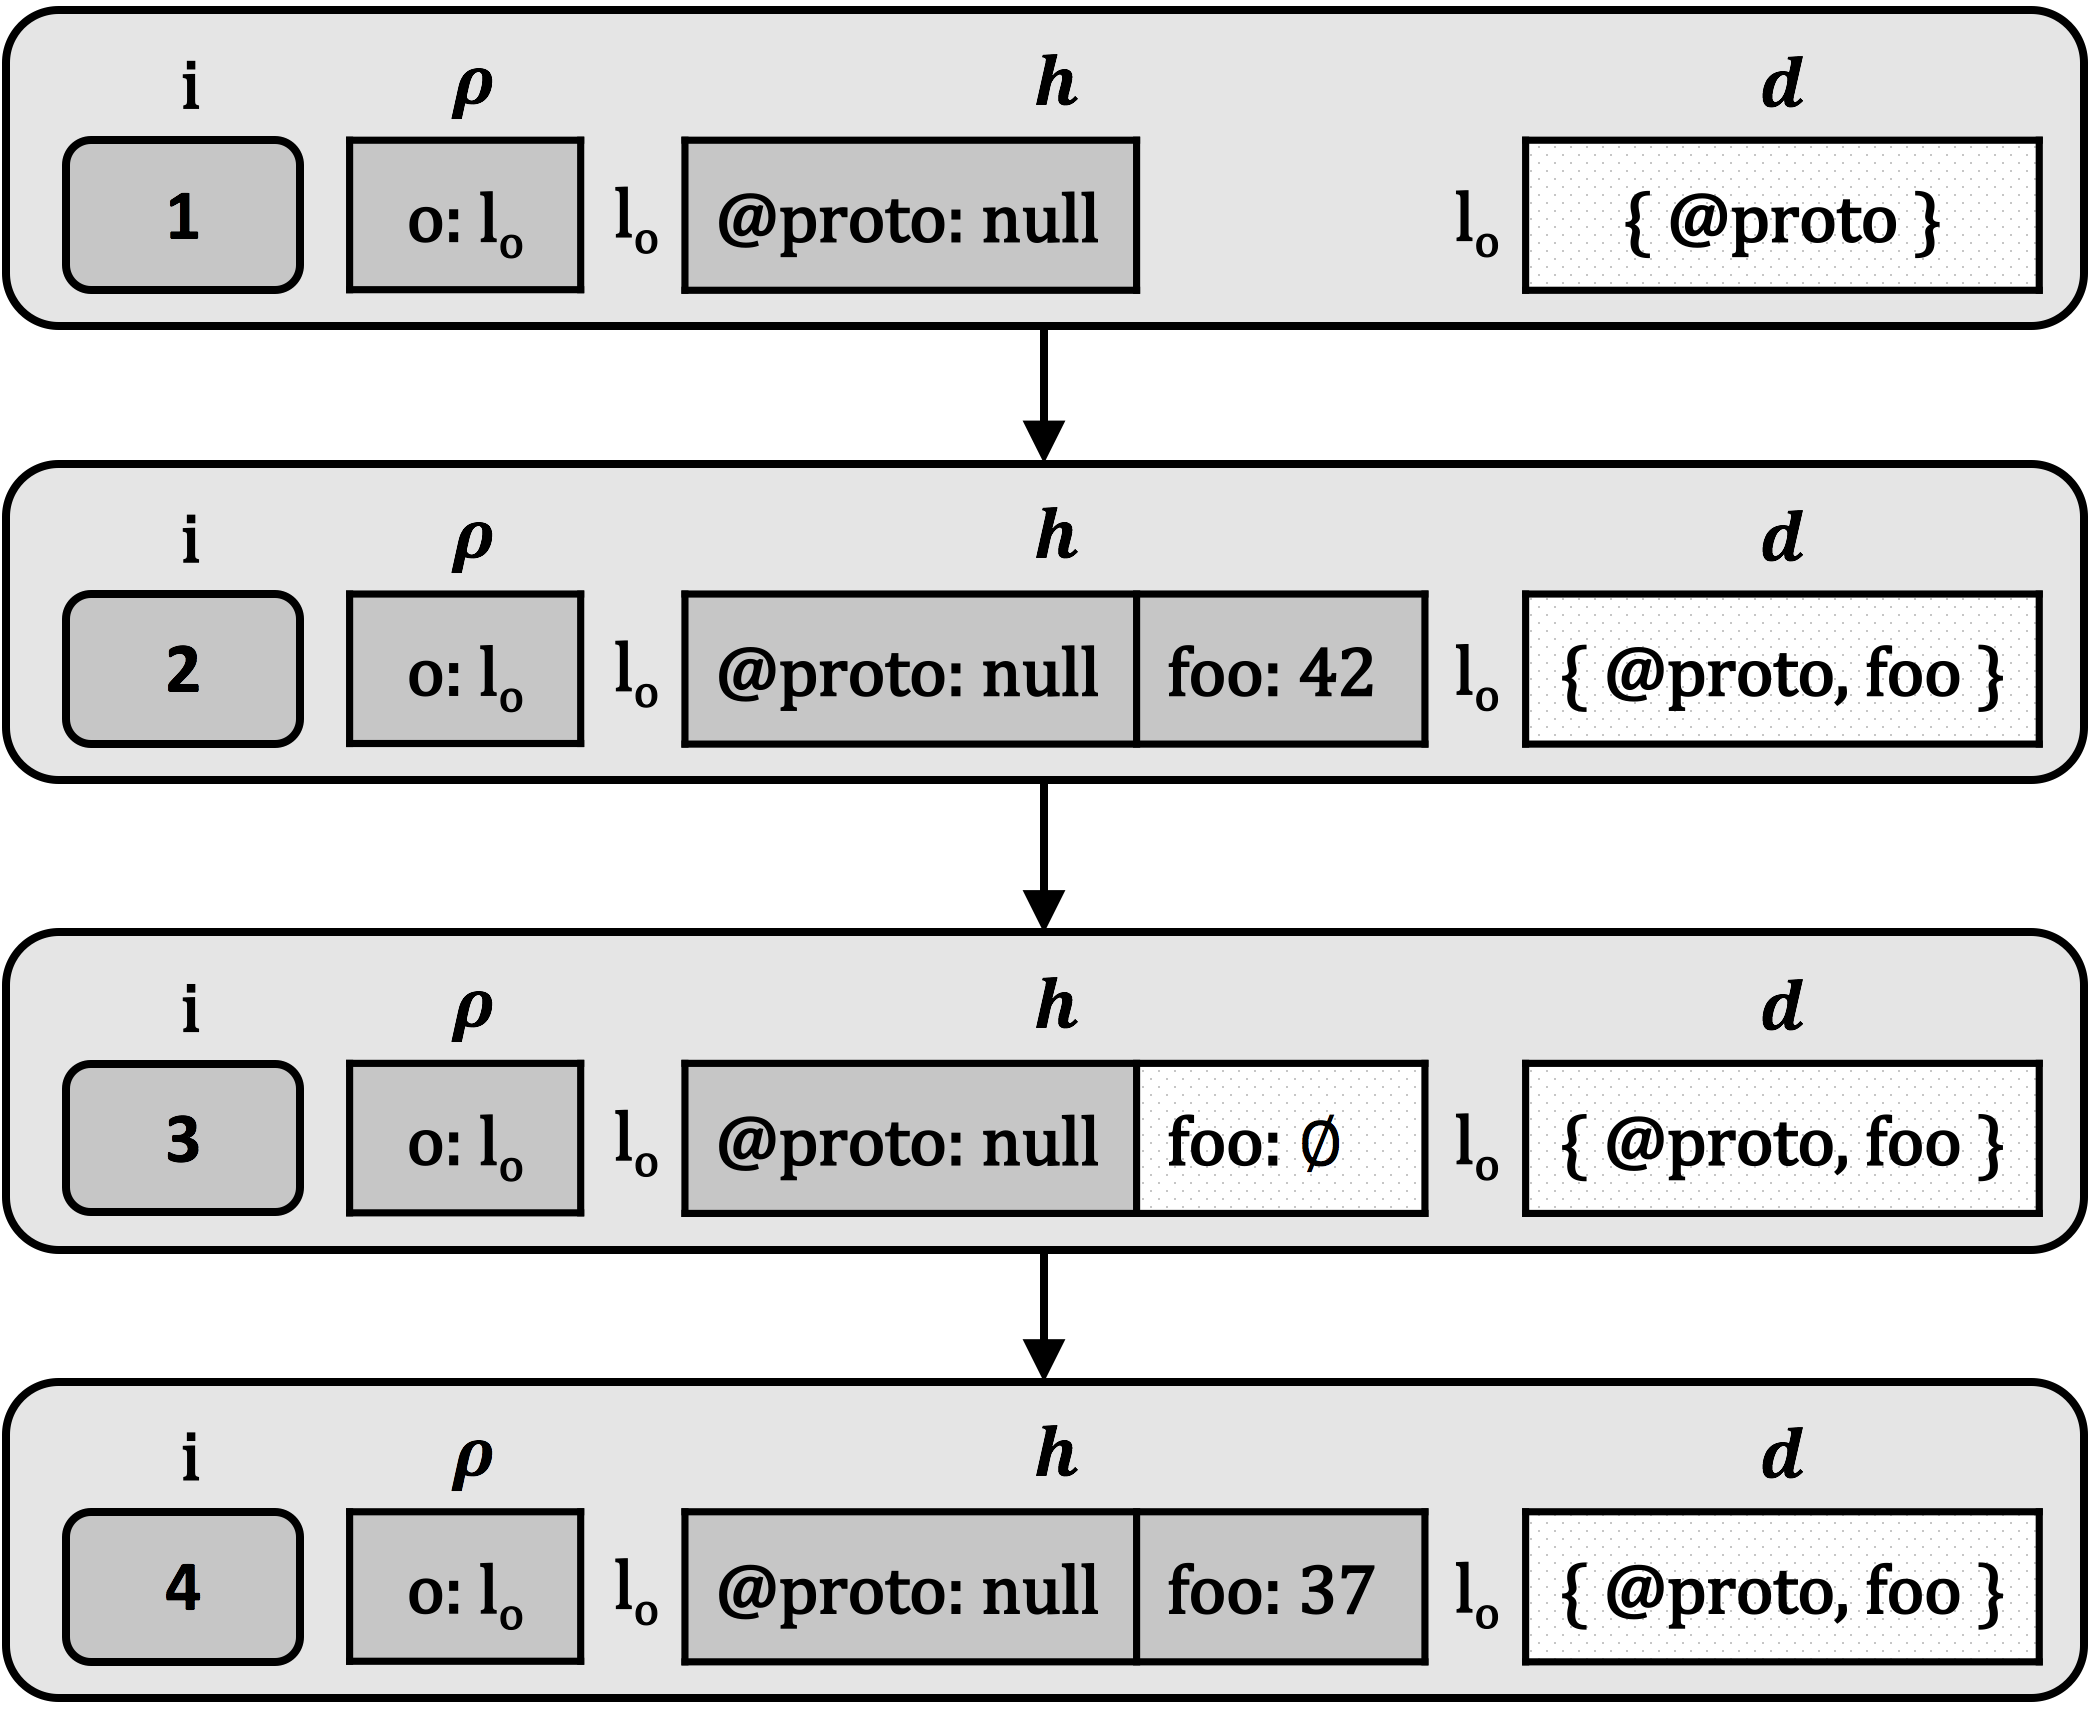
\includegraphics[width=0.28\textwidth]{figures/domaintable.png} \ & \ 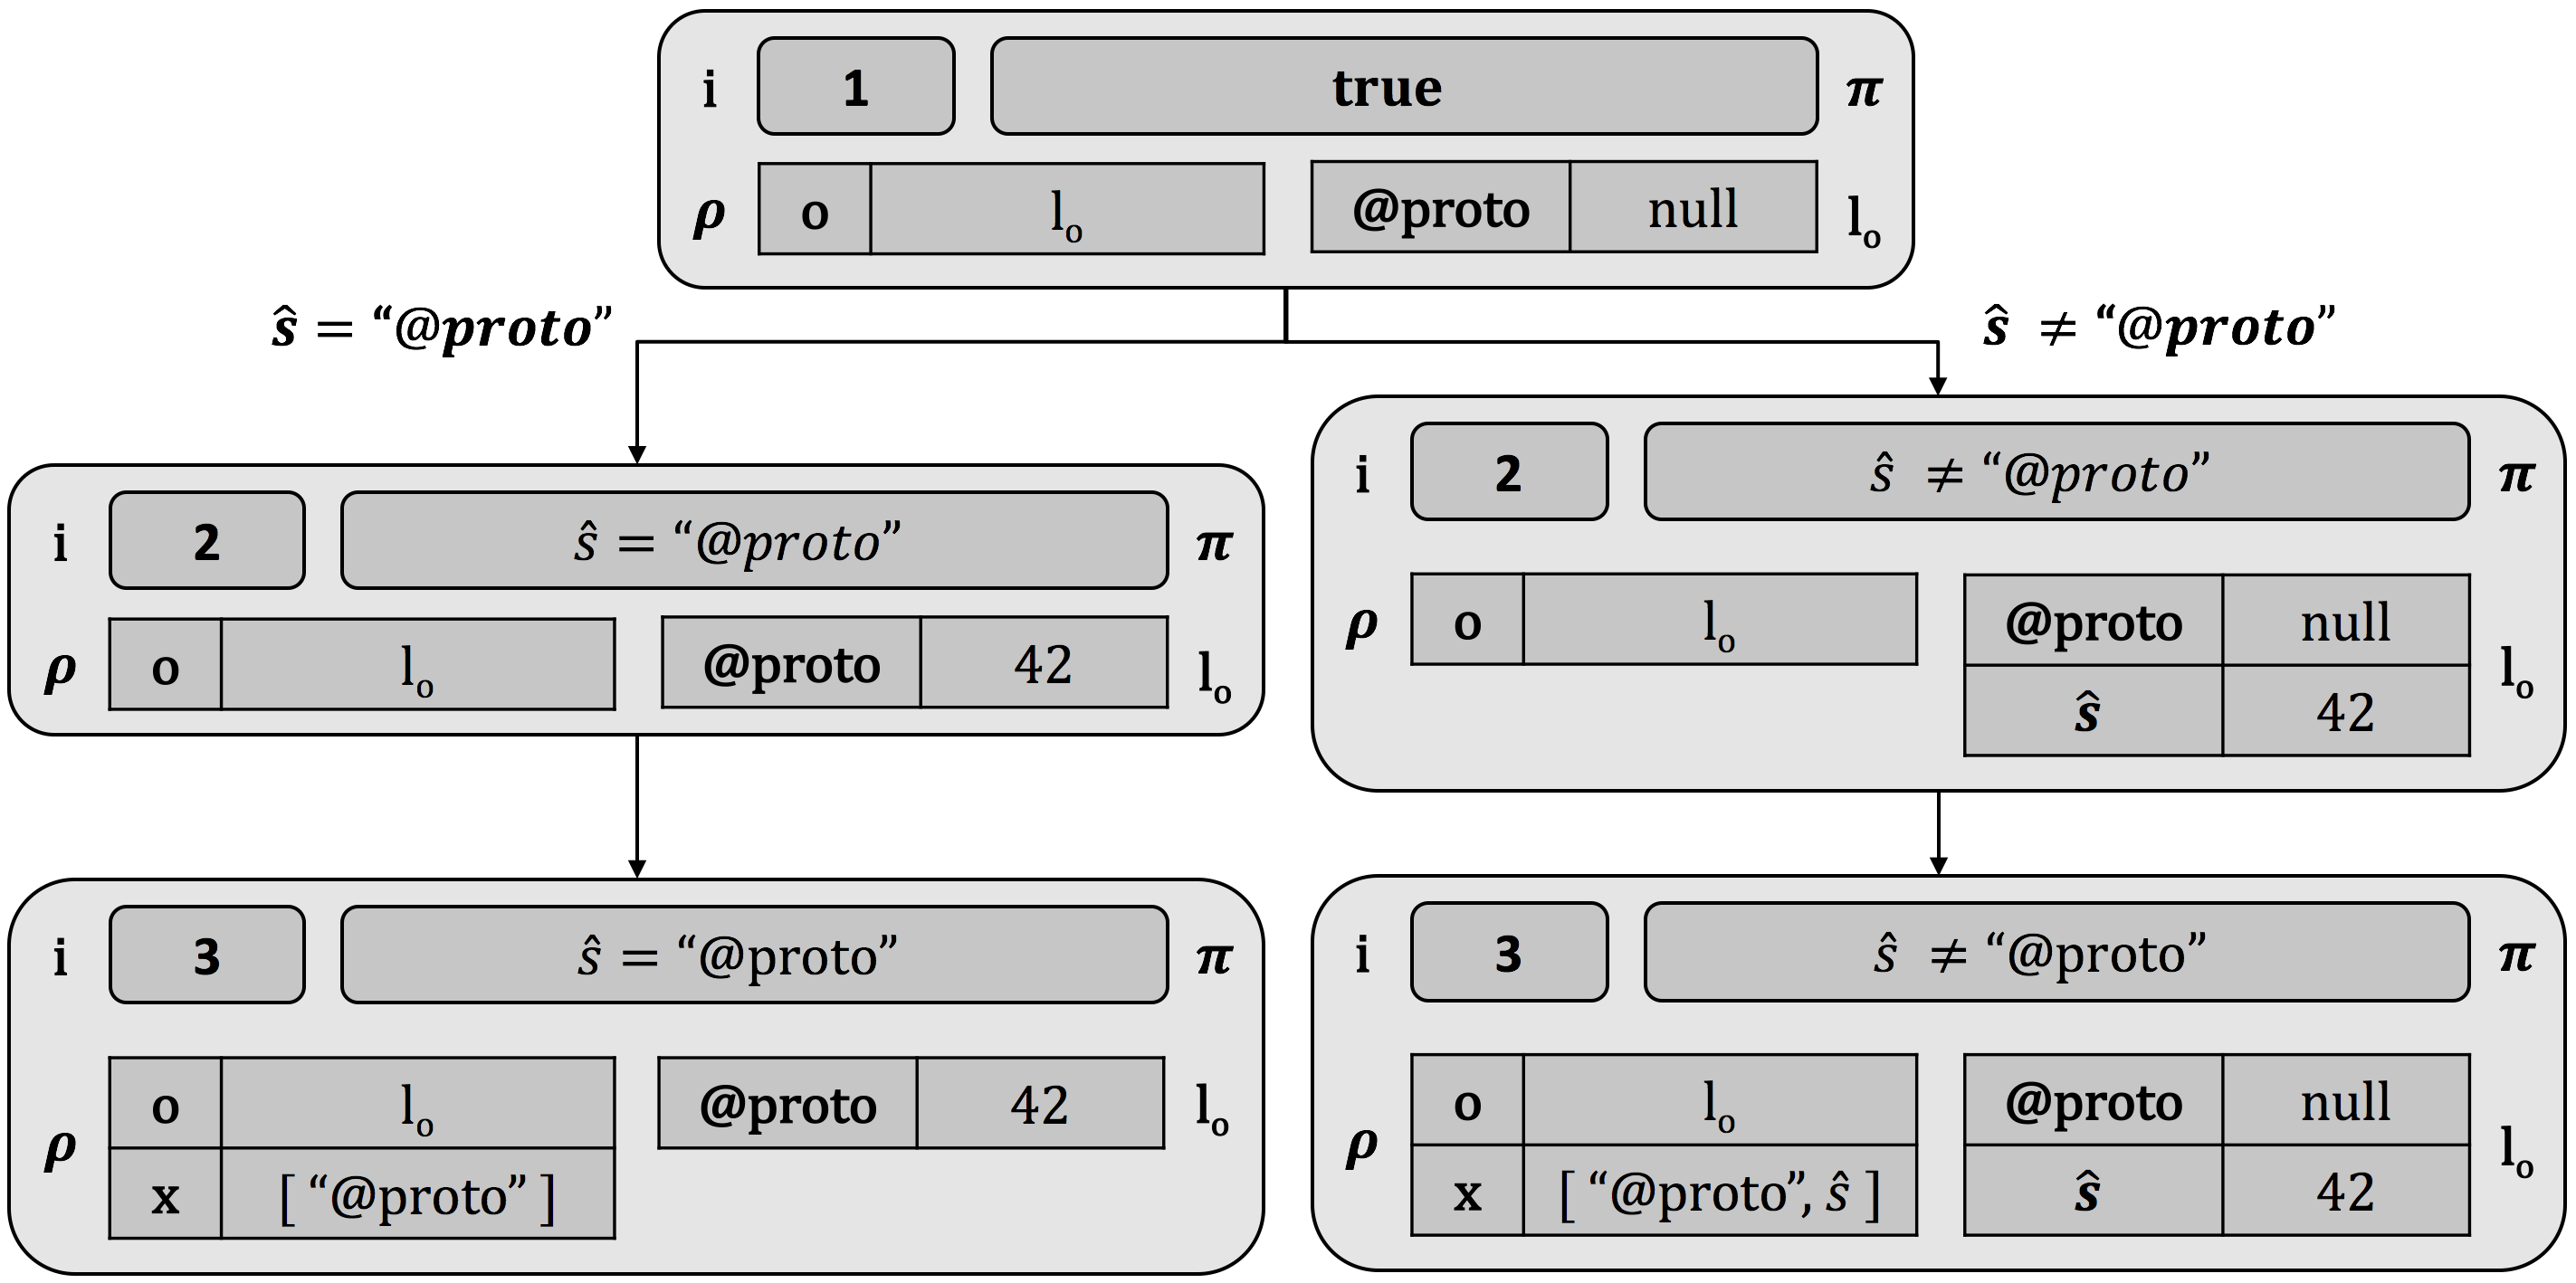
\includegraphics[width=0.59\textwidth]{figures/symbSemEx.png}
\end{tabular}
\vspace*{-0.3cm}
\caption{Execution traces: Instrumented GetCell (left); Symbolic branching (right)}
\label{fig:sexecexample}
\vspace*{-0.4cm}
\end{figure*}


As $\ival$ ranges over $\setext{\vals}{\none}$, the \textsc{Heap Update} rule may update the value of an object property to $\none$.  
In the concrete case, the corresponding rule would simply remove that property from the heap.  
 As an instrumented heap can contain $\none$-cells, the \textsc{GetDomain} rule has to filter out properties mapped to $\none$. 
 Furthermore, in order to apply this rule, one has to have full information about the object: all properties from $\idom(\loc)$ must be present in the heap. 
 %note how GetDomain collects all non-none properties of an object by inspecting both the heap and the domain table. 
%
Another difference between the two semantics is apparent in the rule \textsc{GetCell - Not Found}: while $\absgetcellrule{\instrumented}{\istate, \jsilexpr_1, \jsilexpr_2}{-, (-, -, \none)}$ 
means that one is certain that the object denoted by $\jsilexpr_1$ does not have the property 
denoted by $\jsilexpr_2$, $\absgetcellrule{\concrete}{\jstate, \jsilexpr_1, \jsilexpr_2}{-, (-, -, \none)}$ 
only means that this property does not exist in the current heap. %(and might be later framed on). 
%
%We note that the instrumented semantics does not evaluate symbolic variables.

 
 %As we inspect properties using GetCell, they .
 
 \myparagraph{Example: Frame revisited}
 In the rightmost column of Table~\ref{example:symb:states:vs:assertions}, we give the instrumented 
 execution of the frame example when
 the object at location $l_o$ is guaranteed not to have the property $\litstring{get}$. 
 Then, the  instrumented heap cannot be extended  with 
 the frame $(\loc_o, \litstring{get}) \mapsto 5$ as it overlaps with $(\loc_o, \litstring{get}) \mapsto \none$, meaning 
 that the illustrated frame bug cannot be replicated in the instrumented setting.  
 Also, if we remove $(\loc_o, \litstring{get}) \mapsto \none$ from the initial heap, 
 the instrumented execution will get stuck in the execution of line~$0$. 

\begin{wrapfigure}{R}{0.11\textwidth}
\vspace*{-0.3cm}
{\footnotesize
\hspace*{-0.5cm} $\mathtt{1\quad o := \jsilnew ()}$ \\[-0.06cm]
\hspace*{-0.5cm} $\mathtt{2\quad [o, \litstring{foo}] := 42}$ \\[-0.06cm]
\hspace*{-0.5cm} $\mathtt{3\quad \jsildelete(o, \litstring{foo})}$ \\ [-0.06cm]
\hspace*{-0.5cm} $\mathtt{4\quad [o, \litstring{foo}] := 37}$ 
}
\vspace*{-0.4cm}
%{\hspace*{-1cm}{\mbox{\caption{\jsil Example 1\label{jsil:example:frame}}}}}
\end{wrapfigure}

\myparagraph{Example: Instrumented GetCell}
To better understand the interaction between GetCell, the heap, and the domain table, consider the 
 program on the right and its execution trace in Figure~\ref{fig:sexecexample} (left). When executing the first property assignment, following the abstract \textsc{Property Assignment} rule, we must call $\getcell(\mathtt{o, \litstring{foo}})$ to obtain the current value of the property. As the property is not in the heap, we are in the \textsc{Not Found} case of GetCell. The domain is extended with $\litstring{foo}$, and the heap is extended with the none-cell $\mathtt{(\loc_o, \litstring{foo})} \mapsto \none$, whose value is then updated to 42 by the heap update. After the deletion, its value is reset to $\none$. The following property assignment will again call $\getcell(\mathtt{o, \litstring{foo}})$, but this time, we will be in the \textsc{Found} case of GetCell, as the property is in the heap.
In a nutshell, GetCell ensures that all inspected properties, both present and absent, are represented in the heap.

%\jfs{
%\begin{itemize}
%  \item An example to explain the domain and how it interacts with the none-fields
%\end{itemize}
%}



\myparagraph{Formal Guarantees}
Theorem~\ref{teo:frame:property} states that the \jsil instrumented semantics observes the 
frame property. Lemma~\ref{lemma:instrumented:semantics} relates the instrumented 
semantics with the concrete semantics via an erasure function  $\interpret{\instconc}{}$. Informally, $\interpret{\instconc}{}(\istate)$
denotes the concrete state obtained by erasing negative information in $\istate$ (i.e.,~  
$\none$-cells and domain information). 
Lemma~\ref{lemma:instrumented:semantics} states that if a given execution 
goes through in the instrumented semantics, then its concretisation (given by $\interpret{\instconc}{}$) 
goes through in the concrete semantics. %All proofs can be found in the Appendix.
For $\istate = (\iheap, \idom, \store)$, we write $\istate \dunion \iheap'$ to denote $(\iheap \dunion \iheap', \idom, \store)$ defined only when $\iheap'$ does not redefine the properties stated not to exist by the domain table $\idom$.

\begin{theorem}[Frame Property - Instrumented Semantics]\label{teo:frame:property}
\hspace*{-0.28cm}$$
\transabssemrule{\istate, \cs, i}{\istate', \cs', j}{\mode}{\mode'}{\instrumented}\Rightarrow
        \transabssemrule{\istate \dunion \iheap_f, \cs, i}{\istate' \dunion \iheap_f, \cs', j}{\mode}{\mode'}{\instrumented} 
$$
\end{theorem}

\begin{lemma}[Transparency for Instrumentation]\label{lemma:instrumented:semantics}
$$
\hspace*{-0.22cm}
\transabssemrule{\istate, \cs, i}{\istate', \cs', j}{\mode}{\mode'}{\instrumented} \Rightarrow \transabssemrule{\interpret{\instconc}{}(\istate), \cs, i}{\interpret{\instconc}{}(\istate'), \cs', j}{\mode}{\mode'}{\concrete} 
$$
\end{lemma}



%
%\begin{display}{Instrumented State Interpretation}
%{\scriptsize 
%\begin{mathpar}
%\inferrule[Symbolic Heaps]{}{
%\interpret{\instconc}{}(\hemp) \semeq \hemp
%\quad
%\frac{
%   \heap = \hcell{\loc}{p}{\val}
%}{
%\interpret{\instconc}{}(\hcell{\loc}{p}{\val}) \semeq  \heap
%}
%\quad
%  \interpret{\instconc}{}(\hcell{\loc}{p}{\none}) \semeq \hemp }
%\quad
%\frac{
%  \begin{array}{c}
%   \interpret{\instconc}{}(\iheap_i) = \heap_i, \hdom_i \mid_{i =1,2} \\
%   \heap = \heap_1 \dunion \heap_2
%  \end{array}
%}{
%\interpret{\instconc}{}(\iheap_1 \dunion \iheap_2) \semeq  \heap
%}
%\qquad
%\inferrule[Symbolic States]{
%    \interpret{\instconc}{}(\iheap) = \heap
%}{
%\interpret{\instconc}{}(\iheap, \idom, \store) \semeq (\heap, \store)
%}
%\end{mathpar}}
%\end{display}




\vspace*{-0.2cm}
\subsection{\jsil Symbolic Semantics}\label{subsec:symb:semantics}

We obtain the \jsil symbolic semantics by lifting the \jsil instrumented semantics to the symbolic level, following standard approaches~\cite{Rosette1}.
This lifting, however, is easier for us to achieve because we only need to instantiate the abstract semantics, rather than re-examine every command of the language.

We instantiate the abstract values to \emph{symbolic expressions}, $\sexpr \in \sexprs$, defined as follows: 
$\sexpr \triangleq \val \mid \svar \mid \unoper\ \sexpr \mid \sexpr \binoper \sexpr$. 
For clarity, we use $\sexprp$ for symbolic expressions denoting property names, and $\sexprv$ for symbolic
expressions denoting arbitrary values. 


A \emph{symbolic state}, $\sstate = (\sheap, \sdom, \sstore, \pc)$, consists of a 
symbolic heap~$\sheap$, a symbolic domain $\sdom$, a symbolic store $\sstore$, and a path condition~$\pc$. 
The symbolic heap, symbolic domain, and symbolic store are obtained from their instrumented 
counterparts of~\S\ref{subsec:instrumented}, by replacing concrete values with symbolic expressions: for example,~a symbolic heap, $\sheap \in \sheaps : \slocs \partialmap \sexprs \partialmap \setext{\sexprs}{\none}$,
 maps pairs of object locations (both symbolic an concrete) and symbolic expressions to symbolic expressions
extended with $\none$. 
%A symbolic store, $\sstore \in \sstores$, is a mapping from program variables 
%$\jvar \in \jvars$ to symbolic expressions.
%A symbolic location, $\sdom \in \sdoms$,  a partial function mapping object locations 
%to symbolic expressions. 
%The \emph{heap domain} maps object locations to set of properties that may be defined in the corresponding object.  
A \emph{path condition}~\cite{symb:exec:survey} is a first-order quantifier-free formula which
 accumulates constraints on the symbolic variables that direct 
the execution to the current symbolic state.
For clarity of presentation, we conflate \jsil logical values and logical values, as well as the \jsil logical operators and boolean logical operators.
%Alternatively, we could have \jsil logical expressions and logical expressions separately, together with a lifting function for converting the former to the latter. 
%simplifying both reasoning and~presentation. %, as a path condition is simply a \jsil symbolic boolean expression. 

We instantiate the abstract semantics for the symbolic case.  
%by providing the appropriate definitions for the required abstract functions, 
%focussing on the relevant definitions below. % (we omit those that coincide with the instrumented case). 
We write $\absbsemrule{\sstate, \bcmd}{\sstate'}{\symbolic}$ for the symbolic semantic 
judgement for basic commands and $\abssemrule{\sstate, \scs, i}{\sstate', \scs', j}{\mode}{\mode'}{\symbolic}$ 
for commands. Symbolic call stacks, $\scs$, differ from concrete stacks in that they contain symbolic stores.
For $\sstate = (\sheap, \sdom, \sstore, \pc)$, we write $\sstate \wedge \sexprb$ to denote $(\sheap, \sdom, \sstore, \pc \wedge \sexprb)$, 
$\sstate.\hpsel$ to denote $\sheap$, and $\sstate.\pcsel\!$ to denote $\pc$.

%Furthermore, we redefine \jsil expressions, $\pvsexpr \in \pvsexprs$ to take into account symbolic values
% as follows: $\pvsexpr \triangleq \val \mid \jvar \mid \svar \mid \unoper\ \pvsexpr \mid \pvsexpr \binoper \pvsexpr$.
%Extended \jsil expressions differ from symbolic expressions in that they can contain program variables.
%We extend heaps, stores, and call stacks with symbolic expressions, obtaining symbolic 
%heaps, stores, and call stacks, respectively ranged over by $\sheap$, $\sstore$, and $\scs$.
% Therefore, an evaluation of a \jsil extended expression $\pvsexpr$ in a symbolic store $\sstore$ always yields a 
%symbolic expression $\sexpr$.

\vspace{2pt}
\begin{display}{Selected Symbolic Semantics Rules}
\text{
{\scriptsize
\begin{mathpar} 
% \inferrule[\textsc{Expression Evaluation}]
%  {}{
%        {\begin{array}{c}
%           \evalexpr{\symbolic}(\sstore, \val) = \val  \\[2pt]
%  	   \evalexpr{\symbolic}(\sstore, \jvar) = \sstore(\jvar)  
%        \end{array}} \quad
%	%
%	\frac{
%		\sexprv =  \evalexpr{\symbolic}(\sstore, \jsilexpr) \quad
%		\sexprv' = \left\{ {\begin{array}{l}
%		      \semop{\ominus} (\sexprv) \ \text{if } \sexprv \in \vals \\
%		      \ominus \sexprv                   \ \ \ \text{  otherwise}
%		 \end{array}} \right. 
%	  }{
%	    \evalexpr{\symbolic}(\sstore, \ominus \jsilexpr) = \sexprv'
%	  } \qquad
%	  %
%	  \frac{
%	     \begin{array}{c}
%	         \sexprv_1 = \evalexpr{\symbolic}(\sstore, \jsilexpr_1) \\[2pt]
%	         \sexprv_2 = \evalexpr{\symbolic}(\sstore, \jsilexpr_2)  
%	     \end{array}    
%	     \quad 
%	     \sexprv' = \left\{ {\begin{array}{l}
%		      \semop{\oplus} (\sexprv_1, \sexprv_2) \ \text{if } \sexprv_1, \sexprv_2 \in \vals \\
%		      \sexprv_1 \oplus \sexprv_2      \  \ \ \text{  otherwise}
%		 \end{array}} \right. 
%	  }{\evalexpr{\symbolic}(\sstore, \jsilexpr_1 \oplus \jsilexpr_2) = \sexprv'}}
%\\
%  \inferrule[\textsc{GetDomain}]
%   { 
%        \evalexpr{\symbolic}(\sstore, \jsilexpr) = \sloc
%      \quad
%       \sheap = \sheap' \, \uplus \, \big((\sloc, \sexprp_i) \mapsto \sexprv_i \big)\mid_{i = 0}^m  
%        \\\\
%        %
%          (\sloc,-) \notin \domain (\sheap')  
%        \quad
%         \pc \vdash \jsilset{\sexprp_1, ..., \sexprp_m} = \sdom(\sloc)
%         \\\\
%        \forall_{0 \leq i \leq n} \, \sexprv_i \neq \none 
%         \quad 
%           \forall_{n < i \leq m} \, \sexprv_i = \none 
%   }{  \absgetdomainfun{\symbolic}((\sheap, \sdom, \sstore, \pc), \jsilexpr) \semeq \jsilset{\sexprp_1, ..., \sexprp_n}}
%  \and
 % 
     \inferrule[\textsc{GetCell - Not Found}]
   { 
         \evalexpr{\symbolic}(\sstore, \jsilexpr_1) = \sloc
        \quad 
        \evalexpr{\symbolic}(\sstore, \jsilexpr_2) = \sexprp
      \quad
        \sheap' = \sheap \dunion ((\sloc, \sexprp) \mapsto \none)
       \quad
       \sdom' = \sdom[\sloc \mapsto \sdom(\sloc) \cup \jsilset{\sexprp}]
   }{  \absgetcellrule{\symbolic}{(\sheap, \sdom, \sstore, \pc), \jsilexpr_1, \jsilexpr_2}{(\sheap', \sdom', \sstore,  {\color{blue}\pc \, \wedge \, \sexprp \not\in \sdom(\sloc)}), (\sloc, \sexprp, \none)}}
  %
  \\
  %
    \inferrule[\textsc{GetCell - Found}]
   { 
         \evalexpr{}(\sstore, \jsilexpr_1) = \sloc
        \quad 
        \evalexpr{}(\sstore, \jsilexpr_2) = \sexprp
      \\\\
       \sheap = - \, \uplus \, (\sloc, \sexprp') \mapsto \sexprv
        \quad
        %
       %\pc \not\vdash \sexprp' \neq \sexprp 
       %\quad 
       \sstate' = (\sheap, \sdom, \sstore, {\color{blue} \pc \wedge (\sexprp = \sexprp')})
   }{  \absgetcellrule{\symbolic}{(\sheap, \sdom, \sstore, \pc), \jsilexpr_1, \jsilexpr_2}{\sstate', (\sloc, \sexprp, \sexprv)}}
 %
%   \inferrule[\textsc{Store Update}]
%   { 
%         \sstate = (\sheap, \sdom, \sstore, \pc) 
%         \\\\
%         \sstore' = \sstore[\jvar \mapsto \val]
%         \\\\
%         \sstate' = (\sheap, \sdom, \sstore', \pc)
%   }{  \stupdt{\symbolic}(\sstate, \jvar, \val) = \sstate'  }
%   %
%   \and 
%       \inferrule[\textsc{Heap Update}]
%   { 
%         \sstate = (\sheap, \sdom, \sstore, \pc) 
%         \\\\ 
%         \sheap' = \sheap[(\sloc, \sexprp) \mapsto \sexprv]
%         \\\\
%         \sstate' = (\sheap', \sdom, \sstore, \pc)
%   }{  \hpupdt{\symbolic}(\sstate, (\sloc, \sexprp), \sexprv) = \sstate' }
%\\
%  %
%      \inferrule[\textsc{Store Selector}]
%   {}{  \stosel((-, -, \sstore, -)) =  \sstore}
   \quad 
       \inferrule[\textsc{Assume}]
   {  
         \sexprb = \evalexpr{\symbolic}(\sstate.\stosel, \jsilexpr)
   }{  \absassume{\symbolic}(\sstate, \jsilexpr) =  \sstate \, \wedge \, \sexprb }
   \\
    \inferrule[\textsc{Check Sat - True}]
   { 
   	\sexprb = \evalexpr{\symbolic}(\sstate.\stosel, \jsilexpr)
         \quad
         (\sstate.\pcsel \wedge \sexprb) \text{ SAT}
   }{  \abssat{\symbolic}(\sstate, \jsilexpr) = \jtrue}
 \qquad 
    \inferrule[\textsc{Check Sat - False}]
   { 
         \sexprb = \evalexpr{\symbolic}(\sstate.\stosel, \jsilexpr)
         \quad
         (\sstate.\pcsel \wedge \sexprb) \text{ UNSAT}
   }{  \abssat{\symbolic}(\sstate, \jsilexpr) = \jfalse} 
 \end{mathpar}}}
 \end{display}

\noindent Symbolic variables evaluate to themselves: $\evalexpr{s}(\svar) = \svar$. 
As they have meaning only in the symbolic semantics, they cannot be evaluated in the concrete/instrumented semantics (cf. Appendix). 
The GetCell of the symbolic semantics non-deterministically branches on the inspected property $\sexprp$ being equal to any of the properties of the object at location $\sexprl$ \prooflab{GetCell - Found}, and also on it \emph{not being} in the domain of the object, i.e.~being different from all of its properties \prooflab{GetCell - Not Found}. In all cases, the relevant information (highlighted in blue) is recorded in the path condition. This non-determinism contrasts with the concrete/instrumented semantics, where non-determinism occurs only in object~allocation. 
The \textsc{Assume} rule strengthens the path condition with the symbolic expression we are assuming to hold. The two SAT-check rules check satisfiability of a given expression under the current path condition. 

 

\begin{wrapfigure}{R}{0.12\textwidth}
\vspace*{0.1cm}
{\footnotesize
\hspace*{-0.55cm} $\mathtt{1\quad o := \jsilnew()}$ \\[-0.06cm]
\hspace*{-0.55cm} $\mathtt{2\quad o[\hat{s}] := 42}$ \\[-0.06cm]
\hspace*{-0.55cm} $\mathtt{3\quad x := \getfields(o)}$ \\[-0.06cm]
\hspace*{-0.55cm} $\mathtt{4\quad assert\ (card \ x = 2)}$
}
\vspace*{-0.35cm}
\end{wrapfigure}


\myparagraph{Example: Symbolic Branching}
To get a better intuition of the symbolic execution, observe the code snippet on the right and its symbolic execution in Fig.~\ref{fig:sexecexample} (right). 
This code: 
        \dtag{1}~creates a new object~$\mathtt{o}$;
	\dtag{2}~assigns 42 to the symbolic property $\hat{\mathtt{s}}$ of~$\mathtt{o}$; 
	\dtag{3}~collects all the properties of $\mathtt{o}$; and
	\dtag{4}~asserts that $\mathtt{o}$ has two properties in the end. 
	     The last assertion will produce a failing symbolic execution.
%
%To understand why, consider the symbolic execution of this program given in Figure~\ref{fig:sexecexample} (right).
%
The key insight is that the symbolic execution branches when executing the property assignment (line~2).
% 
More concretely, the symbolic execution can either use the rule \prooflab{GetCell - Found}, when 
the inspected property coincides with one of the object's existing properties ({\small$\hat{s} = \litstring{@proto}$}), 
or the rule \prooflab{GetCell - Not Found}, when the inspected property is different from all of the 
object's existing properties ({\small $\hat{s} \neq \mathtt{``@proto"}$}). 
%
In the left branch, $\mathtt{o}$ has only a single property $\litstring{@proto}$ (that gets updated to 42), whereas
in the right branch, it has two properties, $\litstring{@proto}$ and $\hat{s}$. 
%
Therefore, the assert command fails in the left branch and the symbolic execution  produces the concrete counter-model $\hat{s} = \litstring{@proto}$.

%
% is to branch on the targeted property of the object (in our case, the symbolic property $\hat{s}$ of object at location $\mathtt{l_o}$) being equal to any one or none of the already existing properties of the object (in our case, we have only $\mathtt{``@proto"}$), adding the appropriate equalities and/or inequalities to the path condition, and proceeding with the symbolic execution for all obtained branches. In this case, this means that the symbolic execution will branch on whether or not $\hat{s} = \mathtt{``@proto"}$. We obtain two symbolic states, shown in the second row of Figure \ref{fig:sexecexample}. The left branch corresponds to the (\textsc{Found}) case, when $\hat{s} = \mathtt{``@proto"}$: this equality is added to the path condition and the value of the property $\mathtt{``@proto"}$ is updated to 42. In the right branch, we have that $\hat{s} \neq \mathtt{``@proto"}$ (\textsc{Not Found}), hence object $\mathtt{o}$ has two properties: $ \mathtt{``@proto"}$, with value $\jnull$; and $\hat{s}$, with value 42.
%We start from an empty heap, empty domain, empty store, and path condition $\jtrue$: 
%$\sstate_0 = \tuple{\hemp, \demp, \storeemp, \jtrue}$. After the execution of the first command, $\mathtt{o := new\ ()}$, using the \textsc{Basic Command} and \textsc{Object Creation} rules, we get to the state {\small $\sstate_1 = \tuple{\{ \mathtt{l_o : \{ ``@proto" : null} \} \}, \mathtt{l_o : \{ ``@proto"} \} \}, \{ \mathtt{o : l_o} \} , \jtrue}$}, illustrated at the top of Figure~\ref{fig:sexecexample}.
%The next command to be executed is the property assignment $\mathtt{o[\hat{s}] := 42}$. The semantic rule for \textsc{Property Assignment} makes use 
%of the abstract function \textsc{GetCell}. 
%There are two potential \textsc{Get Cell} rules (\textsc{Not Found} and \textsc{Found}), and in our case, both of them are applicable. 
%The execution then continues in both branches with the property collection command $\mathtt{x := getFields(o)}$, which assigns the set of properties of the object $\mathtt{o}$ to the variable~$\mathtt{x}$ (last row of Figure~\ref{fig:sexecexample}). Finally, we execute $\mathtt{assert\ (card \ x = 2)}$, asserting that $\mathtt{o}$ has exactly two properties, which we observe to hold in the right branch, but not in the left.
%Therefore, following the \textsc{Assert - False} rule, we obtain a failing symbolic execution trace, from which a concrete counter-model can be derived ($\hat{s} = \mathtt{``@proto"}$).



%
%\begin{display}{Symbolic State Instrumented Interpretation}
%{\scriptsize 
%\begin{mathpar}
%\inferrule[Symbolic Heaps]{}{
%\interpret{\symbinst}{\senv}(\hemp) \semeq \hemp
%\qquad
%\frac{
%  \begin{array}{c}
%   l = \interpret{\symbconc}{\senv}(\sexprl) \quad 
%    p =  \interpret{\symbconc}{\senv}(\sexprp) \\
%    v =  \interpret{\symbconc}{\senv}(\sexprv) \quad 
%    \heap = \hcell{l}{p}{v}
%  \end{array}
%}{
%\interpret{\symbinst}{\senv}(\hcell{\sexprl}{\sexprp}{\sexprv}) \semeq  \heap
%}
%\qquad
%\frac{
%  \begin{array}{c}
%   l = \interpret{\symbconc}{\senv}(\sexprl) \quad 
%   p = \interpret{\symbconc}{\senv}(\sexprp)  \\ 
%      \heap = \hcell{l}{p}{\none}
%    \end{array}
%}{
%  \interpret{\symbinst}{\senv}(\hcell{\sexprl}{\sexprp}{\none}) \semeq \heap
%}
%\qquad
%\frac{
%  \begin{array}{c}
%   \interpret{\symbconc}{\senv}(\sheap_i) = \iheap_i, \hdom_i \mid_{i =1,2} \\ 
%   \iheap = \iheap_1 \dunion \iheap_2 
%   \end{array}
%}{
%\interpret{\symbinst}{\senv}(\sheap_1 \dunion \sheap_2) \semeq \iheap
%}}
%\\
%\inferrule[Symbolic Domains]
%{
%   \idom(\loc) = \val  \iff  \exists \sexprl \in \domain(\sdom) \, . \,  \loc = \interpret{\symbconc}{\senv}(\sexprl) \, \wedge \, \val = \interpret{\symbconc}{\senv}(\sdom(\sexprl))
%}{
%\interpret{\symbinst}{\senv}(\sdom) \semeq \idom
%}
%\and
%\inferrule[Symbolic States]{
%    \sstate = (\sheap, \sdom, \sstore, \pc) 
%    \quad 
%    \interpret{\symbinst}{\senv}(\sheap) = \iheap
%   \quad
%    \interpret{\symbinst}{\senv}(\sdom) = \idom
%    \\\\
%    \interpret{\symbconc}{\senv}(\sstore) = \store 
%    \quad
%    \interpret{\symbconc}{\senv}(\pc) = \jtrue 
%}{
%\interpret{\symbinst}{\senv}(\sstate) \semeq (\iheap, \idom, \store)
%}
%\end{mathpar}}
%\end{display}

\newcommand{\shorthand}{\sortstyle{I}_\senv}

\myparagraph{Formal Guarantees}
We relate the symbolic semantics to the instrumented semantics using 
\emph{symbolic environments}, $\senv : \svars \rightharpoonup \vals$, mapping 
symbolic variables to concrete values. 
A symbolic environment is \emph{well-formed} if it preserves types (e.g,.~symbolic strings are mapped to strings). In the following, we  
assume well-formed symbolic environments. 
%
Given a symbolic environment $\senv$, we use $\shorthand(\sexpr)$ to denote the
interpretation of the symbolic expression $\sexpr$ under $\senv$, with the key case
being the one for symbolic variables: $\shorthand(\svar) = \senv(\svar)$. In the
standard way, we extend
$\shorthand$ to symbolic heaps, symbolic domains, symbolic stores, symbolic call stacks,
as well as programs. We use $\interpret{\symbinst}{\senv}(\sstate)$ to 
denote the instrumented state obtained by interpreting $\sstate$ under $\senv$:
$\interpret{\symbinst}{\senv}((\sheap, \sdom, \sstore, \pc)) = (\shorthand(\sheap), \shorthand(\sdom), \shorthand(\sstore))$ if $\shorthand(\pc) = \jtrue$; and is undefined otherwise.

Theorem~\ref{lemma:soundness:jsil:symb:exe:instrumented:instrumented} states 
that, given a symbolic trace, $\prog : \transabssemrule{\sstate, \scs, i}{\sstate', \scs', j}{\mode}{\mode'}{\symbolic}$,
 and an instrumented state in the interpretation of $\sstate$ \emph{filtered by the final 
 path condition}, there is an instrumented trace that will produce a final instrumented state 
 in the interpretation of the final symbolic state. 
 We use the final path condition $\sstate'.\pcsel$ when picking the initial 
 instrumented state because we only care about the initial instrumented states for which 
the instrumented execution follows the same path as the symbolic execution. 

%The soundness theorem (Theorem~\ref{teo:soundness:jsil:symb:exe}) states that if we have a symbolic trace captured by 
%$\symbtranstrans[\prog][\mode][\mode']{\sheap, \sstore, i, \pc}{\sheap', \sstore', i', \pc'}[\sctx][\sctx']$ 
%and a concrete state $(\heap, \store, \ctx)$ with a symbolic environment~$\senv$
%in the models of the initial symbolic state under 
%the final path condition $\pc'$, and $\senv$ concretises all symbolic variables of the program $\prog$, then there exists a concrete symbolic state $(\heap', \store', \ctx')$ 
%that is in the models of the final symbolic state under $\pc'$ with the same symbolic environment~$\senv$, such that: 
%$\semtranstrans[\symbeval{\prog}{\senv}][\mode][\mode']{\heap, \store, i}{\heap', \store', i'}[\ctx][\ctx']$. 


\begin{theorem}[Bounded Soundness]\label{lemma:soundness:jsil:symb:exe:instrumented:instrumented}
\vspace*{-0.1cm}
$$
\begin{array}{l}
\prog : \transabssemrule{\sstate, \scs, i}{\sstate', \scs', j}{\mode}{\mode'}{\symbolic} \ \wedge \ \istate = \interpret{\symbinst}{\senv}(\sstate \, \wedge \, \sstate'.\pcsel) \\ \quad \ \wedge \ \cs = \shorthand(\scs) \ \Rightarrow \ \exists \, \istate', \cs' \, . \, 
        \shorthand(\prog) : \transabssemrule{\istate, \cs, i}{\istate', \cs', j}{\mode}{\mode'}{\instrumented} \\ \quad \quad \quad \quad  \quad \quad \quad \quad  \quad \quad
             \ \wedge \ \istate' = \interpret{\symbinst}{\senv}(\sstate')  \ \wedge \ \cs' = \shorthand(\scs')
\end{array}
$$
\end{theorem}



\vspace*{-0.25cm}
\subsection{Linking the Semantics}\label{sex:formal:guarantees}

The last step of our methodology consists of linking the symbolic semantics to the concrete semantics in a way that describes the frames that can be safely added to the initial state.  
In other words, the interpretation of symbolic states needs to describe both the concretisation of that state and the safe frames for that concretisation. 

Below, we give the formal interpretation of symbolic states, 
$\interpret{\symbconc}{\senv}(\sstate)$. This interpretation denotes a set of pairs of the form $(\jstate, \heap_f)$,
where $\jstate$ is the concrete state obtained from $\sstate$ using $\senv$, and $\heap_f$ is
a concrete heap frame that can be safely added to $\jstate$, meaning that it does not overlap with either the positive or the negative resource captured by~$\sstate$. The positive resource is collected by $\interpret{\symbconc}{\senv}(\sheap)$ (its first component), whereas the negative resource is collected by $\interpret{\symbconc}{\senv}(\sheap)$ (its second component) and by $\interpret{\symbconc}{\senv}(\sdom)$. 
Here, we represent the negative resource as a set $\hdom$ of pairs of the form $(\loc, p)$ capturing the 
object properties that must not exist in the heap.


\smallskip
 \begin{display}{Symbolic State Interpretation}
{\scriptsize 
\begin{mathpar}
%
\inferrule[Empty Heap]{}{
\interpret{\symbconc}{\senv}(\hemp) \semeq \hemp, \emptyset
}
\qquad
\inferrule[Non-none Cell]{
%   l = \interpret{\symbconc}{\senv}(\sexprl) \quad 
%    p =  \interpret{\symbconc}{\senv}(\sexprp) \\\\
%    v =  \interpret{\symbconc}{\senv}(\sexprv)  \quad 
    \heap = \hcell{\shorthand(\sexprl)}{\shorthand(\sexprp)}{\shorthand(\sexprv)}
}{
\interpret{\symbconc}{\senv}(\hcell{\sexprl}{\sexprp}{\sexprv}) \semeq  (\heap, \emptyset)
}
\qquad
\inferrule[None Cell]{
%   l = \interpret{\symbconc}{\senv}(\sexprl) \quad 
%   p = \interpret{\symbconc}{\senv}(\sexprp)  \\\\
   \hdom = \jsilset{ (\shorthand(\sexprl), \shorthand(\sexprp) }
}{
  \interpret{\symbconc}{\senv}(\hcell{\sexprl}{\sexprp}{\none}) \semeq (\hemp, \hdom)
}
\\
\inferrule[Heap Composition]{
%   \interpret{\symbconc}{\senv}(\sheap_i) = h_i, \hdom_i \mid_{i =1,2} \\\\
   \heap = \interpret{\symbconc}{\senv}(h_1) \dunion \interpret{\symbconc}{\senv}(h_2) \\\\
   \hdom = \interpret{\symbconc}{\senv}(\hdom_1) \dunion \interpret{\symbconc}{\senv}(\hdom_2)
}{
f(\sheap_1 \dunion \sheap_2) \semeq (\heap, \hdom)
}
\qquad
\inferrule[Symbolic Domains]
{
  \hdom =  \left\{ (l, p) \mid 
                     {
                         \sexprl \in \domain(\sdom) \, \wedge \, l = \shorthand(\sexprl)  
                              \, \wedge \, p \not\in \shorthand(\sdom(\sexprl))
                     } \right\}
}{
\interpret{\symbconc}{\senv}(\sdom) 
    \semeq \hdom 
}
\and
\inferrule[Symbolic States]{
    \sstate = (\sheap, \sdom, \sstore, \pc) 
    \quad 
   \interpret{\symbconc}{\senv}(\sheap) = \heap, \hdom_1
   \quad
   \interpret{\symbconc}{\senv}(\sdom) = \hdom_2
   \quad
   \shorthand(\sstore) = \store
    \quad 
    \shorthand(\pc) = \jtrue 
}{
\interpret{\symbconc}{\senv}(\sstate) \semeq \{ ((\heap, \store), \heap_f) \mid \domain(\heap_f) \cap (\domain(h) \cup \hdom_1 \cup \hdom_2) = \emptyset \} 
}
\end{mathpar}}
\end{display}

\smallskip
Theorem~\ref{teo:soundness:jsil:symb:exe} states the bounded soundness of the \jsil symbolic 
execution with respect to the concrete semantics. Moreover, this theorem quantifies over all possible 
frames, which is not the case for standard results in symbolic execution~\cite{saxena:sp:2010,li:fse:2014,koushik:fse:2015,wittern:icse:2018}, 
which do not establish frame resilience. 

%\pmax{Mention related work stronger.}
\vspace*{-0.1cm}
\begin{theorem}[Bounded Soundness + Frame Resilience]\label{teo:soundness:jsil:symb:exe}
$$
\begin{array}{l}
\prog : \transabssemrule{\sstate, \scs, i}{\sstate', \scs', j}{\mode}{\mode'}{\symbolic} 
    \\ \quad \wedge \ (\jstate, \heap_f) \in \interpret{\symbconc}{\senv}(\sstate \, \wedge \, \sstate'.\pcsel) \ \wedge \ \cs = \shorthand(\scs) \\ \qquad \implies \exists \, \jstate', \cs' \, . \,
        \shorthand(\prog) : \transabssemrule{\jstate \dunion \heap_f, \cs, i}{\jstate' \dunion \heap_f, \cs', j}{\mode}{\mode'}{\concrete} \\ \qquad \qquad \quad
               \wedge \ (\jstate', \heap_f) \in \interpret{\symbconc}{\senv}(\sstate')
               \ \wedge \ \cs' = \shorthand(\scs')
\end{array}
$$
\end{theorem}

The \emph{bug-finding} corollary (Corollary~\ref{bug:finding}) states that if 
we find a symbolic trace that results in a failed assertion, 
then there also exists a concrete execution for which that assertion fails.
The analysis is designed in such a way that there are no false positives: 
if we find a failing symbolic trace,
we can always instantiate its symbolic values to obtain a concrete counter-model for the 
failing assertion. %This is essential, as \cosette is primarily a \emph{bug-finding} tool.

\vspace*{-0.1cm}
\begin{corollary}[Bug-finding]\label{bug:finding}
$$
\begin{array}{l}
\prog : \transabssemrule{\sstate, \scs, i}{-, -, j}{\mode}{\bot}{\symbolic}  \\ \quad  
%
   \implies \  \exists \senv \, . \, (\jstate, -) \in \interpret{\symbconc}{\senv} \, \wedge \, 
          \shorthand(\prog) :  \transabssemrule{\jstate, \shorthand(\scs), i}{-, -, j}{\mode}{\bot}{\concrete} 
\end{array}
$$
\end{corollary}

%Finally, the \emph{verification} corollary (Corollary~\ref{corollary:verification})
%states that if we have symbolically explored all possible execution paths
%starting from a given symbolic state and call stack $(\sstate, \scs)$,  
%then the execution of the program starting from any concrete state in the models 
%of the initial symbolic state (under the initial path condition) will result in a final concrete state
%in the models of one of the final symbolic states (under its associated path condition).  
%As \cosette does not infer loop invariants, if a program contains loops that cannot be unrolled statically, we will never be in the case of the verification~corollary. 
%
%\vspace*{-0.1cm}
%\begin{corollary}[Verification]\label{corollary:verification}
%$$
%\begin{array}{l}
%\wedge_{k=1}^n \, \big( \transabssemrule{\sstate, \scs, i}{\sstate_k, \scs_k, j_k}{\mode}{\mode_k}{\symbolic}  \big)
%    \, \wedge \, \big( \sstate.\pcsel \vdash \vee_{k=1}^n \sstate_k.\pcsel \big)  \\  \quad
%    \, \wedge \, (\jstate, \cs, \heap_f) \in \interpret{\symbconc}{\senv}(\sstate, \scs)
%    \\ \qquad 
%%
%      \ \implies \ \exists l \in \overline{1, n}, \senv', \jstate', \cs' \, . \, 
%           \transabssemrule{\jstate, \cs, i}{\jstate', \cs', j_l}{\mode}{\mode_l}{\concrete} \\ \qquad \qquad \qquad
%           \, \wedge \, 
%           (\jstate', \cs', \heap_f) \in \interpret{\symbconc}{\senv'}(\sstate_l, \scs_l)
%\end{array}
%$$
%\end{corollary}

%
%The {\bf proofs} of all the results in this section, as well as all the complete definitions, are given in the Appendix.

%
%
%
%\begin{lemma}[Two-Level Symbolic Interpretation]\label{lemma:symb:interpretation}
%$$
%(\jstate, \cs, \heap_f) \in \interpret{\symbconc}{\senv}(\sstate, \scs) 
%   \iff 
%   \exists \, \istate, h_F \, . \, 
%         (\istate, \cs) = \interpret{\symbinst}{\senv}(\sstate, \scs)  
%          \ \wedge \   
%      \jstate = \interpret{\instconc}{}(\istate)
%      \ \wedge \
%      h_F \disjoint \istate.\hpsel
%$$
%\end{lemma}

\vspace*{-0.3cm}
\subsection{Implementation}\label{subsec:jsil:analysis:implementation}

Our three semantics for \jsil (\S\ref{subsec:concr}--\S\ref{subsec:symb:semantics}) are specifically designed with implementation in mind: one only needs to follow the rules, which are written operationally, modularly, and are syntax-directed. 

However, implementing the entailment engine required by the symbolic semantics and practically handling the state explosion problem~\cite{clarke:lpar:2008} is a challenging task. For this reason, we develop the first, proof-of-concept version of \cosette leveraging on 
\rosette~\cite{Rosette1,Rosette2}, a symbolic virtual machine that enables the development of solver-aided languages. \rosette extends Racket~\cite{racket} with symbolic values and first-order assertions over these values, and languages implemented in \rosette can make use of its solver-aided facilities. 

We implement the \emph{instrumented} \jsil interpreter of \S\ref{subsec:instrumented} in \rosette, obtaining a \jsil symbolic interpreter for free. We show that this symbolic interpreter is consistent with the symbolic semantics given in \S\ref{subsec:symb:semantics}, as described in \S\ref{sec:intro}.
%To make certain that this symbolic interpreter is consistent with the symbolic semantics of \S\ref{subsec:symb:semantics}, we systematically construct symbolic unit tests for each \jsil command, assuming the premises and asserting the conclusion of the appropriate rule of the symbolic semantics. For lack of space, more information on these tests is available in the Appendix.
We note that, as Rosette does not finitise the symbolic execution of loops branching on symbolic values~\cite{abstract:symbolic:exec}, the user must specify the maximum allowed number of such branchings. Once that bound is reached, the symbolic execution~stops.

\vspace*{-0.2cm}
\subsection{Lifting the results to JavaScript}
\label{subsec:liftmejs1}

All the results presented in this section lift to JavaScript in a straightforward way.
One simply has to: 
\dtag{1} extend JavaScript with constructs for creating symbolic values and 
asserting and assuming first-order formulae; and
\dtag{2} compile JavaScript to \jsil using a correct compiler. 
Here, we make use of \jstojsil~\cite{javert}, a thoroughly tested and formally validated compiler from 
JavaScript to \jsil.

To illustrate the lifting, we restate Corollary~\ref{bug:finding} for JavaScript.
Given a JavaScript symbolic state, $\sstate_\jssubscript$, and program $\jstmt$, we translate 
both the state and program to \jsil, obtaining a \jsil symbolic state and context, $(\sstate, \scs)$,
and a \jsil program $\prog$.  
We then run the obtained \jsil program in the symbolic semantics. 
If there is an assertion failure at the \jsil level, then, by the correctness of \JSComp, 
that failure is guaranteed to exist at the JavaScript level as well. Formally: 
$$
\begin{array}{l}
\compile(\sstate_\jssubscript) = (\sstate, \scs) \, \wedge \, \compile(\jstmt) = \prog \, \wedge \, 
  \prog :  \transabssemrule{\sstate, \scs, i}{-, -, j}{\mode}{\bot}{\symbolic}  \\ \quad 
      \ \implies \ \exists \, \jstate_\jssubscript \, . \, \transjssemrulebug{\jstate_\jssubscript', \jstmt}
\end{array}
$$


%\begin{corollary}[Bug-finding for JavaScript]\label{bug:finding:js}
%\end{corollary}

%\pmax{Zzzzzz, we may need more, possibly just in words.}
 
%
%To make use of the symbolic execution tool for \jsil, one needs to compile 
%
%
%
%We extend the syntax of JavaScript with 
%
%
%asserting and assuming first order propositional formulae. 
%
%and the following constructs: %(corresponding to JavaScript normal expressions): 
%\dtag{1} $\jsassert(\jslexpr)$, stating that whenever the \emph{assert} is reached, 
%$\jslexpr$ must evaluate to $\jtrue$; 
%\dtag{2} $\jsassume(\jslexpr)$, stating that we \emph{assume} $\jslexpr$ to hold along the
%current program path; 
%\dtag{3} $\jssymbstring()$, for creating a fresh symbolic string; and
%\dtag{4} $\jssymbnumber()$, for creating a fresh symbolic number. 
%The \emph{assert} and \emph{assume} constructs expect as an argument 
%a logical expression. 




\section{Specification-Driven Bug-Finding}\label{sec:specs}
%!TEX root = ../main.tex

We show how to use \jilette for debugging JavaScript code annotated with 
separation logic (SL) specifications with the goal of finding bugs in both 
 specifications and code. In \S\ref{subsec:sep:assertions}, we describe the 
extension of the \jsil symbolic interpreter with a special construct for asserting
an SL-assertion. In \S\ref{specs:to:symbolic:tests}, we present an algorithm  
for generating symbolic tests from SL-specifications, so that if a 
symbolic test fails, the failure comes with a concrete counter-model that invalidates 
the specification. Finally, in \S\ref{specs:example}, we show how to use the 
proposed methodology for debugging JaVerT specifciations~\cite{javert} of JavaScript code. 

\subsection{\jsil Symbolic Execution with Separation Logic Assertions}
\label{subsec:sep:assertions}

We extend \jsil with a special construct, $\sepassert(P)$, for stating that 
the separation logic assertion $P$ must hold whenever $\sepassert(P)$ is evaluated. 
We make use of an adapted version of the assertion language from~\cite{javert}. 
In particular, instead of \emph{untyped logical variables}, we 
use \emph{typed logical variables}, $\svar \in \svars$, coinciding either with 
symbolic numbers, $\snumber \in \snumbers$, strings $\sstring \in \sstrings$, 
or locations, $\sloc \in \slocs$. 

\myparagraph{\jsil assertions: syntax and semantics}
\jsil assertions include: boolean operations; first-order connectives; the separating conjunction; 
existential quantification; and assertions for describing heaps. The $\lemp$ assertion describes 
an empty heap. The cell assertion, $(\lexpr_1,\lexpr_2) \pointsto \lexpr_3$,  describes an object 
at the location denoted by $\lexpr_1$ with a property denoted by $\lexpr_2$ that has the value 
denoted by $\lexpr_3$. The assertion $\emptyfields{\lexpr_1}{\lexpr_2}$ states that the object at 
the location denoted by $\lexpr_1$ has no properties other than possibly those included in the
set denoted by $\lexpr_2$. 
%
As in~\cite{gardner:popl:2012,javert}, in order to define the semantics of assertions, 
we resort to \emph{instrumented heaps} $\iheap \in \iheaps$, which differ from 
concrete heaps in that they may map object properties to the special value $\none$, 
explicitly indicating that the property does not exist (e.g. $\iheap(\loc, \jstring) = \none$
means that the object at location $\loc$ in the heap $\iheap$ does not have a property
named $\jstring$). 
%Analogously, we extend symbolic heaps with $\none$-cells, obtained \emph{instrumented symbolic heaps} $\isheap \in \isheaps$. 
Instrumented heaps are related to heaps by means of an \emph{erasure 
function}, $\deabstract{.}: \iheaps \rightarrow \heaps$, %($\deabstract{.}: \isheaps \rightarrow \sheaps$), 
which simply removes the none-cells from the instrumented heap given as input.  Below, we give the syntax and semantics of \jsil assertions. 

%  \deabstract{\jsilaheap}(\loc, x) = \jsilaheap(\loc, x) \iffdef (\loc, x) \in \domain(\jsilaheap) \ \wedge \ \jsilaheap(\loc, x) \neq \none

\begin{display}{\jsil Logic Assertions - syntax and semantics}
%
{\scriptsize \begin{tabular}{lll}
  %%%% 
  $\quad \lexpr \triangleq$ & $\lit \mid \jvar \mid \svar \mid \unoper\ \lexpr \mid \lexpr \binoper \lexpr$ &   \text{ Logical Expressions} \\[3pt]
  %%%%
  $\quad P\triangleq$ & $\jtrue \mid \jfalse \mid  \neg P \mid P \land P \mid P \lor P  \mid \lexpr = \lexpr \mid \lexpr \leq \lexpr$ & \text{ \polish{Pure Assertions}} \\
                                  & $\quad \mid \lemp \mid (\lexpr, \lexpr)\pointsto \lexpr \mid P \sep P  \mid \emptyfields{\lexpr}{\lexpr} $ &  \text{ Spatial Assertions} \\
\end{tabular}} \\ [7pt]
  %%%%%
  %%%%%
  
\quad 
{\scriptsize
\begin{tabular}{lll} 
     \begin{tabular}{ll}
    $\iheap, \store, \senv \satisfies \truep$                  &  $\Leftrightarrow \text{always}$   \\
    %
    $\iheap, \store, \senv \satisfies \falsep$                 &  $\Leftrightarrow \text{never}$   \\   
     %
    $\iheap, \store, \senv \satisfies \neg P$                 &  $\Leftrightarrow \iheap, \store, \env \not\satisfies P$ \\
     %  
     $\iheap, \store, \senv \satisfies P \land Q$           &  $ \Leftrightarrow \iheap, \store, \senv \satisfies P \land \iheap, \store, \senv \satisfies Q $   \\
     %   
     $\iheap, \store, \senv \satisfies  \exists \svar. P$  &  $\Leftrightarrow \exists \lit \in \lits. \, \iheap, \store, \senv[\svar \mapsto \lit] \satisfies P$  \\ 
     %  
      $\iheap, \store, \senv \satisfies \lexpr_1 = \lexpr_2$  &  $\Leftrightarrow \symbeval{\lexpr_1}{\store, \senv} = \symbeval{\lexpr_2}{\store, \senv}$   \\    
      %
      $\iheap, \store, \senv \satisfies \lexpr_1 \leq \lexpr_2$  &  $\Leftrightarrow \symbeval{\lexpr_1}{\store, \senv} \leq \symbeval{\lexpr_2}{\store, \senv}$   
      \end{tabular}
      &
      $\phantom{x}$
      &
       \begin{tabular}{l}
           $\iheap, \store, \senv  \satisfies  \lemp$ $\Leftrightarrow \iheap = \hemp$  \\[2pt]
           %
	   $\iheap, \store, \senv  \satisfies (\lexpr_1,\lexpr_2)\pointsto \lexpr_3$  \\
            $\ \Leftrightarrow \iheap =  \hcell{\symbeval{\lexpr_1}{\store, \senv}}{\symbeval{\lexpr_2}{\store, \senv}}{\symbeval{\lexpr_3}{\store, \senv}}$  \\[2pt]
           % 
           $\iheap, \store, \senv  \satisfies P \sep Q$ $\Leftrightarrow  \exists \iheap_1, \iheap_2.  \, \iheap = \iheap_1 \dunion \iheap_2$  \\
                $\qquad \wedge \ \iheap_1,  \store, \senv  \satisfies P \, \wedge \, \iheap_2,  \store, \senv \satisfies Q$ \\[2pt]
           %
           $\iheap, \store, \senv  \satisfies  \emptyfields{\lexpr_1}{\lexpr_2}$  \\
                $\ \Leftrightarrow \iheap = \biguplus_{s \not\in \{ \symbeval{\lexpr_2}{\store, \senv} \}} ((\symbeval{\lexpr_1}{\store, \senv}, s) \pointsto \none)$
           
       \end{tabular}
\end{tabular}}
\end{display}
%
For convenience, we define: 
{\small 
\begin{align}
\sepmodels{P} = \left\{ (\heap, \store) \mid \exists \iheap, \senv \, . \,  \heap = \deabstract{\iheap} \ \wedge \ \iheap, \store, \senv \satisfies P  \right\}
\end{align}}
\hspace{-2pt}Given a symbolic heap $\sheap$, a symbolic store $\sstore$, a path condition $\pc$, and 
an assertion $P$, we say that  $(\sheap, \sstore, \pc)$ \emph{satisfies} $P$, 
written $\sheap, \sstore, \pc \satisfies P$ \emph{if and only if}
$\smodels{\sheap, \sstore}{\pc} \subseteq \sepmodels{P}$. 
%
We can now give an \emph{ideal} symbolic semantics for the command $\sepassert(P)$ (which checks
if the current symbolic state satisfies $P$): 
{\small \begin{mathpar}
\inferrule[\textsc{Assert - True}]
  { 
     \sheap, \sstore, \pc \satisfies P
  }{\symbtrans{\sheap, \sstore, \sepassert(P), \pc}{\sheap, \sstore, \pc}} 
\and
\inferrule[\textsc{Assert - False}]
  { 
          \sheap, \sstore, \pc \not\satisfies P
  }{\symbtranserr{\sheap, \sstore, \sepassert(P), \pc}{}{\pc}} 
\end{mathpar}}
\hspace{-3pt}Determining whether or not a symbolic state satisfies an SL-assertion $P$ is, in general, 
undecidable. Importantly, since we do not want to produce \emph{false positives}, in order to trigger 
an assertion failure, we need to find a concrete witness for that failure. More precisely, when executing 
$\sepassert(P)$ in the symbolic state $(\sheap, \sstore, \pc)$, the symbolic analysis must  
report an assertion failure only if it can find a concrete state $(\heap, \store)$ such that: 
$(\heap, \store) \in \smodels{\sheap, \sstore}{\pc}$ and
$(\heap, \store) \not\in \sepmodels{P}$.

%\begin{figure}[t!]
%\centering
%{\scriptsize
%\begin{mathpar} 
%\inferrule[\textsc{New Existential}]
%     { 
%         \svar \in \existentials 
%         \quad
%         \svar \not\in \domain(\subst)
%     }
%     {\unification{\sexpr, \pc}{\svar}{\subst}{\existentials} = \uyes{\subst[\svar \mapsto \sexpr]}}
%\quad
%\inferrule[\textsc{Matched Existential}]
%     { 
%         \subst(\svar) = \sexpr' 
%         \quad 
%         \pc \vdash \sexpr = \sexpr' 
%     }
%     {\unification{\sexpr, \pc}{\svar}{\subst}{\existentials} = \uyes{\subst}}
%\quad
%\inferrule[\textsc{Existential - None}]
%     { 
%         \subst(\svar) = \sexpr' 
%         \quad 
%         \pc \not\vdash \sexpr = \sexpr' 
%     }
%     {\unification{\sexpr, \pc}{\svar}{\subst}{\existentials} = \uno{\sexpr \neq \sexpr'}}
%\\
%\inferrule[\textsc{Grounded Expression}]
%     { 
%         \fv(\subst(\sexpr')) \cap \existentials = \emptyset
%         \quad 
%          \pc \vdash  \sexpr = \subst(\sexpr') 
%     }
%     {\unification{\sexpr, \pc}{\sexpr'}{\subst}{\existentials} = \uyes{\subst}}
%\qquad
%\inferrule[\textsc{Grounded Expression - Fail}]
%     { 
%         \fv(\subst(\sexpr')) \cap \existentials = \emptyset
%         \quad 
%          \pc  \not\vdash  \sexpr = \subst(\sexpr') 
%     }
%     {\unification{\sexpr, \pc}{\sexpr'}{\subst}{\existentials} = \uno{\sexpr  \neq \subst(\sexpr')}}
%%
%\\
%%
%\\
%\inferrule[\textsc{None-Cell Assertion}]
%	{  
%	   \subst(\symbeval{\lexpr_l}{\sstore})  = \loc 
%	   \quad 
%	    \symbeval{\lexpr_p}{\sstore} = \sexprp' 
%	   \quad
%       \sheap = \sheap' \dunion  \big((l, \sexprp_i) \mapsto \sexprv_i\big)\mid_{i = 0}^n    
%	   \quad
%	   (l, -) \not\in \domain(\sheap')  
%	   \quad
%	    \pc \vdash \sexprp' \not\in \{ \sexprp_i \mid_{i = 0}^n \} 
%	}{ \unification{\sheap, \sstore, \pc}{(\lexpr_l,\lexpr_p)\pointsto \none}{\subst}{\existentials} = \uyes{\subst, \sheap}} 
%%
%\\
%\inferrule[\textsc{None-Cell Assertion - Fail}]
%	{  
%	   \subst(\symbeval{\lexpr_l}{\sstore})  = \loc 
%	   \quad 
%	    \symbeval{\lexpr_p}{\sstore} = \sexprp' 
%	   \quad
%       \sheap = \sheap' \dunion  \big((l, \sexprp_i) \mapsto \sexprv_i\big)\mid_{i = 0}^n    
%	   \quad
%	   (l, -) \not\in \domain(\sheap')  
%	   \quad
%	    \pc \not\vdash \sexprp' \not\in \{ \sexprp_i \mid_{i = 0}^n \} 
%	}{ \unification{\sheap, \sstore, \pc}{(\lexpr_l,\lexpr_p)\pointsto \none}{\subst}{\existentials} = \uno{\sexprp' \in \{ \sexprp_i \mid_{i = 0}^n \} }} 
%%
%\\
%\inferrule[\textsc{EmptyFields Assertion}]
%	{  
%	  \loc = \subst(\symbeval{\lexpr_l}{\sstore}) 
%	   \quad 
%	     \symbeval{\lexpr_d}{\sstore} = \sexprv' 
%	   \quad
%	     \sheap = \sheap' \, \uplus \, \big((l, \sexprp_i) \mapsto \sexprv_i\big)\mid_{i = 0}^n   
%              \quad
%             (l, -) \not\in \domain(\sheap')
%	    \quad 
%	    \pc \vdash \big( \{ \sexprp_i \mid_{i = 0}^n   \} \subseteq \sexprv' \big)
%	}{ \unification{\sheap, \sstore, \pc}{\emptyfields{\lexpr_l}{\lexpr_d}}{\subst}{\existentials} = \uyes{(\subst, \sheap)}} 
%\\
%\inferrule[\textsc{EmptyFields Assertion - Fail}]
%	{  
%	   \loc = \subst(\symbeval{\lexpr_l}{\sstore}) 
%	   \quad 
%	     \symbeval{\lexpr_d}{\sstore} = \sexprv' 
%	   \quad
%	     \sheap = \sheap' \, \uplus \, \big((l, \sexprp_i) \mapsto \sexprv_i\big)\mid_{i = 0}^n   
%              \quad
%             (l, -) \not\in \domain(\sheap')
%	    \quad 
%	    \pc \not\vdash \big( \{ \sexprp_i \mid_{i = 0}^n   \} \subseteq \sexprv' \big)
%	}{ \unification{\sheap, \sstore, \pc}{\emptyfields{\lexpr_l}{\lexpr_d}}{\subst}{\existentials} = \uno{\{ \sexprp_i \mid_{i = 0}^n   \} \not\subseteq \sexprv'}} 
%\end{mathpar}
%\hrule
%\caption{Unification of spatial assertions:
% {\scriptsize$\unification{\sheap, \sstore, \pc}{\cell}{\subst}{\existentials} = \uyes{\subst', \sheap_f} \texttt{ OR } \uno{\pc'}$}}\label{fig:unification}}
%\end{figure}

\myparagraph{Finding counter models for separation logic assertions}
We describe a partial decision procedure, which we  
implement as part of the \jsil symbolic interpreter, for proving entailments 
between symbolic states and SL-assertions \underline{and} finding counter 
models in case of failure.  
% I have to give more examples
As it is customary~\cite{javert}, the decision procedure works by first using \emph{pattern-matching} 
on the spatial part of the SL-assertion, and then discharging the pure part of the 
entailment to an external constraint solver (in our case, \rosette) . 

We target SL-assertions $P$ that can be represented as 4-tuples,
$(\existentials, \cells, \efs, \pfs)$, consisting of: 
\dtag{1} a set $\existentials$ of existentially quantified symbolic locations, 
\dtag{2} a list $\cells$ containing the non-none cell assertions (those whose value is different from $\none$), 
\dtag{3} a set $\efs$ containing the none-cell assertions and the empty-fields assertions, and
\dtag{4} a pure assertion $\pfs$. 
Hence, letting $\existentials = \{ \sloc_1, ..., \sloc_k \}$, $\cells = [ \cell_i \mid_{i = 0}^n ]$, and
$\efs = \{\efa_i \mid_{i = 0}^m \}$, we write $P \equiv (\existentials, \cells, \efs, \pfs)$ as shorthand for: 
{\small \begin{equation*}
P = \exists \sloc_1, ..., \sloc_k \, . \big( \bigoast_{0 \leq i \leq n} \cell_i \ \sep  \bigoast_{0 \leq i \leq m} \efa_i \big) \ \wedge \ \pfs
\end{equation*}}

\vspace{-10pt}
Given a symbolic state $(\sheap, \sstore, \pc)$ and an assertion $P \equiv (\existentials, \cells, \efs, \pfs)$, 
we represent each possible mapping from the existentially quantified symbolic locations in $P$ 
to the concrete locations in $\sheap$ as a \emph{substitution function} $\subst : \slocs \rightharpoonup \locs$.
Since both $\existentials$ and the set of concrete locations in $\sheap$ 
are finite, we conclude that there is a finite number of substitution functions to be considered 
when checking if $(\sheap, \sstore, \pc)$ satisfies $P$. 
%
Hence, in the following, we will assume a fixed substitution,~$\subst$. \polish{Does this paragraph need to be rewritten? Stores?}

\begin{figure}[!t]
{\scriptsize
\begin{mathpar} 
\inferrule[\textsc{Cell Assertion}]
	{  
	    \sheap = \sheap_f \dunion ((l, \sexprp') \mapsto \sexprv') 
	   \\\\
	    \pc \vdash  \sexprp = \sexprp' \wedge \sexprv = \sexprv'
	}{\cellunification{\sheap, ((\loc,\sexprp)\pointsto \sexprv) \lstcons \cells}{\sheap_f, \cells}\pc} 
\quad
\inferrule[\textsc{Cell Assertion - Fail}]
	{  
	   \sheap = \sheap' \dunion  \big((l, \sexprp_i) \mapsto \sexprv_i\big)\mid_{i = 0}^n  
	    \\\\ 
	     l \notin \hlocs{\sheap'}
	     \quad
	    \pc_i = (\sexprp_i = \sexprp' \wedge \sexprv_i = \sexprv')\!\mid_{i = 0}^n
	    \quad
	    \pc \not\vdash \pc_i \mid_{i = 0}^n
	}{  \cellunificationx{\sheap, ((\loc,\sexprp)\pointsto \sexprv) \lstcons \cells}{\uno{\wedge_{0 \leq i \leq n} \neg\pc_i}}\pc } 
\end{mathpar}}
\vspace*{-0.5cm}
\caption{Unification of non-none cell assertions: $\unification{\sheap, \pc}{\cell}{} = \uyes{\sheap_f} \texttt{ or } \uno{\pc'}$}
\label{fig:uninonnone}
\vspace*{-0.2cm}
\end{figure}



In Figure \ref{fig:uninonnone}, we show the unification rules for non-none cell assertions. 
We write $\cellunificationx{\sheap, \cell \lstcons \cells}{-}\pc$ to denote the unification of a single non-none cell $\cell$ against the symbolic heap $\sheap$, given a path condition $\pc$. This unification can either terminate
successfully, with $\tuple{\sheap_f, \cells}$, in which case $\sheap_f$ denotes the
symbolic heap to be framed off and $\cells$ denotes the list of remaining non-none cell assertions to be unified (\textsc{Cell Assertion}); or unsuccessfully, with $\uno{\pc'}$, 
in which case $\pc'$ captures the constraints required for the unification to provably fail (\textsc{Cell Assertion - Fail}).
%Given a cell assertion $\cell$, a symbolic state $(\sheap, \pc)$, 
%and a substitution $\subst$: 
%\begin{itemize}
%    \item if $\unification{\sheap, \pc}{\cell}{} = \uyes{\sheap_f}$, then there are 
%            two heaps $\sheap'$ and $\sheap_f$, such that $\sheap = \sheap' \dunion \sheap_f$
%            and $\smodels{\sheap', -}{\pc} \subseteq \sepmodels{\cell}$; 
%   
%   \item if $\unification{\sheap, \pc}{\cell}{} = \uno{\pc'}$, then there are 
%            no two heaps $\sheap'$ and $\sheap_f$, such that $\sheap = \sheap' \dunion \sheap_f$ 
%            and $\smodels{\sheap', -}{\pc \, \wedge \, \pc'} \subseteq \sepmodels{\cell}$.
%\end{itemize}
Onward, we denote the transitive closure of $\rightarrow_{\cal CU}$ by $\rightarrow_{\cal CU}^*$. 

%\vspace{-3pt}
%\begin{display}{Unification of negative-resource assertions: $\unificationef{\sheap}{\efs} = \pc$ and $\sanity{\efs} = \pc$}
\begin{figure}
{\scriptsize
\begin{mathpar} 
\inferrule[\textsc{None Cell Assertion}]
	{  
	   \sheap = \sheap' \, \uplus \, \big((l, \sexprp_i) \mapsto -\big)\mid_{i = 0}^n   
	   \ 
	    l \notin \hlocs{\sheap'}
	 }{ \unificationefl{\sheap}{(\loc,\sexprp)\pointsto \none} = \wedge_{0 \leq i \leq n} \sexprp \neq \sexprp_i  }
\qquad
\inferrule[\textsc{Empty Fields Assertion}]
	{  
	    \sheap = \sheap' \dunion  \big((l, \sexprp_i) \mapsto -\big)\mid_{i = 0}^n   
	    \ 
	     l \notin \hlocs{\sheap'}
	}{ \unificationefl{\sheap}{\emptyfields{\loc}{\sexpr_d}}{} =  \{ \sexprp_i \mid_{i = 0}^n \} \subseteq \sexpr_d   } 
%
%
\\
\inferrule[\textsc{Negative Resource Unification}]
	{}{ \unificationef{\sheap}{\efs} =  \bigwedge_{\efa \in \efs}  \unificationefl{\sheap}{\efa}} \\
	\inferrule[\textsc{Separation Constraints - Fixed Location}]
	{
		 \efproj{\efs}{\loc} = \emptyfields{\loc}{\sexpr_d} \sep  \oast_{i = 0}^{n} \, \big((l, \sexprp_i) \mapsto \none \big)
	}{ \sanityl{\efs}{\loc} = 
		 (\wedge_{0 \leq i, j \leq n, i \neq j} \sexprp_i \neq \sexprp_j)
		       \, \wedge \,  ( \wedge_{0 \leq i \leq n} \sexprp_i \in \sexpr_d )
	} 
\and
\inferrule[\textsc{Separation Constraints}]
	{}{ \sanity{\efs} = \bigwedge_{\loc \in \eflocs(\efs)}\sanityl{\efs}{\loc}} 
\end{mathpar}}
\vspace*{-0.6cm}
\caption{Unification of negative-resource assertions: $\unificationef{\sheap}{\efs} = \pc$ and $\sanity{\efs} = \pc$}
\label{fig:unineg}
\vspace*{-0.2cm}
\end{figure}

Unification of negative resource, that is, none-cells and \jsinline|emptyFields| assertions, is more intricate, as symbolic heaps do not maintain negative information. We denote by $\unificationef{\sheap}{\efs}$ the constraints that need to be satisfied for the unification of a symbolic heap $\sheap$ against the negative resource denoted by $\efs$ to succeed, and show the rules in Figure \ref{fig:unineg}. First, unifying a none-cell $(\loc,\sexprp)\pointsto \none$ against a symbolic heap $\sheap$ that contains the object $\loc$ with properties $\sexprp_i|_{i=0}^n$  effectively means that $\sexprp$ has to be different from all $\sexprp_i|_{i=0}^n$ (\textsc{None Cell Assertion}). Next, unifying an  \jsinline|emptyFields| assertion $\emptyfields{\loc}{\sexpr_d}$ against a symbolic heap $\sheap$ that contains the object $\loc$ with properties $\sexprp_i|_{i=0}^n$  means that all of the properties $\sexprp_i|_{i=0}^n$  have to be in the domain of of the \jsinline|emptyFields| assertion, $\sexpr_d$ (\textsc{Empty Fields Assertion}). 

Moreover, there are additional separation constraints imposed by negative resource. Concretely, all none-cells for the same object have to have different property names, and if any none-cell is starred together with an \jsinline|emptyFields| assertion for the same object, then its property name has to be in the domain of that \jsinline|emptyFields| assertion (\textsc{Separation-Constraints - Fixed Location}). Otherwise, the corresponding SL assertion would be unsatisfiable. We denote these constraints, for a fixed location $\loc$, by $\sanityl{\efs}{\loc}$ in Figure \ref{fig:unineg}. 

Finally, the (\textsc{Negative Resource Unification}) and (\textsc{Separation Constraints}) rules extend $\unificationef{\sheap}{\efs}$ and $\sanityl{\efs}{\loc}$, respectively, to sets of negative resource formulas.


Figure~\ref{unification:algorithm} presents the rules for the \emph{unification algorithm}. 
\polish{Notation not given?}
The algorithm works by trying to unify the non-none cell assertions first. If they are all 
successfully unified and the resulting symbolic heap is empty, then the final pure entailment 
is discharged to the constraint solver. If the resulting symbolic heap is non-empty, then there 
is additional resource and the unification also fails. Note that in case of failure, the algorithm 
returns the constraints that need to be satisfied for a witness of that failure to be produced. 

\begin{figure}[t!]
{\scriptsize
\centering
\begin{mathpar} 
\inferrule[\textsc{Fail - Cell Unification}]
	{  
	   \cellunificationiter{\sheap, \cells}{\sheap', \cell \lstcons -}{\pc}
            \qquad
          \unification{\sheap', \pc}{\cell}{} = \uno{\pc''}
	}{\unificationfullfail{\sheap, \pc}{\cells, \efs, \pfs'}{}{\pc''}} 
\and
\inferrule[\textsc{Fail - Extra Resource}]
	{  
	     \cellunificationiter{\sheap, \cells}{\sheap_f, []}{\pc}
	     \qquad
	     \sheap_f \neq \hemp
	}{\unificationfullfail{\sheap, \pc}{\emptyset, \efs, \pfs'}{}{\jtrue}} 
\\
%
%
\inferrule[\textsc{Fail - Pure Entailment}]
	{  
	   \cellunificationiter{\sheap, \cells}{\hemp, []}{\pc}
	   \\\\
	   \pc'' = \unificationef{\sheap}{\efs} \wedge \, \sanity{\efs}
	   \quad
             \pc \not\vdash \pfs' \, \wedge \, \pc''
	}{\unificationfullfail{\sheap, \pc}{\cells, \efs, \pfs'}{}{\neg(\pc'  \, \wedge \, \pc'')}} 
\and
\inferrule[\textsc{Success}]
	{     
	   \cellunificationiter{\sheap, \cells}{\hemp, []}{\pc}
	   \\\\
	   \pc \vdash \pfs' \, \wedge \, \unificationef{\sheap}{\efs}   \, \wedge \, \sanity{\efs}
	}{\unificationfull{\sheap, \pc}{\cells, \efs, \pfs'}{}} 
%
\end{mathpar}}
\vspace*{-0.6cm}
\caption{Unification algorithm: {\small $\unificationfull{\sheap, \pc}{\cells, \pfs'}{}$}
and {\small $\unificationfullfail{\sheap, \pc}{\cells, \pfs'}{}{\pc'}$}.\label{unification:algorithm}}
\vspace*{-0.3cm}
\end{figure}

The soundness of unification theorem states that: given an SL-assertion $P$ and a 
symbolic state $(\sheap, \sstore, \pc)$, if we find a substitution $\subst$ 
for which the unification algorithm terminates successfully; then the symbolic state
$(\sheap, \sstore, \pc)$ satisfies $P$. 
The bug-finding theorem is more subtle. It states that: if for all possible substitutions 
$\subst$, the unification algorithm terminates with failure; then, in order to find a counter-model 
for $P$, we just have to pick a concretisation of the symbolic state that is consistent with all 
the failing constraints. Below, we use $\substs(\existentials, \sheap)$ to denote 
the set of all mappings from $\existentials$ to the locations in~$\sheap$. 

\begin{theorem}[Soundness of Unification]\label{teo:unification:soundness}
$\forall P, \cells, \efs, \pfs',  \sheap, \sstore, \pc, \subst \, .$
$$
\begin{array}{l}
\symbeval{\subst(P)}{\sstore} \equiv (\emptyset, \cells, \efs, \pfs')\implies\unificationfull{\sheap, \pc}{\cells, \efs, \pfs'}{} \
    \implies \smodels{\sheap, \sstore}{\pc} \subseteq \sepmodels{P}   
\end{array}
$$ 
\end{theorem}

%
%\begin{theorem}[Bug-finding for SL]
%$\forall P, \existentials, \sheap, \sstore, \pc, \subst_k\!\mid_{k=0}^n, \cells_k\!\mid_{k=0}^n, \efs_k\!\mid_{k=0}^n, \pfs'_k\!\mid_{k=0}^n,\pfs_k\!\mid_{k=0}^n.$
%$$
%\begin{array}{l}
%   P \equiv (\existentials, -, -, -) \implies \substs(\existentials, \sheap) = \{ \subst_k \mid_{k=0}^n \}  \\
%   \qquad \implies \forall_{0 \leq k \leq n} \, . \, \big(
%   \symbeval{\subst_k(P)}{\sstore} \equiv (\emptyset, \cells_k, \efs_k, \pfs'_k) 
%       \implies 
%   \unificationfullfail{\sheap, \pc}{\cells_k, \efs_k, \pfs'_k}{}{\pc_k} \big) 
%  \\ \qquad \qquad \implies \smodels{\sheap, \sstore}{\pc''} \cap \sepmodels{P} = \emptyset   
%\end{array}
%$$ 
%for $\pc'' = \pc \, \wedge \, \bigwedge_{k=0}^{n} \pc_k$.
%\end{theorem}




\begin{theorem}[Bug-finding for SL]
$\forall P, \existentials, \sheap, \sstore, \pc, \pc'.$
$$
\begin{array}{l}
   P \equiv (\existentials, -, -, -) \implies \\
   \quad \big( \forall \subst, \cells, \efs, \pfs''.\ \subst \in \substs(\existentials, \sheap) \implies 
   \symbeval{\subst(P)}{\sstore} \equiv (\emptyset, \cells, \efs, \pfs'') \implies \\
   \qquad \unificationfullfail{\sheap, \pc}{\cells, \efs, \pfs''}{}{\pc'''} \ \wedge \  \pc' \vdash \pfs''' \big) \implies \\
   \qquad \quad \smodels{\sheap, \sstore}{\pc \wedge \pc'} \cap \sepmodels{P} = \emptyset.   
\end{array}
$$ 
\end{theorem}


\begin{tabular}{lllll}
\textsc{SH1:} & $(\loc, \sexprp_1) \mapsto \sexprv$ & \textsc{PC1: } &  $\jtrue$ &  \multirow{2}{*}{Fail1: $\sexprp_1 \neq \sexprp_2$} \\
\textsc{A1:}    & \multicolumn{3}{l}{$(\loc, \sexprp_2) \mapsto \sexprv$}  &  \\[3pt]
%
\textsc{SH2:} & $(\loc, \sexprp_1) \mapsto \sexprv$ & \textsc{PC1: } &  $\jtrue$ &  \multirow{2}{*}{Fail1: $\sexprp_1 = \sexprp_2$} \\
\textsc{A2:}    & \multicolumn{3}{l}{$(\loc, \sexprp_1) \mapsto \sexprv \sep \loc, \sexprp_1) \mapsto \none$}  & 

\end{tabular}




\newpage
\subsection{Compiling \jsil Specifications to Symbolic Tests}
\label{specs:to:symbolic:tests}
\polish{Explain \jsil specs} 

\begin{definition}[Validity of \jsil Logic Specifications]
A \jsil logic specification $\lconf{P} \, \fid(\jvec{x}) \,  \lconf{Q}$ for return mode $\flag$ is valid with respect to a program 
$\prog$, written $\prog, \flag \vDash \lconf{P} \, \fid(\jvec{x}) \,  \lconf{Q}$,  if and only if, for all logical 
contexts $(\iheap, \store, \senv)$, heaps $\heap_f$, stores $\store_f$, and flags $\flag'$, it holds that: 
$$
\begin{array}{l}
    \iheap, \store, \senv \satisfies P \ \wedge \ \tuple{\deabstract{\iheap}, \store, \ctx[0]} \rightarrow^* \tuple{\heap_f, \store_f, \ctx[i_{\flag'}]} \\
       \quad \implies
            \flag' = \flag \ \wedge \ \exists \iheap_f \, . \, \iheap_f, \store_f, \senv \satisfies Q \ \wedge \ \deabstract{\iheap_f} = \heap_f
\end{array}
$$
\end{definition}

\noindent Given a \jsil program $\prog$ containing a procedure $\fid$ with spec {\small $\lconf{P} \, \fid(\jvec{x}) \,  \lconf{Q}$}, 
our goal is to construct a symbolic test for checking whether or not $\fid$ behaves as its specification mandates.
A symbolic test is a pair $(\prog', \sheap)$ consisting of a \jsil program and a symbolic heap. The new program $\prog'$ 
differs from $\prog$ in that it has a new \jsilmain procedure with the code of the test, and $\sheap$ is the initial 
symbolic heap on which to execute $\prog'$. 

\begin{display}{Concretisation of \jsil assertions: $\concretise{\cell}{\subst} = \sheap, \subst'$ and $\concretise{(\existentials, \sfs, \pfs)}{\subst} = \sheap, \pfs', \subst'$}
{\scriptsize
\begin{mathpar} 
\inferrule[\textsc{Spatial Assertion - Lit Loc}]
	{
	  \concretise{\lexpr_p}{\subst} = \sexpr_p, \subst' 
	  \quad 
	  \concretise{\lexpr_v}{\subst'} = \sexpr_v, \subst''
	}{\concretise{(\loc,\lexpr_p)\pointsto \lexpr_v}{\subst} = (\loc,\sexpr_p)\pointsto \sexpr_v, \subst''}  
\and 
\inferrule[\textsc{Spatial Assertion - Var Loc}]
	{
	  \concretise{\lexpr_p}{\subst[\sloc \mapsto \loc]} = \sexpr_p, \subst' 
	  \quad 
	  \concretise{\lexpr_v}{\subst'} = \sexpr_v, \subst''
	  	  \quad 
	  \loc \ \cfresh
	}{\concretise{(\sloc,\lexpr_p)\pointsto \lexpr_v}{\subst} = (\loc,\sexpr_p)\pointsto \sexpr_v, \subst''}  
\and 
\inferrule[\textsc{EmptyFileds}]
	{}{\concretise{\emptyfields{-}{-}}{\subst} = \hemp, \subst}  
\and 
\inferrule[\textsc{Spatial Assertion}]
	{
	    \sfs = \{ \cell \} \dunion \sfs'
	    \quad 
	    \concretise{\cell}{\subst} = \sheap, \subst' 
	    \\\\
	    \concretise{(-, \sfs', \pfs)}{\subst'} = \sheap', \pfs', \subst''
	}{\concretise{(-, \sfs, \pfs)}{\subst} = \sheap \dunion \sheap', \pfs', \subst''}  
\and 
\inferrule[\textsc{Spatial Assertion}]
	{
	}{\concretise{(-, \emptyset, \pfs)}{\subst} = \hemp, \subst(\pfs), \subst}  
\end{mathpar}}
\end{display}

\begin{figure}[t!]
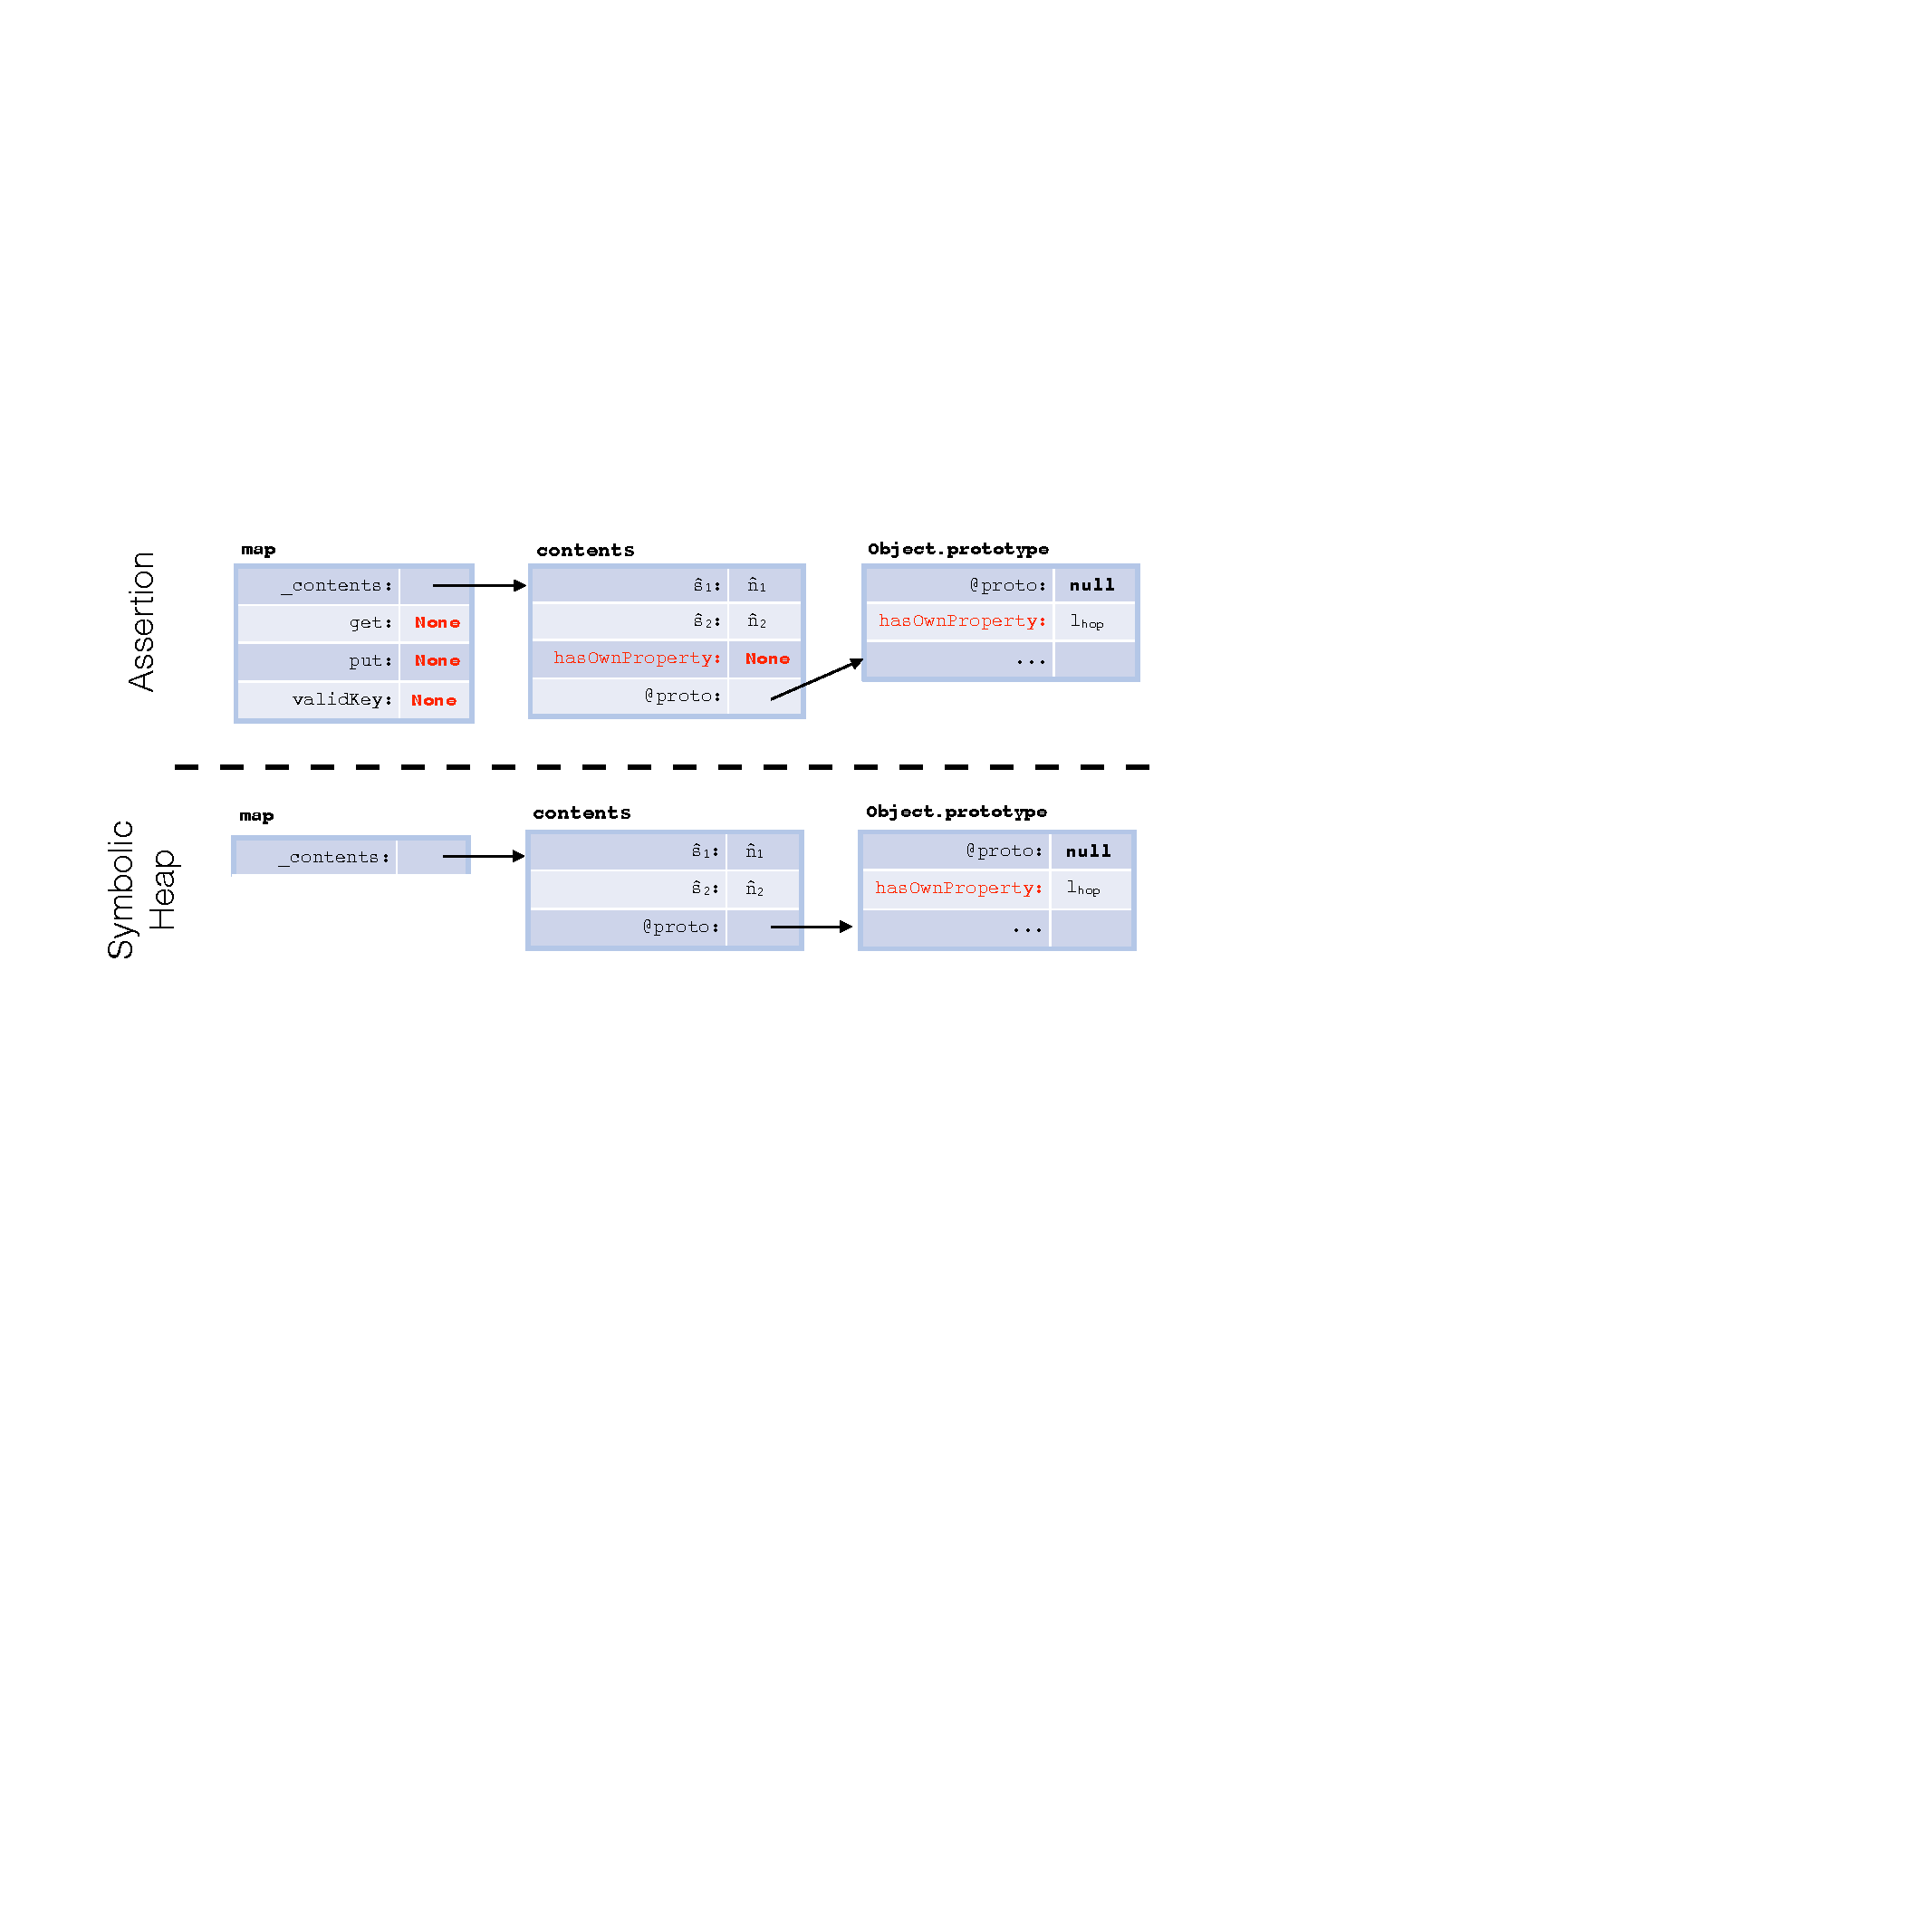
\includegraphics[width=0.9\textwidth]{figures/symbolicvsass.pdf}
{\small $$
\text{\emph{None-Constraints: }} (\hat{s}_1 \neq \texttt{"hasOwnProperty"} \, \wedge \, \hat{s}_2 \neq \texttt{"hasOwnProperty"})
$$}
\vspace{-25pt}
\caption{Assertion vs. Symbolic Heap}
\end{figure}



%\begin{algorithm}
%\caption{Synthesising a symbolic test for: $\lconf{P} \, \fid(\jvec{x}) \,  \lconf{Q}$}\label{infer:specs:algo}
%\begin{algorithmic}[1]
%\State $(\existentials, \sfs, \pfs) := \normalise(P)$ 
%\State $\sheap_0, \pfs_0, \theta := \concretise{(\existentials, \sfs, \pfs)}{[ \ ]}$
%\State $\subst' := \subst\mid_{\domain(\subst) \backslash \existentials}$
%\State Return: 
%%\ForAll{$XXX$}
%%\If{$XXX$}
%  %\State $\{ P \} \, \pid() \, \{ Q \} = \ispecs(\pid, \_)$
%%\Else
%  %\State $P,Q :=$
%%\EndIf
%%\State $ := InferSpec, \ispecs', \pid, P) $
%%\ForAll{$(Q_f,,\flag) \in $}
%%\If{$Q_f \sep Q_M \vdash Q \sep \true$}
%  %\State $\ispecs' := \ispecs' \cup \{(\pid, \flag) \mapsto {P \sep _f \sep Q_M}{\pid(\jvec{\xivar})}{Q_f \sep Q_M}\}$
%%\EndIf
%%\EndFor
%%\EndFor
%\end{algorithmic}
%\end{algorithm}


\subsection{Generating Symbolic Tests from JavaScript} 
\label{specs:example}

\myparagraph{Example}
In Figure~\ref{fig:map:example}, we define a \emph{map object predicate}, \jsinline|Map|, 
using the auxiliary predicate \jsinline|KVPairs|, which captures the resource of the key-value pairs in the map, 
and the \jsinline|validKey(k)| predicate, which holds if and only if the 
JavaScript function \jsinline|ValidKey(k)| returns \jsinline|true|\footnote{We treat the $\mathtt{ValidKey}$ predicate as a black box.}.
%
Intuitively, the \jsinline|Map(m, mp, kvs, keys)| predicate captures the resource 
of a map object \jsinline|m| with prototype \jsinline|mp|, keys \jsinline|keys| (a set of strings),
and key-value pairs \jsinline|kvs| (a set of string pairs\footnote{We model pairs as lists with two elements and, for clarity, use the pair notation.}). 
Observe that the definition of \jsinline|Map| does not include the resource of a map prototype, as
it is shared between all map objects, and therefore needs to be factored out.  
%
We write \jsinline|-u-| for set union and omit the brackets around singleton 
sets when the meaning is clear. % from the context. 

\begin{figure}[t!]
{\scriptsize
 \begin{verbatim}
Map (m, mp, kvs, keys) := JSObject(m, mp) * 
  DataProp(m, "_contents", c) * JSObject(c, Object.prototype) * KVPairs(c, kvs, keys) *
  (m, "get") -> None * (m, "put") ->  None * (m, "validKey") ->  None * 
  (c, "hasOwnProperty") ->  None *  emptyFields(c, keys -u- "hasOwnProperty")
  \end{verbatim}
  \vspace*{-0.3cm}
 \begin{verbatim}
KVPairs (o, kvs, keys) := 
  (kvs = { }) * (keys = { }),
  (kvs = (key, value) -u- kvs') * (keys = key -u- keys') * 
    ValidKey(key) * DataProp(o, key, value) * KVPairs(o, kvs', keys')
\end{verbatim}}
\caption{Map predicate \label{fig:map:example}}
\end{figure}

%In the following, we assume a \jsinline|MapProto| predicate specifying the resource of 
%a valid map prototype. In particular, the map prototype needs to define the methods 
%\jsinline|put|, \jsinline|get|, and \jsinline|validKey|. 


We are now in the position to specify the functions of the map library. In particular, below we show how to use 
the map object predicate to specify \jsinline|get(k)|.  
%
We consider the case in which the key whose value we  want to fetch is stored in the 
map.  The specification is given below. 
%
\begin{displaymath} 
{\footnotesize
\begin{array}{c}
\left\{ {\begin{array}{c}
 \text{\texttt{Map(this, mp, kvs -u- (k, v), ks) * ObjProtoF()}} \\ 
\end{array}} \right\} \\
%
\text{\bfseries \texttt{get(k)}} \\[0.2mm]
%
\left\{ {\begin{array}{c}
 \text{\texttt{Map(this, mp, kvs -u- (k, v), ks) * ObjProtoF() * (ret = v) }} \\
\end{array}} \right\}
\end{array}
} 
\end{displaymath}
%
The predicate \jsinline|ObjProtoF()| describes the resource captured by the \jsinline|Object.prototype| object. 
In particular, it is needed because \texttt{get} uses the \texttt{hasOwnProperty} function.



%%
%% OLD THINGS

%\begin{figure}[t!]
%\centering
%{\scriptsize
%\begin{mathpar} 
%\inferrule[\textsc{New Existential}]
%     { 
%         \svar \in \existentials 
%         \quad
%         \svar \not\in \domain(\subst)
%     }
%     {\unification{\sexpr, \pc}{\svar}{\subst}{\existentials} = \optionsome{\subst[\svar \mapsto \sexpr]}}
%\quad
%\inferrule[\textsc{Matched Existential}]
%     { 
%         \subst(\svar) = \sexpr' 
%         \quad 
%         \pc \vdash \sexpr = \sexpr' 
%     }
%     {\unification{\sexpr, \pc}{\svar}{\subst}{\existentials} = \optionsome{\subst}}
%\quad
%\inferrule[\textsc{Existential - None}]
%     { 
%         \subst(\svar) = \sexpr' 
%         \quad 
%         \pc \vdash \sexpr \neq \sexpr' 
%     }
%     {\unificationfail{\sexpr, \pc}{\svar}{\subst}{\existentials} = \optionnone}
%\\
%\inferrule[\textsc{Grounded Expression}]
%     { 
%         \fv(\subst(\sexpr')) \cap \existentials = \emptyset
%         \quad 
%          \pc \vdash  \sexpr = \subst(\sexpr') 
%     }
%     {\unification{\sexpr, \pc}{\sexpr'}{\subst}{\existentials} = \optionsome{\subst}}
%\qquad
%\inferrule[\textsc{Grounded Expression - Fail}]
%     { 
%         \fv(\subst(\sexpr')) \cap \existentials = \emptyset
%         \quad 
%          \pc  \vdash  \sexpr \neq \subst(\sexpr') 
%     }
%     {\unification{\sexpr, \pc}{\sexpr'}{\subst}{\existentials} = \optionnone}
%%
%\\
%\inferrule[\textsc{Cell Assertion}]
%	{  
%	   \big(\loc = \symbeval{\lexpr_l}{\sstore} \ \vee \loc = \subst(\symbeval{\lexpr_l}{\sstore}) \big)
%	   \quad 
%	     \symbeval{\lexpr_p}{\sstore} = \sexprp'
%	   \quad
%	   \symbeval{\lexpr_v}{\sstore} = \sexprv' 
%	   \quad
%	    \sheap = \sheap_f \dunion ((l, \sexprp) \mapsto \sexprv) 
%	   \\
%	   \unification{\sexprp, \pc}{\sexprp'}{\subst}{\existentials} = \optionsome{\subst'} 
%	   \quad
%	   \unification{\sexprv, \pc}{\sexprv'}{\subst'}{\existentials} = \optionsome{\subst''} 
%	}{ \unification{\sheap, \sstore, \pc}{(\lexpr_l,\lexpr_p)\pointsto \lexpr_v}{\subst}{\existentials} = \optionsome{(\subst'', \sheap_f)}} 
%\\
%\inferrule[\textsc{Cell Assertion - Fail}]
%	{  
%	   \big(\loc = \symbeval{\lexpr_l}{\sstore} \ \vee \loc = \subst(\symbeval{\lexpr_l}{\sstore}) \big)
%	   \quad
%	     \symbeval{\lexpr_p}{\sstore} = \sexprp'
%	   \quad
%	   \symbeval{\lexpr_v}{\sstore} = \sexprv' 
%	   \quad
%	     \sheap = \sheap' \dunion  \big((l, \sexprp_i) \mapsto \sexprv_i\big)\mid_{i = 0}^n   
%  	   \\
%	    (l, -) \not\in \domain(\sheap') 
%	    \quad 
%	   \forall_{0 \leq i \leq n} \, \unification{\sexprp, \pc}{\sexprp'}{\subst}{\existentials} = \optionnone 
%	   \ \vee \
%	   \unification{\sexprv, \pc}{\sexprv'}{\subst'}{\existentials} = \optionnone
%	}{ \unification{\sheap, \sstore, \pc}{(\lexpr_l,\lexpr_p)\pointsto \lexpr_v}{\subst}{\existentials} = \optionnone} 
%\\
%\inferrule[\textsc{EmptyFields Assertion}]
%	{  
%	   \big(\loc = \symbeval{\lexpr_l}{\sstore} \ \vee \loc = \subst(\symbeval{\lexpr_l}{\sstore}) \big)
%	   \quad 
%	     \symbeval{\lexpr_d}{\sstore} = \sexprv' 
%	   \\\\
%	     \sheap = \sheap' \, \uplus \, \big((l, \sexprp_i) \mapsto \sexprv_i\big)\mid_{i = 0}^n   
%              \quad
%             (l, -) \not\in \domain(\sheap')
%	    \quad 
%	    \pc \vdash \big( \{ \sexprp_i \mid_{i = 0}^n   \} \subseteq \sexprv' \big)
%	}{ \unification{\sheap, \sstore, \pc}{\emptyfields{\lexpr_l}{\lexpr_d}}{\subst}{\existentials} = \optionsome{(\subst, \sheap)}} 
%\\
%\inferrule[\textsc{EmptyFields Assertion - Failing}]
%	{  
%	   \big(\loc = \symbeval{\lexpr_l}{\sstore} \ \vee \loc = \subst(\symbeval{\lexpr_l}{\sstore}) \big)
%	   \quad 
%	     \symbeval{\lexpr_d}{\sstore} = \sexprv' 
%	   \\\\
%	     \sheap = \sheap' \, \uplus \, \big((l, \sexprp_i) \mapsto \sexprv_i\big)\mid_{i = 0}^n   
%              \quad
%             (l, -) \not\in \domain(\sheap')
%	    \quad 
%	    \pc \vdash \big( \{ \sexprp_i \mid_{i = 0}^n   \} \not\subseteq \sexprv' \big)
%	}{ \unification{\sheap, \sstore, \pc}{\emptyfields{\lexpr_l}{\lexpr_d}}{\subst}{\existentials} = \optionnone} 
%\end{mathpar}
%\hrule
%\caption{Unification of spatial assertions:
% {\scriptsize$\unification{\sheap, \sstore, \pc}{\cell}{\subst}{\existentials} = (\subst', \sheap_f)$}\label{fig:unification}}}
%\end{figure}


%{\small 
%\begin{align}
%\sepmodels{P} = \left\{ (\iheap, \store) \mid \exists \senv \, . \,  \iheap, \store, \senv \satisfies P  \right\} 
%\\ 
%\smodels{\isheap, \sstore}{\pc} = \left\{ (\iheap, \store) \mid \exists \senv \, . \,  \senv \vdash \pc \ \wedge \
%    \iheap = \symbeval{\isheap}{\senv} \ \wedge \ \store = \symbeval{\sstore}{\senv}  \right\} 
%\end{align}} 



%
%\begin{figure}
%{\scriptsize
%\centering
%\begin{mathpar} 
%\inferrule[\textsc{Spatial Assertion}]
%	{  
%	   \unification{\sheap, \sstore, \pc}{(\lexpr_l,\lexpr_p)\pointsto \lexpr_v}{\subst} = \uyes{\sheap_f}
%	}{\cellunification{\sheap, \cell \lstcons \cells}{\sheap_q, \cells}{\sstore, \pc, \subst}} 
%\\
%\inferrule[\textsc{Successful Unification}]
%	{  
%	   
%	   \cellunificationiter{\sheap, \cells}{\hemp, []}{\sstore, \pc, \subst}
%	   \qquad 
%	   \pc \vdash \subst(\pfs')
%%	   \cells =  \cell \lstcons \cells'
%%	   \and
%%            \unification{\sheap, \sstore, \pc}{\cell}{\subst} = \uyes{\sheap_f}
%%            \\\\
%%            \unificationfull{\sheap_f, \sstore, \pc}{\cells', \pfs'}{\subst}
%	}{\unificationfull{\sheap, \sstore, \pc}{\cells, \pfs'}{\subst}} 
%\and 
%\inferrule[\textsc{Spatial Assertion}]
%	{  
%	   \cells = \cell \lstcons \cells'
%	   \and
%            \unification{\sheap, \sstore, \pc}{\cell}{\subst} = \uyes{\sheap_f}
%            \\\\
%            \unificationfullfail{\sheap_f, \sstore, \pc}{\cells', \pfs'}{\subst}{\pc'}
%	}{\unificationfullfail{\sheap, \sstore, \pc}{\cells, \pfs'}{\subst}{\pc'}} 
%\\
%\inferrule[\textsc{Pure Assertions}]
%	{  
%	   \pc \vdash \subst(\pfs')
%	}{\unificationfull{\hemp, \sstore, \pc}{\emptyset, \pfs'}{\subst}} 
%%
%\and
%%
%\qquad
%\inferrule[\textsc{Pure Assertions -  Fail}]
%	{  
%	      \pc \not\vdash \subst(\pfs')
%	}{\unificationfullfail{\sheap, \sstore, \pc}{\emptyset, \pfs'}{\subst}{\subst(\pfs')}} 
%\\
%%
%\inferrule[\textsc{Cell Assertion - Fail}]
%	{  
%	   \sfs = \cells \lstcons \cells
%	   \and
%            \unification{\sheap, \sstore, \pc}{\cell}{\subst} = \uno{\pc'}
%	}{\unificationfullfail{\sheap, \sstore, \pc}{\sfs, \pfs'}{\subst}{\pc'}} 
%%
%\and
%\inferrule[\textsc{Extra Resource -  Fail}]
%	{  
%	    \sheap \neq \hemp
%	}{\unificationfullfail{\sheap, \sstore, \pc}{\emptyset, \pfs'}{\subst}{\jtrue}} 
%%
%\end{mathpar}}
%\hrule



%\newpage
%\section{From \jsil to JavaScript}\label{sec:lifting}
%


\section{Evaluation}\label{sec:evaluation}
%!TEX root = ../main.tex

We discuss the trustworthiness of \cosette and demonstrate that~our implementation, despite being  a proof-of-concept, has already proven useful for the debugging of real-world JavaScript code.
We elaborate on the results presented below in more detail in the Appendix. 

\myparagraph{Trustworthiness: JavaScript Semantics}
To ensure that Cosette follows the semantics of JavaScript without any simplifications, we tested \JSComp and our instrumented \jsil interpreter implemented in Rosette using Test262, the JavaScript official test suite~\cite{test262}. 
Out of the 10469 tests for ES5 Strict, we have identified 8330 tests appropriate for our coverage, of which we pass 100\%.

\myparagraph{Trustworthiness: Symbolic Interpreter} To make certain that the symbolic \jsil interpreter obtained by the Rosette lifting of the implemented instrumented interpreter is consistent with the symbolic semantics of \S\ref{subsec:symb:semantics}, we systematically constructed and successfully ran symbolic unit tests for each \jsil command, assuming the premises and asserting the conclusion of the appropriate rule of the symbolic semantics.

%With \cosette, we can write symbolic tests, in which some of the concrete values of the program are replaced with symbolic values.
%Symbolic tests improve on concrete tests for two main reasons.
%First, they are by construction more comprehensive than concrete tests, because symbolic tests can account for the whole range of values that a variable can take, instead of focusing on a few specific examples.
%Second, when \cosette finds a failing assertion inside a symbolic test, it can concretize the symbolic values into a counter-model that the developer can actually run in node, making debugging much easier compared to (the other things that we mention before).

\myparagraph{Whole-program Symbolic Testing: JS-Specific Features}
We created a number of symbolic tests to demonstrate that Cosette can reason about essential JavaScript features, such as prototype inheritance, function closures, arrays, strings, as well as the substantially more challenging for-in statement and dynamic dispatch. 

\myparagraph{Whole-program Symbolic Testing: Real-World Libraries}
We used \cosette to analyse the code of two JavaScript data structure libraries: Buckets.js~\cite{buckets}, and queue-pri~\cite{priq}.
We chose these libraries because reasoning about data structure code requires a precise description of the control flow features of JavaScript, because they come equipped with unit test suites, and because they do not have external dependencies (\cosette is a whole-program analysis); Buckets.js has over 65k downloads on npm.

For these two libraries, we wrote symbolic tests with the aim of obtaining a line coverage of 100\%, in order to compare them with the concrete unit tests that ship with the libraries.
In both cases, we were able to reduce the length of the tests by up to an average factor of 3, while increasing line coverage from around 90\% to a full 100\%.
We also discovered one bug in the Buckets.js library, as well as one in the queue-pri library.


The results are presented in table~\ref{cosette:res}.
For each file in the library, we report the number of JS executable lines in the code itself and including dependencies (slash-separated), the corresponding numbers of JSIL lines, the number of symbolic and concrete test cases, the number of JS lines in the symbolic and concrete tests, the coverage measured as percentage of lines and the average \cosette run time for the symbolic tests.
The files in Buckets.js are separated by a line from the unique file in queue-pri.

For the testing, we used a machine with an Intel Core i7-4980HQ CPU 2.80 GHz and DDR3 RAM 16GB. We measured the execution time of each symbolic test and averaged the times across tests for each library file. The times that we obtained reflect the fact that Rosette code is interpreted, rather than being run natively. We aim at implementing our own symbolic execution tool from scratch in the future, which, given our experience with JaVerT, should reduce execution times by at least an order of magnitude.

\begin{table}[!t]
{
\small
%\begin{center}
\setlength\tabcolsep{4pt}
\begin{tabular*}{\linewidth}{l@{\;\;}rrrrrr}
\toprule
% Name || JS Loc/loc* || JSIL Loc/loc* || #tests || symb/conc loc || symb/conc cov || time
Name & \makecell{JS lines} & \makecell{JSIL lines} & \# Tests & \makecell{Test lines} & \makecell{Line\\Cov.~(\%)} & \makecell{Avg.\\time} \\
\midrule
\texttt{arrays} & 44/71 & 1251/1942 & 9/24 & 166/329 & 100/100 & 20s \\
\texttt{bag} & 69/237 & 2041/7194 & 7/18 & 78/265 & 100/76.8 & 74s \\
\texttt{bstree} & 143/326 & 3819/8052 & 11/31 & 216/759 & 100/98.6 & 5m27s \\
\texttt{dict} & 57/84 & 1683/2374 & 7/14 & 116/170 & 100/80.7 & 15s \\
\texttt{heap} & 57/128 & 2059/4001 & 4/15 & 92/626 & 100/96.5 & 5m29s \\
\texttt{llist} & 126/153 & 2447/3138 & 9/21 & 149/370 & 100/94.4 & 24s \\
\texttt{multidict} & 56/184 & 1871/5496 & 6/16 & 118/189 & 100/74.1 & 1m15s \\
\texttt{pqueue} & 26/154 & 1066/5067 & 5/12 & 70/283 & 100/96.2 & 5m49s \\
\texttt{queue} & 30/183 & 1095/4233 & 6/9 & 111/146 & 100/96.7 & 20s \\
\texttt{set} & 40/124 & 1528/3902 & 6/12 & 86/271 & 100/70.0 & 1m01s \\
\texttt{stack} & 23/176 & 941/4079 & 4/7 & 91/104 & 100/87.0 & 26s \\
\midrule 
\texttt{queue-pri} & 19/164 & 872/5086 & 2/9 & 26/80 & 100/100 & xy.z \\
\bottomrule
%\end{center}
\end{tabular*}
}
\caption{Tests for the Buckets.js and queue-pri libraries}
\vspace*{-0.95cm}
\label{cosette:res}
\end{table}

%\pmax{Say something about how bugs work - sometimes coverage, sometimes semantics.}

\smallskip
\noindent \emph{Bug: MultiDictionary in Buckets.js.}
We have discovered a bug in the implementation of the Buckets.js multi-dictionary library.
A multi-dictionary is a key-value map in which a single key holds an array of distinct values. 
Our symbolic tests for the \jsinline|remove(key, value)| function, which removes a given key-value pair from the multi-dictionary, have revealed that the library wrongly treats the case in which we try to remove a key-value pair for a key with no associated values.
Concretely, a runtime error is thrown instead of \jsinline|remove| returning \jsinline|false|. 
This bug was not detected by the concrete unit tests associated with the library due to their incomplete coverage;
we have fixed it and submitted an appropriate pull request.




\smallskip
\noindent \emph{Bug: queue-pri.} This library implements a priority queue that stores data with an optional priority value.
The priority can either be a number (the lower the value, the higher the priority) or the default \jsinline{null} value if no priority is provided, in which case the associated element is put at the end of the queue. Our symbolic tests of the \jsinline{enqueue(data, pri)} method of the library have shown that that elements enqueued with priority \jsinline{0} were wrongly being always enqueued at the end of the queue. We traced the bug to the way in which priority was calculated inside \jsinline{enqueue}: \jsinline{priority = pri || null}, which evaluates to \jsinline|null| if the priority is not supplied, but also, due to the semantics of JavaScript, if it is equal to 0. This bug was not caught by the unit tests of the library because the developer had not considered inserting nodes with priority 0. This shows that \cosette is a useful tool for symbolic testing, because it fully follows the semantics of JavaScript and will expose corner cases that a developer may not be aware of.

\myparagraph{Specification-directed Bug-finding} 

\pmax{JaVerT examples - testing the unfolding, introducing bugs}

\section{Related Work}
\label{sec:rwc} 

The existing literature covers a wide range of JavaScript analysis techniques, including: 
type systems~\cite{thiemann:esop:2005,anderson:ecoop:2005,jensen:sas:2009,typescript:toot:2014,feldthaus:oopsla:2014,bierman:ecoop:2014,rastogi:popl:2015},
control flow analysis~\cite{feldthaus2013efficient}, pointer analysis~\cite{jang2009points,sridharan:ecoop:12} and abstract
interpretation~\cite{kashyap:fse:14,jensen:sas:2009,andreasen:oopsla:2014,park:ecoop:15}, among others. We focus on the existing work on symbolic execution and  
logic-based verification for JavaScript, and discuss general techniques for specification-driven 
test generation.  

\myparagraph{Symbolic Execution for JS}
The majority of the existing bug-finding symbolic execution tools for JavaScript target specific bug patterns, 
such as security vulnerabilities related to the misuse of strings~\cite{saxena:sp:2010} 
(for example, absence of sanitisation before security critical operations), malformed Web API requests~\cite{wittern:icse:2018}, and
DOM API specific bugs~\cite{li:fse:2014}. These tools are fully automatic and aim at code in 
the large, primarily focusing on scalability and coverage issues. \cosette has a different 
purpose: it is not designed to be fully automatic, but to \emph{assist} developers in 
testing their code. 
%
The work closest to ours is \emph{Jalangi}~\cite{koushik:fse:2015}, a general-purpose 
symbolic execution tool for JavaScript that implements a sophisticated state merging 
algorithm to deal with the problem of symbolic state explosion. 
%
However, Jalangi, as all existing symbolic execution tools for JavaScript, does not follow 
the semantics of the language precisely. 
%
In contrast, \cosette is \emph{trustworthy}: it does follow the semantics of 
JavaScript and its theoretical underpinnings are formalised and proven sound. 
Therefore, it can be used both as a basis for building other more specific analyses 
(e.g., combining symbolic execution with a type-based analysis to increase the precision of the latter) and 
as a testing oracle for other symbolic execution tools for JavaScript that purposely 
ignore some corner cases of the JavaScript semantics. 
Furthermore, \cosette is the first symbolic execution tool for JavaScript that provides 
frame resilience guarantees, which are essential for any specification-related reasoning.
%None of them can be used to test JS specs. 
%None offer insights into implementation either.

%
%\begin{itemize}
%   %\item \cite{saxena:sp:2010} - Kudzu
%  % \item \cite{li:fse:2014} - Toshiba guys
%   \item \polish{\cite{koushik:fse:2015} - jalangi} Jalangi~\cite{koushik:fse:2015} is the closest 
%            to ours in spirit. It is a general analysis. It does not model the JavaScript semantics 
%            precisely. 
%   %\item \cite{wittern:icse:2018} -  Julian 
%\end{itemize}

% \cite{saxena:sp:2010,li:fse:2014,koushik:fse:2015,wittern:icse:2018}


%\begin{itemize}
%   \item \cite{dolby:fse:2007} - Julian 
%   \item \cite{milicevic:icse:2007} \cite{boyapati:issta:2002} - Korat
%   \item \cite{seidel:esop:2015} - Target
%   \item \cite{claessen:icfp:2000} - QuickCheck. but also: FLOPS 2014 - Generating constrained random data with uniform distribution
%\end{itemize}

\myparagraph{Specification-driven Testing}
There is a long line of work on specification-driven test synthesis, dating back to 
\emph{Quickcheck}~\cite{claessen:icfp:2000}. \emph{Quickcheck} and its followers~\cite{runciman:haskell:2008,claessen:jfunc:2015}
translate Haskell type declarations into comprehensive test-suites. 
Recently, Seidel et al.~\cite{seidel:esop:2015} proposed \emph{Target}, a test generation tool 
that advances the agenda of \emph{Quickcheck} by supporting precise refinement types. 
The key insight of \emph{Target} is to use %combine the approach of \emph{Quickcheck} with the use of
an SMT solver for finding models for the supported type refinements. 
Specification-driven test generation has also been successfully applied to Java.
\emph{Korat}~\cite{boyapati:issta:2002,milicevic:icse:2007} generates test cases for Java classes annotated with
JML specifications~\cite{jml}, but it requires the class code to include 
a special Java method for checking if the class invariants hold. 
More recently, Dolby et al. \cite{dolby:fse:2007} proposed a SAT-based approach
for testing Java code annotated with relational logic specifications.
 %
To the best of our knowledge, there are no tools for specification-driven
testing of JavaScript, as well as no tools for test generation 
based on separation logic specifications.
 % 
 %With \cosette, one could easily concretise the resulting symbolic tests, effectively  obtaining a concrete test generation tool for JaVerT specifications.
 %
% However, the resulting tests would necessarily have a smaller coverage than the original symbolic tests; hence, we opted not to do this. 

\myparagraph{Logic-based Verification for JavaScript}
\javert~\cite{javert} is a verification toolchain for JavaScript based on separation logic. 
It comes with a trusted compiler, \JSComp, which we extend with constructs for creating and reasoning about symbolic values and reuse as part of \cosette. Like \cosette, \javert also performs its analysis on compiled \jsil code. However, the separation logic proof rules of \javert are not syntax-directed and offer little implementation insight; our novel symbolic semantics for \jsil is syntax-directed and is specifically designed to guide  implementations. JaVerT has been used to verify functional correctness properties of simple data structure libraries. We reuse the specifications of these libraries to evaluate our symbolic test generation mechanism.  
 
%There is little work on logic-based analyses for JavaScript.
%\citet{gardner:popl:2012} have developed JS Logic, a separation logic for a tiny fragment of ES3, to reason about the variable store emulated in the JavaScript heap. 
%This logic has proven difficult to automate and is not extensible to the entire language. 

Alternatively, we could have considered using the matching logic specifications of KJS~\cite{stefanescu:oopsla:2016}, a symbolic verification tool for core ES5 obtained by instantiating the general $\mathbb{K}$ framework with the semantics of JavaScript~\cite{Park:2015}. Similarly to \javert, KJS has been used to verify functional correctness properties of small data structure libraries.
However, KJS specifications are difficult to write and error-prone, as the developer has to  explicitly address all language internals. They are also not fully compositional, as they do not allow partial descriptions of JavaScript objects. 

There is also the work of \citet{swamy:pldi:2013}, who prove absence of runtime errors for higher-order JavaScript (ES3) programs by: compiling JS programs annotated with assertions and loop invariants to the logic of F*; generating verification conditions for the absence of runtime errors; and automatically discharging these conditions using Z3. However, as this analysis does not consider specifications, it was not possible for us to reuse its results for \cosette. 

All of the above-mentioned verification tools provide strong correctness guarantees, but have severe scalability limitations, as they require loop invariants and abstractions for the recursive structures that the programs use. In fact, none of these tools have been applied to real-world code. For instance, the Buckets.js library would be out of their reach, as they do not come with abstractions to accurately describe, for instance, JavaScript arrays, for-in loop invariants, and higher-order functions.  As a bug-finding tool, Cosette does not require any such abstractions, and can therefore be used for analysing substantially larger, more complex codebases.
% but the price paid is it can provide only bounded correctness guarantees when a bug has not been~found.


\section{Conclusions}

We have presented \cosette, a trustworthy, compositional symbolic execution
framework for JavaScript, combining the JS-2-JSIL compiler
and our JSIL symbolic interpreter written in Rosette. We
have applied Cosette to whole-program symbolic testing of real-world
JavaScript libraries and compositional debugging of separation logic
specifications of JavaScript programs.

We have developed a methodology for designing compositional program
analyses for dynamic languages in general, and symbolic execution for
JSIL in particular. We achieved this by introducing a new, abstract
semantics for JSIL, which we instantiated to obtain the concrete,
instrumented, and symbolic semantics. 
This abstract semantics is the bedrock for both the theoretical results 
and the implementation of the analysis. We prove that the \jsil symbolic 
execution of Cosette is
sound, frame-resilient and does not generate false positives. We
establish additional trust by using the theory to precisely guide the
implementation and by thorough~testing.

\cosette brings ideas from current separation logic research to the well-established 
setting of classical symbolic execution~\cite{andreasen:acmsurv:2017}. We believe that 
it is a stepping stone towards a {\em fully automatic} compositional symbolic execution 
tool for JavaScript in the style of Infer~\cite{calcagno:nasa:2011}. In future, 
our goal is to implement such a tool, using the \jsil abstract semantics presented here.


%\myparagraph{Entailment in Separation Logic and Countermodels}
%\begin{itemize}
%   \item 
%\end{itemize}



%
%\cite{gardner:popl:2012} have developed a separation logic for a small fragment of ECMAScript 3, to reason about the variable store emulated in the JavaScript heap.
%%
%\cite{rosu-serbanuta-2010-jlap} have developed $\mathbb{K}$, a term-rewriting framework  for  formalising the operational
%semantics of programming languages.
% In particular, they have developed KJS~\cite{Park:2015} which provides a $\mathbb{K}$-interpretation of the core language and part of the built-in libraries of the ES5 standard. KJS has been tested against the official ECMAScript Test262 test suite and passed all 2782 tests for the core language; the testing results for the built-in libraries are not reported. 
%\cite{stefanescu-park-yuwen-li-rosu-2016-oopsla} introduce a language-independent verification infrastructure 
%that can be instantiated with a $\mathbb{K}$-interpretation of a  language to automatically generate a symbolic verification tool for that language based on the $\mathbb{K}$ reachability logic. They apply this infrastructure to KJS to generate a verification tool for JavaScript, which they use to verify functional correctness properties of operations for manipulating data structures such as binary search trees, AVL trees, and lists.


%\section{Conclusions}\label{conclusions}

%\pmaxinline{Can we be more general, and say something like 'logic-based specifications'? It's all about translating to FOL, or even some version of PL. Also, we need to say at some point why we care about specifications written in separation logic.}

\newpage
\bibliographystyle{ACM-Reference-Format}
\bibliography{ppdp18}



\appendix

%!TEX root = ../main.tex

\newtheorem{lemmax}{}
\newtheorem{temax}{}

\section{\jsil Syntax and Semantics}


\begin{figure}[ht!]
{\scriptsize
\begin{mathpar} 
%
\inferrule[\textsc{Skip}]{}
	{ \semtrans{\heap, \store, \jsilskip}{\heap, \store}} 
 \qquad
 %
\inferrule[\textsc{Assignment}]
  {
      \symbeval{\jsilexpr}{\store} =  \val
      \quad
      \store' = \store[\jvar \mapsto \val]
  }{\semtrans{\heap, \store, \jvar := \jsilexpr}{\heap, \store'}} 
%
\qquad 
%
\inferrule[\textsc{Object Creation}]
  { 
    \heap = \heap \dunion \hcell{\loc}{\protop}{\jsnull}
    \quad (\loc,-) \notin \domain (\heap)
  }{\semtrans{\heap, \store, \jvar := \jsilnew()}{\heap, \store[\jvar \mapsto \loc]}}
\\
%
\inferrule[\textsc{Property Access}]
  { 
 	\symbeval{\jsilexpr_1}{\store} =  \loc
  	\quad 
        \symbeval{\jsilexpr_2}{\store} =  \jstring
        \quad
        \heap = - \dunion \hcell{\loc}{\jstring}{\val}
  }{ \semtrans{\heap, \store, \jvar := [\jsilexpr_1, \jsilexpr_2]}{\heap,  \store[\jvar \mapsto \val]}}
 \and 
 \inferrule[\textsc{Property Deletion}]
  { 
        \symbeval{\jsilexpr_1}{\store} =  \loc
  	\quad 
        \symbeval{\jsilexpr_2}{\store} =  \jstring
        \quad
        \heap = \heap' \dunion \hcell{\loc}{\jstring}{-}
  }{\semtrans{\heap, \store, \jsildelete(\jsilexpr_1, \jsilexpr_2)}{\heap', \store}}
 %
\\
%
\inferrule[\textsc{Property Assignment - Found}]
  {     \symbeval{\jsilexpr_1}{\store} =  \loc
  	\quad 
        \symbeval{\jsilexpr_2}{\store} =  \jstring
        \quad
        \symbeval{\jsilexpr_3}{\store} =  \val
       \\\\
        \heap = \heap' \dunion  \hcell{\loc}{\jstring}{-}
  }{\semtrans{\heap, \store, [\jsilexpr_1, \jsilexpr_2] := \jsilexpr_3}{\heap' \dunion  \hcell{\loc}{\jstring}{\val}, \store}} 
 \and 
 \inferrule[\textsc{Property Assignment - Not Found}]
  {     \symbeval{\jsilexpr_1}{\store} =  \loc
  	\quad 
        \symbeval{\jsilexpr_2}{\store} =  \jstring
        \quad
        \symbeval{\jsilexpr_3}{\store} =  \val
       \\\\
        \heap = \heap' 
        \quad 
        (\loc, \jstring) \not\in \domain(\heap)
  }{\semtrans{\heap, \store, [\jsilexpr_1, \jsilexpr_2] := \jsilexpr_3}{\heap \dunion  \hcell{\loc}{\jstring}{\val}, \store}} 
\\
%
\inferrule[\textsc{Member Check - True}]
  { 
      \symbeval{\jsilexpr_1}{\store} =  \loc
  	\quad 
        \symbeval{\jsilexpr_2}{\store} =  \jstring
       \quad 
   	(\loc, \jstring) \in \domain(\heap) 
  }{\semtrans{\heap, \store,\jvar := \hasfield(\jsilexpr_1, \jsilexpr_2)}{\heap, \store[\jvar \mapsto \jtrue]}}
  \and 
 \inferrule[\textsc{Member Check - False}]
  { 
      \symbeval{\jsilexpr_1}{\store} =  \loc
  	\quad 
        \symbeval{\jsilexpr_2}{\store} =  \jstring
       \quad 
   	(\loc, \jstring) \not\in \domain(\heap) 
  }{\semtrans{\heap, \store,\jvar := \hasfield(\jsilexpr_1, \jsilexpr_2)}{\heap, \store[\jvar \mapsto \jfalse]}}
%
\\
%
\inferrule[\textsc{Assert - True}]
  { 
      \symbeval{\jsilexpr}{\store} =  \jtrue
  }{\semtrans{\heap, \store, \assert(\jsilexpr)}{\heap, \store}} 
\and
\inferrule[\textsc{Assert - False}]
  { 
      \symbeval{\jsilexpr}{\store} \neq \jtrue
  }{\semtranserr{\heap, \store, \assert(\jsilexpr)}} 
\end{mathpar}}
\caption{Symbolic Execution for Basic Commands: {\scriptsize$\semtrans{\heap, \store, \bcmd}{\heap', \store'}$}\label{fig:sem:basic:commands}}
\end{figure}




\begin{figure}[ht!]
{\scriptsize
\begin{mathpar} 
\inferrule[\textsc{Basic Command}]
   { 
     \prog_{\pid}(i) = \bcmd 
     \quad
     \semtrans{\heap, \store, \bcmd}{\heap', \store'} 
   }{\semtrans{\heap, \store, \ctx[i]}{\heap', \store', \ctx[i+1]}}
%
   \qquad
  %
  \inferrule[\textsc{Basic Command - Fail}]
   { 
     \prog_{\pid}(i) = \bcmd 
     \quad
     \semtranserr{\heap, \store, \bcmd} 
   }{\semtranserr{\heap, \store, \ctx[i]}}
 %
   \qquad
  %
  \inferrule[\textsc{Goto}]
   { \prog_{\pid}(i) = \goto \, j \quad}
   {\semtrans{\heap, \store, \ctx[i]}{\heap, \store, \ctx[j]}}
  \\ 
  \inferrule[\textsc{Cond. Goto - True}]
   { \prog_{\pid}(i) =  \ifgoto{\jsilexpr}{j}{k} \quad
     \symbeval{\jsilexpr}{\store} =  \jtrue
   }
   {\semtrans{\heap, \store, \ctx[i]}{\heap, \store, \ctx[j]}}
  \and 
    \inferrule[\textsc{Cond. Goto - False}]
   { \prog_{\pid}(i) =  \ifgoto{\jsilexpr}{j}{k} \quad
     \symbeval{\jsilexpr}{\store} =  \jfalse
   }
   {\semtrans{\heap, \store, \ctx[i]}{\heap, \store, \ctx[k]}}
   \\
    \inferrule[\textsc{Procedure Call}]
   { 
    \prog_{\pid}(i) =   \jsilcall{\jvar}{\jsilexpr}{\jsilexpr_i \mid_{i = 0}^{n}}{j}
     \quad
    \symbeval{\jsilexpr}{\sstore} =  \pid' 
        \quad
     \args(\pid') = \jsillist{\jvar_1, ..., \jvar_{m}} 
      \quad
      \val_i = \symbeval{\jsilexpr_i}{\sstore} \mid_{i = 0}^{n} 
     \ 
      \val_i = \jsundefined \mid_{i = n+1}^{m}  
   }
   {\semtrans{\heap, \store, \ctx[i]}{\heap, [ \jvar_i \mapsto \val_i \mid_{i = 0}^{m}] , ((\pid', \store, \jvar, i+1, j)::\ctx)[0]}}
    \\ 
  \inferrule[\textsc{Normal Return}]
   {
       \ctx = (-, \store', \jvar, i, -) :: \ctx' 
       \quad 
       \store(\procretvar) = \val
   }  
   {\semtrans{\heap, \store, \ctx[\procretlab]}{\heap, \store'[\jvar \mapsto \val], \ctx'[i]}}
   \and 
     \inferrule[\textsc{Error Return}]
   {
       \ctx = (-, \store', \jvar, -, j) :: \sctx' 
       \quad 
       \sstore(\procerrvar) = \val
   }
   {\semtrans{\heap, \store, \ctx[\procerrlab]}{\sheap, \store'[\jvar \mapsto \val], \ctx'[j]}}
 \end{mathpar}}
\caption{Symbolic Execution for Control Flow Commands: {\scriptsize$\semtrans{\heap, \store, \ctx[i]}{\heap', \store', \ctx'[j]}$}} 
\end{figure}


\begin{figure}[ht!]
{\scriptsize
\begin{mathpar} 
\inferrule[\textsc{Basic Command}]
   { 
     \ccmd[\prog][\ctx]{i} = \bcmd 
     \quad
     \semtrans{\heap, \store, \bcmd}{\heap', \store'} 
   }{\semtrans[\prog]{\heap, \store, i}{\heap', \store', i+1}[C]}
%
   \qquad
  %
  \inferrule[\textsc{Basic Command - Fail}]
   { 
     \ccmd[\prog][\ctx]{i} = \bcmd 
     \quad
     \semtranserr{\heap, \store, \bcmd} 
   }{\semtranserr[\prog]{\heap, \store, i}[C]}
 %
   \qquad
  %
  \inferrule[\textsc{Goto}]
   { \ccmd[\prog][\ctx]{i} = \goto \, j \quad}
   {\semtrans[\prog]{\heap, \store, i}{\heap, \store, j}[C]}
  \\ 
  \inferrule[\textsc{Cond. Goto - True}]
   { \ccmd[\prog][\ctx]{i} =  \ifgoto{\jsilexpr}{j}{k} \quad
     \symbeval{\jsilexpr}{\store} =  \jtrue
   }
   {\semtrans[\prog]{\heap, \store, i}{\heap, \store, j}[C]}
  \and 
    \inferrule[\textsc{Cond. Goto - False}]
   { \ccmd[\prog][\ctx]{i} =  \ifgoto{\jsilexpr}{j}{k} \quad
     \symbeval{\jsilexpr}{\store} =  \jfalse
   }
   {\semtrans[\prog]{\heap, \store, i}{\heap, \store, k}[C]}
   \\
    \inferrule[\textsc{Procedure Call}]
   { 
    \ccmd[\prog][\ctx]{i} =   \jsilcall{\jvar}{\jsilexpr}{\jsilexpr_i \mid_{i = 0}^{n}}{j}
     \quad
    \symbeval{\jsilexpr}{\sstore} =  \pid' 
        \quad
     \args(\pid') = \jsillist{\jvar_1, ..., \jvar_{m}} 
      \quad
      \val_i = \symbeval{\jsilexpr_i}{\sstore} \mid_{i = 0}^{n} 
     \ 
      \val_i = \jsundefined \mid_{i = n+1}^{m}  
   }
   {\semtrans[\prog]{\heap, \store, i}{\heap, [ \jvar_i \mapsto \val_i \mid_{i = 0}^{m}] , 0}[C][(\pid', \store, \jvar, i+1, j) :: \ctx]}
    \\ 
  \inferrule[\textsc{Normal Return}]
   {
       \ctx = (-, \store', \jvar, i, -) :: \ctx' 
       \quad 
       \store(\procretvar) = \val
   }  
   {\semtrans[\prog]{\heap, \store, \procretlab}{\heap, \store'[\jvar \mapsto \val], i}[C][C']}
   \and 
     \inferrule[\textsc{Error Return}]
   {
       \ctx = (-, \store', \jvar, -, j) :: \ctx' 
       \quad 
       \store(\procerrvar) = \val
   }
   {\semtrans[\prog]{\heap, \store, \procerrlab}{\heap, \store'[\jvar \mapsto \val], j}[C][C']}
 \end{mathpar}}
 \pmax{What happens when we exit from main, how do we stop? Basically, cmd, returns nothing and we can't reduce?}
 \vspace*{-0.4cm}
\caption{Symbolic Execution for Control Flow Commands: $\semtrans[\prog]{\heap, \store, i}{\heap', \store', j}[C][C']$}
\end{figure}

\begin{figure}[ht!]
{\scriptsize
\begin{mathpar} 
\inferrule[\textsc{Basic Command}]
   { 
     \ccmd{i} = \bcmd 
     \quad
     \semtrans{\heap, \store, \bcmd}{\heap', \store'} 
   }{\semtrans{\heap, \store, i}{\heap', \store', i+1}}
%
   \qquad
  %
  \inferrule[\textsc{Basic Command - Fail}]
   { 
     \ccmd{i} = \bcmd 
     \quad
     \semtranserr{\heap, \store, \bcmd} 
   }{\semtranserr{\heap, \store, i}}
 %
   \qquad
  %
  \inferrule[\textsc{Goto}]
   { \ccmd{i} = \goto \, j \quad}
   {\semtrans{\heap, \store, i}{\heap, \store, j}}
  \\ 
  \inferrule[\textsc{Cond. Goto - True}]
   { \ccmd{i} =  \ifgoto{\jsilexpr}{j}{k} \quad
     \symbeval{\jsilexpr}{\store} =  \jtrue
   }
   {\semtrans{\heap, \store, i}{\heap, \store, j}}
  \and 
    \inferrule[\textsc{Cond. Goto - False}]
   { \ccmd{i} =  \ifgoto{\jsilexpr}{j}{k} \quad
     \symbeval{\jsilexpr}{\store} =  \jfalse
   }
   {\semtrans{\heap, \store, i}{\heap, \store, k}}
   \\
    \inferrule[\textsc{Procedure Call}]
   { 
    \ccmd{i} = \jsilcall{\jvar}{\jsilexpr}{\jsilexpr_i \mid_{i = 0}^{n}}{j}
     \quad
    \symbeval{\jsilexpr}{\sstore} =  \pid' 
        \quad
     \args(\pid') = \jsillist{\jvar_1, ..., \jvar_{m}} 
      \quad
      \val_i = \symbeval{\jsilexpr_i}{\sstore} \mid_{i = 0}^{n} 
     \ 
      \val_i = \jsundefined \mid_{i = n+1}^{m}  
   }
   {\semtrans{\heap, \store, i}{\heap, [ \jvar_i \mapsto \val_i \mid_{i = 0}^{m}] , 0}[C][(\pid', \store, \jvar, i+1, j) :: \ctx]}
    \\ 
  \inferrule[\textsc{Normal Return}]
   {
       \ctx = (-, \store', \jvar, i, -) :: \ctx' 
       \quad 
       \store(\procretvar) = \val
   }  
   {\semtrans{\heap, \store, \procretlab}{\heap, \store'[\jvar \mapsto \val], i}[C][C']}
   \and 
     \inferrule[\textsc{Error Return}]
   {
       \ctx = (-, \store', \jvar, -, j) :: \ctx' 
       \quad 
       \store(\procerrvar) = \val
   }
   {\semtrans{\heap, \store, \procerrlab}{\heap, \store'[\jvar \mapsto \val], j}[C][C']}
 \end{mathpar}}
 \vspace*{-0.4cm}
\caption{Symbolic Execution for Control Flow Commands: $\semtrans[\prog]{\heap, \store, i}{\heap', \store', j}[C][C']$}
\end{figure}

\section{Proofs - Section~\ref{sec:jsil:symb:exec}}

\begin{lemma}[Soundess of symbolic execution for \jsil basic commands]\label{soundness:basic:commands}
$$
\begin{array}{l}
\symbtrans{\sheap, \sstore, \bcmd, \pc}{\sheap', \sstore', \pc'}
   \ \wedge \ 
      (\heap, \store) \in \smodels{\sheap, \sstore}{\pc'} \\ \quad \quad
      	 \ \implies \ \exists (\heap', \store') \, . \, 
	 	 \semtrans{\heap, \store, \bcmd}{\heap', \store'}
		\, \wedge \, 
		(\heap', \store') \in \smodels{\sheap', \sstore'}{\pc'}  
\end{array}
$$
\end{lemma}
\begin{proof}
We proceed by case analysis on $\symbtrans{\sheap, \sstore, \bcmd, \pc}{\sheap', \sstore', \pc'}$. 
\vspace{5pt}

\noindent\prooflab{Skip} 
We conclude that $\bcmd = \jsilskip$, and 
that $\sheap' = \sheap$, $\sstore' = \sstore$, and $\pc' = \pc$. 
By picking $\heap' = \heap$, $\store' = \store$, the result follows. 
\vspace{6pt}

\noindent\prooflab{Assignment} 
We conclude that $\bcmd = \jvar := \jsilexpr$, for some variable $\jvar$ and expression $\jsilexpr$, 
and that $\sheap' = \sheap$, $\sstore' = \sstore[\jvar \mapsto \symbeval{\jsilexpr}{\store}]$, and $\pc' = \pc$. 
From $(\heap, \store) \in \smodels{\sheap, \sstore}{\pc'}$, we conclude that there is a symbolic environment 
$\senv$ such that $\heap = \semexpr{\sheap}{\senv}$ and $\store = \semexpr{\sstore}{\senv}$. 
Noting that: 
$$
 \semtrans{\heap, \store, \jvar := \jsilexpr}{\heap, \store[\jvar \mapsto \symbeval{\jsilexpr}{\store}]}
% \qquad 
 %\semexpr{\sstore[\jvar \mapsto \symbeval{\jsilexpr}{\store}]}{\senv} = \semexpr{\sstore}{\senv}[\jvar \mapsto \symbeval{\jsilexpr}{\store, \senv}]
$$
we pick $\heap' = \heap$ and $\store' =  \store[\jvar \mapsto \symbeval{\jsilexpr}{\store}]$. We 
now have to prove that $(\heap', \store') \in \smodels{\sheap', \sstore'}{\pc}$.
Observing that: 
$$
\heap' =  \semexpr{\sheap}{\senv} = \semexpr{\sheap'}{\senv} 
\quad 
\store' = \semexpr{\sstore}{\senv}[\jvar \mapsto \symbeval{\jsilexpr}{\semexpr{\sstore}{\senv}}]
   = \semexpr{\sstore[\jvar \mapsto \symbeval{\jsilexpr}{\store}]}{\senv} 
   = \semexpr{\sstore'}{\senv}
$$
%
the result follows. 
\vspace{6pt}

\noindent\prooflab{Object Creation}
We conclude that $\bcmd = \jvar := \jsilnew()$, for some variable $\jvar$, and that
$\sheap' = \sheap \dunion \hcell{\loc}{\protop}{\jsnull}$, $\sstore' = \sstore[\jvar \mapsto \loc]$, and $\pc' = \pc$, 
 where  $(\loc,-) \notin \domain (\sheap)$. 
 From $(\heap, \store) \in \smodels{\sheap, \sstore}{\pc'}$, we conclude that there is a symbolic environment
$\senv$ such that $\heap = \semexpr{\sheap}{\senv}$ and $\store = \semexpr{\sstore}{\senv}$. 
Noting that: 
$$
\semtrans{\heap, \store, \jvar := \jsilnew()}{\heap \dunion \hcell{\loc}{\protop}{\jsnull}, \store[\jvar \mapsto \loc]}
$$
where: $(\loc,-) \notin \domain (\heap)$, we pick $\heap' = \semexpr{\sheap}{\senv} \dunion \hcell{\loc}{\protop}{\jsnull}$ 
and $\store' = \semexpr{\sstore}{\senv}[\jvar \mapsto \loc]$. 
We now have to prove that $(\heap', \store') \in \smodels{\sheap', \sstore'}{\pc}$.
Noting that: 
$$
\begin{array}{l}
\heap' = \semexpr{\sheap}{\senv} \dunion \hcell{\loc}{\protop}{\jsnull} = \semexpr{\sheap \dunion \hcell{\loc}{\protop}{\jsnull}}{\senv}   
     = \semexpr{\sheap'}{\senv}  \\
%
\store' = \semexpr{\sstore}{\senv}[\jvar \mapsto \loc] = \semexpr{\sstore}{\senv}[\jvar \mapsto \symbeval{\loc}{\senv}] = 
      \semexpr{\sstore[\jvar \mapsto \loc]}{\senv} = \semexpr{\sstore'}{\senv} 
\end{array}
$$
the result follows. 
\vspace{6pt}

\noindent\prooflab{Property Access}
We conclude that $\bcmd = \jvar := [\jsilexpr_1, \jsilexpr_2]$, for some variable $\jvar$, and expressions $\jsilexpr_1$ and $\jsilexpr_2$, 
and that $\sheap' = \sheap$, $\sstore' = \sstore[\jvar \mapsto \sexprv_k]$, and: 
 $$\pc' =  \pc \ \wedge \, \big( (\sexprp_k = \sexpr_p) \ \wedge \bigwedge_{i = 0, i \neq k}^n (\sexprp_i \neq \sexpr_p) \big)$$
 where 
 $\symbeval{\jsilexpr_1}{\sstore} =  \loc$, $\symbeval{\jsilexpr_2}{\sstore} =  \sexpr_p$, 
 $\sheap = \sheap'' \, \uplus \, \big((l, \sexprp_i) \mapsto \sexprv_i\big)\mid_{i = 0}^n$, 
 $(l, -) \not\in \domain(\sheap')$, and $0 \leq k \leq n$. 
%
From $(\heap, \store) \in \smodels{\sheap, \sstore}{\pc'}$, we conclude that there is a symbolic environment
$\senv$ such that $\heap = \semexpr{\sheap}{\senv}$, $\store = \semexpr{\sstore}{\senv}$, and 
$\senv \vdash \pc'$. 
We now have to prove that we can apply the \prooflab{Property Access} rule in the concrete state.
To this end, we have to show that there is a concrete heap $\heap''$ such that:
$\heap = \heap'' \dunion \hcell{\symbeval{\jsilexpr_1}{\store}}{\symbeval{\jsilexpr_2}{\store}}{\symbeval{\jsilexpr_3}{\store}}$. 
Note that: 
$$
\begin{array}{l}
%
 \symbeval{\jsilexpr_1}{\store} = \symbeval{\jsilexpr_1}{\symbeval{\sstore}{\senv}} = \symbeval{\symbeval{\jsilexpr_1}{\sstore}}{\senv} 
    = \symbeval{\loc}{\senv} = \loc \\ 
 %
  \symbeval{\jsilexpr_2}{\store}  = \symbeval{\jsilexpr_2}{\semexpr{\sstore}{\senv}} =  \symbeval{\symbeval{\jsilexpr_2}{\sstore}}{\senv}
   =  \symbeval{\sexpr_p}{\senv} = \symbeval{\sexprp_k}{\senv}  \text{ (because $\senv \vdash \pc'$ and $\pc' \vdash \sexprp_k = \sexpr_p$)} \\
 %
 \heap = \semexpr{\sheap'' \, \uplus \, \big((l, \sexprp_i) \mapsto \sexprv_i\big)\mid_{i = 0}^n}{\senv} 
       =  \semexpr{\sheap'' \, \uplus \, \big((l, \sexprp_i) \mapsto \sexprv_i\big)\mid_{i = 0, i \neq k}^n}{\senv} \dunion \semexpr{(l, \sexprp_k) \mapsto \sexprv_k}{\senv} \\
         \qquad = \semexpr{\sheap'' \, \uplus \, \big((l, \sexprp_i) \mapsto \sexprv_i\big)\mid_{i = 0, i \neq k}^n}{\senv} \dunion (l, \semexpr{\sexprp_k}{\senv}) \mapsto \semexpr{\sexprv_k}{\senv}  \\ 
         \qquad =  \semexpr{\sheap'' \, \uplus \, \big((l, \sexprp_i) \mapsto \sexprv_i\big)\mid_{i = 0, i \neq k}^n}{\senv} \dunion (\symbeval{\jsilexpr_1}{\store}, \symbeval{\jsilexpr_2}{\store}) \mapsto \semexpr{\sexprv_k}{\senv}
\end{array}
$$
We can now apply the \prooflab{Property Access} rule of \jsil semantics, concluding: 
$$
   \semtrans{\heap, \store, \jvar := [\jsilexpr_1, \jsilexpr_2]}{\heap,  \store[\jvar \mapsto \semexpr{\sexprv_k}{\senv}]}
$$
meaning that: $\heap' = \heap$ and $\store' = \store[\jvar \mapsto \semexpr{\sexprv_k}{\senv}]$.
We have now to prove that $(\heap', \store') \in \smodels{\sheap', \sstore'}{\pc'}$.
Observe that: 
$$
\begin{array}{l}
\heap' = \heap = \semexpr{\sheap}{\senv}   = \semexpr{\sheap'}{\senv}  \text{ (because $\heap' = \heap$ and $ \sheap = \sheap'$)}
\\
 \store' =  \semexpr{\sstore}{\senv}[\jvar \mapsto \symbeval{\sexprv_k}{\senv}] 
    =  \semexpr{\sstore[\jvar \mapsto \sexprv_k]}{\senv} 
    =  \semexpr{\sstore'}{\senv}
\end{array}
$$
 which concludes the proof. 
\vspace{6pt}

\noindent\prooflab{Property Deletion}
We conclude that $\bcmd = \jsildelete(\jsilexpr_1, \jsilexpr_2)$, for some expressions $\jsilexpr_1$ and $\jsilexpr_2$
and that: 
$$
\begin{array}{l}
\sheap' = \sheap'' \, \uplus \,  \big((\loc, \sexprp_i) \mapsto \sexprv_i\big)\mid_{i = 0, i \neq k}^n
\quad 
\sstore' = \sstore
\\ 
 \pc' = \pc \ \wedge \, \big( (\sexprp_k = \sexpr_p) \ \wedge \bigwedge_{i = 0, i \neq k}^n (\sexprp_i \neq \sexpr_p) \big)
\end{array}
$$
where $\loc = \symbeval{\jsilexpr_1}{\sstore}$ and $\sexpr_p = \symbeval{\jsilexpr_2}{\sstore}$
From $(\heap, \store) \in \smodels{\sheap, \sstore}{\pc'}$, we conclude that there is a symbolic environment
$\senv$ such that $\heap = \semexpr{\sheap}{\senv}$, $\store = \semexpr{\sstore}{\senv}$, and 
$\senv \vdash \pc'$. 
We now have to prove that we can apply the \prooflab{Property Deletion} rule in the concrete state.
To this end, we have to show that:
$\heap = \heap' \dunion \hcell{\symbeval{\jsilexpr_1}{\store}}{\symbeval{\jsilexpr_2}{\store}}{-}$. 
Note that: 
$$
\begin{array}{l}
%
 \symbeval{\jsilexpr_1}{\store} = \symbeval{\jsilexpr_1}{\symbeval{\sstore}{\senv}} = \symbeval{\symbeval{\jsilexpr_1}{\sstore}}{\senv} 
    = \symbeval{\loc}{\senv} = \loc \\ 
 %
  \symbeval{\jsilexpr_2}{\store}  = \symbeval{\jsilexpr_2}{\semexpr{\sstore}{\senv}} =  \symbeval{\symbeval{\jsilexpr_2}{\sstore}}{\senv}
   =  \symbeval{\sexpr_p}{\senv} = \symbeval{\sexprp_k}{\senv}  \text{ (because $\senv \vdash \pc'$ and $\pc' \vdash \sexprp_k = \sexpr_p$)} \\
 %
 \heap = \semexpr{\sheap'' \, \uplus \, \big((l, \sexprp_i) \mapsto \sexprv_i\big)\mid_{i = 0}^n}{\senv} 
       =  \semexpr{\sheap'' \, \uplus \, \big((l, \sexprp_i) \mapsto \sexprv_i\big)\mid_{i = 0, i \neq k}^n}{\senv} \dunion \semexpr{(l, \sexprp_k) \mapsto \sexprv_k}{\senv} \\
         \qquad = \semexpr{\sheap'' \, \uplus \, \big((l, \sexprp_i) \mapsto \sexprv_i\big)\mid_{i = 0, i \neq k}^n}{\senv} \dunion (l, \semexpr{\sexprp_k}{\senv}) \mapsto \semexpr{\sexprv_k}{\senv}  \\ 
         \qquad =  \semexpr{\sheap'' \, \uplus \, \big((l, \sexprp_i) \mapsto \sexprv_i\big)\mid_{i = 0, i \neq k}^n}{\senv} \dunion (\symbeval{\jsilexpr_1}{\store}, \symbeval{\jsilexpr_2}{\store}) \mapsto \semexpr{\sexprv_k}{\senv} \\ 
         \qquad = \semexpr{\sheap'}{\senv} \dunion (\symbeval{\jsilexpr_1}{\store}, \symbeval{\jsilexpr_2}{\store}) \mapsto -
\end{array}
$$
We can now apply the \prooflab{Property Deletion} rule of \jsil semantics, concluding: 
$$
   \semtrans{\heap, \store, \jsildelete(\jsilexpr_1, \jsilexpr_2)}{\semexpr{\sheap'}{\senv},  \store}
$$
meaning that: $\heap' = \semexpr{\sheap'}{\senv}$ and $\store' = \store$.
We have now to prove that $(\heap', \store') \in \smodels{\sheap', \sstore'}{\pc'}$.
Noting that $\heap' = \semexpr{\sheap'}{\senv}$ and $\store' = \store = \semexpr{\sstore}{\senv} = \semexpr{\sstore'}{\senv}$, 
the result follows. 
\vspace{6pt}

\noindent\prooflab{Property Assignment - Found}
We conclude that  $\bcmd = [\jsilexpr_1, \jsilexpr_2] := \jsilexpr_3$ for some expressions $\jsilexpr_1$, $\jsilexpr_2$, 
and $\jsilexpr_3$, and that: 
$$
\begin{array}{l}
  \sheap =  \sheap'' \, \uplus \, \big((l, \sexprp_i) \mapsto \sexprv_i\big)\mid_{i = 0}^n    \\
  %
  \sheap' = \sheap'' \, \uplus \,  \big((l, \sexprp_i) \mapsto \sexprv_i\big)\mid_{i = 0, i \neq k}^n \, \uplus \,  (l, \sexpr_p) \mapsto \sexpr_v  \\
  %
  \sstore' = \sstore \\ 
  %
  \pc' = \pc \ \wedge \, \big( (\sexprp_k = \sexpr_p) \ \wedge \bigwedge_{i = 0, i \neq k}^n (\sexprp_i \neq \sexpr_p)
\end{array}
$$ 
where $\symbeval{\jsilexpr_1}{\sstore} =  \loc$, $\symbeval{\jsilexpr_2}{\sstore} =  \sexpr_p$, 
$\symbeval{\jsilexpr_3}{\sstore} =  \sexpr_v$.
From $(\heap, \store) \in \smodels{\sheap, \sstore}{\pc'}$, we conclude that there is a symbolic environment
$\senv$ such that $\heap = \semexpr{\sheap}{\senv}$, $\store = \semexpr{\sstore}{\senv}$, and 
$\senv \vdash \pc'$. 
We now have to prove that we can apply the \prooflab{Property Assignment - Found} rule in the concrete state.
To this end, we have to show that there is a concrete heap $\heap''$ such that:
$\heap = \heap'' \dunion \hcell{\symbeval{\jsilexpr_1}{\store}}{\symbeval{\jsilexpr_2}{\store}}{-}$. 
Note that: 
$$
\begin{array}{l}
%
 \symbeval{\jsilexpr_1}{\store} = \symbeval{\jsilexpr_1}{\symbeval{\sstore}{\senv}} = \symbeval{\symbeval{\jsilexpr_1}{\sstore}}{\senv} 
    = \symbeval{\loc}{\senv} = \loc \\ 
 %
  \symbeval{\jsilexpr_2}{\store}  = \symbeval{\jsilexpr_2}{\semexpr{\sstore}{\senv}} =  \symbeval{\symbeval{\jsilexpr_2}{\sstore}}{\senv}
   =  \symbeval{\sexpr_p}{\senv} = \symbeval{\sexprp_k}{\senv}  \text{ (because $\senv \vdash \pc'$ and $\pc' \vdash \sexprp_k = \sexpr_p$)} \\
 %
  \symbeval{\jsilexpr_3}{\store}  = \symbeval{\jsilexpr_3}{\semexpr{\sstore}{\senv}} =  \symbeval{\symbeval{\jsilexpr_3}{\sstore}}{\senv}
   =  \symbeval{\sexpr_v}{\senv} \\
 %
 \heap = \semexpr{\sheap'' \, \uplus \, \big((l, \sexprp_i) \mapsto \sexprv_i\big)\mid_{i = 0}^n}{\senv} 
       =  \semexpr{\sheap'' \, \uplus \, \big((l, \sexprp_i) \mapsto \sexprv_i\big)\mid_{i = 0, i \neq k}^n}{\senv} \dunion \semexpr{(l, \sexprp_k) \mapsto \sexprv_k}{\senv} \\
         \qquad = \semexpr{\sheap'' \, \uplus \, \big((l, \sexprp_i) \mapsto \sexprv_i\big)\mid_{i = 0, i \neq k}^n}{\senv} \dunion (l, \semexpr{\sexprp_k}{\senv}) \mapsto \semexpr{\sexprv_k}{\senv}  \\ 
         \qquad =  \semexpr{\sheap'' \, \uplus \, \big((l, \sexprp_i) \mapsto \sexprv_i\big)\mid_{i = 0, i \neq k}^n}{\senv} \dunion (\symbeval{\jsilexpr_1}{\store}, \symbeval{\jsilexpr_2}{\store}) \mapsto \semexpr{\sexprv_k}{\senv} \\ 
\end{array}
$$
We can now apply the \prooflab{Property Assignment - Found} rule of \jsil semantics, concluding: 
$$
   \semtrans{\heap, \store, [\jsilexpr_1, \jsilexpr_2] := \jsilexpr_3}
     {\semexpr{\sheap'' \, \uplus \, \big((l, \sexprp_i) \mapsto \sexprv_i\big)\mid_{i = 0, i \neq k}^n}{\senv} \dunion (\symbeval{\jsilexpr_1}{\store}, \symbeval{\jsilexpr_2}{\store}) \mapsto \symbeval{\jsilexpr_3}{\store},  \store}
$$
meaning that: 
$\heap' = \symbeval{\sheap'' \, \uplus \, \big((l, \sexprp_i) \mapsto \sexprv_i\big)\mid_{i = 0, i \neq k}^n}{\senv} \dunion (\symbeval{\jsilexpr_1}{\store}, \symbeval{\jsilexpr_2}{\store}) \mapsto \symbeval{\jsilexpr_3}{\store}$ and 
$\store' = \store$.
We have now to prove that $(\heap', \store') \in \smodels{\sheap', \sstore'}{\pc'}$.
Noting that:
$$
\begin{array}{l}
\heap' = \symbeval{\sheap'' \, \uplus \, \big((l, \sexprp_i) \mapsto \sexprv_i\big)\mid_{i = 0, i \neq k}^n}{\senv} \dunion (\symbeval{\jsilexpr_1}{\store}, \symbeval{\jsilexpr_2}{\store}) \mapsto \symbeval{\jsilexpr_3}{\store} \\ 
  \qquad = \symbeval{\sheap'' \, \uplus \, \big((l, \sexprp_i) \mapsto \sexprv_i\big)\mid_{i = 0, i \neq k}^n}{\senv} \dunion (\loc, \symbeval{\sexpr_p}{\senv}) \mapsto \symbeval{\sexpr_v}{\senv}  \\
    \qquad = \symbeval{\sheap'' \, \uplus \, \big((l, \sexprp_i) \mapsto \sexprv_i\big)\mid_{i = 0, i \neq k}^n \dunion (\loc, \sexpr_p) \mapsto \sexpr_v}{\senv}  \\
    \qquad = \symbeval{\sheap'}{\senv} \\[2pt]
 %
 \store' = \store = \symbeval{\sstore}{\senv} = \symbeval{\sstore'}{\senv} 
\end{array}
$$
the result follows. 
\vspace{6pt}

\noindent\prooflab{Property Assignment - Not Found}
We conclude that  $\bcmd = [\jsilexpr_1, \jsilexpr_2] := \jsilexpr_3$ for some expressions $\jsilexpr_1$, $\jsilexpr_2$, 
and $\jsilexpr_3$, and that: 
$$
\begin{array}{l}
  \sheap =   \sheap'' \, \uplus \, \big((l, \sexprp_i) \mapsto \sexprv_i\big)\mid_{i = 0}^n     \\
  %
  \sheap' =  \sheap \, \uplus \,  (l, \sexpr_p) \mapsto \sexpr_v  \\
  %
  \sstore' = \sstore \\ 
  %
    \pc' = \pc \ \wedge \, \bigwedge_{i = 0}^n (\sexprp_i \neq \sexpr_p)
\end{array}
$$ 
where $\symbeval{\jsilexpr_1}{\sstore} =  \loc$, $\symbeval{\jsilexpr_2}{\sstore} =  \sexpr_p$, 
$\symbeval{\jsilexpr_3}{\sstore} =  \sexpr_v$,  $(\loc, -) \not\in \domain(\sheap'')$, 
and $0 \leq k \leq n$. 
From $(\heap, \store) \in \smodels{\sheap, \sstore}{\pc'}$, we conclude that there is a symbolic environment
$\senv$ such that $\heap = \semexpr{\sheap}{\senv}$, $\store = \semexpr{\sstore}{\senv}$, and 
$\senv \vdash \pc'$. 
We have now to prove that we can apply the \prooflab{Property Assignment - Found} rule in the concrete state.
To this end, we have to show that:
$(\symbeval{\jsilexpr_1}{\store}, \symbeval{\jsilexpr_2}{\store}) \not\in \domain(\heap)$. 
Note that: 
$$
\begin{array}{l}
%
 \symbeval{\jsilexpr_1}{\store} = \symbeval{\jsilexpr_1}{\symbeval{\sstore}{\senv}} = \symbeval{\symbeval{\jsilexpr_1}{\sstore}}{\senv} 
    = \symbeval{\loc}{\senv} = \loc \\ 
 %
  \symbeval{\jsilexpr_2}{\store}  = \symbeval{\jsilexpr_2}{\semexpr{\sstore}{\senv}} =  \symbeval{\symbeval{\jsilexpr_2}{\sstore}}{\senv}
   =  \symbeval{\sexpr_p}{\senv} \\
 %
  \symbeval{\jsilexpr_3}{\store}  = \symbeval{\jsilexpr_3}{\semexpr{\sstore}{\senv}} =  \symbeval{\symbeval{\jsilexpr_3}{\sstore}}{\senv}
   =  \symbeval{\sexpr_v}{\senv} \\
 %
 \heap = \semexpr{\sheap'' \, \uplus \, \big((l, \sexprp_i) \mapsto \sexprv_i\big)\mid_{i = 0}^n}{\senv} \\
    \qquad = \semexpr{\sheap''}{\senv} \dunion \biguplus_{0 \leq i \leq n} ((l, \symbeval{\sexprp_i}{\senv}) \mapsto \symbeval{\sexprv_i}{\senv})
\end{array}
$$
From  $(\loc, -) \not\in \domain(\sheap'')$, we conclude that $(\loc, -) \not\in \domain(\semexpr{\sheap''}{\senv})$. 
Since $\senv \vdash \pc'$, we additionally conclude that: 
$
  \forall_{0 \leq i \leq n}  \, \symbeval{\sexprp_i}{\senv} \neq \symbeval{\sexpr_p}{\senv} 
$
Recalling that $\symbeval{\jsilexpr_2}{\store} = \symbeval{\sexpr_p}{\senv}$, we conclude that  
$
  \forall_{0 \leq i \leq n}  \, \symbeval{\sexprp_i}{\senv} \neq \symbeval{\jsilexpr_2}{\store}
$, from which it follows (together with $(\loc, -) \not\in \domain(\semexpr{\sheap''}{\senv})$) that 
$(\symbeval{\jsilexpr_1}{\store}, \symbeval{\jsilexpr_2}{\store}) \not\in \domain(\heap)$.
We can now apply the \prooflab{Property Assignment - Not Found} rule of \jsil semantics, concluding: 
$$
   \semtrans{\heap, \store, [\jsilexpr_1, \jsilexpr_2] := \jsilexpr_3}
     {\heap \dunion (\symbeval{\jsilexpr_1}{\store}, \symbeval{\jsilexpr_2}{\store}) \mapsto \symbeval{\jsilexpr_3}{\store},  \store}
$$
meaning that $\heap' = \heap \dunion (\symbeval{\jsilexpr_1}{\store}, \symbeval{\jsilexpr_2}{\store}) \mapsto \symbeval{\jsilexpr_3}{\store}$ 
and $\store' = \store$. 
%
We have now to prove that $(\heap', \store') \in \smodels{\sheap', \sstore'}{\pc'}$.
Noting that:
$$
\begin{array}{l}
\heap' = \symbeval{\sheap}{\senv} \dunion (\symbeval{\jsilexpr_1}{\store}, \symbeval{\jsilexpr_2}{\store}) \mapsto \symbeval{\jsilexpr_3}{\store} \\ 
  \qquad = \symbeval{\sheap}{\senv} \dunion (\loc, \symbeval{\sexpr_p}{\senv}) \mapsto \symbeval{\sexpr_v}{\senv}  \\
    \qquad = \symbeval{\sheap \dunion (\loc, \sexpr_p) \mapsto \sexpr_v}{\senv}  \\
    \qquad = \symbeval{\sheap'}{\senv} \\[2pt]
 %
 \store' = \store = \symbeval{\sstore}{\senv} = \symbeval{\sstore'}{\senv} 
\end{array}
$$
the result follows. 
\vspace{6pt}



\noindent\prooflab{Member Check - True}
We conclude that  $\bcmd = \jvar := \hasfield(\jsilexpr_1, \jsilexpr_2)$ for some variable $\jvar$ and expressions $\jsilexpr_1$ and $\jsilexpr_2$, and that: 
$$
\begin{array}{l}
  \sheap =   \sheap'' \, \uplus \, \big((l, \sexprp_i) \mapsto -\big)\mid_{i = 0}^n     \\
  %
  \sheap' =  \sheap \\
  %
  \sstore' = \sstore[\jvar \mapsto \jtrue] \\ 
  %
    \pc' = \pc \ \wedge \, \big( (\sexprp_k = \sexpr_p) \ \wedge \bigwedge_{i = 0, i \neq k}^n (\sexprp_i \neq \sexpr_p) \big)
\end{array}
$$ 
where $\symbeval{\jsilexpr_1}{\sstore} =  \loc$, $\symbeval{\jsilexpr_2}{\sstore} =  \sexpr_p$, 
$(\loc, -) \not\in \domain(\sheap'')$, and $0 \leq k \leq n$. 
%
From $(\heap, \store) \in \smodels{\sheap, \sstore}{\pc'}$, we conclude that there is a symbolic environment
$\senv$ such that $\heap = \semexpr{\sheap}{\senv}$, $\store = \semexpr{\sstore}{\senv}$, and 
$\senv \vdash \pc'$. 
We have now to prove that we can apply the \prooflab{Member Check - True} rule in the concrete state.
To this end, we have to show that:
$\heap = \heap'' \dunion (\symbeval{\jsilexpr_1}{\store}, \symbeval{\jsilexpr_2}{\store}) \mapsto -$, for 
some concrete heap $\heap''$. 
Note that: 
$$
\begin{array}{l}
%
 \symbeval{\jsilexpr_1}{\store} = \symbeval{\jsilexpr_1}{\symbeval{\sstore}{\senv}} = \symbeval{\symbeval{\jsilexpr_1}{\sstore}}{\senv} 
    = \symbeval{\loc}{\senv} = \loc \\ 
 %
  \symbeval{\jsilexpr_2}{\store}  = \symbeval{\jsilexpr_2}{\semexpr{\sstore}{\senv}} =  \symbeval{\symbeval{\jsilexpr_2}{\sstore}}{\senv}
   =  \symbeval{\sexpr_p}{\senv} \\
 %
 \heap = \semexpr{\sheap'' \, \uplus \, \big((l, \sexprp_i) \mapsto \sexprv_i\big)\mid_{i = 0}^n}{\senv} \\
    \qquad = \semexpr{\sheap'' \, \uplus \, \big((l, \sexprp_i) \mapsto \sexprv_i\big)\mid_{i = 0, i\neq k}^n \dunion (l, \sexprp_k) \mapsto \sexprv_k}{\senv} \\
    \qquad = \semexpr{\sheap'' \, \uplus \, \big((l, \sexprp_i) \mapsto \sexprv_i\big)\mid_{i = 0, i\neq k}^n}{\senv} \dunion \semexpr{(l, \sexprp_k) \mapsto \sexprv_k}{\senv} \\
    \qquad = \semexpr{\sheap'' \, \uplus \, \big((l, \sexprp_i) \mapsto \sexprv_i\big)\mid_{i = 0, i\neq k}^n}{\senv} \dunion (l, \semexpr{\sexprp_k}{\senv}) \mapsto \semexpr{\sexprv_k}{\senv} \\ 
     \qquad = \semexpr{\sheap'' \, \uplus \, \big((l, \sexprp_i) \mapsto \sexprv_i\big)\mid_{i = 0, i\neq k}^n}{\senv} \dunion (l, \semexpr{\sexpr_p}{\senv}) \mapsto \semexpr{\sexprv_k}{\senv}
      			\text{ (using $\senv \vdash \pc$)} \\ 
     \qquad = \semexpr{\sheap'' \, \uplus \, \big((l, \sexprp_i) \mapsto \sexprv_i\big)\mid_{i = 0, i\neq k}^n}{\senv} \dunion (\symbeval{\jsilexpr_1}{\store}, \symbeval{\jsilexpr_2}{\store}) \mapsto - \\
\end{array}
$$
We can now apply the \prooflab{Member Check - True} rule of \jsil semantics, concluding: 
$$
   \semtrans{\heap, \store, \jvar := \hasfield(\jsilexpr_1, \jsilexpr_2)}{\heap,  \store[\jvar \mapsto \jtrue]}
$$
meaning that $\heap' = \heap$ and $\store' = \store[\jvar \mapsto \jtrue]$. 
%
We have now to prove that $(\heap', \store') \in \smodels{\sheap', \sstore'}{\pc'}$.
Noting that:
$$
\begin{array}{l}
\heap' = \heap = \semexpr{\sheap}{\senv} = \semexpr{\sheap'}{\senv} \\
 %
 \store' = \store[\jvar \mapsto \jtrue] = \symbeval{\sstore}{\senv}[\jvar \mapsto \jtrue]  = \symbeval{\sstore[\jvar \mapsto \jtrue]}{\senv} = \symbeval{\sstore'}{\senv} 
\end{array}
$$
the result follows. 
\vspace{6pt}


\noindent\prooflab{Member Check - False}
We conclude that  $\bcmd = \jvar := \hasfield(\jsilexpr_1, \jsilexpr_2)$ for some variable $\jvar$ and expressions $\jsilexpr_1$ and $\jsilexpr_2$, and that: 
$$
\begin{array}{l}
  \sheap =  \sheap'' \, \uplus \, \big((l, \sexprp_i) \mapsto -\big)\mid_{i = 0}^n      \\
  %
  \sheap' =  \sheap \\
  %
  \sstore' = \sstore[\jvar \mapsto \jfalse] \\ 
  %
     \pc' = \pc \ \wedge \,  \bigwedge_{i = 0}^n (\sexprp_i \neq \sexpr_p) 
\end{array}
$$ 
where $\symbeval{\jsilexpr_1}{\sstore} =  \loc$, $\symbeval{\jsilexpr_2}{\sstore} =  \sexpr_p$, 
$(\loc, -) \not\in \domain(\sheap'')$, and $0 \leq k \leq n$. 
%
From $(\heap, \store) \in \smodels{\sheap, \sstore}{\pc'}$, we conclude that there is a symbolic environment
$\senv$ such that $\heap = \semexpr{\sheap}{\senv}$, $\store = \semexpr{\sstore}{\senv}$, and 
$\senv \vdash \pc'$. 
We have now to prove that we can apply the \prooflab{Member Check - False} rule in the concrete state.
To this end, we have to show that: $(\symbeval{\jsilexpr_1}{\store}, \symbeval{\jsilexpr_2}{\store}) \not\in \domain(\heap)$. 
Note that: 
$$
\begin{array}{l}
%
 \symbeval{\jsilexpr_1}{\store} = \symbeval{\jsilexpr_1}{\symbeval{\sstore}{\senv}} = \symbeval{\symbeval{\jsilexpr_1}{\sstore}}{\senv} 
    = \symbeval{\loc}{\senv} = \loc \\ 
 %
  \symbeval{\jsilexpr_2}{\store}  = \symbeval{\jsilexpr_2}{\semexpr{\sstore}{\senv}} =  \symbeval{\symbeval{\jsilexpr_2}{\sstore}}{\senv}
   =  \symbeval{\sexpr_p}{\senv} \\
 %
 \heap = \semexpr{\sheap'' \, \uplus \, \big((l, \sexprp_i) \mapsto \sexprv_i\big)\mid_{i = 0}^n}{\senv} \\
    \qquad = \semexpr{\sheap''}{\senv} \dunion \biguplus_{0 \leq i \leq n} (l, \semexpr{\sexprp_i}{\senv}) \mapsto \semexpr{\sexprv_i}{\senv}
\end{array}
$$
Since $(\loc, -) \not\in \domain(\sheap'')$, we conclude that $(\loc, -) \not\in \semexpr{\sheap''}{\senv}$. 
%
Since $\senv \vdash \pc'$, we additionally conclude that: 
$
  \forall_{0 \leq i \leq n}  \, \symbeval{\sexprp_i}{\senv} \neq \symbeval{\sexpr_p}{\senv} 
$
Recalling that $\symbeval{\jsilexpr_2}{\store} = \symbeval{\sexpr_p}{\senv}$, we conclude that  
$
  \forall_{0 \leq i \leq n}  \, \symbeval{\sexprp_i}{\senv} \neq \symbeval{\jsilexpr_2}{\store}
$, from which it follows (together with $(\loc, -) \not\in \domain(\semexpr{\sheap''}{\senv})$) that 
$(\symbeval{\jsilexpr_1}{\store}, \symbeval{\jsilexpr_2}{\store}) \not\in \domain(\heap)$.
%
We can now apply the \prooflab{Member Check - False} rule of \jsil semantics, concluding: 
$$
   \semtrans{\heap, \store, \jvar := \hasfield(\jsilexpr_1, \jsilexpr_2)}{\heap,  \store[\jvar \mapsto \jfalse]}
$$
meaning that $\heap' = \heap$ and $\store' = \store[\jvar \mapsto \jfalse]$. 
%
Now we have to prove that $(\heap', \store') \in \smodels{\sheap', \sstore'}{\pc'}$.
Noting that:
$$
\begin{array}{l}
\heap' = \heap = \semexpr{\sheap}{\senv} = \semexpr{\sheap'}{\senv} \\
 %
 \store' = \store[\jvar \mapsto \jfalse] = \symbeval{\sstore}{\senv}[\jvar \mapsto \jfalse]] = \symbeval{\sstore[\jvar \mapsto \jfalse]}{\senv} = \symbeval{\sstore'}{\senv} 
\end{array}
$$
the result follows. 
\vspace{6pt}


\noindent\prooflab{Assert - True}
We conclude that  $\bcmd = \assert(\jsilexpr)$ for some expression $\jsilexpr$, and that: 
$$
  \sheap' = \sheap 
  \quad
  \sstore' =  \sstore 
  \quad
  \pc' = \pc
  \quad
  \pc \vdash  \symbeval{\jsilexpr}{\sstore}
$$ 
From $(\heap, \store) \in \smodels{\sheap, \sstore}{\pc'}$, we conclude that there is a symbolic environment
$\senv$ such that $\heap = \semexpr{\sheap}{\senv}$, $\store = \semexpr{\sstore}{\senv}$, and 
$\senv \vdash \pc$. 
We have now to prove that we can apply the \prooflab{Assert - True} rule in the concrete state.
To this end, we have to show that: $\symbeval{\jsilexpr}{\store} = \jtrue$. 
Noting that:
$
  \symbeval{\jsilexpr}{\store} = \symbeval{\jsilexpr}{\symbeval{\sstore}{\senv}} 
         = \symbeval{\symbeval{\jsilexpr}{\sstore}}{\senv} 
$, we conclude (using $\senv \vdash \pc$ and $\pc \vdash  \symbeval{\jsilexpr}{\sstore}$) that 
$\symbeval{\jsilexpr}{\store} = \jtrue$. 
We can now apply the \prooflab{Assert - True} rule of \jsil semantics, concluding: 
$$
   \semtrans{\heap, \store, \assert(\jsilexpr)}{\heap,  \store}
$$
meaning that $\heap' = \heap$ and $\store' = \store$. 
%
Now we have to prove that $(\heap', \store') \in \smodels{\sheap', \sstore'}{\pc'}$.
Noting that:
$$
\begin{array}{l}
\heap' = \heap = \semexpr{\sheap}{\senv} = \semexpr{\sheap'}{\senv}
 %
 \quad 
 %
 \store' = \store = \symbeval{\sstore}{\senv} = \symbeval{\sstore}{\senv} = \symbeval{\sstore'}{\senv} 
\end{array}
$$
the result follows. 
\vspace{6pt}

\noindent\prooflab{Assert - False}
We conclude that  $\bcmd = \assert(\jsilexpr)$ for some expression $\jsilexpr$, and that: 
$\pc \not\vdash  \symbeval{\jsilexpr}{\sstore}$. 
From $(\heap, \store) \in \smodels{\sheap, \sstore}{\pc'}$, we conclude that there is a symbolic environment
$\senv$ such that $\heap = \semexpr{\sheap}{\senv}$, $\store = \semexpr{\sstore}{\senv}$, and 
$\senv \vdash \pc$. 
We have now to prove that we can apply the \prooflab{Assert - False} rule in the concrete state.
To this end, we have to show that: $\symbeval{\jsilexpr}{\store} = \jfalse$. 
Noting that:
$
  \symbeval{\jsilexpr}{\store} = \symbeval{\jsilexpr}{\symbeval{\sstore}{\senv}} 
         = \symbeval{\symbeval{\jsilexpr}{\sstore}}{\senv} 
$, we conclude (using $\senv \vdash \pc$ and $\pc \not\vdash  \symbeval{\jsilexpr}{\sstore}$) that 
$\symbeval{\jsilexpr}{\store} = \jfalse$, from which the result follows. 
\end{proof}


\begin{temax}[Theorem~\ref{teo:soundness:jsil:symb:exe} - Soundess of \jsil symbolic execution]
$$
\begin{array}{l}
\symbtrans{\sheap, \sstore, \sctx[i], \pc}{\sheap', \sstore', \sctx'[j], \pc'} 
   \ \wedge \ 
      (\heap, \store, \ctx) \in \smodels{\sheap, \sstore, \sctx}{\pc'} \\ \quad \quad
      	 \ \implies \ \exists (\heap', \store', \ctx') \, . \, 
	 	 \semtrans{\heap, \store, \ctx[i]}{\heap', \store', \ctx'[j]}
		\, \wedge \, 
		(\heap', \store', \ctx') \in \smodels{\sheap', \sstore', \sctx'}{\pc'}  
\end{array}
$$
\end{temax}
%
\begin{proof}
We proceed by case analysis on $\symbtrans{\sheap, \sstore, \sctx[i], \pc}{\sheap', \sstore', \sctx'[j], \pc'}$. 
\vspace{5pt}

\noindent\prooflab{Basic Command} 
We conclude that $\prog_{\pid}(i) = \bcmd$ for some basic command $\bcmd$,  
$\symbtrans{\sheap, \sstore, \bcmd, \pc}{\sheap', \sstore', \pc'}$, 
$\sctx' = \sctx$, and $j = i + 1$. 
Since $(\heap, \store, \ctx) \in \smodels{\sheap, \sstore, \sctx}{\pc'}$, we conclude 
that $(\heap, \store) \in \smodels{\sheap, \sstore}{\pc'}$. 
Applying Lemma~\ref{soundness:basic:commands} to: 
$$ 
\symbtrans{\sheap, \sstore, \bcmd, \pc}{\sheap', \sstore', \pc'} 
\qquad 
(\heap, \store) \in \smodels{\sheap, \sstore}{\pc'}
$$
we conclude that there is a concrete heap $\heap'$ and store $\store'$ such 
that: 
$$
\semtrans{\heap, \store, \bcmd}{\heap', \store'}
\qquad 
(\heap', \store') \in \smodels{\sheap', \sstore'}{\pc'}  
$$
Using $\prog_{\pid}(i) = \bcmd$ and $\semtrans{\heap, \store, \bcmd}{\heap', \store'}$, 
we can apply the \prooflab{Basic Command} rule of \jsil semantics to conclude 
that: $\semtrans{\heap, \store, \ctx[i]}{\heap', \store', \ctx[i+1]}$. 
From $\sctx' = \sctx$, $(\heap', \store') \in \smodels{\sheap', \sstore'}{\pc'}$, 
and $(\heap, \store, \ctx) \in \smodels{\sheap, \sstore, \sctx}{\pc'}$, it follows
that $(\heap', \store', \ctx') \in \smodels{\sheap, \sstore, \sctx}{\pc'}$, 
which concludes the proof. 
\vspace{6pt}


\noindent\prooflab{Goto} 
We conclude that $\prog_{\pid}(i) = \goto \, k$ for some program index $k$ and 
that $\symbtrans{\sheap, \sstore, \sctx[i], \pc}{\sheap, \sstore, \sctx[k], \pc}$, 
meaning that $\sheap' = \sheap$, $\sstore' = \sstore$, $\sctx' = \sctx$, $j = k$, 
and $\pc' = \pc$. 
From $\prog_{\pid}(i) = \goto \, k$, we conclude that 
$\semtrans{\heap, \store, \ctx[i]}{\heap, \store, \ctx[k]}$. 
Noting that: 
$$
(\heap', \store', \ctx') = (\heap, \store, \ctx) \in \smodels{\sheap, \sstore}{\pc}  = \smodels{\sheap', \sstore'}{\pc'}
$$
the result follows. 
\vspace{6pt}


\noindent\prooflab{Cond. Goto - True} 
We conclude that $\prog_{\pid}(i) = \ifgoto{\jsilexpr}{k_1}{k_2}$ for some expression 
$\jsilexpr$ and indexes $k_1$ and $k_2$ and 
that $\symbtrans{\sheap, \sstore, \sctx[i], \pc}{\sheap, \sstore, \sctx[k_1], \pc \, \wedge \, \sexpr}$, 
meaning that $\sheap' = \sheap$, $\sstore' = \sstore$, $\sctx' = \sctx$, $j = k$, 
and $\pc' = \pc \, \wedge \, \sexpr$, where $\semexpr{\jsilexpr}{\sstore} = \sexpr$. 
Since $(\heap, \store, \ctx) \in \smodels{\sheap, \sstore, \sctx}{\pc'}$, we conclude that 
there is a symbolic environment $\senv$ such that: $\senv \vdash \pc'$, 
$\heap = \semexpr{\sheap}{\senv}$, $\store = \semexpr{\sstore}{\senv}$, 
and $\ctx = \semexpr{\sctx}{\senv}$.
From  $\senv \vdash \pc' = \pc \ \wedge \ \sexpr$, it follows that $\symbeval{\sexpr}{\senv} = \jtrue$. 
Noting that: 
$$
\semexpr{\jsilexpr}{\store} = \semexpr{\jsilexpr}{\semexpr{\sstore}{\senv}} 
    = \semexpr{\semexpr{\jsilexpr}{\sstore}}{\senv} 
    = \semexpr{\sexpr}{\senv}
    = \jtrue
$$
we conclude that $\semtrans{\heap, \store, \ctx[i]}{\heap, \store, \ctx[k_1]}$. 
Noting that: 
$$
(\heap', \store', \ctx') = (\heap, \store, \ctx) \in \smodels{\sheap, \sstore}{\pc}  = \smodels{\sheap', \sstore'}{\pc'}
$$
the result follows. 
\vspace{6pt}


\noindent\prooflab{Procedure Call} 
We conclude that $\prog_{\pid}(i) =   \jsilcall{\jvar}{\jsilexpr}{\jsilexpr_i \mid_{i = 0}^{n}}{j}$
for some variable $\jvar$, expressions $\jsilexpr$, $\jsilexpr_0$, ..., $\jsilexpr_n$, and 
index $j$, and that:
$$
\sheap' = \sheap
%
\qquad
% 
\sstore' = [ \jvar_i \mapsto \val_i \mid_{i = 0}^{m}] 
%
\qquad 
%
\ctx' = ((\pid', \sstore, \jvar, i+1, j)::\sctx
%
\qquad
\pc' = \pc
$$
where $\pid' = \symbeval{\jsilexpr}{\sstore}$,  
$\jsillist{\jvar_1, ..., \jvar_{m}} = \args(\pid')$, and: 
$$
\sexpr_i = \left\lbrace{\begin{array}{ll}
\symbeval{\jsilexpr_i}{\sstore} & \text{if } 0 \leq i \leq n \\
\jsundefined                            & \text{otherwise}
\end{array}}\right.
$$
Since $(\heap, \store, \ctx) \in \smodels{\sheap, \sstore, \sctx}{\pc'}$, we conclude that 
there is a symbolic environment $\senv$ such that: $\senv \vdash \pc'$, 
$\heap = \semexpr{\sheap}{\senv}$, $\store = \semexpr{\sstore}{\senv}$, 
and $\ctx = \semexpr{\sctx}{\senv}$.
Noting that: 


%    \inferrule[\textsc{Procedure Call}]
%   { 
%    \prog_{\pid}(i) =   \jsilcall{\jvar}{\jsilexpr}{\jsilexpr_i \mid_{i = 0}^{n}}{j}
%     \quad
%    \symbeval{\jsilexpr}{\sstore} =  \pid' 
%    \quad
%      \symbeval{\jsilexpr_i}{\sstore} =  \sexpr_i \mid_{i = 0}^{n} 
%     \quad
%     \args(\pid') = \jsillist{\jvar_1, ..., \jvar_{m}} 
%     \quad 
%      \sexpr_i = \jsundefined \mid_{i = n+1}^{m}  
%   }
%   {\symbtrans{\sheap, \sstore, \sctx[i], \pc}{\sheap, [ \jvar_i \mapsto \sexpr_i \mid_{i = 0}^{m}], ((\pid', \sstore, \jvar, i+1, j)::\sctx)[0], \pc}}



\end{proof}

%!TEX root = ../main.tex

\section{Full Unification Algorithm}

\myparagraph{Unification Plan}
When solving $\unificationfun(\sstate, \pass)$, the symbolic variables of $\pass$ that are not 
in $\sstate$ are assumed to be existentially quantified. 
To find the appropriate bindings for these variables, we 
introduce \emph{unification plans} (Def.~\ref{def:up}).
Informally, a unification plan is an ordering of the simple assertions in $\pass$ that 
guarantees that the unification algorithm does not have to backtrack at unification~time. 

\begin{table}[!h]
{\small \begin{tabular}{@{}c@{}ccc@{}c@{}}\toprule
\emph{Argument} & & \textbf{IN}  & & \textbf{OUT}  \\
\cmidrule{1-1} \cmidrule{3-3} \cmidrule{5-5}

$\svar$                                                       & & $\{ \svar \}$                                                          & & $\{ \svar \}$    \\
$\jsillist{\lexpr_1, ..., \lexpr_n}$                     & & $\upin(\lexpr_1) \cup ... \cup \upin(\lexpr_n)$      & & $\upout(\lexpr_1) \cup ... \cup \upout(\lexpr_n)$ \\
$\lexpr_1 + \lexpr_2$                                    & & $\upin(\lexpr_1) \cup \upin(\lexpr_2)$                  & & $\emptyset$ \\
$\cdots$ & & $\cdots$ & & $\cdots$ \\[1pt]
%%
$(\lexpr_1, \lexpr_2)\pointsto \lexpr_3$   & & $\upin(\lexpr_1) \cup \upin(\lexpr_2)$ & & $\upout(\lexpr_3)$  \\
%
$\emptyfields{\lexpr_1}{\lexpr_2}$           &  & $\upin(\lexpr_1) \cup \upin(\lexpr_2)$ & & $\emptyset$ \\
%
$\lexpr_1 = \lexpr_2$                               & & $\upin(\lexpr_1)$/$\upin(\lexpr_2)$      & & $\upout(\lexpr_2)$/$\upout(\lexpr_1)$ \\
%
$\sass$                                                    & & $\fv(\sass)$                                           & & $\emptyset$ \\
\bottomrule
\end{tabular}}
%\caption{\emph{in} and \emph{out} sets for assertions and logical expressions}
%\label{tab:insouts}
%\vspace{-0.3cm}
\end{table}

To construct unification plans, we define an \emph{in} set and an \emph{out} set for each assertion and logical expression, illustrated above. These 
sets are reminiscent of the predicate parameter modes in~\cite{nguyen:vmcai:2008}).
Intuitively, the variables in the \emph{out} set of an assertion are those that can be computed 
using the variables in the \emph{in} set, together with the current state (e.g.~given the assertion $(\svar_1, \svar_2) \pointsto \svar_3$, if we know the bindings
for $\svar_1$ and $\svar_2$, we can compute the bindings for $\svar_3$, given 
the current symbolic state). 
%
For logical expressions, the variables in the \emph{out} set are those that can be computed
given the value of the whole expression, whereas the variables in the \emph{in} set 
are those that we need to know to compute the value of the whole expression.  
Finally, the definition of a unification plan is given below. 

\begin{definition}[Unification Plan]\label{def:up}
A \emph{unification plan} $\up$ is a sequence of simple assertions $\sqass_i \mid_{i=0}^n$ such that
for all $0 \leq i \leq n$, it holds that:
$
 \upin(\sqass_i) \subseteq \big(\cup_{j = 0}^{i-1} \upout(\sqass_j)\big) \cup \upin_0
$,
where $\upin_0$ is the set of \underline{non}-existentially quantified logical variables. 
\end{definition}

\vspace{-3pt}
\noindent It is not always possible to generate a unification plan for an SL-assertion. We only 
consider assertions that admit a unification plan. 


\myparagraph{Unification Algorithm}
Given a symbolic state $\sstate$ and an assertion $\pass$, $\unificationfun(\sstate, \pass)$: 
\dtag{1} replaces all occurrences of program variables in $\pass$ with their bindings 
given by $\sstate.\stosel$;
\dtag{2} computes an initial substitution $\subst_0$, mapping all the non-existentially quantified symbolic 
variables in $\pass$ to themselves (formally: $\subst_0 = \identity_{\fv(\sstate) \cap \fv(\pass)}$); 
\dtag{3} creates a unification plan $\up$ for $\pass$; and, 
\dtag{4} calls Algorithm~\ref{fip:symb:states:up}. 

{\begin{algorithm}[h!]
\algblock[Name]{match}{end}
\caption{Frame Inference for Symbolic States}\label{fip:symb:states:up}
\begin{algorithmic}[1]
\Function{Unification}{$\sstate$, $\up$, $\subst$}
    \State $\textbf{match}$ $\up$ $\textbf{with}$
    \State $\mid~\lstemp:$ \Return $\success{\subst, \sstate}$
   % Cell ASS
    \State $\mid~(\sloc, \sexprp) \pointsto \sexprv \lstcons \up' :$ 
    \State $\qquad \textbf{match} \ \GetCellV{\sstate, \subst(\sloc), \subst(\sexprp)}$ $\textbf{with}$
    \State $\qquad \mid~\success{\sexprv', \sstate'}:$
    \State $\qquad \qquad \textbf{match} \ \unifylexpr(\sexprv, \sexprv', \subst, \sstate.\pcsel)$ $\textbf{with}$
     \State $\qquad \qquad \mid~ \success{\subst'}:$ \Return \Call{Unification}{$\sstate'$, $\up'$, $\subst'$}
      \State $\qquad \qquad \mid~ \fail{\pc_f} \ \, :$ \Return $\fail{\pc_f}$
      \State $\qquad \mid~\fail{\pc_f}:$ \Return $\fail{\pc_f}$
      % EF ASS
     \State $\mid~\emptyfields{\sloc}{\sexprv} \lstcons \up' :$  
       \State $\qquad \textbf{match} \ \GetDomainV{\sstate, \subst(\sloc)}$ $\textbf{with}$
       \State $\qquad \mid~\success{\sexprv', \sstate'}:$ $\textbf{if} \,(\sstate.\pcsel \vdash \sexprv \backslash \sexprv' = \{ \sexprp_1, ..., \sexprp_n \})$
         \State $\qquad \quad \ ~  \textbf{then}$ \Return \Call{{\small Unification}}{{\scriptsize $\sstate'\!\dunion\!(\sloc, \sexprp_i)\!\pointsto\!\none\!\mid_{i = 1}^n$}, {\small $\up'$}, {\small $\subst$}}
            \State $\qquad \quad \  ~  \textbf{else}$ \Return $\fail{\sexprv' \not\subseteq \sexprv }$
%        \State $\qquad \qquad \mid~ \success{\subst'}:$ \Return \Call{Unification}{$\sstate'$, $\up'$, $\subst'$}
 %      \State $\qquad \qquad \mid~ \fail{\pc_f} \ \, :$ \Return $\fail{\pc_f}$
       \State $\qquad \mid~\fail{\pc_f}:$ \Return $\fail{\pc_f}$
     % Logical Equality  
     \State $\mid~(\sexprv = \sexprv') \lstcons \up' :$  
        \State $\qquad \textbf{match} \ \unifylexpr(\sexprv', \sexprv, \subst, \sstate.\pcsel)$ $\textbf{with}$
         \State $\qquad \qquad \mid~ \success{\subst'}:$ \Return \Call{Unification}{$\sstate$, $\up'$, $\subst'$}
       \State $\qquad \qquad \mid~ \fail{\pc_f} \ \, :$ \Return $\fail{\pc_f}$
     % OTHER PURE ASS
     \State $\mid~\sass \lstcons \up' :$   
      \State $\qquad \textbf{if} \,(\sstate.\pcsel \vdash \subst(\sass))$
       \State $\qquad \qquad \textbf{then}$ \Return  \Call{Unification}{$\sstate$, $\up'$, $\subst$}
      \State $\qquad \qquad \textbf{else}$  \Return $\fail{\subst(\sass)}$
\EndFunction
\end{algorithmic}
\end{algorithm}}



      % \State $\qquad \mid~\success{\sexprv', \sstate'}:$ $\textbf{if} \,(\sstate.\pcsel \vdash \sexprv \backslash \sexprv' = \{ \sexprp_1, ..., \sexprp_n \})$
%        \State $\qquad \qquad \qquad ~  \textbf{then}$ \Return \Call{Unification}{$\sstate' \dunion (\sloc, \sexprp_i) \pointsto \none \mid_{i = 1}^n$, $\jvec{\sqass}$}
%       \State $\qquad \qquad \qquad ~  \textbf{else}$ \Return $\fail{\sexprv' \not\subseteq \sexprv }$
%       \State $\qquad \mid~\fail{\pc_f}:$ \Return $\fail{\pc_f}$


\newpage
\section{Proofs --- Section~\ref{sec:specs}}

%In order to prove the results from~\S\ref{sec:specs}, we need to instrument 
%Algorithm~\ref{fip:symb:states} to keep track of additional information. 

\newcommand{\unificationfunction}{\textsc{Unification}}
\newcommand{\extendedunificationfunction}{\underline{\textsc{Unification}}}
\newcommand{\emptystate}{\emptyset}
\newcommand{\stateequiv}{\sim}
\newcommand{\stateequivrel}[3]{#1 \sim_{#3} #2}




\begin{lemma}[GetCell - FIP]\label{lemma:getcell:fip}
$$
\begin{array}{l}
\GetCellV{\sstate, \sloc, \sexprp} = \success{\sexprv', \sstate'} 
    \implies 
        \stateequivrel{\sstate}{\sstate' \statecompose \normaliser((\sloc, \sexprp) \pointsto \sexprv')}{}
\end{array}
$$
\end{lemma}


\begin{lemma}[GetDomain - FIP]\label{lemma:getdomain:fip}
$$
\begin{array}{l}
\GetDomainV{\sstate, \sloc, \sexprp} = \success{\sexprv', \sstate'} 
    \implies 
        \stateequivrel{\sstate}{\sstate' \statecompose \normaliser(\emptyfields{\sloc}{\sexprv'})}{}
\end{array}
$$
\end{lemma}


\begin{lemma}[Soundness of Unification]
$$
\begin{array}{l}
\unificationfun(\sstate, \jvec{\spass}) = \success{\sstate_f} \\ \quad \quad
  \implies 
   \exists \, \sstate_m \, . \, 
   \sstate = \sstate_m \statecompose \sstate_f 
   \, \wedge \, 
    \stateequivrel{\sstate_m}{\normaliser(\jvec{\spass})}{\sstate.\pcsel}
\end{array}
$$
\end{lemma}
\begin{proof}
We proceed by induction on the length of $\jvec{\spass}$. The base case corresponds to the empty unification plan $\jvec{\spass} = \lstemp$, 
whereas the inductive case corresponds to $\jvec{\spass} = \sqass \lstcons \jvec{\spass}'$, where $\sqass$ is a simple 
assertion. For clarity, we consider each possible inductive case separately. 
\vspace{3pt}

\noindent \prooflab{Empty Unification Plan} $\jvec{\spass} = \lstemp$. It follows that
$\sstate_f = \sstate$. Letting  $\sstate_m = \emptystate$, 
and noting that $\emptystate \statecompose \sstate = \sstate$ and $\emptystate \stateequiv \normaliser([])$, the result follows. 
 \vspace{5pt}

\noindent \prooflab{Non-Empty Unification Plan - Cell Assertion} 
$\jvec{\spass} = (\sloc, \sexprp) \pointsto \sexprv \lstcons \jvec{\spass}'$ (\ieq{1}). 
From \ieq{1}, we conclude that there exists a symbolic state $\sstate'$, 
and a symbolic value $\sexprv'$, such that: 
$\GetCellV{\sstate, \sloc, \sexprp} = \success{\sexprv', \sstate'}$ (\ieq{2}),
$\sstate.\pcsel \vdash \sexprv' = \sexprv$ (\ieq{3}), and:
$$
\unificationfunction(\sstate', \jvec{\spass}') = \success{\sstate_f} \text{ (\ieq{4})}
$$ 
Applying the induction hypothesis to \ieq{4}, we conclude that there is a symbolic state 
$\sstate_m'$ such that  $\sstate' = \sstate_m' \statecompose \sstate_f$ (\ieq{5}) and 
$\stateequivrel{\sstate_m'}{\normaliser(\jvec{\spass}')}{\sstate'.\pcsel}$ (\ieq{6}). 
Applying Lemma~\ref{lemma:verification:getcell} to \ieq{2}, we conclude that:
$$\sstate = \sstate' \statecompose \normaliser((\sloc, \sexprp) \pointsto \sexprv') \text{ (\ieq{7})}$$   
Combining \ieq{5} and \ieq{7}, we conclude that: 
$$
\sstate = (\sstate_m' \statecompose \normaliser((\sloc, \sexprp) \pointsto \sexprv')) \statecompose \sstate_f  \text{ (\ieq{8})}
$$
From \ieq{3}, it follows that: 
$$
\stateequivrel{\normaliser((\sloc, \sexprp) \pointsto \sexprv')}{\normaliser((\sloc, \sexprp) \pointsto \sexprv)}{\sstate.\pcsel} \text{ (\ieq{9})}
$$
From \ieq{1}, \ieq{6}, and \ieq{9}, we conclude that: 
$$
\stateequivrel{\sstate_m' \statecompose \normaliser((\sloc, \sexprp) \pointsto \sexprv')}{\normaliser(\jvec{\spass})}{\sstate.\pcsel} \text{ (\ieq{10})}
$$
Letting $\sstate_m = \sstate_m' \statecompose \normaliser((\sloc, \sexprp) \pointsto \sexprv')$, the result follows 
from \ieq{8} and \ieq{10}. 
\vspace{5pt}

\noindent \prooflab{Non-Empty Unification Plan - Domain Assertion} The unification plan is as follows: 
$\jvec{\spass} = \emptyfields{\sloc}{\sexprv} \lstcons \jvec{\spass}'$ (\ieq{1}). 
From \ieq{1}, it follows that there exists a symbolic state $\sstate'$,
and symbolic value $\sexprv'$, $\sexprp_1$, ..., $\sexprp_n$, such that: 
$\GetDomainV{\sstate, \sloc} = \success{\sexprv', \sstate'}$ (\ieq{2}), 
$
\sstate.\pcsel \vdash \sexprv \backslash \sexprv' = \{ \sexprp_1, ..., \sexprp_n \})
$ (\ieq{3}) and: 
$$
\unificationfunction(\sstate', \jvec{\spass}') = \success{\sstate_f} \text{ (\ieq{4})}
$$
Applying the induction hypothesis to \ieq{4}, we conclude that there is a symbolic state 
$\sstate_m'$ such that  $\sstate' = \sstate_m' \statecompose \sstate_f$ (\ieq{5}) and
$\stateequivrel{\sstate_m'}{\normaliser(\subst'(\up'))}{\sstate'.\pcsel}$ (\ieq{6}). 
%
Applying Lemma~\ref{lemma:verification:getdomain} to \ieq{2}, we conclude that 
$\sstate = \sstate' \statecompose \normaliser(\emptyfields{\subst(\sloc)}{\sexprv'})$ (\ieq{7}). 
%
Combining \ieq{5} and \ieq{7}, we conclude that: 
$$
\sstate = (\sstate_m' \statecompose \normaliser(\emptyfields{\sloc}{\sexprv'})) \statecompose \sstate_f  \text{ (\ieq{8})}
$$
From  \ieq{3}, it follows that: 
$$
\stateequivrel{\normaliser(\emptyfields{\sloc}{\sexprv'})}{\normaliser(\emptyfields{\sloc}{\sexprv})}{\sstate.\pcsel} \text{ (\ieq{9})}
$$
From \ieq{1}, \ieq{6}, and \ieq{9}, it follows that: 
$$
\stateequivrel{\sstate_m' \statecompose \normaliser(\emptyfields{\sloc}{\sexprv'})}{\normaliser(\jvec{\spass}}{\sstate.\pcsel} \text{ (\ieq{10})}
$$
Letting $\sstate_m = \sstate_m' \statecompose \normaliser(\emptyfields{\sloc}{\sexprv'})$, the result follows 
from \ieq{8} and \ieq{10}. 
\vspace{5pt}


\noindent \prooflab{Non-Empty Unification Plan - Pure Assertion}
$\jvec{\spass} = \sass \lstcons \jvec{\spass}'$ (\ieq{1}). 
From \ieq{1}, it follows that: 
$\sstate.\pcsel \vdash \sass$ (\ieq{2}) and 
and:
$$
\unificationfunction(\sstate, \jvec{\spass}') = \success{\sstate_f} \text{ (\ieq{3})}
$$
%
Applying the induction hypothesis to \ieq{3}, we conclude that there is a symbolic state 
$\sstate_m'$ such that  $\sstate = \sstate_m' \, \statecompose  \, \sstate_f$ (\ieq{4}) and
$\stateequivrel{\sstate_m'}{\normaliser(\jvec{\spass}')}{\sstate'.\pcsel}$ (\ieq{5}). 
From \ieq{2}, we conclude that: 
$$
\stateequivrel{\emptystate}{\sass}{\sstate.\pcsel} \text{ (\ieq{6})}
$$
From \ieq{1}, \ieq{5}, and \ieq{6}, it follows that: 
$$
\stateequivrel{\sstate_m'}{\normaliser(\jvec{\spass})}{\sstate.\pcsel} \text{ (\ieq{7})}
$$
Letting $\sstate_m = \sstate_m'$, the result follows 
from \ieq{4} and \ieq{7}.
\end{proof}
 
%
%  \State $\qquad \textbf{if} \,(\sstate.\pcsel \vdash \subst(\sass))$
%       \State $\qquad \qquad \textbf{then}$ \Return  \Call{Unification}{$\sstate$, $\up'$, $\subst$}



\newpage
%!TEX root = ../main.tex

\lstnewenvironment{lstjshere}{\lstset{language=JavaScript,basicstyle=\fontsize{7}{7}\ttfamily,escapeinside={~}{~}}}{}

\section{Evaluation}

\subsection{Challenging JavaScript tests}

\cosette is able to verify JavaScript programs that use nontrivial parts of the JavaScript semantics, such as dynamic dispatch and property enumeration (via \jsinline{for-in} loops), in the symbolic world.

\myparagraph{Dynamic dispatch}
The following example demonstrates that \cosette is able to bring together complex symbolic string and mathematical reasoning with JavaScript's memory model.

\begin{lstjs}
var o = Object.create(null);

o.plusOne = function(x) { return x + 1 };
o.minusOne = function(x) { return x - 1 };

var s1 = symb_string(), s2 = symb_string();
var n1 = symb_number(), n2 = symb_number();

Assume(not (n1 = n2));

var total1 = o[s1](n1)
var total2 = o[s2](n2);

Assert(total1 = total2);
\end{lstjs}

In this example, we create an object \jsinline{o} that contains two functions, \jsinline{o.plusOne} and \jsinline{o.minusOne}, which respectively add and subtract $1$ from their argument.
We create two symbolic strings \jsinline{s1} and \jsinline{s2}, and two distinct symbolic numbers \jsinline{n1} and {n2}.
Then, we compute the result of applying function \jsinline{o[s1]} to \jsinline{n1}, and \jsinline{o[s2]} to \jsinline{n2}, stating with the \jsinline{Assert} statement that we want both these values to be equal.

According to the different values that the strings \jsinline{s1} and \jsinline{s2} take,  different outcomes can happen.
If \jsinline{s1} (or \jsinline{s2}) is not a valid property name of \jsinline{o}, the program will give a runtime error, because \jsinline{o[s1]} (or \jsinline{o[s2]}) evaluates to \jsinline{undefined}, which is not a function, and cannot be applied; when running the program with \cosette, we indeed get a concrete model for this failing case.

If both \jsinline{s1} and \jsinline{s2} are valid property names for \jsinline{o}, the program is always executed until its end.
In that case, \cosette is able to present us with a model for the final assertion to hold (for example, \jsinline{s1 = "minusOne", s2 = "plusOne", n1 = 0}, and \jsinline{n2 = -2}), as well as a model that invalidates the final assertion (e.g.~\jsinline{s1 = "minusOne"}, \jsinline{s2 = "minusOne", n1 = 0} and \jsinline{n2 = 1}).

This example demonstrates that \cosette has a fine understanding of the mechanics that underly the dynamic dispatch system in JavaScript, and is able to not only infer possible dynamic function names for a property function call to work, but is also able to relate the dynamic name to the function output.


\myparagraph{Property enumeration}
The following example demonstrates that \cosette is able to reason about the interplay of static and dynamic properties of JavaScript objects.

\begin{lstjs}
function nbProp(o) {
  var count = 0;
  for (var p in o) { count++ }
  return count;
}

var o = {a: 1, b: 2, c: 3};

var s = symb_string();

o[s] = 4;
var res = nbProp(o);
var expectedRes = 3;

Assert(res = expectedRes);
\end{lstjs}

In this example, we create a JavaScript object \jsinline{o} that has three properties \jsinline{a, b}, and \jsinline{c}.
Then, we create a symbolic string \jsinline{s} and assign a value to the property of \jsinline{o} corresponding to {s}.
Finally, we count the actual number of properties in \jsinline{o}.
There are two possible cases here: either \jsinline{s} is equal to one of the concrete property names of \jsinline{o}, and the assignment actually overwrites the value associated with that property, or \jsinline{s} is a fresh string and the assignment creates a new concrete property.

\cosette is able to reason about both cases, and finds a model for the assertion; either shadowing the property if \jsinline{expectedRes = 3}, giving a fresh string if \jsinline{expectedRes = 4}, or saying that the assertiong is unsatisfiable if \jsinline{expectedRes} is different from these two values.

%This shows that \cosette is able to reason about the interplay between static and dynamic properties of JavaScript objects.

\subsection{Challenging JSIL tests}

\myparagraph{Property Access}

\begin{lstjs}
proc main () {
    (* Setup properties *)
    s1 := make-symbol-string(s1);
    s2 := make-symbol-string(s2);
    s3 := make-symbol-string(s3);

    (* Setup values *)
    n1 := make-symbol-number(n1);
    n2 := make-symbol-number(n2);

    (* Initial assumption *)
    assume(not (s1 = s2));
    assume((s3 = s1) or (s3 = s2));

    (* Setup heap *)
    o := new ();
    [o, s1] := n1;
    [o, s2] := n2;


    (* RULE: Property Access *)
    ret1 := [o, s3];

    assert (
        ((s3 = s1) and (ret1 = n1)) or 
        ((s3 = s2) and (ret1 = n2))
    );

    success;
    rlab:    xret := $$t
}
with
{
    ret:    xret, rlab;
};
\end{lstjs}


\myparagraph{Assignment - Not Found}

\begin{lstjs}
proc main () {
    (* Setup properties *)
    s1 := make-symbol-string(s1);
    s2 := make-symbol-string(s2);

    (* Setup values *)
    n1 := make-symbol-number(n1);
    n2 := make-symbol-number(n2);

    (* Initial assumption *)
    assume(not (s1 = s2));

    (* Setup heap *)
    o := new ();
    [o, s1] := n1;
    [o, s2] := n2;

    (* RULE: Assignment - Not Found *)
    delete(o, s1);

    (* Assert *)
    ret1 := hasField(o, s1);
    ret2 := hasField(o, s2);

    assert (
        (ret1 = $$f) and (ret2 = $$t)
    );

    success;
    rlab:   xret := $$t
}
with
{
    ret:    xret, rlab;
};
\end{lstjs}
 
\subsection{Bug: Multidictionary in Buckets.js}
We found one bug in the implementation of the Buckets.js multi-dictionary (a key-value map in which a single key holds an array of distinct values). 
%\myparagraph{\jsinline{multidictionary}}
%The implementation of the Buckets.js \jsinline{multidictionary} essentially comprises the \jsinline{get(key)} (which returns an array of values), \jsinline{set(key, value)}, and \jsinline{remove(key, value)} methods.
The implementation of the Buckets.js multi-dictionary essentially consists of the \jsinline{get(key)}, \jsinline{set(key, value)}, and \jsinline{remove(key, value)} methods.
Both \jsinline{set} and \jsinline{remove} either add or remove a single value from the array held by the key, and \jsinline{get} returns this array.

More precisely, in the \jsinline{remove} function, the \jsinline{value} argument can either be \jsinline{undefined}, in which case the key and associated array are completely removed from the dictionary, or it can be an actual value, in which case it is removed from the array if present.
However, the library does not consider the case where the array is not found (for example, if all elements associated with the key have already been removed); in that case, the library tries to remove an element from \jsinline{undefined}, and this raises an error.

A simplified version of the failing code is shown below.
The \jsinline{parent} variable is an internal variable of the object, that holds a dictionary from keys to arrays of values.
The \jsinline{arrays.remove} function is part of the Buckets.js arrays manipulation library.

\begin{lstjs}
multidict.remove = function (key, value) {
    if (value === undefined) { ... }
    var array = parent.get(key);
    if (arrays.remove(array, value)) { ... }
    return false;
}
\end{lstjs}
We were able to expose this bug with the following symbolic test:

\begin{lstjs}
var dict = new buckets.multidict();
var s = symb_string();
var x1 = symb_number();
var x2 = symb_number();

dict.set(s, x1);
dict.set(s, x2);
dict.remove(s, x1);
var didRemove = dict.remove(s, x2);
assert((x1 != x2 && didRemove) || (x1 == x2 && !didRemove));
\end{lstjs}

In this test, we create a new multidictionary \jsinline{dict}, and insert two symbolic values \jsinline{x1} and \jsinline{x2} at key \jsinline{s}, then remove them in order.
However, if \jsinline{x1} is actually equal to \jsinline{x2}, the implementation does not store this value twice.
This means that the key in the second call to \jsinline{remove} on line 6 is not held in the multidictionary any more, and this triggers the bug.

When running \cosette on this test, we obtain the counter-model \jsinline{x1 = x2 = 0} (any value of \jsinline{s} works), and running the instantiation of the test in Node raises an error.
We were able to fix the bug by adding a check for \jsinline{undefined} after line 3 in the code of \jsinline{remove}, after which \cosette was successfully able to discharge the assertion.

\subsection{Bug: Priority Queue Insertion in queue-pri}

\subsection{Specification-Directed Bug-Finding: JaVerT Data-Structure Libraries}


\noindent{\bfseries E.5.1. Priority Queue}

\begin{lstjshere}
/**
  @pred Node(+n, pri, val, next, np) :
      JSObjWithProto(n, np) * DataProp(n, "pri",  pri) * 
      (0 <# pri) * DataProp(n, "val",  val) *
      DataProp(n, "next", next) * ((n, "insert") -> none);
	
  @pred NodePrototype(np) :
      JSObject(np) * DataProp(np, "insert", #insert_loc) *
      JSFunctionObject(#insert_loc, "insert", _, _, _) *
      ((np, "pri") -> none) * ((np, "val") -> none) * 
      ((np, "next") -> none);
	
  @pred NodeList(+nl, np, max_pri, length) :
      (nl == null) * (max_pri == 0) * (length == 0),
      
      Node(nl, max_pri, #val, #next, np) * (0 <# max_pri) *
      NodeList(#next, np, #pri, #len_nl) * (#pri <=# max_pri) *
      (length == #len_nl + 1);
	
	
  @pred Queue(+pq, qp, np, max_pri : Num, length : Num) :
      JSObjWithProto(pq, qp) * DataProp(pq, "_head",  #head) *
      NodeList(#head, np, max_pri, length) * 
      ((pq, "enqueue") -> none) * ((pq, "dequeue") -> none);
	
	
  @pred QueuePrototype(+qp, np, c : Num, enq_sc):
      JSObject(qp) * DataProp(qp, "enqueue", #enqueue_loc) * 
      JSFunctionObject(#enqueue_loc, "enqueue", enq_sc, _, _) *
      DataProp(qp, "dequeue", #dequeue_loc) * 
      JSFunctionObject(#dequeue_loc, "dequeue", #dequeue_sc, _, _) *
      JSFunctionObject(#n, "Node", #node_sc, _, np)
      ((qp, "_head") -> none) * NodePrototype(np) * 
      closure(Node : #n, counter : c; Node : #node_sc, 
        enqueue: enq_sc, dequeue: #dequeue_sc, PQLib: #pq_sc);
	
  @pred PriorityQueueModule(pq) :
      QueuePrototype(#pqp, #np, 0, #sc) *
      JSFunctionObject(pq, "PriorityQueue", #pq_sc, _, #pqp) *
      o_chains(PriorityQueue: #pq_sc, enqueue: #sc);
*/

/** 
  @id PQLib
  @pre  ObjectPrototype()
  @post ObjectPrototype() * PriorityQueueModule (ret)
*/
var PriorityQueue = (function () {

  var counter = 0;

  /**
    @id  Node

    @pre (
      (pri == #pri) * (0 <# #pri) * (val == #val) *
      ((this, "pri")  -> none) * ((this, "val")    -> none) * 
      ((this, "next") -> none) * ((this, "insert") -> none) *
      JSObjWithProto(this, #np) * NodePrototype(#np) *
      scope(counter : #c) * types(#c : Num) * ObjectPrototype()
    )
    @post (
      Node(this, #pri, #val, null, #np) * NodePrototype(#np) * 
      scope(counter : #c + 1) * ObjectPrototype()
    )
  */
  var Node = function (pri, val) {
      this.pri = pri; this.val = val; this.next = null;	counter++
  }

  /**
    @id insert
		
    @pre (
      (nl == #nl) * NodeList(#nl, #np, #pri_nl, #length) *
      Node(this, #npri, #nval, null, #np) * NodePrototype(#np) *
      (#pri_nl <# #npri)
    )
    @post (
      NodeList(this, #np, #npri, #length + 1) *
      NodePrototype(#np) * (ret == this)
    )

    @pre (
      (nl == #nl) * NodeList(#nl, #np, #pri_nl, #length) *
      Node(this, #npri, #nval, null, #np) * NodePrototype(#np) *
      (#npri <=# #pri_nl)
    )
    @post (
      types(#nl : Obj) * NodeList(#nl, #np, #pri_nl, #length + 1) *
      NodePrototype(#np) * (ret == #nl) 
    )
  */
  Node.prototype.insert = function (nl) {
    if (nl === null) { return this }
    
    if (this.pri > nl.pri) { this.next = nl; return this }
    
    var tmp = this.insert (nl.next);
    nl.next = tmp;
    return nl
  }

  /**
    @id  PriorityQueue
	
    @pre (
      ObjectPrototype() * ((this, "_head") -> none) *
      ((this, "enqueue") -> none) * ((this, "dequeue") -> none) *
      JSObjWithProto(this, #pqp) * QueuePrototype(#pqp, #np, #c, #sc) *
      o_chains(enqueue: #sc, PQLib: $$scope) 
    )
    @post (
      Queue(this, #pqp, #np, 0, 0) *
      QueuePrototype(#pqp, #np, #c, #sc) * ObjectPrototype()
    )
  */
  var PQ = function () {
    this._head = null;
  };

  /**
    @id enqueue
				
    @pre (
      (pri == #pri) * (0 <# #pri) * (val == #val) * 
      Queue(this, #pqp, #np, #pri_q, #length) *
      QueuePrototype(#pqp, #np, #c, #sc) *
      o_chains(enqueue: #sc, PQLib: $$scope) *
      (#pri <=# #pri_q) * ObjectPrototype()
    )
    @post (
      Queue(this, #pqp, #np, #pri_q, #length + 1) *
      QueuePrototype(#pqp, #np, #c + 1, #sc) * ObjectPrototype()
    )
		
    @pre (
      (pri == #pri) * (0 <# #pri) * (val == #val) * 
      Queue(this, #pqp, #np, #pri_q, #length) *
      QueuePrototype(#pqp, #np, #c, #sc) *
      o_chains(enqueue: #sc, PQLib: $$scope) *
      (#pri_q <# #pri) * ObjectPrototype()
    )
    @post (
      Queue(this, #pqp, #np, #pri, #length + 1) *
      QueuePrototype(#pqp, #np, #c + 1, #sc) *
      ObjectPrototype()
    )
  */
  PQ.prototype.enqueue = function(pri, val) {
    var n = new Node(pri, val);
    this._head = n.insert(this._head);
  };

  /**
    @id dequeue
     
    @pre (
      Queue(this, #pqp, #np, #pri_q, #length) * 
      QueuePrototype(#pqp, #np, #c, #sc) *
      o_chains(enqueue: #sc, dequeue: $$scope) * (0 <# #length)
    )
    @post (
      Queue(this, #pqp, #np, #new_pri_q, #length - 1) *
      QueuePrototype(#pqp, #np, #c - 1, #sc) *
      (ret == #r) * JSObject(#r) * 
      DataProp(#r, "pri", #pri_q) * DataProp(#r, "val", #some_val)
    )
     
    @pre (
      Queue(this, #pqp, #np, 0, 0) *
      QueuePrototype(#pqp, #np, #c, #sc) *
      o_chains(enqueue: #sc, dequeue: $$scope) *
      GlobalObject() * BI_ErrorObject()
    )
    @posterr (
      Queue(this, #pqp, #np, 0, 0) *
      QueuePrototype(#pqp, #np, #c, #sc) *
      (err == #e) * ErrorObjectWithMessage(#e, "Queue is empty") *
      GlobalObject() * BI_ErrorObject()
    )
  */
  PQ.prototype.dequeue = function () {
    if (this._head === null) {
      throw new Error("Queue is empty");
    }

    counter--;
    var first = this._head;
    this._head = this._head.next;
    return {pri: first.pri, val: first.val};
  };

  return PQ;
})();
\end{lstjshere}

\noindent{\bfseries E.5.2. Binary Search Tree}

\begin{lstjshere}
/**
  @pred NullableObject(o) :  types(o : Obj), types (o : Null);
  
  @pred Node(+n : Obj, val : Num, left, right) :
    JSObject(n) * DataProp(n, "value", val) * 
    DataProp(n, "left",  left) * DataProp(n, "right", right);

  @pred BST(+n, K : Set) :
    (n == null) * (K == -{ }-) * types (n : Null, K : Set),
    
    Node(n, #val, #left, #right) * BST(#left, #KL) * BST(#right, #KR) * 
    (K == -u- (#KL, -{ #val }-, #KR)) *
    (forall #x : Num. ((! (#x --e-- #KL)) \/ (#x <# #val))) *
    (forall #x : Num. ((! (#x --e-- #KR)) \/ (#val <# #x))) *
    types(#val : Num, #KL : Set, #KR : Set);
*/

/**
  @id makeNode
  
  @pre (
    (v == #v) * types (#v : Num)
  )		
  @post (
    Node(#r, #v, null, null) * types (#r : Obj) * (ret == #r)
  )
*/
function make_node(v) {
  return { value : v, left  : null, right : null }
}

/**
  @id insert
  
  @pre (
    GlobalObject() * ObjectPrototype() * (t == #t) * BST(#t, #K) * 
    (v == #v) * types (#v : Num) * scope(make_node : #makeNode) *
    JSFunctionObject(#makeNode, "makeNode", _, _, _) *
    scope(insert : #insert) * JSFunctionObject(#insert, "insert", _, _, _)
  )	
  @post 
    GlobalObject() * ObjectPrototype() * BST(#t_new, -u- (#K, -{ #v }-)) * 
    (ret == #t_new) * types (#t_new : Obj) * 
    scope(make_node : #makeNode) * scope(insert : #insert) * 
    JSFunctionObject(#makeNode, "makeNode", _, _, _) *
    JSFunctionObject(#insert, "insert", _, _, _)
  )
*/
function insert(v, t)
{  
  if (t === null) { return make_node(v) }

  if (v < t.value)
    t.left = insert(v, t.left);
  else if (v > t.value) 
    t.right = insert(v, t.right);

  return t;
}

/**
  @id find
  
  @pre (
    (t == #t) * BST(#t, #K) * (v == #v) * types (#v : Num) * 
    scope(find : #find) * JSFunctionObject(#find, "find", _, _, _) *
    GlobalObject() * ObjectPrototype()
  )
  @post (
    BST(#t, #K) * (ret == (#v -e- #K)) * types(#r : Bool) *
    scope(find : #find) * JSFunctionObject(#find, "find", _, _, _) * 
    GlobalObject() * ObjectPrototype()
  )
*/
function find (v, t)
{
  var result;

  if (t === null) { return false }
  else if (v === t.value) { return true }
       else if (v < t.value) { return find(v, t.left) }
            else { return find(v, t.right) }
}

/**
  @id findMin
	
  @pre (
    initialHeapPostWeak() * (t == #t) * BST(#t, #K) * 
    types(#t : Obj) * scope(find_min : #findMin) * 
    JSFunctionObject(#findMin, "findMin", _, _, _)
  )
  @post (
    initialHeapPostWeak() * BST(#t, #K) * (ret == #r) * 
    types(#r : Num) * (#r --e-- #K) * scope(find_min : #findMin) *
    (forall #x : Num. ((! (#x --e-- #K)) \/ (#r <=# #x))) *
    JSFunctionObject(#findMin, "findMin", _, _, _)
  )
*/
function find_min(t)
{
  var result;
  
  if (t.left === null) { return t.value }
	else { return find_min(t.left) }
}

/**
  @id remove
  
  @pre (
    initialHeapPostWeak() * 
    (t == #t) * BST(#t, #K) * (v == #v) * types (#v : Num) *
    scope(remove : #remove) * scope(find_min : #findMin) *
    JSFunctionObject(#remove, "remove", _, _, _) *
    JSFunctionObject(#findMin, "findMin", _, _, _)
  )
  @post (
    initialHeapPostWeak() * 
    (ret == #t_new) * BST(#t_new, #K_new) * 
    (#K_new == #K -d- -{ #v }-) * NullableObject(#t_new) *
    scope(remove : #remove) * scope(find_min : #findMin) * 
    JSFunctionObject(#remove, "remove", _, _, _) *
    JSFunctionObject(#findMin, "findMin", _, _, _)
  )
*/
function remove(v, t)
{
  if (t === null) return null;

  if (v === t.value) {
    /* The branching on t.left is the 
       reason why we need two unfoldings
       to get full coverage */
    if (t.left === null) { return t.right }
    else if (t.right === null) { return t.left }
    else {
      var min = find_min(t.right);
      t.right = remove(min, t.right);
      t.value = min;
    }
  }
  else if (v < t.value)
    t.left = remove(v, t.left);
  else
    t.right = remove(v, t.right);	
  
  return t;
}
\end{lstjshere}


\noindent{\bfseries E.5.3. Sorted List}

\begin{lstjshere}
/**
  @pred nullableObject(o) : types(o : Obj), (o == null);

  @pred Node(+n:Obj, v:Num, t):
    JSObject(n) * DataProp(n, "value", v) * DataProp(n, "next", t);
  
  @pred NDList(+nl, E:Set):
    (l == null) * (E == -{ }-),

    Node(nl, #v, #t) * NDList(#t, #tE) *
    (E == -u- (#tE, -{ #v }-)) * (! (#v --e-- #tE));

  @pred SOList(+nl, E:Set):
    (nl == null) * (E == -{ }-),

    Node(nl, #v, #t) * SOList(#t, #tE) * (E == -u- (#tE, -{ #v }-)) *
    (forall #x:Num. ((! (#x --e-- #tE)) \/ (#v <# #x)));
*/
 
/**
  @id insert

  @pre (
    JSObject($lg) * (node == #n) * (value == #v) * 
    SOList(#n, #E) * types(#v: Num) * scope(insert: #insert_fun) * 
    JSFunctionObject(#insert_fun, "insert", #insert_sc, _, _)
  )
  @post (
    JSObject ($lg) * (ret == #ret) * SOList(#ret, -u- (-{ #v }-, #E)) * 
    types(#ret: Obj) * scope(insert: #insert_fun) * 
    JSFunctionObject(#insert_fun, "insert", #insert_sc, _, #_)
  )
*/
function insert(node, value) {
  if (node === null) {
      return { next: null, value: value }
  } else if (node.value === value) {
      return node;
  } else if (node.value < value) {
      var rec = insert(node.next, value);
      return { next: rec, value: node.value }
  } else {
      return { next: node, value: value }
  }
}

/**
  @id sort

  @pre (
    JSObject($lg) * (head == #h) * NDList(#h, #E) * 
    scope(sort: #sort_fun) * scope(insert: #insert_fun) *
    JSFunctionObject(#sort_fun, "sort", #sort_sc, _, _) * 
    JSFunctionObject(#insert_fun, "insert", #insert_sc, _, _)
  )
  @post (
    JSObject($lg) * SOList(ret, #E) * nullableObject(ret) * 
    scope(sort: #sort_fun) * scope(insert: #insert_fun) * 
    JSFunctionObject(#sort_fun, "sort", #sort_sc, _, _) * 
    JSFunctionObject(#insert_fun, "insert", #insert_sc, _, _)
  )
*/
function sort(head) {
  if (head === null) { return null }
  else {
    var rec = sort(head.next);
    return insert(rec, head.value)
  }
}
\end{lstjshere}


\end{document}



We apply 
Cosette to whole-program symbolic testing and compositional,
specification-driven bug finding. With whole-program symbolic testing,
general JavaScript developers can test their programs with symbolic
tests instead of concrete unit tests. Symbolic tests have symbolic
inputs instead of concrete inputs and constraints that the output
needs to satisfy given by simple, intuitive first-order assertions. 
If a test fails, \cosette provides the concrete inputs that cause it 
to fail, exposing bugs in the tested code. With specification-driven
bug finding, specialist JavaScript developers can specify their code 


test their 
programs with symbolic tests arising from specification.




\myparagraph{Application: Specification-directed Bug-finding} 
%\pmaxinline{Feeling stuck here.} 
Due to the complexity of JavaScript semantics, functional correctness 
specifications of JavaScript programs are highly intricate. 
There are only a few tools (e.g.,~\javert~\cite{javert} and KJS~\cite{Park:2015,stefanescu:oopsla:2016}) that support such expressivity. 
%They target the specialist developer wanting rich, mechanically verified specifications of critical JavaScript code.
However, when these 
tools cannot prove that a given function satisfies a specification, to discover the error, 
the developer needs to understand in detail a complicated proof trace (\javert), or  act with essentially no feedback~(KJS). In \S\ref{subsec:sdbf}, we show how \cosette can be used as an auxiliary mechanism for debugging 
separation logic specifications of JavaScript programs in \javert. 
Our approach, described in detail in \S\ref{sec:specs}, consists of translating the separation logic specifications 
into symbolic tests 
and running these tests using \cosette. 
Then, if a symbolic test generated from a given specification fails, we can 
be sure that the code to be verified does not satisfy its specification. 
More importantly, \cosette then generates a concrete witness that 
invalidates the specification. This information greatly simplifies the debugging of 
both specifications and code.


%
%We prove that the symbolic execution underpinning Cosette is sound and
%that it does not generate false positives. Moreover, this symbolic
%execution is compositional, which allows us to use Cosette to  nd bugs
%in separation logic speci cations of JavaScript programs that are not
%detectable by standard symbolic execution techniques. 
%
%%%really good thereotical results
%


%Because JavaScript does not observe the frame property, such conditions need to refer to positive resources, object properties that need to be present with certain properties, as well as negative resources, object properties that must not be present. 
%Compositionality also allows us to state a verification result for
%\cosette, precisely capturing the conditions under which our symbolic
%execution is sound.






%It aims at the sweet spot between bug-finding and verification, 
%It is not done directly on JavaScript, but instead on \jsil, an intermediate representation previously introduced for JavaScript verification~\cite{javert}. \jsil comes with a trusted infrastructure that allows us to provably lift the results of symbolic analyses on compiled \jsil code back up to JavaScript. 


%%This is what we do


%%This is how we do it: compositionality and trust
